% Options for packages loaded elsewhere
\PassOptionsToPackage{unicode}{hyperref}
\PassOptionsToPackage{hyphens}{url}
%
\documentclass[
  12,
  a4paper,
]{report}
\usepackage{amsmath,amssymb}
\usepackage{lmodern}
\usepackage{setspace}
\usepackage{iftex}
\ifPDFTeX
  \usepackage[T1]{fontenc}
  \usepackage[utf8]{inputenc}
  \usepackage{textcomp} % provide euro and other symbols
\else % if luatex or xetex
  \usepackage{unicode-math}
  \defaultfontfeatures{Scale=MatchLowercase}
  \defaultfontfeatures[\rmfamily]{Ligatures=TeX,Scale=1}
  \setmainfont[]{Times New Roman}
\fi
% Use upquote if available, for straight quotes in verbatim environments
\IfFileExists{upquote.sty}{\usepackage{upquote}}{}
\IfFileExists{microtype.sty}{% use microtype if available
  \usepackage[]{microtype}
  \UseMicrotypeSet[protrusion]{basicmath} % disable protrusion for tt fonts
}{}
\makeatletter
\@ifundefined{KOMAClassName}{% if non-KOMA class
  \IfFileExists{parskip.sty}{%
    \usepackage{parskip}
  }{% else
    \setlength{\parindent}{0pt}
    \setlength{\parskip}{6pt plus 2pt minus 1pt}}
}{% if KOMA class
  \KOMAoptions{parskip=half}}
\makeatother
\usepackage{xcolor}
\IfFileExists{xurl.sty}{\usepackage{xurl}}{} % add URL line breaks if available
\IfFileExists{bookmark.sty}{\usepackage{bookmark}}{\usepackage{hyperref}}
\hypersetup{
  hidelinks,
  pdfcreator={LaTeX via pandoc}}
\urlstyle{same} % disable monospaced font for URLs
\usepackage[margin=2.5cm]{geometry}
\usepackage{longtable,booktabs,array}
\usepackage{calc} % for calculating minipage widths
% Correct order of tables after \paragraph or \subparagraph
\usepackage{etoolbox}
\makeatletter
\patchcmd\longtable{\par}{\if@noskipsec\mbox{}\fi\par}{}{}
\makeatother
% Allow footnotes in longtable head/foot
\IfFileExists{footnotehyper.sty}{\usepackage{footnotehyper}}{\usepackage{footnote}}
\makesavenoteenv{longtable}
\usepackage{graphicx}
\makeatletter
\def\maxwidth{\ifdim\Gin@nat@width>\linewidth\linewidth\else\Gin@nat@width\fi}
\def\maxheight{\ifdim\Gin@nat@height>\textheight\textheight\else\Gin@nat@height\fi}
\makeatother
% Scale images if necessary, so that they will not overflow the page
% margins by default, and it is still possible to overwrite the defaults
% using explicit options in \includegraphics[width, height, ...]{}
\setkeys{Gin}{width=\maxwidth,height=\maxheight,keepaspectratio}
% Set default figure placement to htbp
\makeatletter
\def\fps@figure{htbp}
\makeatother
\setlength{\emergencystretch}{3em} % prevent overfull lines
\providecommand{\tightlist}{%
  \setlength{\itemsep}{0pt}\setlength{\parskip}{0pt}}
\setcounter{secnumdepth}{5}
\newlength{\cslhangindent}
\setlength{\cslhangindent}{1.5em}
\newlength{\csllabelwidth}
\setlength{\csllabelwidth}{3em}
\newlength{\cslentryspacingunit} % times entry-spacing
\setlength{\cslentryspacingunit}{\parskip}
\newenvironment{CSLReferences}[2] % #1 hanging-ident, #2 entry spacing
 {% don't indent paragraphs
  \setlength{\parindent}{0pt}
  % turn on hanging indent if param 1 is 1
  \ifodd #1
  \let\oldpar\par
  \def\par{\hangindent=\cslhangindent\oldpar}
  \fi
  % set entry spacing
  \setlength{\parskip}{#2\cslentryspacingunit}
 }%
 {}
\usepackage{calc}
\newcommand{\CSLBlock}[1]{#1\hfill\break}
\newcommand{\CSLLeftMargin}[1]{\parbox[t]{\csllabelwidth}{#1}}
\newcommand{\CSLRightInline}[1]{\parbox[t]{\linewidth - \csllabelwidth}{#1}\break}
\newcommand{\CSLIndent}[1]{\hspace{\cslhangindent}#1}
\usepackage{ragged2e} % alignement
\usepackage{setspace} % espace entre les lignes
\usepackage{xunicode}
\usepackage[french]{babel}

\usepackage[capposition=top]{floatrow}
% pour les titres de tables et figures
\usepackage[normal,labelfont=bf]{caption}
\usepackage{subcaption}
\captionsetup{format=hang,font=normal}
\captionsetup[table]{name=Table}
\captionsetup[figure]{name=Figure}

% pour s'assurer que les notes de bas de page reste bien en bas
\usepackage[bottom]{footmisc}

% pour les encadrés
\usepackage{mdframed}


% pour la police
\usepackage[utf8]{inputenc}


% pour table des matières
\usepackage{chngcntr}
\counterwithin{figure}{section}
\counterwithin{table}{section}


\usepackage[toc,title,page]{appendix}

% Pour ajouter le titre de chapitre dans lequel on est en haut de la page
\usepackage{fancyhdr} 
\pagestyle{fancy}
\fancyhead[LE,RO]{\thechapter}

\usepackage{amsthm}
\newtheorem{hyp}{Hypothèse}

\usepackage{natbib}
\usepackage{fontspec}
\usepackage{multirow}
\usepackage{multicol}
\usepackage{colortbl}
\usepackage{hhline}
\usepackage{longtable}
\usepackage{array}
\usepackage{hyperref}
\usepackage{caption}
\usepackage{graphicx}
\usepackage{siunitx}
\usepackage[normalem]{ulem}
\usepackage{calc}
\usepackage{tabularx}
\usepackage{threeparttable}
\usepackage{wrapfig}
\usepackage{adjustbox}
\ifLuaTeX
  \usepackage{selnolig}  % disable illegal ligatures
\fi

\author{}
\date{\vspace{-2.5em}}

\begin{document}

\setstretch{1.5}
\begin{titlepage}

\par
\raisebox{-.5\height}{
\includegraphics[width=3cm]{logos/Logo_EHESS.jpg}}
\hfill
\raisebox{-.5\height}{
\includegraphics[width=5.5cm]{logos/logo_ens.png}}
\par


\vspace{1cm}
\begin{center}

\normalsize{\textit{Master Sciences Sociales - Parcours Quantifier en Sciences Sociales}}

2021-2022

\vspace{5mm}

\textsc{Mémoire de recherche}

\vfill 

{\Large La désinstitutionalisation en maison d’enfant à caractère sociale (MECS) au travers de l’orientation des enfants placés entre les hébergements\par}

\vfill

{\large\itshape Soutenu par}

{\large Élodie Lemaire}

\vspace{5mm}

\textit{Session}

Juin 2022

\vspace{5mm}

\textit{Sous les directions de}

Isabelle Frechon \& Marie Plessz

\vspace{5mm}

\textit{Relectrice}

Laure Hadj

\end{center}
\end{titlepage}
\newpage

\pagenumbering{roman}

\phantomsection
\addcontentsline{toc}{chapter}{Remerciements}
\chapter*{Remerciements}

\vspace{.5cm}

~~~~~~Je tiens à remercier

\newpage

\phantomsection
\addcontentsline{toc}{chapter}{Avant-propos}
\chapter*{Avant-propos}

\vspace{.5cm}

~~~~~~Ce mémoire a été réalisé sur R Markdown, l'intégralité des
analyses sont disponibles sur Github au lien suivant : .

Pour assurer la reproductibilité des analyses, le package Renv a aussi
été employé. Il permet d'effectuer une capture du système
d'exploitation, des mises à jour de R et de RStudio ainsi que de
l'ensemble des packages employés. Ainsi, même si des mises à jours sont
effectuées sur R, RStudio ou n'importe lequel des packages employé
rendant impossible l'analyse, à l'aide de Renv il est possible de
restaurer les versions utilisées pour reproduire les analyses de ce
mémoire.

\newpage

\newpage
\begin{spacing}{1}
\phantomsection
\addcontentsline{toc}{section}{Table des matières}

\tableofcontents

\end{spacing}

\newpage
\pagenumbering{arabic}
\setlength{\parskip}{1em}

\newpage

\phantomsection
\addcontentsline{toc}{chapter}{Introduction}
\chapter*{\huge Introduction}

\vspace{.5cm}

\newpage

\hypertarget{placer-un-enfant-uxe0-la-protection-de-lenfance-enjeux-et-fonctionnement}{%
\chapter{Placer un enfant à la Protection de l'enfance : enjeux et
fonctionnement}\label{placer-un-enfant-uxe0-la-protection-de-lenfance-enjeux-et-fonctionnement}}

~~~~~~Avant de nous plonger au cœur même de notre problématique et ainsi
de réfléchir à la répartition entre hébergement des enfants placés, il
convient de présenter comment fonctionne la Protection de l'enfance. On
verra ainsi que cette dernière par sa construction même et son évolution
en lien avec la société et les représentations de l'enfance et de la
famille qu'elle porte, produit déjà une base aux stratégies de
répartition des professionnels du secteur. Suivant la même réflexion,
nous présenterons ensuite le cas plus particulier des Maisons d'enfants
à caractère social (MECS) et ce que signifie un placement dans ce type
de structure. Nous verrons ainsi que les professionnels des MECS du fait
de l'évolution de ce type d'institution ont développé leur méthode
d'accueil et de répartition qui répond aussi à des enjeux sociétaux.

\hypertarget{la-protection-de-lenfance-en-france-uxe9volutions-et-fonctionnement}{%
\section{La Protection de l'enfance en France : évolutions et
fonctionnement}\label{la-protection-de-lenfance-en-france-uxe9volutions-et-fonctionnement}}

\hypertarget{quest-ce-que-la-protection-de-lenfance}{%
\subsection{Qu'est-ce que la Protection de l'enfance
?}\label{quest-ce-que-la-protection-de-lenfance}}

\begin{quote}
\emph{La Protection de l'enfance, fonctionnement général}
\end{quote}

La Protection de l'enfance, fonctionnement général En France, l'actuelle
Protection de l'enfance a été organisée à la fin de la Seconde Guerre
mondiale, afin de remplir par sa fonction un droit fondamental stipulé
par l'article 11 du Préambule de la Constitution de 1946 garantissant «
à tous, notamment à l'enfant, à la mère et aux vieux travailleurs la
protection de la santé, la sécurité matérielle, le repos et les loisirs.
»\footnote{Vous retrouverez néanmoins dans les annexes un exemple
  d'analyse de trajectoire sur l'ensemble des enfants sortis qui met en
  évidence ce que produit l'absence d'information sur la date du type
  d'hébergement précédent. Mais aussi, une analyse des trajectoires
  réalisée uniquement sur les enfants pour lesquels le premier placement
  est la MECS et l'hébergement précédent correspond à leur famille ou
  tuteur légal, on s'assure ainsi que l'hébergement précédent soit celui
  occupé depuis la naissance de l'enfant ce qui nous donne sa date.}.
Ainsi, si on la replace dans le paysage de l'aide sociale en France,
elle entre dans le cadre des systèmes de solidarité, s'appliquant à
toutes personnes présente sur le sol français\footnote{De nouveau les
  individus n'ayant pas l'information disponible pour l'ensemble des
  variables actives ont été retirés de l'analyse. On passe ainsi de 15
  777 enfants sortis de MECS en 2017 à 10 522 individus pour le calcul
  de l'ACM. Nous nous sommes assurés que cette réduction n'avait pas
  pour conséquence un déséquilibrage de l'échantillon en le contrôlant
  par la répartition par sexe, par âge et par les variables actives. De
  nouveau l'effet principal est le renforcement des modalités
  d'hébergement les plus fréquentes, tel que l'hébergement collectif.}.
La Protection de l'enfance est par conséquent une aide subsidiaire, qui
n'intervient qu'en cas de défaillance ou déficience de la famille, puis
du droit commun.\footnote{Pierre Verdier et Fabienne Noé, \emph{L'aide
  sociale à l'enfance}, s.l., {Dunod}, 2013.}

Sa réorganisation à la fin de la Seconde Guerre mondiale a mis en place
deux branches~: la branche judiciaire et la branche administrative. La
protection judiciaire s'occupe de deux catégories d'enfants~: les
enfants délinquants et les enfants en danger mineurs ou jeunes majeurs.
La protection administrative, prise en charge par l'Aide sociale à
l'enfance, s'occupe des enfants mineurs ou majeurs de moins de 21 ans en
risque de danger ou en danger. Ces deux branches ne divisent pas pour
autant strictement en deux groupes les enfants qui y sont protégés,
puisque parfois, elles s'occupent des mêmes enfants. Ce qui différencie
principalement ces deux branches, et c'est ce que nous allons présenter
maintenant plus précisément, est l'adhésion ou non du parent à la mesure
de protection ou mesure éducative.

\begin{figure}

{\centering 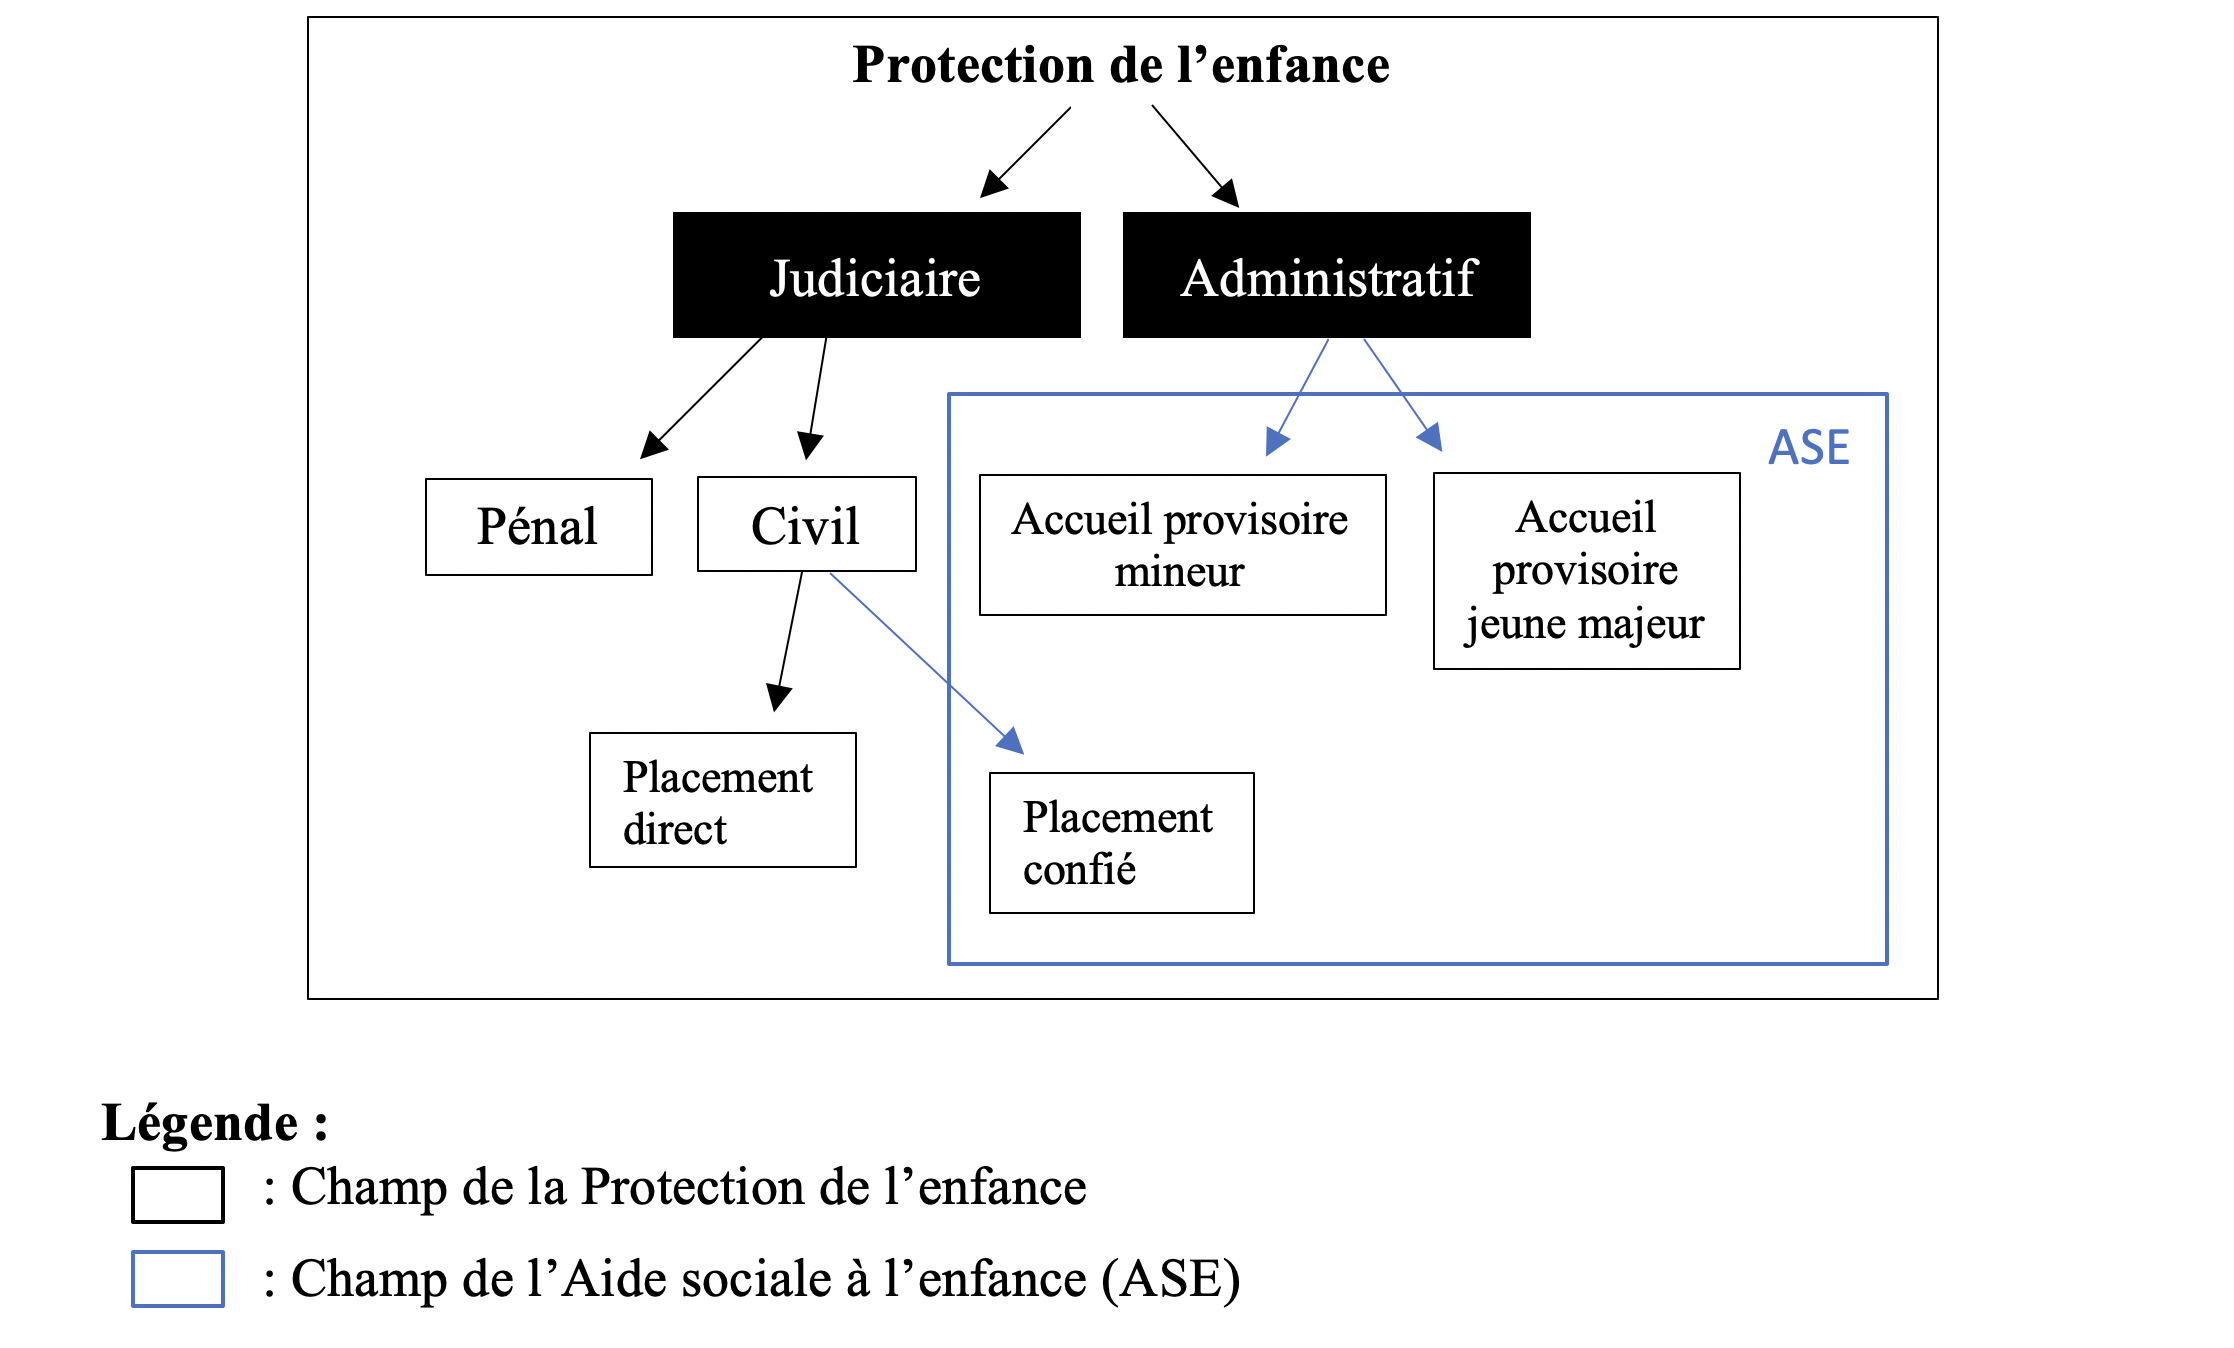
\includegraphics[width=0.9\linewidth]{Figure/SC1} 

}

\caption{L'organisation de la Protection de l'enfance en France}\label{fig:unnamed-chunk-8}
\end{figure}

\begin{quote}
\emph{La protection judiciaire}
\end{quote}

Nous le disions, la protection judiciaire s'occupe à la fois des enfants
délinquants et des enfants en danger mineurs ou jeunes majeurs. Dans les
deux cas, c'est le Tribunal pour enfants représenté par le Juge pour
enfants qui décide de la mesure éducative qui sera prise.

Pour les mineurs délinquants, la mesure prise peut être un placement
chez ses parents ou son tuteur, tout comme un placement sous liberté
surveillée (le mineur sera suivi par un éducateur dépendant directement
du tribunal) et/ou un placement dans une institution ou un établissement
public ou privé d'éducation ou de formation professionnelle habilité. La
mesure ne peut excéder l'âge de 18 ans.

Dans le cas des enfants en dangers mineurs ou jeunes majeurs, le juge
des enfants peut décider de mesures éducatives. En la matière, c'est
l'ordonnance de 1958 relative à la protection de l'enfance et de
l'adolescence en danger qui spécifie le champ et l'objectif de l'action
du juge des enfants. Elle indique ainsi que le champ d'action du juge
des enfants dépasse désormais le domaine du pénal et s'applique aussi à
celui du civil\footnote{Au vu du faible décrochage des pourcentages
  d'inertie, on aurait pu être tenté de prendre en considération en plus
  des deux premiers axes, les axes 3 et 4 dans le calcul de la CAH. Des
  tests ont été réalisés prenant d'abord en compte les 4 premiers axes
  de l'ACM puis les 3 premiers axes, les CAH alors calculées donnaient
  des classes peu pertinentes à l'interprétation en plus d'augmenter
  l'hétérogénéité intra classes.}. Ainsi, ce dernier doit vérifier qu'il
s'agit bien d'un cas d'enfant en danger ou en risque de danger. Une fois
cette première étape remplie, il peut orienter l'enfant en protection
administrative ou déterminer l'absence de danger et se retirer du
dossier. N'existant pas de définition claire d'enfant en situation de
danger, ce point est laissé à l'appréciation personnelle du juge des
enfants. Ce point ouvre à l'accueil d'enfants ayant vécu des situations
très diverses. Dans le cas d'un choix d'action de la part du juge, ce
dernier peut choisir de la faire appliquer avec ou sans l'accord des
parents ou des tuteurs légaux. Il doit néanmoins par la loi chercher le
plus possible l'adhésion de la famille. Ce point pose la question de la
prise en compte de ces derniers dans la décision de protection du juge
et sur la place qu'ils occuperont par la suite dans le parcours de
protection de leur enfant. Les enfants de la protection judiciaire
peuvent être pris en charge jusqu'à l'âge de 21 ans.

\begin{quote}
\emph{La protection administrative}
\end{quote}

Concernant, la branche administrative de la Protection de l'enfance,
cette dernière est gérée par l'Aide sociale à l'enfance (ASE),
anciennement appelée assistance publique. Elle a autant un rôle
préventif que protecteur\footnote{Marie-Paule Martin-Blachais et
  Jean-Marie Vauchez, {«~La structuration de la protection de l'enfance
  en France~»}, \emph{VST - Vie sociale et traitements}, 28 février
  2017, vol.~133, nᵒ~1, p. 13‑18.}. Pour appliquer une mesure, elle doit
impérativement obtenir le consentement des parents ou du/des tuteurs
légaux. Le rapport avec les parents ou les tuteurs légaux est ainsi
profondément différent dans la branche administrative.

Deux ensembles de moyens d'action sont menés par l'ASE~: les actions
collectives et les prestations individuelles. Les actions collectives
ont pour objectif la promotion sociale et l'insertion des enfants et des
familles. Les prestations individuelles sont soit des aides à domicile,
soit l'accueil de l'enfant dans des structures de l'ASE à la demande des
parents ou suite à une décision judiciaire\footnote{P. Verdier et F.
  Noé, \emph{L'aide sociale à l'enfance}, \emph{op.~cit.}}. C'est à ces
dernières que cette étude s'intéressera particulièrement.

L'ASE a connu une suite de changements législatifs importants également
depuis la fin de la Seconde Guerre mondiale, mais surtout
particulièrement lors de la décentralisation au début des années 1980.
En effet, depuis la loi du 22 juillet 1983, l'ASE est devenue un service
départemental. L'État laisse ainsi à la charge de chaque département
d'organiser ce service d'aide sociale obligatoire. L'objectif de l'ASE
est d'apporter un soutien matériel, éducatif et psychologique aux
mineurs et jeunes majeurs, à leur famille ou à leurs responsables légaux
qui seraient confrontés à des difficultés mettant ou risquant de mettre
en danger la sécurité, la santé, la moralité, l'éducation, le
développement physique affectif, intellectuel et social, des mineurs ou
jeunes majeurs. Le public concerné est aussi vaste que la mission de
l'ASE. Elle accueille ainsi les mineurs émancipés, les majeurs de moins
de 21 ans, les mineurs isolés, les femmes seules avec enfants de moins
de 3 ans.

\begin{quote}
\emph{Des critiques et des évolutions}
\end{quote}

La question de la protection de l'enfance est un sujet sensible dans
notre société, et ce, particulièrement depuis qu'elle fait l'objet d'une
politique publique claire. Ainsi, les critiques envers ce service d'aide
sociale ont été depuis longtemps virulentes, particulièrement envers le
fonctionnement de l'ASE. Elles dépeignent un service d'accueil violent,
qui agirait plus à l'encontre des familles qu'en leur faveur
\footnote{Pour réduire la dissimilarité intra-classe, le choix a été
  fait, après avoir choisi la partition, de consolider les résultats de
  la CAH par un algorithme des K-means. Cette dernière réaffecte les
  individus dans la classe dont ils se rapprochent le plus. On obtient
  ainsi des classes plus robustes.}. Pour y répondre, l'ASE a dû évoluer
autant dans sa manière de penser la protection de l'enfance que dans ses
actions concrètes, c'est-à-dire dans ses méthodes d'accueil. Ces
évolutions se sont traduites dans les textes de loi.

Tout d'abord avec la loi de 2002, qui revoit le cadre d'intervention en
réaffirmant les droits des usagers, qu'ils s'agissent de l'enfant
(mineur ou majeur) ou des familles et en assurant leur participation
dans la vie des établissements.

La réforme de la protection de l'enfance de mars 2007 confirme quant à
elle l'ensemble des dernières évolutions législatives et institue les
Conseils Généraux comme en charge du plan départemental. Elle pose aussi
trois axes prioritaires pour l'avenir de la Protection de l'enfance~:
renforcer les actions de prévention sur les territoires, organiser le
recueil des signalements des situations de danger sur les départements,
et diversifier les modes de prises en charge pour les adapter aux
besoins de chaque enfant en danger ou en risque de danger.

Cette loi sera enfin complétée par celle du 14 mars 2016 qui inscrit
notamment dans les missions de l'ASE de veiller à la stabilité du
parcours de l'enfant. Outre des réformes sur certains points légaux de
l'adoption, cette loi réécrit aussi l'article du code de l'action
sociale et des familles relatif au projet pour l'enfant (PPE) afin qu'il
serve l'intérêt supérieur de l'enfant. Enfin, un autre développement
majeur porté par la loi de 2016, est l'ajout aux missions des
observatoires départementaux de la protection de l'enfance d'une mission
pour la formation continue des professionnels de la PE\footnote{Pour des
  raisons d'effectifs, les tranches d'âge précédemment utilisées dans
  l'ensemble de ce mémoire n'ont pas pu être reprises dans ce modèle. On
  propose donc des tranches d'âge moins nombreuses qui regroupent les 0
  à 10 ans ensemble. Ce choix n'est pas sans conséquence. En effet, nous
  l'avons vu les plus jeunes enfants sont particulièrement présents dans
  la classe 1 de notre CAH et pas dans les classes 2 et 3. Or, ces
  derniers se retrouvent ici englobé dans une catégorie bien plus large.}.

\hypertarget{un-duxe9veloppement-en-lien-avec-luxe9volution-de-la-notion-de-famille-et-de-la-perception-de-lenfance}{%
\subsection{Un développement en lien avec l'évolution de la notion de
famille et de la perception de
l'enfance}\label{un-duxe9veloppement-en-lien-avec-luxe9volution-de-la-notion-de-famille-et-de-la-perception-de-lenfance}}

\begin{quote}
\emph{Les évolutions de la famille contemporaine et l'intervention
croissante de l'état}
\end{quote}

Ces lois ont été inspirées par les évolutions de perception de la
famille et de l'enfance par la société. Ainsi, pour comprendre
l'institution qu'est la Protection de l'enfance et son champ
professionnel, il faut saisir l'arrière-fond des connaissances, des
savoirs, des normes sociales, voire des prescriptions, en matière de
famille et d'enfance, puisque cet arrière-fond sous-tend leur action.
Nous nous concentrerons d'abord sur la famille avant de porter notre
regard sur l'enfance.

Bien qu'il serait pertinent d'effectuer un retour historique, déjà
mainte fois réalisé, sur la famille au travers des sociétés médiévales
et modernes\footnote{Philippe Ariès, \emph{L'enfant et la vie familiale
  sous l'Ancien régime}, Nouv. éd., {Paris}, {Éd. du Seuil}, 2014,
  316~p.}, tant il éclaire la forme actuelle de la famille
contemporaine, nous nous attarderons sur les évolutions récentes de
l'institution familiale depuis le début du XX\textsuperscript{e} siècle.
En effet, durant ce siècle, la famille a connu des changements majeurs
qui peuvent être résumés dans des facteurs démographiques~: la baisse du
taux de mortalité infantile et du taux de natalité, la diffusion des
méthodes modernes de contraception, la légalisation de l'avortement, la
réduction de la taille de la famille. Parallèlement à ces éléments,
l'émergence de l'État providence a poussé à une plus forte implication
de l'État dans les sujets sociaux\footnote{Gøsta Esping-Andersen,
  \emph{Les trois mondes de l'État-providence}, {Paris}, {Presses
  Universitaires de France}, 2007.}. Ainsi, en France, dans l'exemple
des politiques concernant la jeunesse, ces dernières suivent une logique
«~sociale-démocrate~» et tendent à atténuer la dépendance du jeune à sa
famille avec des aides directes de l'État\footnote{Cécile Van de Velde,
  \emph{Soutenir l'autonomie des jeunes majeurs : puissance et
  impuissance du politique}, s.l., {Champ social}, 2012.}.\footnote{Lucy
  Marquet, Zoé Perron et Isabelle Frechon, {«~Les Enfants Protégés En
  {France}. {Différences} Selon Les Politiques Départementales de Prise
  En Charge~»}, {Aix-en-Provence, France}, 2013.} Un cadre législatif et
de nombreuses réformes ont été mises en place et ont fait évoluer la
forme et l'action de la Protection de l'Enfance, et ce, particulièrement
depuis la fin de la Seconde Guerre mondiale. Ces évolutions aboutissent
à la mise en place de la contemporaine, pour reprendre les réflexions de
François de Singly. Ce dernier démontre le phénomène d'intervention
croissante de l'État dans la famille qui se fait en parallèle avec une
privatisation de cette dernière\footnote{François de Singly,
  \emph{Sociologie de la famille contemporaine}, 6e éd., {Malakoff},
  {Armand Colin}, 2017.}. C'est dans ce double mouvement que la
Protection de l'enfance s'inscrit en ce faisant un outil de
l'intervention étatique au sein de l'institution familiale. Émile
Durkheim percevait déjà la famille comme à la fois privée et publique~:
privée, car il constatait son autonomisation vis-à-vis des voisins,
publique, parce que sa dépendance à l'État ne cessait de
croître\footnote{Émile Durkheim, {«~La Famille Conjugale~»}, \emph{Revue
  philosophique}, 1921, 1892, nᵒ~90, p. 9‑14.}. Pour F. de Singly, plus
qu'un rôle d'aide, l'État encadre, voire étend son contrôle sur les
familles, il se fait ainsi le régulateur des relations familiales. Ce
contrôle croissant de la parentalité se fait en parallèle de nombreuses
réformes sociales qui garantissent l'autonomisation de l'homme et de la
femme en tant que conjoints\footnote{F. de Singly, \emph{Sociologie de
  la famille contemporaine}, \emph{op.~cit.}}.

On peut ainsi s'interroger sur les effets que produit cette intervention
croissante de l'État dans une perspective critique. Si ces évolutions
peuvent s'apparenter à un développement positif des libertés
individuelles et du respect des droits de l'Homme avec une protection
légale renforcée des enfants, il existe un versant négatif à cette
intervention. En effet, comme Franz Schultheis l'a souligné, elle
augmenterait les risques socioéconomiques pour les familles en
facilitant la séparation conjugale. Ce risque selon lui dépend du sexe,
de la situation familiale ou encore du statut socioéconomique. Il
s'appuie sur l'exemple des mères célibataires qui font face à de lourdes
difficultés économiques. Ce risque rejaillit sur l'enfant et nécessite
pour l'équilibrer une intervention de l'État\footnote{Franz Schultheis,
  {«~Affaires de famille et raison d'État: Les enjeux privés et publics
  dans l'invention d'un nouveau type de risque : le « risque familial
  »~»}, \emph{Sociétés \& Représentations}, 1997, vol.~5, nᵒ~2, p. 225.}.
Ici, de nouveau, la Protection de l'enfance tendrait à pallier ce
déséquilibre.

Outre ces points, la société chercherait dès lors à responsabiliser
d'autant plus les parents vis-à-vis de leur·s enfant·s. En effet, en
contrepartie d'un gain de liberté individuelle par une plus grande
facilité de se séparer de son.sa conjoint·e, les deux parents doivent
assurer une continuité parentale auprès de leur·s enfant·s. C'est ce que
souligne particulièrement Irène Thery, pour qui dès lors le bien le plus
précieux de la famille est l'enfant qui devient le socle
familial\footnote{Irène Théry, \emph{Le Démariage}, s.l., {Odile Jacob},
  1993.}. Ainsi, les attentes envers l'éducation des enfants augmentent,
justifiant d'autant plus une intervention de la Protection de l'enfance
afin d'assurer une égalité de traitement dans les cas où ces attentes ne
seraient pas remplies.

Du fait de ces évolutions sociétales, le droit a dès lors poussé les
États-providence à agir en matière de protection de l'enfant. La
Convention internationale de l'enfant de 1989 (CIDE)\footnote{Les effets
  de la variable portant sur le sexe des enfants placés ne sera pas
  présenté dans les tableaux suivants bien que présente en tant que
  variable de contrôle lors du calcul du modèle. Ce choix est motivé par
  la volonté malgré un nombre important de variable explicative incluses
  dans le modèle de présenter un tableau clair, mais aussi par le fait
  que la variable de sexe n'a aucun effet significatif dans ce modèle.},
pour ne citer qu'elle, parachève un ensemble de textes internationaux
qui visent à garantir les droits en tant que citoyen de l'enfant. Ceci
s'explique par une notion mise en avant par la CIDE de 1989 ratifié par
la France en 1990 qui est celle de l'«~intérêt de l'enfant~». Dans le
droit français, cette notion apparaît déjà avec la loi de 1904 portant
sur l'organisation de l'Assistance publique, future Aide sociale à
l'enfance. Ce principe est devenu rapidement un leitmotiv des politiques
publiques. Il apparaît dans les textes de loi et fonde plusieurs de ses
principes d'action et définit les objectifs de prise en charge de
l'enfant.

\begin{quote}
\emph{Les représentations de l'enfance et leurs effets sur les pratiques
professionnelles}
\end{quote}

L'ensemble de ces réflexions nous amène à nous concentrer plus
particulièrement sur l'enfant et les représentations de l'enfance. Ces
dernières changent et évoluent d'une culture à une autre. La dimension
historique dans le cas français le met clairement en
évidence\footnote{P. Ariès, \emph{L'enfant et la vie familiale sous
  l'Ancien régime}, \emph{op.~cit.}}, notamment dans l'évolution qu'a
connu l'âge du passage à la majorité et donc de la fin du statut
d'enfant. L'enfance est ainsi une catégorie sociale, qui par rapport aux
autres catégories sociales a la particularité d'être vécue par tout le
monde une fois dans leur vie. Pour aller plus loin dans cette définition
de l'enfance, on peut reprendre les réflexions de Virginie Vinel et
Francesca Zaltron, pour qui l'enfant est un individu qui appartient à
une strate sociale relative à la société et à une époque
donnée\footnote{Virginie Vinel et Francesca Zaltron, {«~Enfants acteurs,
  enfants agis~»}, \emph{Revue des sciences sociales}, 15 juin 2020,
  nᵒ~63, 63, p. 12‑25.}.

Ce sont donc les adultes qui fondent les représentations de l'enfance et
créé les contours de cette catégorie. Il est intéressant de noter ici,
que depuis la fin du XIX\textsuperscript{e} siècle et durant tout le
XX\textsuperscript{e} siècle jusqu'à nos jours, l'enfant est défini aux
yeux de la société par un ensemble de savoirs psychologiques et médicaux
qui dressent des stades de développement aboutissant à l'adulte, pour
reprendre la réflexion de André Turmel\footnote{Turmel André, \emph{Une
  Sociologie Historique de L'enfance.}, {Quebec}, {Les Presses de
  l'Université Laval}, 2013.}. Ces derniers régularisent et
standardisent les phases physiques et psychologiques de l'enfant. Ils
permettent aussi de définir les besoins vitaux tant en termes physiques
qu'émotionnels de l'enfant en fonction de son âge, des besoins auxquels
la famille se doit de répondre, et à défaut d'elle, auquel l'État doit
suppléer. C'est sur ces connaissances transmises dans le cadre de leur
formation que les professionnels encadrants les mineurs s'appuient et
qui définit leur mode d'action.

Ces évolutions de la perception de l'enfance ont été étudiées par les
sociologues notamment avec les \emph{childhood studies} dans lesquelles
deux visions s'affrontent~: soit observer les enfants comme des adultes
en formation, soit étudier les enfants en tant qu'être présents, en lien
avec la notion d'\emph{agency}\footnote{Wilfried Lignier, Cédric Lomba
  et Nicolas Renahy, {«~The Social Differentiation of Children~»},
  \emph{Politix}, 23 octobre 2012, vol.~99, nᵒ~3, p. 9‑21.}. Il est
intéressant de voir dès lors des études cherchant à souligner l'effet
des différents regards portés sur les enfants dans la recherche, les
institutions, les sociétés et comment ces différents regards se
diffusent et questionnent les acteurs des champs qui encadrent les
mineurs\footnote{V. Vinel et F. Zaltron, {«~Enfants acteurs, enfants
  agis~»}, art cit.}. En effet, le travail des professionnels du secteur
de la protection de l'enfance témoigne de l'évolution de ces visions de
la société. Pour reprendre les mots de Jérôme Delfortie~:
«~\emph{L'édifice Protection de l'Enfance a évolué au gré des
différentes lectures de l'enfance par le prisme social.}~»\footnote{Jérôme
  Delfortrie, {«~De la Protection de l'Enfance à la protection de
  l'enfant~»}, \emph{Le Sociographe}, 30 novembre 2017, vol.~10, nᵒ~5,
  p. 31‑60.}.

Ainsi, bien que l'on parle d'enfance en générale, les professionnels
font dorénavant des distinctions entre bébé, enfance, adolescence et
jeune adulte. Des distinctions que l'on retrouve par ailleurs dans les
sciences sociales et qui permettent de mieux appréhender des réalités
sociales très différentes entre ces différentes périodes de vie.

Les relations entre adultes et enfants ont du fait de ces savoirs sur
l'enfance évolué, que cela soit dans le champ familial ou professionnel.
L'État a augmenté aussi sonintervention, ce qui a conduit à judiciariser
les rapports avec enfant, pour reprendre les termes de Alain Renaut. Un
point qui a eu pour effet sa libération de l'autorité
traditionnelle\footnote{Alain Renaut, \emph{La Libération Des Enfants:
  Contribution Philosophique à Une Histoire de l'enfance}, {Paris},
  {Calmann-Lévy : Bayard}, 2002, 396~p.}. C'est cette libération qui a
court depuis le XIX\textsuperscript{e} siècle et est même datée par
certains à la loi du 24 juillet 1889 où l'État instaure la déchéance des
droits de la puissance paternelle, qui rend possible l'intervention de
la Protection de l'Enfance en la matière. En effet, l'État devient dès
lors le protecteur des enfants en situation de danger ou risque de
danger\footnote{M.-P. Martin-Blachais et J.-M. Vauchez, {«~La
  structuration de la protection de l'enfance en France~»}, art cit.}.

\hypertarget{lorganisation-concruxe8te-du-placement}{%
\subsection{L'organisation concrète du
placement}\label{lorganisation-concruxe8te-du-placement}}

\begin{quote}
\emph{Parcours type en Protection de l'enfance}
\end{quote}

Jusqu'à présent, nous avons vu l'organisation globale de la Protection
de l'enfance, les types d'enfants dont elle s'occupait et les évolutions
de la société dans la perception de l'enfance et de la famille qui
explique son mode d'action. Dans tout cela, le parcours en soi de
placement n'a pas été abordé. Ce dernier suit un déroulement typique qui
va du signalement et de l'évaluation de la situation à sa réévaluation
avant la sortie de placement ou la mise en place d'une nouvelle mesure.

\textbf{Figure -- Schéma du parcours type de placement en Protection de
l'enfance}

\begin{figure}

{\centering 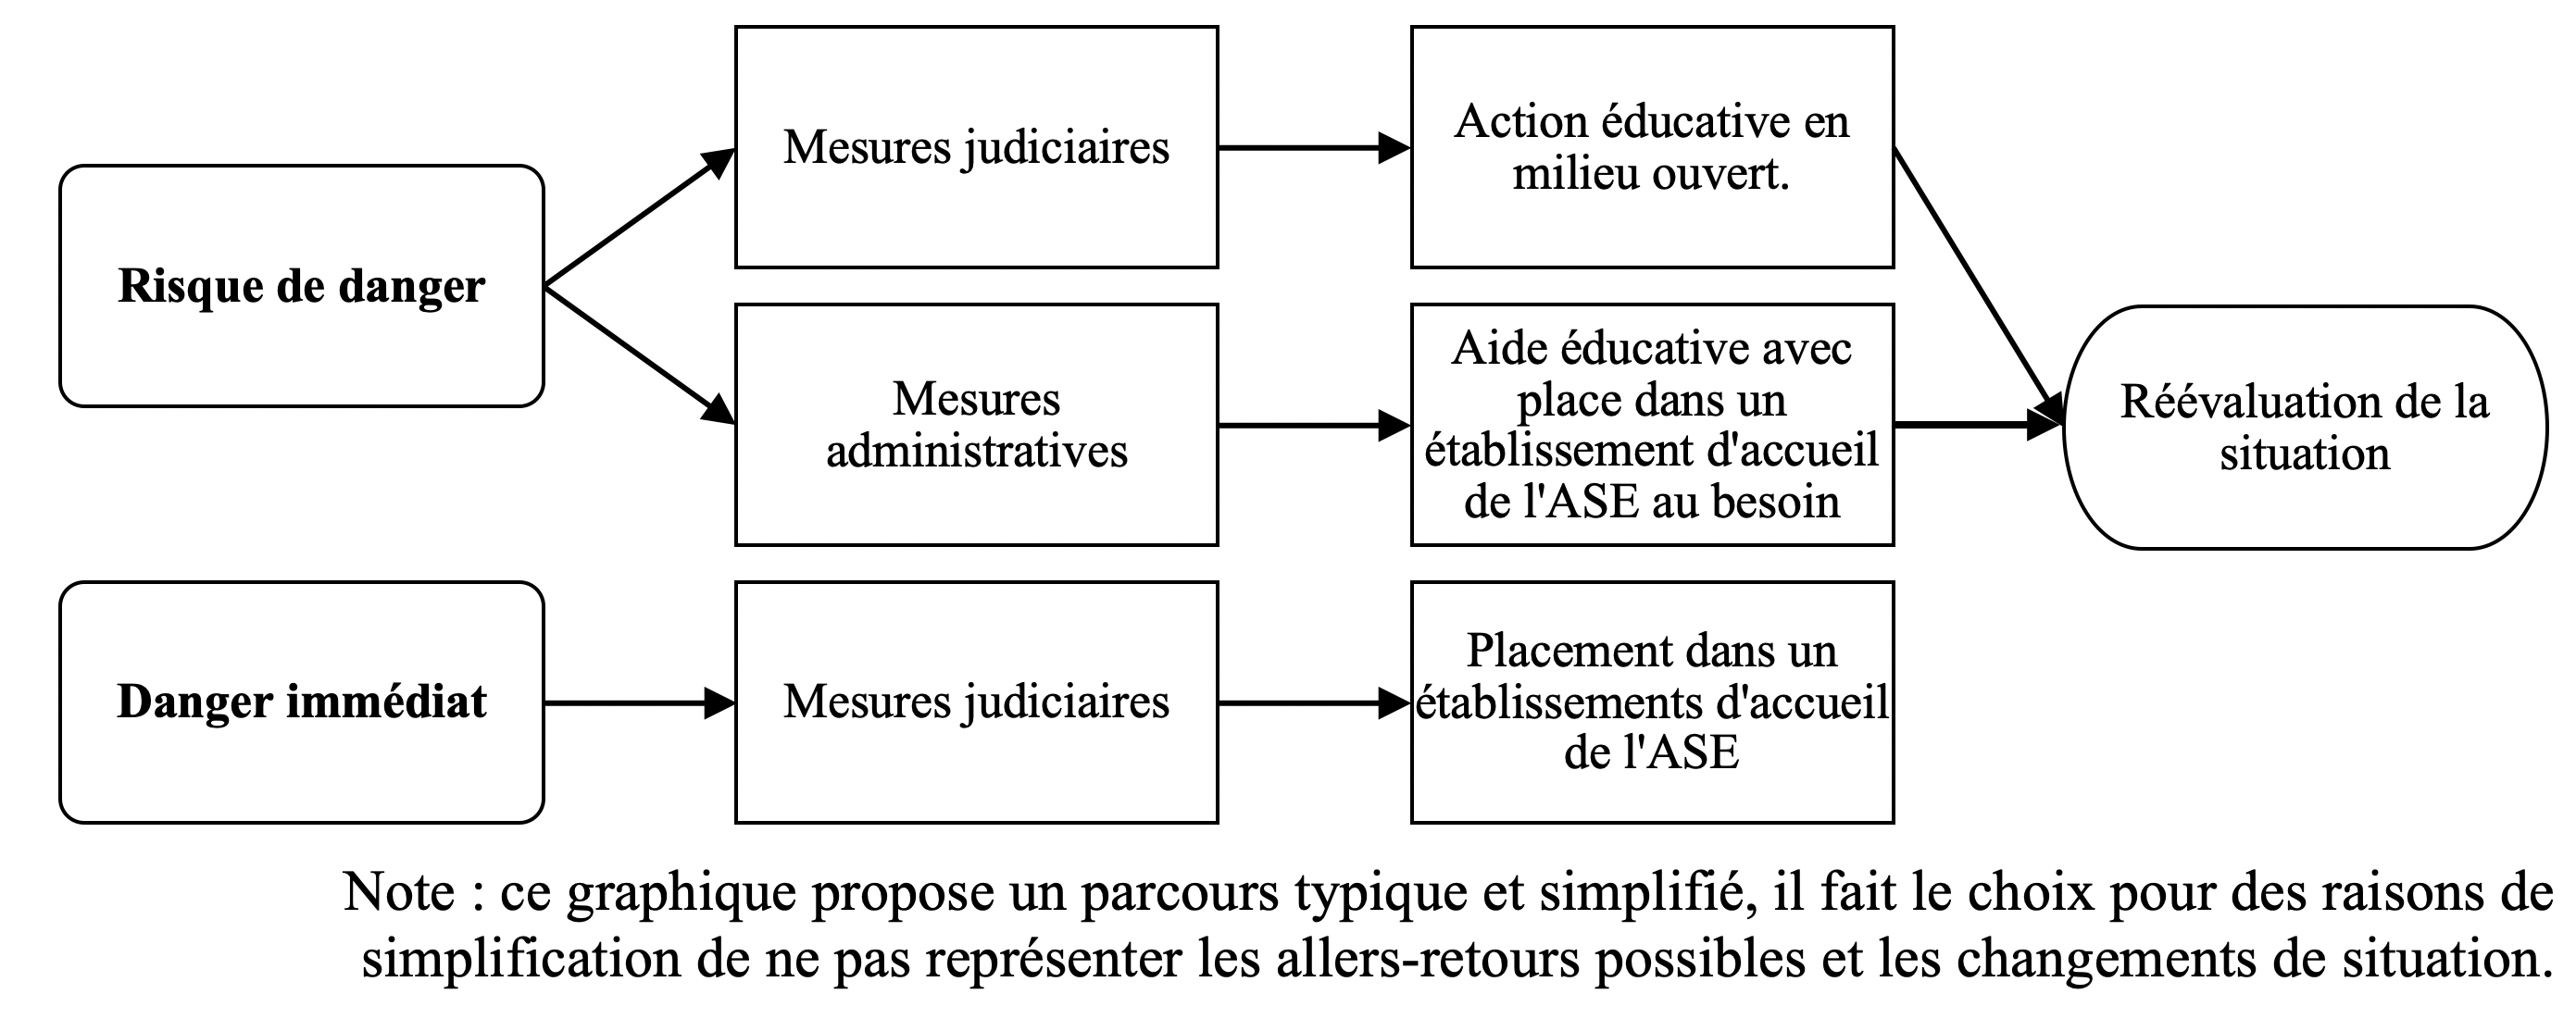
\includegraphics[width=0.9\linewidth]{Figure/SC2} 

}

\caption{Schéma du parcous type de placement en Protection de l'enfance}\label{fig:unnamed-chunk-9}
\end{figure}

Ainsi, après un signalement, la Cellule de recueil des informations
préoccupantes (Crip) enquête sur la situation de l'enfant. Cette
première étape consiste à une visite d'une assistante sociale au
domicile de l'enfant, elle tente alors de déterminer s'il y a risque de
danger ou danger immédiat. Mais aussi, elle cherche à savoir si les
parents sont enclins à accepter une aide. Suite à cette visite,
l'assistante sociale fait remonter en cas de risque de danger ou danger
immédiat l'information, afin qu'une aide soit mise en place.

S'il y a selon elle danger immédiat, l'affaire est envoyée au juge des
enfants qui jauge la situation et tente de mettre en place une mesure de
commun accord avec les parents ou tuteurs légaux. Dans le cas du danger
immédiat, c'est néanmoins le juge des enfants qui a le dernier mot en la
matière, il n'a donc pas besoin de recueillir l'aval des parents ou
tuteurs légaux. Une mesure judiciaire va être prise qui débouche sur un
placement en famille d'accueil, Maison d'enfant à caractère sociale,
pouponnières ou villages d'enfants.

S'il y a risque de danger, une assistance éducative va être proposée par
le département et être appliquée généralement sous la forme d'une aide
éducative à domicile si les parents sont d'accord. Si les parents
refusent ou que l'aide éducative à domicile échoue, l'affaire peut être
transférée au juge des enfants qui peut dès lors prendre une mesure sans
l'aval des parents. Généralement, une mesure d'action éducative en
milieu ouvert, couramment appelée AEMO, est mise en place.

La situation de l'enfant est à la fin réévaluée. Si le risque de danger
persiste ou que l'AEMO est un échec, l'affaire est renvoyée devant le
juge des enfants qui reconduit la mesure ou décide d'un placement.

Le processus de placement suit ainsi un parcours type qu'Émilie Potin
s'est attachée à décrire d'un point de vue sociologique prenant en
compte l'expérience de l'enfant. Elle décrit ainsi le parcours de
placement~comme traversé par trois phases principales : «~la désignation
du danger (processus d'étiquetage)~», puis le «~déplacement d'un lieu à
l'autre et d'un milieu social à l'autre (processus d'apprentissage,
d'adaptation et de socialisation)~» et enfin~:~«~l'intégration dans le
quotidien du placement (phase de routinisation)~»\footnote{Émilie Potin,
  \emph{Enfants En Danger, Enfants Protégés, Enfants Sécurisés ? :
  Parcours de (Dé)Placement(s) Des Enfants Confiés à l'{Aide} Sociale à
  l'enfance}, These de doctorat, {Brest}, s.l., 2009.}. Le processus
d'étiquetage appelle par la suite à un déplacement dans une structure. À
l'aide de l'étiquette attribuée à la situation de l'enfant, l'ASE
appelle ensuite les structures qu'elle juge adaptées à accueillir
l'enfant afin d'appliquer la décision de protection. Les structures
elles-mêmes acceptent ou non d'accueillir l'enfant en fonction de leur
jugement en leur capacité d'accueillir l'enfant, leurs places
disponibles et le public déjà accueilli. Elles orientent alors l'enfant
dans un type d'hébergement.

\begin{quote}
\emph{Les catégories juridiques des enfants accueillis}
\end{quote}

De ce système de protection résulte sept catégories juridiques d'enfants
protégés divisé en deux catégories~en fonction des deux branches de la
Protection de l'enfance : les mesures judiciaires et les mesures
administratives (voir Tableau 1). Pour la recherche scientifique, ces
catégories juridiques font l'objet de réflexion, puisqu'on les retrouve
dans~les données produites sur le sujet. Ainsi, la question de leur
utilisation et de leur signification sociologique se pose comme le
souligne I. Frechon\footnote{Isabelle Frechon, {«~L'impossible
  observation de l'enfance protégée en France ?~»}, 2002, p. 15.}. Le
problème majeur de ces catégories est qu'elles concentrent des enfants
aux situations très diverses dans les mêmes groupes. Ce point rend
difficile de les utiliser pour définir les enfants pris en charge,
néanmoins, il rend utile de tels variables afin de porter son regard sur
les pratiques des professionnels et surtout les différences entre
pratiques du secteur judiciaire et du secteur administratif.

\begin{longtable}[]{@{}
  >{\raggedright\arraybackslash}p{(\columnwidth - 4\tabcolsep) * \real{0.1944}}
  >{\raggedright\arraybackslash}p{(\columnwidth - 4\tabcolsep) * \real{0.1944}}
  >{\raggedright\arraybackslash}p{(\columnwidth - 4\tabcolsep) * \real{0.6111}}@{}}
\toprule
\begin{minipage}[b]{\linewidth}\raggedright
\textbf{Tableau 1 - Les catégories juridiques des enfants accueillis}
\end{minipage} & \begin{minipage}[b]{\linewidth}\raggedright
\end{minipage} & \begin{minipage}[b]{\linewidth}\raggedright
\end{minipage} \\
\midrule
\endhead
\textbf{Type de mesure} & \textbf{Catégorie juridique} &
\textbf{Définition} \\
MESURES JUDICIAIRES & \emph{Les mineurs délinquants} pris en charge
directement par le juge (Ord. de 1945 du code pénal) & Prise en charge
décidée, suivie et financée par la justice, pour une mesure qui peut
être soit un hébergement physique en secteur public ou associatif
habilité, ou une liberté surveillée \\
& \emph{Les enfants confiés à l'ASE par le juge} & Prise en charge sera
décidée par le juge des enfants mais une fois confié, c'est l'ASE qui
orientera l'enfant, financera et suivra la prise en charge. Cette
catégorie réunis les enfants en danger (Art. 375 et suiv. du code civil)
et les mineurs délinquants (Ord. de 1945 du code pénal). Placement en
établissement ou famille d'accueil. \\
& \emph{Les enfants placés directement par le juge des enfants} &
Concerne uniquement les enfants en danger (Art. 375 et suiv. du Code
civil) dont la décision et le suivi éducatif de prise charge sont
assurés par le juge des enfants. L'enfant est alors orienté soit en
secteur public PJJ ou en secteur associatif habilité. Dans ce dernier
cas, c'est l'ASE qui financera, contrôlera et suivra l'enfant. \\
& \emph{Les jeunes majeurs PJJ} (Décret du 18 février 1975) & Âgés entre
18 et 21 ans, ils ont fait la demande de protection auprès du juge des
enfants qui a la charge dans son ensemble de la prise en charge
(décision, suivi et financement). \\
MESURES ADMINISTRATIVES & \emph{Les pupilles de l'État} & Enfants
orphelins, ou dont aucun de leurs deux parents n'exerce d'autorité
parentale, ni même un tiers digne de confiance. Le préfet est alors
tuteur des pupilles de l'Etat et le président du conseil généralen est
le gardien. Il délègue ainsi sa fonction à l'ASE. Les décisions de prise
en charge, le suivi et le financement reviennent donc intégralement à
l'ASE. \\
& \emph{Les accueils provisoires de mineurs} & Il s'agit des enfants «
en risque de danger », la décision (avec l'accord des parents) d'une
prise en charge, le suivi et le financement reviennent intégralement à
l'ASE. \\
& \emph{Les accueils provisoires de jeunes majeurs} (Décret du 2
décembre 1975) & De même que pour les jeunes majeurs PJJ, il s'agit de
jeunes de 18 à 21 ans qui font la demande à l'ASE d'être protégé. La
décision d'une prise en charge, le suivi et le financement sera assuré
par l'ASE. \\
\bottomrule
\end{longtable}

Il est à noter que quand bien même un enfant entre à la Protection de
l'enfance dans une catégorie juridique, cette dernière n'est pas
immuable. Il peut ainsi, au moment de la réévaluation de sa situation,
se retrouver dans une autre catégorie pour pouvoir poursuivre sa prise
en charge à la Protection de l'enfance dans les meilleures conditions.

~~~~~~\emph{Définitions des différents types d'établissements et
d'hébergements}

Nous venons brièvement de l'évoquer dans le parcours type de placement,
mais il existe différents lieux d'accueil qui sont destinés à accueillir
les enfants en fonction de leurs besoins individuels, c'est-à-dire en
fonction de leur âge, de leur motif de placement et d'éventuelles
particularités dans leur situation~: mineurs non accompagnés, situation
de handicap.

Si on structure ce tour d'horizon des types d'établissements de
placement de l'ASE par âge, il convient de débuter avec les
pouponnières. Ces dernières sont spécialisées dans l'accueil des enfants
de 0 à 3 ans, ce sont des structures de taille moyenne avec comme
capacité autorisée en 2017 une moyenne de 23 places, n'excédant pas les
30 places dans 75\% des cas en 2017.

Ensuite, les villages d'enfants sont peu nombreux sur le territoire, 37
structures en tout. Ils sont spécialisés dans l'accueil des enfants sur
le long terme. Ce sont de grands lieux d'accueil avec une capacité
moyenne de 57 enfants par structure répartis en unité de vie, ce qui
permet de proposer néanmoins un accueil personnalisé et une stabilité
dans le placement.

Les lieux de vie et d'accueil proposent quant à eux un accueil
individualisé des enfants dans de petites structures ayant en moyenne 6
places et qui ne peuvent accueillir plus de 7 enfants. Ils accueillent
les enfants avec des problèmes psychologiques ou ceux que l'on considère
comme des «~incasables~», c'est-à-dire qu'ils multiplient les types de
placement, sans qu'aucun ne semble parvenir à s'adapter à leurs besoins.

Les Foyers de l'enfance sont des hébergements d'urgence et courts qui
accueillent surtout avant réorientation les enfants vers un type
d'accueil plus pérennes. Ce sont des structures de taille variable avec
une capacité moyenne de 58 enfants. 25\% de ses structures ne dépassent
pas les 12 enfants en capacité d'accueil autorisée et 25\% dépassent à
l'inverse les 63 enfants en capacité d'accueil autorisée.

Enfin, les Maisons d'enfant à caractère social (MECS), proposent un
accueil temporaire d'enfant lié à un problème familial ou
comportemental. Ils accueillent aussi les mineurs non accompagnés. Ils
ont une capacité moyenne d'accueil de 41 enfants avec aussi une grande
variabilité en 2017 dans la taille des structures~: un premier quart de
structures ne dépassant pas 18 places en capacité autorisée, la moitié
les 35 places et enfin les trois-quarts les 56 places.

Le premier type d'hébergement le plus courant et proposant le plus de
places est l'internat collectif. C'est un hébergement au sein de la
structure qui peut proposer plusieurs unités de vie, c'est le cas
notamment dans les villages d'enfant. On le retrouve dans tous les types
d'établissements.

Les assistants familiaux sont le deuxième type d'hébergement proposé.
Ces derniers sont des professionnels de la protection de l'enfance
formés par l'État à l'accueil de mineurs ou jeunes majeurs protégés. Ils
accueillent directement chez eux les jeunes majeurs ou mineurs. Ils
restent rattachés dans certains cas à des établissements qui gèrent le
placement de l'enfant et on les retrouve aussi dans tous les types
d'établissements.

Le placement à domicile est une mesure d'assistance éducative décidée
par un juge pour enfant. Concrètement, le jeune majeur ou le mineur
continue de vivre dans sa famille, mais bénéficie d'une solution de
repli dans un établissement de l'ASE. C'est un type d'hébergement que
l'on retrouve dans tous les types d'établissements, sauf en lieux de vie
et d'accueil.

Enfin, le logement autonome ou hébergement éclaté recoupe plusieurs
réalités. Il s'agit de place d'hébergement physiquement en dehors de la
structure d'accueil, soit dans un ensemble de logements, soit en
chambres dispersées dans le logement ordinaire ou l'habitat social,
voire en hôtel. C'est un type d'hébergement qui n'est logiquement pas
proposé par les pouponnières à caractère social et est peu présent dans
les villages pour enfants.

\hypertarget{les-maisons-denfant-uxe0-caractuxe8re-social-mecs-un-type-de-placement-aux-enjeux-particuliers}{%
\section{Les Maisons d'enfant à caractère social (MECS), un type de
placement aux enjeux
particuliers}\label{les-maisons-denfant-uxe0-caractuxe8re-social-mecs-un-type-de-placement-aux-enjeux-particuliers}}

\hypertarget{que-sont-les-mecs}{%
\subsection{Que sont les MECS ?}\label{que-sont-les-mecs}}

~~~~~~\emph{La définition progressive de l'action des MECS}

L'acronyme MECS désignant les Maisons d'enfant à caractère social existe
depuis 1957, mais l'institution d'aide à l'enfance qu'il désigne n'a
cessé d'évoluer depuis. Les MECS se sont construites sur un héritage
asilaire et à partir des hôpitaux, orphelinats et encore des maisons de
correction\footnote{Martial Chenut, \emph{Les MECS au cœur des
  évolutions de la protection de l'enfance}, {Toulouse}, 2018.}.

De manière générale, les missions des MECS sont les suivantes~:

\begin{itemize}
\item
  Mission de protection physique et psychologique.
\item
  Mission d'éducation, d'accès à une autonomie progressive.
\item
  Mission d'accompagnement social et d'insertion professionnelle.
\item
  Mission de régulation, restauration des relations intrafamiliales.
\end{itemize}

L'ensemble de ces missions indique une volonté que l'accueil en MECS
soit le plus possible temporaire en cherchant à préserver ou à restaurer
les liens familiaux. À terme, ceux-ci devraient permettent de réunir les
conditions affectives, psychologiques, sociales et matérielles
nécessaires au retour du mineur dans sa famille. Les MECS poursuivent
aussi une mission de prévention ou de lutte contre diverses formes de
marginalité, telle que la délinquance ou l'exclusion sociale. Il s'agit
ainsi de rétablir une place « ordinaire » dans la société pour les
mineurs et leurs familles en difficultés.

Pour saisir d'où proviennent les missions et compétences confiées aux
MECS aujourd'hui, il faut revenir quelque peu sur les différentes
évolutions que cette institution a connu depuis que son acronyme existe.
Les MECS des années 1960 sont d'abord des instituts d'accueils d'enfants
dit «~cas social~», c'est-à-dire des enfants dont les parents ne peuvent
s'en occuper pour de multiples raisons~: parents séparés, malades,
famille trop nombreuse, problèmes économiques\ldots{} Les enfants qui se
retrouvent dans ces instituts bénéficient alors d'un accueil de type
internat collectif pour une durée variable allant de quelques mois à des
années.

Dans un mémoire dédié au MECS, Martine Tourret souligne justement que
dès 1960, les rares et vagues textes qui réglementent les MECS intègrent
à la définition du type d'enfant accueilli la question du lien familial
qui se doit d'être préservé le plus possible\footnote{Martine Tourret,
  {«~Les {Maisons} d'enfant à Caractère Social Face à l'innovation~»}.}.
En témoigne jusqu'à présent le pourcentage qui reste faible d'enfants
orphelins accueillis, ces derniers étant plutôt orientés vers des
placements en assistants familiaux ou familles d'accueil.

Dans les années 1970, la définition des enfants accueillis en MECS, fait
l'objet d'âpres débats. Elle est perçue comme trop floue, englobant un
nombre incalculable de situations diverses et incomparables rendant
difficile leur prise en charge. Le rapport Dupont-Fauville est le fer de
lance de ces critiques et dresse un constat clair sur le
sujet\footnote{À noter qu'une version réduite de ce modèle est proposée
  dans les Annexes (voir Annexes - ).}. Le terme «~cas social~» a dès
lors été revisité, participant à faire évoluer le nom des MECS de
«~maison d'enfant à cas social~» à «~maison d'enfant à caractère
social~». Une évolution qui n'enlève pas en soi le côté flou d'une telle
désignation.

Les MECS sont souvent désignées par les acteurs de la profession comme
le~«~parent pauvre~» des structures de la Protection de
l'enfance\footnote{Francis Batifoulier et al., {«~Introduction~»},
  \emph{Empan}, 20 mars 2012, vol.~85, nᵒ~1, p. 10‑11.}. En effet, ces
institutions ont été directement touchées par les évolutions des
politiques publiques en matière de protection de l'enfance, telle que la
départementalisation de la Protection de l'enfance ou encore l'ouverture
des maisons d'enfants 365 jours par an. De plus, elles sont
régulièrement au cœur des tensions budgétaires. Outre ces défis
techniques et pratiques, s'ajoutent des difficultés liées au public
accueilli. Ce dernier ne cesse d'évoluer, souvent plus vite que les
structures elles-mêmes. Ainsi, l'incertitude de la durée de la prise en
charge, l'impossibilité récurrente de proposer en interne des soins
nécessaires face à l'évolution importante des troubles des enfants et
adolescents reçus, la hausse continue de la part de mineurs isolés
étrangers ou mineurs non-accompagnés, majoritairement pris en charge en
MECS\footnote{\emph{Ibid.}}.

~~~~~~\emph{Le cas des mineurs non accompagnés (MNA) ou mineurs isolés
étranger (MIE)}

Parmi toutes ces situations engendrant une prise en charge par la
Protection de l'Enfance, le cas des Mineurs isolés étrangers ou mineurs
non-accompagnés reste à part. Il s'agit d'enfants supposés mineurs,
arrivés sur le territoire français sans leurs parents ou tuteurs légaux.
Ils sont pris en charge en France par la Protection de l'enfance et/ou
ils entrent dans le système des demandeurs d'asile. La prise en charge
des MNA par la Protection de l'enfance a bouleversé les pratiques des
professionnels. En effet, l'action publique semble se perdre en la
matière entre politique d'immigration et politique de Protection de
l'enfance qui dans le cas présent ont des logiques contradictoires.

En effet, depuis 1990, selon Clémence Helfter, la France se retrouve
confrontée à l'arrivée sur son territoire de ce type de
migration\footnote{Clémence Helfter, {«~La prise en charge des mineurs
  isolés étrangers par l'Aide sociale à l'enfance~»}, \emph{Informations
  sociales}, 11 octobre 2010, n° 160, nᵒ~4, p. 124‑132.}. Leur nombre ne
faisant qu'augmenter, le débat public s'est emparé du sujet
particulièrement à partir de 2010. À partir de cette même période, de
nombreuses circulaires et textes de loi concernant la Protection de
l'enfance se modifient afin d'adapter les types de prise en charge à
cette population en constante augmentation. Ce sont les services de
l'Aide sociale à l'enfance qui ont été chargés de leur protection. Mais
pour que les MNA accèdent à cette prise en charge, encore faut-il qu'ils
soient reconnus comme tel, ce qui en l'absence de document justifiant de
leur âge représente souvent un obstacle insurmontable.

L'accueil des MNA a particulièrement reposé sur les MECS, qui proposent
un accueil temporaire en collectif ou en logement autonome. Mais les
professionnels ont vivement déploré une prise en charge particulièrement
difficile de ce nouveau public du fait de la question de l'obtention ou
non de papiers ou encore d'une attitude dissimulatrice de la part de ces
jeunes tant sur leur âge sur lequel repose de nombreux enjeux, que sur
leur situation familiale et leur histoire\footnote{\emph{Ibid.}}. Il
s'agit aussi (et surtout) d'un nouveau public qu'ils sont encore peu
formés à accueillir.

Comme le relève I. Frechon, le parcours de protection des MNA est
«~fortement standardisé~»\footnote{Isabelle Frechon, {«~Les mineurs
  isolés étrangers et les inégalités de prise en charge en protection de
  l'enfance en France~»}, \emph{Social Work}, 2017, p. 24.}. Ainsi, ils
sont généralement placés en premier en foyer de type collectif avant de
passer à un type d'hébergement autonome. L'objectif principal est ainsi
l'accompagnement à la formation ou à un retour à la scolarisation, ce
qui passe souvent en priorité par un apprentissage de la langue
française. En effet, les jeunes MNA entrés sur le sol français avant
leurs 18 ans peuvent demander un titre de séjour pour poursuivre leurs
études ou travailler et une fois arrivés à leur majorité, il leur faut
un titre de séjour pour pouvoir rester sur le sol français. Dans les
deux cas, pour l'obtention du titre, il faut qu'ils prouvent leur
situation d'isolement et qu'ils ont un projet d'insertion
professionnelle. Arrivés à leurs 18 ans, les MNA demandent généralement
la prolongation de leur protection avec un contrat jeune majeur. Ce
dernier rallonge la prise en charge jusqu'au 21\textsuperscript{e}
anniversaire. Il s'agit souvent de leur solution de repli à la sortie du
placement étant donné qu'ils ne bénéficient pas de soutien familial pour
les aider à leur insertion.

De cette nécessité de l'obtention du titre de séjour est née cette prise
en charge standardisée des MNA qui a pour effet de prioriser la
formation et l'insertion professionnelle. Mais comme le souligne I.
Frechon qui s'appuie sur les travaux de Daniel Turcotte et Martin
Goyette, qu'en est-il dans ce cas du traitement de la fragilité
psychologique et tout autre travail éducatif qui permettrait de les
considérer non plus comme des sujets à part, mais bien comme des sujets
inscrits dans leur communauté et interdépendants avec cette dernière
?\footnote{Martin Goyette et Daniel Turcotte, {«~La transition vers la
  vie adulte des jeunes qui ont vécu un placement : un défi pour les
  organismes de protection de la jeunesse~»}, \emph{Service social},
  2004, vol.~51, nᵒ~1, p. 30‑44.}. De plus, l'augmentation constante de
ce type de population engendre une tension en termes de places dédiées
disponibles et donc une plus grande répartition sur le territoire
français des MNA. Cette politique tend ainsi à engendrer un isolement
communautaire important dont les conséquences sont encore peu étudiées,
étant donné que l'isolement est censé être l'attribut du MNA\footnote{I.
  Frechon, {«~Les mineurs isolés étrangers et les inégalités de prise en
  charge en protection de l'enfance en France~»}, art cit.}.

Du fait de la hausse des MNA\footnote{À noter qu'à titre d'essai, une
  tentative d'analyse de trajectoire a tout de même été réalisée et
  qu'elle est présente dans les annexes. Elle permet ainsi de mettre en
  lumière les difficultés relatées ici.} et des multiples situations
familiales ayant nécessité un placement, les professionnels du secteur
s'interrogent activement depuis les années 2000 et particulièrement les
années 2010 sur leurs pratiques qui ont dès lors considérablement
évolué. Dans quel sens et pour quelles conséquences sur l'accueil des
enfants et jeunes majeurs en MECS~?

\hypertarget{des-pratiques-au-cux153ur-des-questionnements}{%
\subsection{Des pratiques au cœur des
questionnements}\label{des-pratiques-au-cux153ur-des-questionnements}}

~~~~~~\emph{Des pratiques au cœur des interrogations et des évolutions}

Du fait du public accueilli et des évolutions récentes de ce dernier,
les MECS ont dû directement adapter leurs pratiques. La loi de 2007
prévoyait des changements dans les actions éducatives avec notamment la
diversification des types de prise en charge et la sortie à terme du
simple choix entre interventions à domicile et placement en
institution\footnote{Dominique Fablet, \emph{Expérimentations et
  innovations en protection de l'enfance : de la séparation au maintien
  des liens parents-enfants}, {Paris}, {L'Harmattan}, 2009, 158~p.}.
Bien que ces changements aient été inspirés par des dispositifs déjà
expérimentés par des professionnels, leur mise en place soulève de
nombreux défis pour les professionnels du secteur\footnote{Pascale
  Breugnot, {«~Les innovations dans le champ de la protection de
  l'enfance~»}, \emph{La nouvelle revue de l'adaptation et de la
  scolarisation}, 2012, N° 57, nᵒ~1, p. 259‑270.}. L'objectif principal
de ces politiques est de maintenir le lien avec la famille, en lui
conférant une place concrète dans le placement de l'enfant\footnote{Abdel
  Afquir, {«~Évolution de la prise en charge des enfants en MECS~»},
  \emph{Vie sociale}, 2008, N° 2, nᵒ~2, p. 37‑43.}. En effet, de
nombreuses études sur la Protection de l'enfance ont
démontrél'importance du maintien du lien avec la famille comme
ressources pour le futur jeune en sortie de placement\footnote{Isabelle
  Frechon, Pascale Breugnot et Lucy Marquet, {«~En protection de
  l'enfance. Lorsque le passé dessine l'avenir~»}, 2017, p. 27.}.

Ce sont directement les travailleurs sociaux qui sont touchés par ces
évolutions. Ces professionnels du secteur peuvent être divisés en trois
groupes en fonction de leurs tâches et ainsi de leur position éducative,
toutes ces activités sont touchées par ces évolutions~:

\begin{itemize}
\item
  Assurer une fonction éducative en complément de l'action éducative
  familiale (AED)~: les personnels exerçant dans les différents modes
  d'accueil éducatif de la petite enfance, les enseignants et personnels
  chargés de la vie scolaire à l'école puis au collège, les animateurs
  qui développent des activités de loisirs, etc.
\item
  Aider les parents ou la famille à accomplir leurs tâches éducatives~:
  les intervenants dans le cadre d'Actions éducatives en milieu ouvert
  (AEMO)
\item
  Et enfin, assurer à défaut des parents ou représentants légaux à titre
  temporaire les activités d'éducation dans le cadre d'un
  placement\footnote{P. Breugnot, {«~Les innovations dans le champ de la
    protection de l'enfance~»}, art cit.}.
\end{itemize}

On observe ainsi la généralisation de nouveaux modes d'accueil, tel que
les placements à domicile ou l'accueil séquentiel. Le placement à
domicile peut être de deux types~: soit une intervention intensive au
domicile de la famille, soit dans le cadre d'une mesure de placement
dans un établissement qui autorise un hébergement à domicile. L'accueil
séquentiel est le placement de l'enfant dans un établissement d'accueil
de l'Aide sociale à l'enfance sur des plages de temps définies, cela
peut aller de quelques jours à un week-end. Ce mode d'accueil permet la
réimplication du parent ou du tuteur l'égal dans l'éducation de l'enfant
et part du postulat qu'on ne peut pas toujours être à temps plein
parent. Ces nouveaux types d'accueil ne sont pas des nouveautés, mais
étaient déjà testées localement depuis parfois de nombreuses années dans
certains établissements\footnote{\emph{Ibid.}}.

Ces dispositifs sont donc issus de l'innovation de travailleurs sociaux
afin de proposer un meilleur accueil de leur public. Elles sont apparues
sur le temps long, par exemple l'AEMO se développe réellement depuis les
années 1980, bien qu'elle existe depuis les années 1950. La
normalisation de ces pratiques induites par la loi de 2007 renforcée par
celle de 2012, oblige les professionnels du secteur à appliquer ces
nouveaux dispositifs le plus rapidement possible. Et ce, au détriment,
de ce que Pascale Breugnot appelle le «~temps nécessaire~» de la mise en
place et de l'innovation. Ceci a pu conduire à la mise en place de
nouveaux types d'accueil dans des locaux non-adaptés, avec un manque de
soutien pédagogique et des moyens financiers en baisse{[}Pascale
Breugnot\footnote{\emph{Les innovations socio-éducatives : dispositifs
  et pratiques innovants dans le champ de la protection de l'enfance},
  {Rennes}, {Presses de l'EHESP}, 2011.}{]}\footnote{D. Fablet,
  \emph{Expérimentations et innovations en protection de l'enfance},
  \emph{op.~cit.}}\footnote{Noël Touya et Francis Batifoulier,
  \emph{Travailler en MECS}, s.l., 2020.}. Ce sont donc des difficultés
concrètes qui peuvent avoir des répercussions sur l'accueil de l'enfant
et sur le bien-être des professionnels du secteur.

~~~~~~\emph{L'exemple de l'enquête de l'ANMECS}

L'association nationale des maisons d'enfants à caractère social
(ANMECS) qui a pour objectif d'«~affirmer l'intérêt des Maisons
d'enfants dans leur diversité sur le territoire national et promouvoir
leurs professionnalités en Protection de l'enfance, fait régulièrement
part des inquiétudes des professionnels du secteur face à ces
évolutions~»\footnote{L'âge à l'entrée dans l'établissement a été recodé
  en tranche d'âge pour permettre des analyses. Les tranches d'âge
  choisies sont celles déjà employées dans la littérature sur ces
  données et surtout sur l'étude menée par Élisa Abassi : « 61 000
  enfants, adolescents et jeunes majeurs hébergés fin 2017 dans les
  établissements de l'aide sociale à l'enfance », art cit.}. En témoigne
l'enquête qu'ils ont réalisée en 2020 intitulé~: «~10 ans d'activité des
MECS, enjeux et perspectives~»\footnote{Avec un écart-type de 1.4, ce
  qui confirme bien qu'ils sont surtout adolescents à l'entrée en MECS.}.
Comme son titre l'indique, l'objectif était de recueillir l'opinion des
professionnels du secteur sur l'évolution des publics, des
professionnalités, des pratiques professionnelles et des politiques
publiques. L'enquête interroge 321 professionnels des MECS en grande
majorité des travailleurs sociaux/professionnels de terrain. Les
répondants sont issus en majorité de Bretagne/Loire Atlantique et les
trois-quarts d'entre eux sont en exercice depuis plus de 5 ans. Elle
n'est donc pas représentative des professionnels de ce secteur et ses
résultats sont à prendre avec précaution. Néanmoins, elle a le mérite de
renseigner sur la perception qu'ont les professionnels du secteur sur
les évolutions de leur métier. Ces résultats ont été relayés et mis en
avant par l'association dédiée aux MECS, notamment au cours de leur
rencontre nationale des professionnels des MECS et sont ainsi devenus un
appui de réflexion pour les professionnels du secteur.

Ainsi, d'après les répondants, l'évolution des publics en MECS tend vers
une hausse des enfants concernés par des problèmes de santé et/ou
troubles psychiques ou du comportement. Ces publics nécessitent une
prise en charge particulière individualisée du fait de leur
problématique individuelle. Face à ce type de public, l'adaptation des
professionnels interrogés est souvent difficile, par manque de formation
et de temps pour une prise en charge adaptée. Ceci aurait dès lors selon
eux une incidence sur leur pratique et leur organisation. Ces derniers
pour les trois-quarts souhaiteraient être mieux formés envers les
enfants ayant des troubles psychiques ou leurs parents.

Enfin, l'ensemble des résultats tend à témoigner de la mise en place des
mesures prises par les différentes lois de 2002, 2007 et 2016, notamment
concernant la diversification des modes d'accueil et des partenaires. De
nombreux commentaires souligneraient ainsi tout l'intérêt du
développement du mode d'accueil séquentiel qui propose l'alternance de
la présence de l'enfant dans la famille et en MECS qui permet de
pleinement maintenir le lien avec la famille et de préparer l'après
placement.

\textbf{Conclusion de chapitre}

~~~~~~~~~~Nous venons de le voir, l'organisation globale de la
Protection de l'enfance est complexe et a évolué en fonction de la
perception de la société de la parentalité et de l'enfance. Les
professionnels du secteur mettent en œuvre ces évolutions en fonction de
leurs propres connaissances issues des sciences sociales, de la
psychologie et des sciences de l'éducation. Le cas des MECS les illustre
et rend particulièrement pertinente une étude dédiée à ce type
d'établissement. Dans leur cas, l'arrivée progressive des mineurs non
accompagnés, la question de la gestion des enfants concernés par une
situation de handicap ou par une maladie psychologique, la gestion du
lien familial, sont autant de préoccupations concrètes pour ces acteurs
qui pèsent sur les choix faits en matière d'orientation entre les
différents hébergements. Les connaissances sur les besoins individuels
de ces types d'enfant rencontrent alors les logiques gestionnaires. On
peut ainsi se demander comment s'articule ces deux impératifs~:
accueillir à la hauteur des attentes les enfants placés sous leur
protection et les répartir correctement en fonction des places
existantes. Des données nous permettent d'étudier ces questions et
particulièrement celles de l'enquête établissements sociaux de la
Protection de l'enfance (ES-PE) édition 2017, que nous allons maintenant
introduire dans son contexte de production avant de présenter les
populations qu'elle étudie.

\newpage

\hypertarget{des-sources-donnuxe9es-fragmentuxe9es-huxe9rituxe9es-de-lorganisation-de-la-protection-de-lenfance}{%
\chapter{Des sources données fragmentées héritées de l'organisation de
la Protection de
l'enfance}\label{des-sources-donnuxe9es-fragmentuxe9es-huxe9rituxe9es-de-lorganisation-de-la-protection-de-lenfance}}

~~~~~~~~~~Cette organisation de la Protection de l'enfance a eu des
effets concrets sur la production de données sur le sujet, et ainsi sur
l'état des connaissances scientifiques sur la population des enfants
protégés. C'est l'objet de ce nouveau chapitre. L'objectif est de rendre
compte des difficultés qu'ont les différents services de la Protection
de l'enfance à différentes échelles (locale, départementale et
nationale) à organiser un dispositif de collecte de données efficaces
qui permettrait de remplir des objectifs autant gestionnaires que
scientifiques de connaissance de la population des enfants protégés.
L'enjeu est donc de présenter un champ de production de données
fragmenté en fonction des producteurs de ces données et des enfants
concernés par ces enquêtes. Aujourd'hui, à part l'enquête auprès des
établissements sociaux de la Protection de l'enfance (ES-PE) de 2017,
peu de source de données permettent d'étudier scientifiquement les
enfants protégés, particulièrement les enfants placés en établissement
et surtout pas à l'échelle nationale. Néanmoins, cette source souffre
des limites de sa double visée : à la fois gestionnaire et scientifique,
induisant des informations collectées parfois imprécises ou incomplètes.
Elle souligne aussi la difficulté de construire des enquêtes sur une
population aussi hétérogène, qui sera présentée à la fin de ce
raisonnement.

\hypertarget{limpossible-comptabilisation-des-enfants-placuxe9s-un-enjeu-de-gestion-et-de-recherche}{%
\section{L'impossible comptabilisation des enfants placés ? Un enjeu de
gestion et de
recherche}\label{limpossible-comptabilisation-des-enfants-placuxe9s-un-enjeu-de-gestion-et-de-recherche}}

\hypertarget{les-effets-de-la-duxe9partementalisation-sur-la-production-de-donnuxe9es}{%
\subsection{Les effets de la départementalisation sur la production de
données}\label{les-effets-de-la-duxe9partementalisation-sur-la-production-de-donnuxe9es}}

\begin{quote}
\emph{Une organisation héritée de la décentralisation}
\end{quote}

Pour comprendre dans quel contexte l'enquête ES-PE 2017 a été mise au
point, il convient d'effectuer un retour historique depuis les années
1980 sur la Protection de l'enfance. La Protection de l'enfance étant
une politique publique, ce sont les administrations la gérant qui ont
pour mission la production de données sur leur activité. Or, les lois de
décentralisation de 1983 et 1984 ont départementalisé cette tâche,
complexifiant dès lors la production de données. En effet, ces lois ont
transféré la compétence « d'aide aux enfants confrontés à des
difficultés sociales susceptibles de compromettre gravement leur
équilibre » (CASF, Article L221-1) aux présidents des Conseils généraux
et ont précisé les contours de l'autorité judiciaire et de l'autorité
administrative. Dès lors, la branche judiciaire intervient dans le cas
où les mineurs victimes de mauvais traitements verraient leur famille
refuser l'intervention du service de l'Aide sociale à l'enfance. Le
président du Conseil général voit ses missions en la matière spécifiées
: il définit la politique départementale de l'aide sociale à l'enfance,
crée et autorise les établissements sociaux et arrête leur tarification,
et enfin, il prononce l'admission à toute mesure d'aide sociale à
l'enfance\footnote{P. Verdier et F. Noé, \emph{L'aide sociale à
  l'enfance}, \emph{op.~cit.}}.

Cette décentralisation a eu des effets concrets sur la production de
statistiques sur le sujet. En effet, historiquement, les statistiques
sont liées à l'État et particulièrement à l'État-providence. Au cours du
XXe siècle, cette dernière s'est aidée de ces outils afin d'estimer la
capacité et les besoins d'une population pour bâtir ses politiques
sociales et les piloter à long terme. Pour A. Desrosières, le modèle
français serait un mélange d'une tradition administrative centralisée et
d'un rationalisme, en témoigne l'exemple des ingénieurs
administrateurs\footnote{Alain Desrosières, \emph{La Politique Des
  Grands Nombres : Histoire de La Raison Statistique}, {Paris}, {La
  Découverte/Poche}, 2010, 456~p.}. À contre-courant de cela, la
décentralisation de l'aide sociale a rendu particulièrement difficile la
production de statistiques globale sur la Protection de l'enfance, en
plus de créer des disparités départementales en matière de politique de
l'aide sociale. Cette situation a créé de l'ignorance qui a des
conséquences gestionnaires et politiques, mais aussi sur l'état de la
recherche scientifique en limitant les connaissances sur la population
des enfants protégés.

Pourtant, la visée statistique était bien présente dans la loi de 1989.
Elle prévoyait la remontée de données en chargeant les présidents du
Conseil général de mettre en place un dispositif de recueil
d'informations. Dès 1991, une première étude de faisabilité réalisée par
l'Institut de l'enfance et de la famille dresse l'état des lieux de la
collecte de statistiques sur le sujet en France et ébauche un dispositif
de recueil. Il faut pourtant attendre 1997 avec l'Observatoire national
de l'action sociale décentralisée (ODAS) pour qu'une méthodologie
d'observation à l'échelle nationale soit élaborée avec le concours des
départements. C'est ainsi qu'est né le recensement annuel des
signalements transmis aux départements, premier jalon d'une statistique
nationale sur le sujet. Ceci malgré l'existence de données produites par
la DREES qui ne s'intéresse elle depuis 1982 qu'aux établissements
sociaux. Cette enquête de la DREES n'était pas dédiée à la Protection de
l'enfance puisqu'elle portait alors sur des établissements dédiés à
l'accueil de trois types de public :

\begin{itemize}
\tightlist
\item
  les établissements et services pour personnes handicapées,
\item
  les établissements pour personnes en difficulté sociale,
\item
  et les établissements de la Protection de l'enfance.
\end{itemize}

\begin{quote}
\emph{La création de l'ONPE}
\end{quote}

Dès lors, dans les années 2000, l'État cherche à organiser des
structures à l'échelle nationale à même de produire des connaissances
sur la Protection de l'enfance et de rationaliser la collecte de
données. L'observatoire national de la Protection de l'enfance (ONPE)
est créé dans cette optique en 2004. Les lois de 2004 et 2007
établissent ses principales missions qui sont les suivantes : «
Améliorer la connaissance sur les questions de mise en danger et de
protection des mineurs à travers le recensement et le développement des
données chiffrées d'une part, des études et recherches d'autre part ;
recenser, analyser et diffuser les pratiques de prévention et
d'intervention en protection de l'enfance ; soutenir les acteurs de la
protection de l'enfance. » (CASF, art L 226-6). Avec la loi du 7 février
2022, la définition de son rôle est renforcée et il devient un « centre
national de ressources, chargé de recenser les bonnes pratiques et de
répertorier ou de concourir à l'élaboration d'outils et de référentiels
» (CASF, art L 226-6).

Depuis sa création, la production principale de l'ONPE est l'estimation
annuelle du nombre d'enfants protégés. Ce chiffre est le résultat du
croisement des données de deux principales sources : de la Direction de
la recherche, des études, de l'évaluation et des statistiques (DREES) et
de la Direction de la protection judiciaire de la jeunesse (DPJJ).
Ainsi, en 2015, le nombre de mineurs bénéficiant d'au moins une mesure
de protection de l'enfance est estimé à 295 357 sur la France entière,
soit 20,1 ‰\footnote{Vous retrouverez néanmoins dans les annexes un
  exemple d'analyse de trajectoire sur l'ensemble des enfants sortis qui
  met en évidence ce que produit l'absence d'information sur la date du
  type d'hébergement précédent. Mais aussi, une analyse des trajectoires
  réalisée uniquement sur les enfants pour lesquels le premier placement
  est la MECS et l'hébergement précédent correspond à leur famille ou
  tuteur légal, on s'assure ainsi que l'hébergement précédent soit celui
  occupé depuis la naissance de l'enfant ce qui nous donne sa date.} des
moins de 18 ans\footnote{ONPE, \emph{Estimation de La Population Des
  Enfants Suivis En Protection de l'enfance Au 31/12/2015}, s.l., 2017.}.

\begin{quote}
\emph{Les observatoires départementaux}
\end{quote}

En appui de l'ONPE, la loi de 2007 cherche à compléter le dispositif de
remontée des données départementales sur la Protection de l'enfance en
créant des observatoires départementaux de la protection de l'enfance
(ODPE). C'est le président du Conseil général qui est chargé de leur
mise en place et de leur animation en association avec les acteurs
locaux. Pourtant, la mise en place de ces observatoires a fait l'objet
de nombreuses difficultés, tant et si bien qu'encore en 2020, l'ONPE
continue de produire des documents dressant des états des lieux de la
mise en place des ODPE sur le territoire. En effet, l'ONPE suit
attentivement depuis 2009 le développement de ces observatoires à l'aide
d'une enquête bisannuelle qui les interroge sur leur fonctionnement
autant que sur leurs attentes, besoins et difficultés. En 2020, 83
observatoires départementaux sont installés et 10 sont en construction,
sur les 100 départements existants en France métropolitaine et DROM,
hors Mayotte. 4 départements font encore figure d'exception en n'ayant
pas prévu la construction d'ODPE. En 2018, 17 ODPE étaient construction
et 74 déjà en place. L'absence d'ODPE ne signifie pas pour autant une
absence de production de statistiques sur le sujet. En effet, sur 14
départements encore non-dotés d'observatoire, 11 d'entre eux ont tout de
même mis en place un dispositif ou des instances permettant de
recueillir des données quantitatives et/ou qualitatives.

Les ODPE font face aujourd'hui à des difficultés d'ordre technique et
réclament autant des formations qu'un soutien technique de la part de
l'ONPE pour les aider dans la gestion et la production de
données\footnote{ONPE, \emph{État Des Lieux de La Mise En Place Des
  Observatoires Départementaux de La Protection de l'enfance En {France}
  En 2020}, s.l., 2021.}. Les départements apparaissent ainsi en demande
de soutien pour bâtir des systèmes de collecte statistiques efficaces
leur permettant de mieux connaître la portée sur leur territoire de leur
politique départementale d'aide sociale.

\mdfsetup{%
middlelinewidth=2pt,
backgroundcolor=gray!10,
roundcorner=10pt}
\begin{mdframed}[frametitle=Exemple d’une rencontre avec un chargé de mission de la direction enfance et famille et de l’ODPE du département de l’Hérault]

À la fin de l’année 2021, j’ai participé à une rencontre avec le chargé de mission de la direction enfant et famille et directeur de l’ODPE du département de l’Hérault. Le département de l’Hérault cherchait alors à financer un projet de thèse en contrat CIFRE sur les données de l’aide sociale à l’enfance dans leur département. Plus précisément, le projet avait pour visée de construire des outils d’observation des effets de leur politique en matière de protection de l’enfance et à formuler des recommandations afin d’améliorer leur base de données. À titre indicatif, selon le chargé d’études et directeur de l’ODPE de l’Hérault, la direction enfance et famille de ce département traite 2 500 informations préoccupantes, suit 2 700 enfants à domicile dans leurs familles et accueille près de 2 800 enfants et jeunes majeurs en foyers et en famille d’accueil en 2021.

Cette rencontre a mis en lumière les difficultés concrètes rencontrées par les départements dans la production de données sur leur politique d’aide sociale à l’enfance. Le chargé d’études et directeur de l’ODPE de l’Hérault a ainsi témoigné de leur besoin de visibilité sur leurs disponibilités d’accueil, les contours de leur accueil familial et sur les usages des dispositifs. En particulier, ils ont besoin qu’un travail soit mené sur les mesures administratives et judiciaires et leurs différentes déclinaisons. Mais aussi sur les mesures de prévention, puisqu’actuellement, ils peinent à avoir des données qui leur permettent de justifier de l’intérêt des politiques de prévention sur celles d’accueil. Ce sont des questions certes techniques, mais qui cachent aussi des enjeux financiers importants pour le département.

Au niveau de leurs données, comme de nombreux autres départements, ils disposent de peu d’informations sur le profil socio-économique de l’enfant accueilli et de sa famille. Ce point rend l’analyse sociologique difficile et les rend ignorant sur la portée réelle de leurs actions. Le département chercherait ainsi à améliorer leur base de données, afin de la rendre plus effective pour qu’elle réponde aux questions de politiques publics qu’ils se posent. Cette recherche se serait faite avec les données regroupées suite à une compilation manuelle de l’ODPE de l’Hérault \footnote{Cette dernière est une instance partenariale regroupant le Département de l’Hérault, des MECS (maisons d’enfant à caractère social) et lieux de vie, des assistants familiaux, l’éducation nationale, l’école des travailleurs sociaux et des associations œuvrant pour la protection de l’enfance. Elle a été créée récemment puisque leur première séance plénière s’est tenue en 2019.
}. Cette remontée des données prend appui sur des assistantes administratives qui remplissent les bases. Ceci peut donner lieu à des erreurs, puisque le personnel n’est pas formé pour accomplir cette tâche. 

Ce point allié à d’autres difficultés techniques fait qu’à l’heure actuelle le département lui-même a du mal à dire où il y a des places disponibles dans les lieux d’accueil et d’hébergement. Le chargé de mission et directeur de l’ODPE de l’Hérault suppose ainsi que l’orientation des enfants dans tel ou tel type d’hébergement dépend essentiellement de l’offre et de la demande.

\end{mdframed}

Ainsi, la mise en place de structures adaptées semble difficile au
niveau départemental pour ces raisons, mais aussi parce qu'ils
rencontrent des obstacles au niveau local, celui des structures
d'accueil. En effet, ces dernières sont logiquement chargées de
communiquer des informations sur le public accueilli et les places
disponibles, mais cette remontée est rendue difficile d'une part du fait
d'un manque de formation du personnel en charge de remplir ces bases et
d'autre part du fait d'une crainte que l'utilisation de ces données ne
mène à une baisse de la subvention de ces lieux d'accueil. Ces
difficultés concernent dès lors autant les enquêtes menées par l'ONPE,
que celles menées par la DREES qui s'adresse directement aux structures
d'accueil.

\hypertarget{panorama-des-sources-statistiques-actuelles}{%
\subsection{Panorama des sources statistiques
actuelles}\label{panorama-des-sources-statistiques-actuelles}}

Du fait des difficultés de construction d'un dispositif national de
collecte de données, plusieurs sources de données sur les enfants placés
en Protection de l'enfance en France existent, mais elles ne portent pas
toutes sur les mêmes populations, n'utilisent pas les mêmes méthodes et
ne reprennent pas les mêmes catégories ou formulations\footnote{ONPE,
  \emph{Enfants En (Risque de) Danger, Enfants Protégés : Quelles
  Données Chiffrées ?}, s.l., 2016.}. Cette situation ne s'explique pas
seulement du fait de l'évolution historique de la Protection de
l'enfance en France et des effets donc de la départementalisation, mais
est aussi une conséquence de l'hétérogénéité de la population étudiée et
du nombre d'institutions impliquées à différentes échelles. Nous
proposons ainsi de réaliser un bref panorama de ces différentes sources
qui permettra de mieux situer les données que nous utiliserons pour
notre étude et de mieux en comprendre le champ. De manière générale, ces
sources se divisent en deux grands groupes : celles issues des
ministères de la Justice et de l'Intérieur qui concernent une partie de
la population des enfants placés et sont à une visée strictement
gestionnaire et celles de l'ONPE - avec le dispositif OLINPE - et de la
DREES qui permettent des analyses plus poussées. Il existe aussi une
autre catégorie de sources de données, celles des enquêtes menées par la
statistique publique. À part l'enquête ELAP, ces dernières correspondent
plutôt à des enquêtes de victimation et sont souvent rétrospectives,
nous ne les inclurons donc pas à ce panorama\footnote{De nouveau les
  individus n'ayant pas l'information disponible pour l'ensemble des
  variables actives ont été retirés de l'analyse. On passe ainsi de 15
  777 enfants sortis de MECS en 2017 à 10 522 individus pour le calcul
  de l'ACM. Nous nous sommes assurés que cette réduction n'avait pas
  pour conséquence un déséquilibrage de l'échantillon en le contrôlant
  par la répartition par sexe, par âge et par les variables actives. De
  nouveau l'effet principal est le renforcement des modalités
  d'hébergement les plus fréquentes, tel que l'hébergement collectif.}.

\begin{quote}
\emph{Les données produites par les ministères de la Justice et de
l'Intérieur}
\end{quote}

Les ministères de la Justice et de l'Intérieur produisent des
statistiques sur les enfants placés. Ces dernières ont néanmoins la
limite d'être à visée gestionnaire et donc s'intéresse plus à un
événement ou à une situation qu'à l'enfant concerné par la mesure en
lui-même. Il s'agit de remontées annuelles des différents services qui
sont par la suite agrégées. Le ministère de la Justice propose ainsi
deux types de données : d'une part les tableaux de bord des tribunaux
pour enfants recensant les saisines et décisions de prise en charge en
assistance éducative, et d'autre part, les chiffres de la Direction de
la protection judiciaire de la jeunesse (DPJJ). Ces statistiques
concernent ainsi exclusivement les enfants ayant des mesures judiciaires
(pénales ou civiles).

Le ministère de l'Intérieur produit des données avec le Service
statistique ministériel de la sécurité intérieure (SSMSI). Ces dernières
portent sur les crimes et délits enregistrés par les services de police
ou de gendarmerie. Dans celles-ci, on peut retrouver des informations
sur les victimes mineures de violences et négligences et notamment grâce
à la variable « Natinf » ou « nature de l'infraction » créées en 1978. À
partir de cette variable, l'ONPE a bâti deux indicateurs qu'il présente
dans son rapport 2016 : celui sur les « violences physiques » contre les
personnes et celui sur les « violences sexuelles ». C'est dans le second
que l'on retrouve des informations sur des enfants victimes d'abus.
Toutes ces données restent très parcellaires puisqu'elles ne concernent
que les faits qui ont été portés à l'attention de la police et de la
gendarmerie en France métropolitaine. De plus, elles ne permettent pas
de réels croisements et d'études avancées.

\begin{quote}
\emph{Les données produites par l'ONPE et particulièrement le dispositif
OLINPE}
\end{quote}

Nous l'avons vu une des missions de l'ONPE est le recueil et l'analyse
des données produites par les départements concernant l'Aide sociale à
l'enfance. En outre, l'Observatoire produit aussi ses propres études
telles qu'une enquête portant sur les informations préoccupantes
réalisées en 2011 et reconduite en 2016-2017. Elle analyse aussi les
données produites par le Service national d'accueil téléphonique de
l'enfance en danger (SNATED) qui fait partie du même groupe d'intérêt
public Enfance en danger. Enfin, l'observatoire produit aussi une
enquête annuelle sur les pupilles d'État\footnote{Au vu du faible
  décrochage des pourcentages d'inertie, on aurait pu être tenté de
  prendre en considération en plus des deux premiers axes, les axes 3 et
  4 dans le calcul de la CAH. Des tests ont été réalisés prenant d'abord
  en compte les 4 premiers axes de l'ACM puis les 3 premiers axes, les
  CAH alors calculées donnaient des classes peu pertinentes à
  l'interprétation en plus d'augmenter l'hétérogénéité intra classes.}.

Néanmoins, la mission actuellement la plus importante de l'ONPE en tant
que producteur de données, reste la mise en place d'un système de
collecte des données départementales via le dispositif d'observation
longitudinale individuelle et nationale en protection de l'enfance
(Olinpe). Les départements sont dans l'obligation légale de transmettre
ces données via la loi de 2016. Une liste du type de variables qu'ils
doivent transmettre a été mise au point. On retrouve ainsi dans les
données :

\begin{itemize}
\item
  Les caractéristiques du mineur ou du jeune majeur (ses
  caractéristiques sociodémographiques, sa situation scolaire, sa
  situation de handicap) ;
\item
  les caractéristiques de l'information initiale sur la situation de
  danger ou de risque de danger ; le cadre de vie social et familial
  (les caractéristiques du ménage au sein de la résidence principale,
  l'exercice de l'autorité parentale, les caractéristiques
  sociodémographiques des parents et/ou des adultes qui s'occupent
  principalement du mineur dans sa résidence principale, la situation du
  jeune majeur, les ressources du ménage au sein de la résidence
  principale) ;
\item
  les informations recueillies au titre de l'évaluation de la situation
  (les caractéristiques de l'évaluation, les problématiques familiales
  observées) ;
\item
  les informations sur la nature du danger ou du risque de danger
  justifiant une prise en charge du mineur en protection de l'enfance
  (la nature du danger ou du risque de danger, la situation du mineur
  qui a permis de considérer qu'il était en (risque de) danger) ;
\item
  les informations sur les décisions, mesures et prestations en
  protection de l'enfance, qu'il s'agisse d'un début de mesure,
  d'unrenouvellement ou d'une fin de mesure ou prestation
\end{itemize}

À la lecture de l'ensemble des variables recueillies, on constate que
ces données vont être très précieuses afin d'affiner les connaissances
sur la Protection de l'enfance et les parcours des enfants en son sein.
Le dispositif permet ainsi de produire une base de données plus large
que celle déjà mise en place par l'Ined avec l'enquête ELAP -- Étude
Longitudinale sur l'accès à l'Autonomie après le Placement -- de l'INED,
réalisée entre 2013 et 2019 et qui se concentre sur la fin de parcours
des enfants placés. L'ELAP concerne seulement quelques départements. Le
dispositif OLINPE propose ainsi la mise en place d'une véritable base de
données qui n'est pas uniquement à visée gestionnaire et qui permettra
donc les analyses scientifiques afin d'approfondir les connaissances sur
cette population.

En date de janvier 2022, le dispositif OLINPE a commencé à produire ses
premières analyses, dix ans après la parution du décret du 28 février
2011 qui formalisent sa création et son fonctionnement. Depuis 2012,
seuls 46 départements ont été en mesure de transmettre un fichier annuel
de données à l'ONPE. Entre 2018 et 2020, l'observatoire a ainsi renforcé
ses efforts d'accompagnement des départements, mais pour reprendre les
mots du rapport 2022 de l'ONPE sur le dispositif OLINPE : « Le contexte
sanitaire et de réforme de la protection de l'enfance des années
2020-2021 a ralenti la réalisation de certaines actions »\footnote{ONPE,
  \emph{Deuxième Rapport Dédié Au Dispositif {Olinpe}}, s.l., 2022.}.
Lorsque le dispositif sera pleinement effectif, il permettra des études
essentielles sur le parcours de placement des enfants protégés.

\begin{quote}
\emph{Les données de la DREES}
\end{quote}

Enfin, les enquêtes mises en place par la DREES ont progressivement
porté leur regard sur les établissements d'accueil de l'Aide sociale à
l'enfance à l'échelle nationale. Ces données sont précieuses puisqu'au
fil des années, le questionnaire a été développé afin de dépasser la
simple visée gestionnaire. En effet, bien qu'existant depuis 1982,
l'enquête ES de la DREES s'est divisée en deux volets en 2001 : ES «
personnes handicapées » et ES « difficulté sociale ». Le deuxième volet
mené en 2004 à un rythme d'une tous les quatre ans, permet déjà une
meilleure collecte de données sur les établissements d'accueil de l'Aide
sociale à l'enfance. En effet, son questionnaire se spécialise pour
recueillir des données sur ce type de structures. En 2016, après la
dernière vague de 2012, un autre pas est franchi. L'enquête ES «
difficulté sociale » est rénovée afin de dissocier les établissements et
services en faveur des adultes et familles en difficulté sociale
(ES-DS), des établissements et services de la protection de l'enfance
(ES-PE). Elle recense dès lors des données sur les enfants et jeunes
majeurs accueillis, le personnel en fonction et l'activité des
établissements. Son questionnaire se voit élargi avec l'ajout de séries
de questions, tout en préservant celles issues des éditions précédentes,
ce qui permet donc des comparaisons avec les vagues de 2008 et 2012.

Aujourd'hui, c'est en tout deux enquêtes de la DREES qui fournissent des
données sur les enfants placés en Protection de l'enfance : l'enquête
ES-PE et l'enquête sur les bénéficiaires de l'aide sociale
départementale issues de l'enquête Aide sociale. Cette dernière est
réalisée annuellement auprès des conseils départementaux et a une visée
gestionnaire\footnote{Pour réduire la dissimilarité intra-classe, le
  choix a été fait, après avoir choisi la partition, de consolider les
  résultats de la CAH par un algorithme des K-means. Cette dernière
  réaffecte les individus dans la classe dont ils se rapprochent le
  plus. On obtient ainsi des classes plus robustes.}. Elle collecte
ainsi des données agrégées sur les bénéficiaires et les dépenses des
prestations d'aide sociale relevant de la compétence des départements.
Cette seconde enquête permet de mieux saisir le champ de l'enquête
ES-PE, en témoigne ce tableau pour les données 2017.

\begin{figure}

{\centering 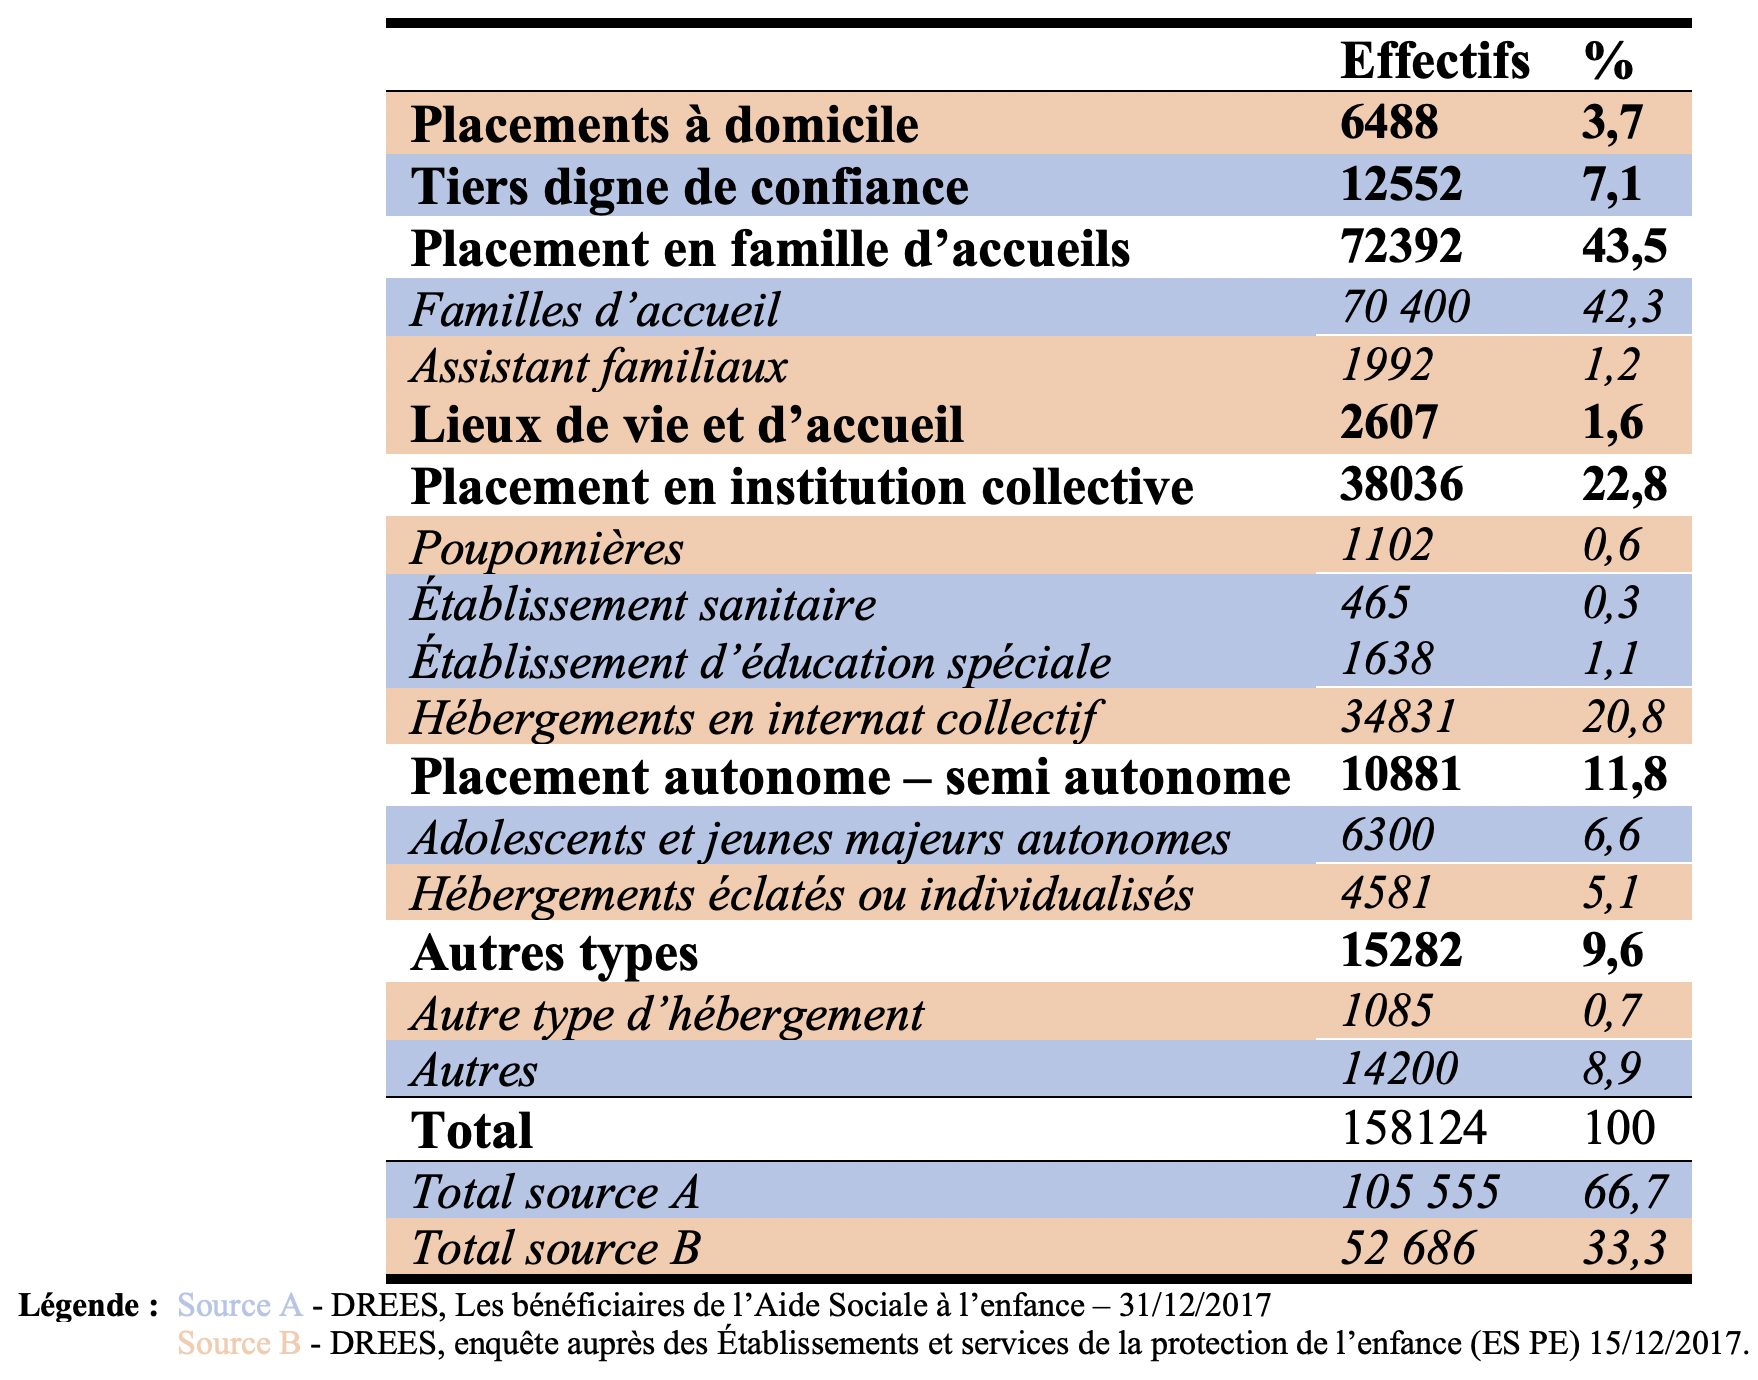
\includegraphics[width=0.8\linewidth]{Figure/Tabrep} 

}

\caption{Les champs de l'enquête sur les bénéficiaires de l'Aide sociale à l'enfance et de l'enquête ES-PE}\label{fig:unnamed-chunk-10}
\end{figure}

On observe ainsi que seuls 33,3\% des enfants placés en Protection de
l'enfance sont présents dans l'enquête ES-PE. En effet, les familles
d'accueil représentent plus de 40\% des placements, or elles ne sont pas
présentes dans les données de l'enquête ES-PE 2017. Néanmoins, on saisit
mieux à l'aube de ces informations la portée de l'enquête ES-PE et son
positionnement dans le champ des enquêtes sur la Protection de
l'enfance, ce qui permet de comprendre tout son intérêt. En effet, cette
enquête est la seule source qui apporte autant d'informations sur ces
33,3\% d'enfants placés. Elle est aussi la seule enquête qui produit des
données à l'échelle nationale sur les établissements d'accueil de l'Aide
sociale à l'enfance et donc qui collecte des informations autant sur les
professionnels de ce secteur, que sur les enfants qui y sont protégés.

Ainsi, l'enquête ES-PE s'inscrit dans un champ de production de données
sur la Protection de l'enfance fragmenté, qui offre le plus souvent des
informations parcellaires sur différents types d'enfants et qui le plus
souvent produit essentiellement des données à visée gestionnaire rendant
difficile leur utilisation pour la production de connaissance sur ce
type de population. Cette source apparaît ainsi d'autant plus pertinente
dans toutes les informations qu'elle récolte puisqu'elles permettent
l'étude scientifique, et ce surtout en attente des données du dispositif
OLINPE. Il convient néanmoins de bien spécifier le champ que couvre
cette enquête et ses limites qui nous le verront entrave tout de même
grandement la recherche scientifique.

\hypertarget{lenquuxeate-es-pe-pruxe9sentation-et-limites}{%
\subsection{L'enquête ES-PE : présentation et
limites}\label{lenquuxeate-es-pe-pruxe9sentation-et-limites}}

\begin{quote}
\emph{Une enquête dédiée aux établissements sociaux}
\end{quote}

L'enquête ES-PE sur laquelle se concentre cette étude a été administrée
via un questionnaire en ligne au premier semestre 2018 et porte sur
l'année 2017. Plus précisément, l'activité et les enfants présents sont
ceux au 15 décembre 2017, alors que le personnel est celui en date du 31
décembre 2017 et que les enfants sortis sont ceux au cours de l'année
2017. Le champ de l'enquête est celui des établissements de placement
civil et pénal dans lesquels on retrouve des enfants placés par le juge
ou l'aide sociale à l'enfance (ASE) ou suivis par la protection
judiciaire de la jeunesse (PJJ). L'enquête est menée à l'échelle de la
France métropolitaine et des DOM-TOM, hors Mayotte.

\mdfsetup{%
middlelinewidth=2pt,
backgroundcolor=gray!10,
roundcorner=10pt}
\begin{mdframed}[frametitle=Le champ retenu pour notre étude]

Pour notre étude, du fait de l’hétérogénéité des publics accueillis et bien que notre regard se porte particulièrement sur les maisons d’enfants à caractère social, nous avons plus globalement choisi de nous restreindre aux établissements relevant de l’Aide sociale à l’enfance pour d’éventuelles comparaisons : les pouponnières à caractère social, les foyers de l’enfance, les lieux de vie et d’accueil, les villages d’enfants. En effet, les autres types d’établissements présents dans l’enquête ES-PE 2017, relèvent de la protection judiciaire de la jeunesse (PJJ) et les centres associatifs de placement familial socio-éducatif et concernent un type encore différent de population. Les informations portant sur les mesures d’action éducative (AED et AEMO) et sur les clubs de prévention spécialisée ont été aussi écartées, étant donné que nous nous concentrons sur les jeunes étant accueillis en hébergement dans un établissement. L’accueil mères-enfants a aussi été écarté, bien qu’il n’apparaisse que dans les données concernant l’activité des établissements. Les enfants ou jeunes accueillis chez un assistant familial et dont le placement est géré et rémunéré par un établissement sont inclus dans notre champ. 

\end{mdframed}

Pour réaliser son enquête, la DREES a utilisé le Fichier national des
établissements sanitaires (FINESS) qui répertorie toutes les structures
des domaines sanitaire, médico-social et social comme fichier de
référence. Ainsi, on y trouve l'ensemble des établissements civil
d'accueil de l'Aide sociale à l'enfance, donc les pouponnières, les
lieux de vie et d'accueil, les foyers de l'enfance, les MECS ou encore
les villages pour enfants. Le répertoire FINESS a permis à la DREES de
contacter l'ensemble de ces établissements afin qu'ils répondent à leur
enquête. En tout, 62 \% des établissements répertoriés ont
répondu\footnote{Pour des raisons d'effectifs, les tranches d'âge
  précédemment utilisées dans l'ensemble de ce mémoire n'ont pas pu être
  reprises dans ce modèle. On propose donc des tranches d'âge moins
  nombreuses qui regroupent les 0 à 10 ans ensemble. Ce choix n'est pas
  sans conséquence. En effet, nous l'avons vu les plus jeunes enfants
  sont particulièrement présents dans la classe 1 de notre CAH et pas
  dans les classes 2 et 3. Or, ces derniers se retrouvent ici englobé
  dans une catégorie bien plus large.}.

\begin{figure}

{\centering \includegraphics[width=0.8\linewidth]{Global_files/figure-latex/unnamed-chunk-11-1} 

}

\caption{Taux de réponse des différents types d'établissements de l'Aide sociale à l'enfance à l'enquête ES-PE 2017}\label{fig:unnamed-chunk-11}
\end{figure}

Tous les types d'établissements ne présentent pas le même taux de
réponse à l'enquête. Ainsi, les lieux de vie et d'accueil sont les
structures qui ont le moins répondu à l'enquête ES-PE 2017, avec 57\%
d'établissements répondants\footnote{Les effets de la variable portant
  sur le sexe des enfants placés ne sera pas présenté dans les tableaux
  suivants bien que présente en tant que variable de contrôle lors du
  calcul du modèle. Ce choix est motivé par la volonté malgré un nombre
  important de variable explicative incluses dans le modèle de présenter
  un tableau clair, mais aussi par le fait que la variable de sexe n'a
  aucun effet significatif dans ce modèle.}. Ainsi, le type
d'établissement ayant le plus haut taux de réponses est les foyers de
l'enfance à 82\%. Dans cet ensemble, les MECS affichent comparativement
un bon taux de réponse avec 71\%, ce qui permet leur bonne
représentativité dans l'enquête.

La non-réponse totale a en effet été un enjeu particulier pour la DREES
avec seulement 62\% des établissements qui ont répondu. Il est en ce
sens rassurant d'observer un bon taux de réponse pour le type
d'établissement qui occupe particulièrement notre étude. La non-réponse
totale a été gérée par la DREES à l'aide d'une pondération que nous
emploierons dans nos analyses, afin de limiter d'autant plus ce biais.

\mdfsetup{%
middlelinewidth=2pt,
backgroundcolor=gray!10,
roundcorner=10pt}
\begin{mdframed}[frametitle=La pondération dans l’enquête ES-PE 2017]

La pondération de l’enquête ES-PE 2017 a été calculée pour répondre à deux objectifs\footnote{À noter que la pondération a été calculée avec la macro Calmar sur SAS.}: augmenter la représentativité de l’échantillon et réduire le biais de non-réponse. En ce sens, ils ont construit deux pondérations en utilisant la méthode du calage sur marge. Le calage sur marge vise à redresser un échantillon en utilisant une information auxiliaire de référence. C’est-à-dire qu’on donne un poids à chaque individu pour que dans les variables catégorielles choisies, leurs effectifs soient égaux à un effectif de référence qui correspond généralement à ce qu’on observe en population totale\footnote{Olivier Sautory, « Les méthodes de calage », 2018.}. Avant de réaliser un calage sur marge prenant appui sur le répertoire FINESS, on peut choisir une des deux méthodes de gestion de la non-réponse par repondération soit avec le calage dit « direct » qui postule à partir d’un modèle de régression linéaire que le fait d’être répondant dépend des variables de calage utilisées\footnote{Thomas Deroyon, « La correction de la non-réponse par repondération », 2017.}, soit un calage après correction de la non-réponse qui vise à repondérer en première étape et se servir des poids de cette repondération pour effectuer un calage classique par la suite. Dans cette seconde méthode, on estime un modèle de régression portant sur la non-réponse et c’est à partir des probabilités de réponse estimées qu’on réalise une première pondération. C’est cette seconde méthode qui a été employée par la DREES.

À partir de ces méthodes, plusieurs pondérations ont été construites correspondant aux différentes tables de données. Comme nous travaillons sur les tables ACT, ENF et SOR, nous présentons ici leur pondération : une pour la table ACT et une autre pour les tables ENF et SOR. La première étape de gestion de la non-réponse est la même pour toutes les tables : deux régressions logistiques modélisent la non-réponse totale le premier portant sur les établissements de l’ASE avec les variables suivantes : la région, la catégorie d'établissements et la présence d'un mail dans le fichier de gestion, le second sur les établissements de la PJJ avec les variables suivantes : la catégorie d'établissements et la présence d'un mail dans le fichier de gestion.

Pour la pondération de la table ACT, le calage sur marge a été réalisé à l’aide du répertoire FINESS qui offrait par région et par catégorie d’établissements, le nombre d’établissements et les capacités d’accueil (celles déclarées pour les établissements ayant répondu, celles installées pour les non-répondants issus du répertoire FINESS). Vu que certains types d’établissements, tels que les pouponnières, les villages pour enfants ou encore les lieux de vie et d’accueil, ne sont pas assez nombreux sur le territoire, ces derniers avaient pour marges le nombre d'établissements et les capacités, par catégorie d'établissements à l’échelle nationale.

Pour la pondération des tables ENF et SOR, les marges sont les effectifs d'enfants présents dans l'établissement (déclarés dans ACT), par région, et par catégorie d'établissements pour les Foyers de l’enfance et les MECS. Pour les autres types d’établissements, le calage est le même, mais à l’échelle nationale.
\end{mdframed}

Chaque fiche du questionnaire a donné lieu à une base de données, il y
en a en tout 7, mais nous ne retenons ici que celles employées dans
notre étude : soit celle pour l'activité des établissements (ACT), celle
pour les enfants présents au 15/12/2017 (ENF) et enfin, celle pour les
enfants sortis en 2017 (SOR). Leur mise en page est dense et rappelle
les formulaires de l'administration publique. Il est à noter que les
professionnels chargés de les renseigner sont de professions variées et
sont non formés à leur remplissage. Ceci implique de probables
inégalités dans la qualité des réponses envoyées, quand bien même le
formulaire comporte de nombreuses indications afin d'aider et
d'accompagner à son remplissage.

\newpage

\begin{figure}

{\centering 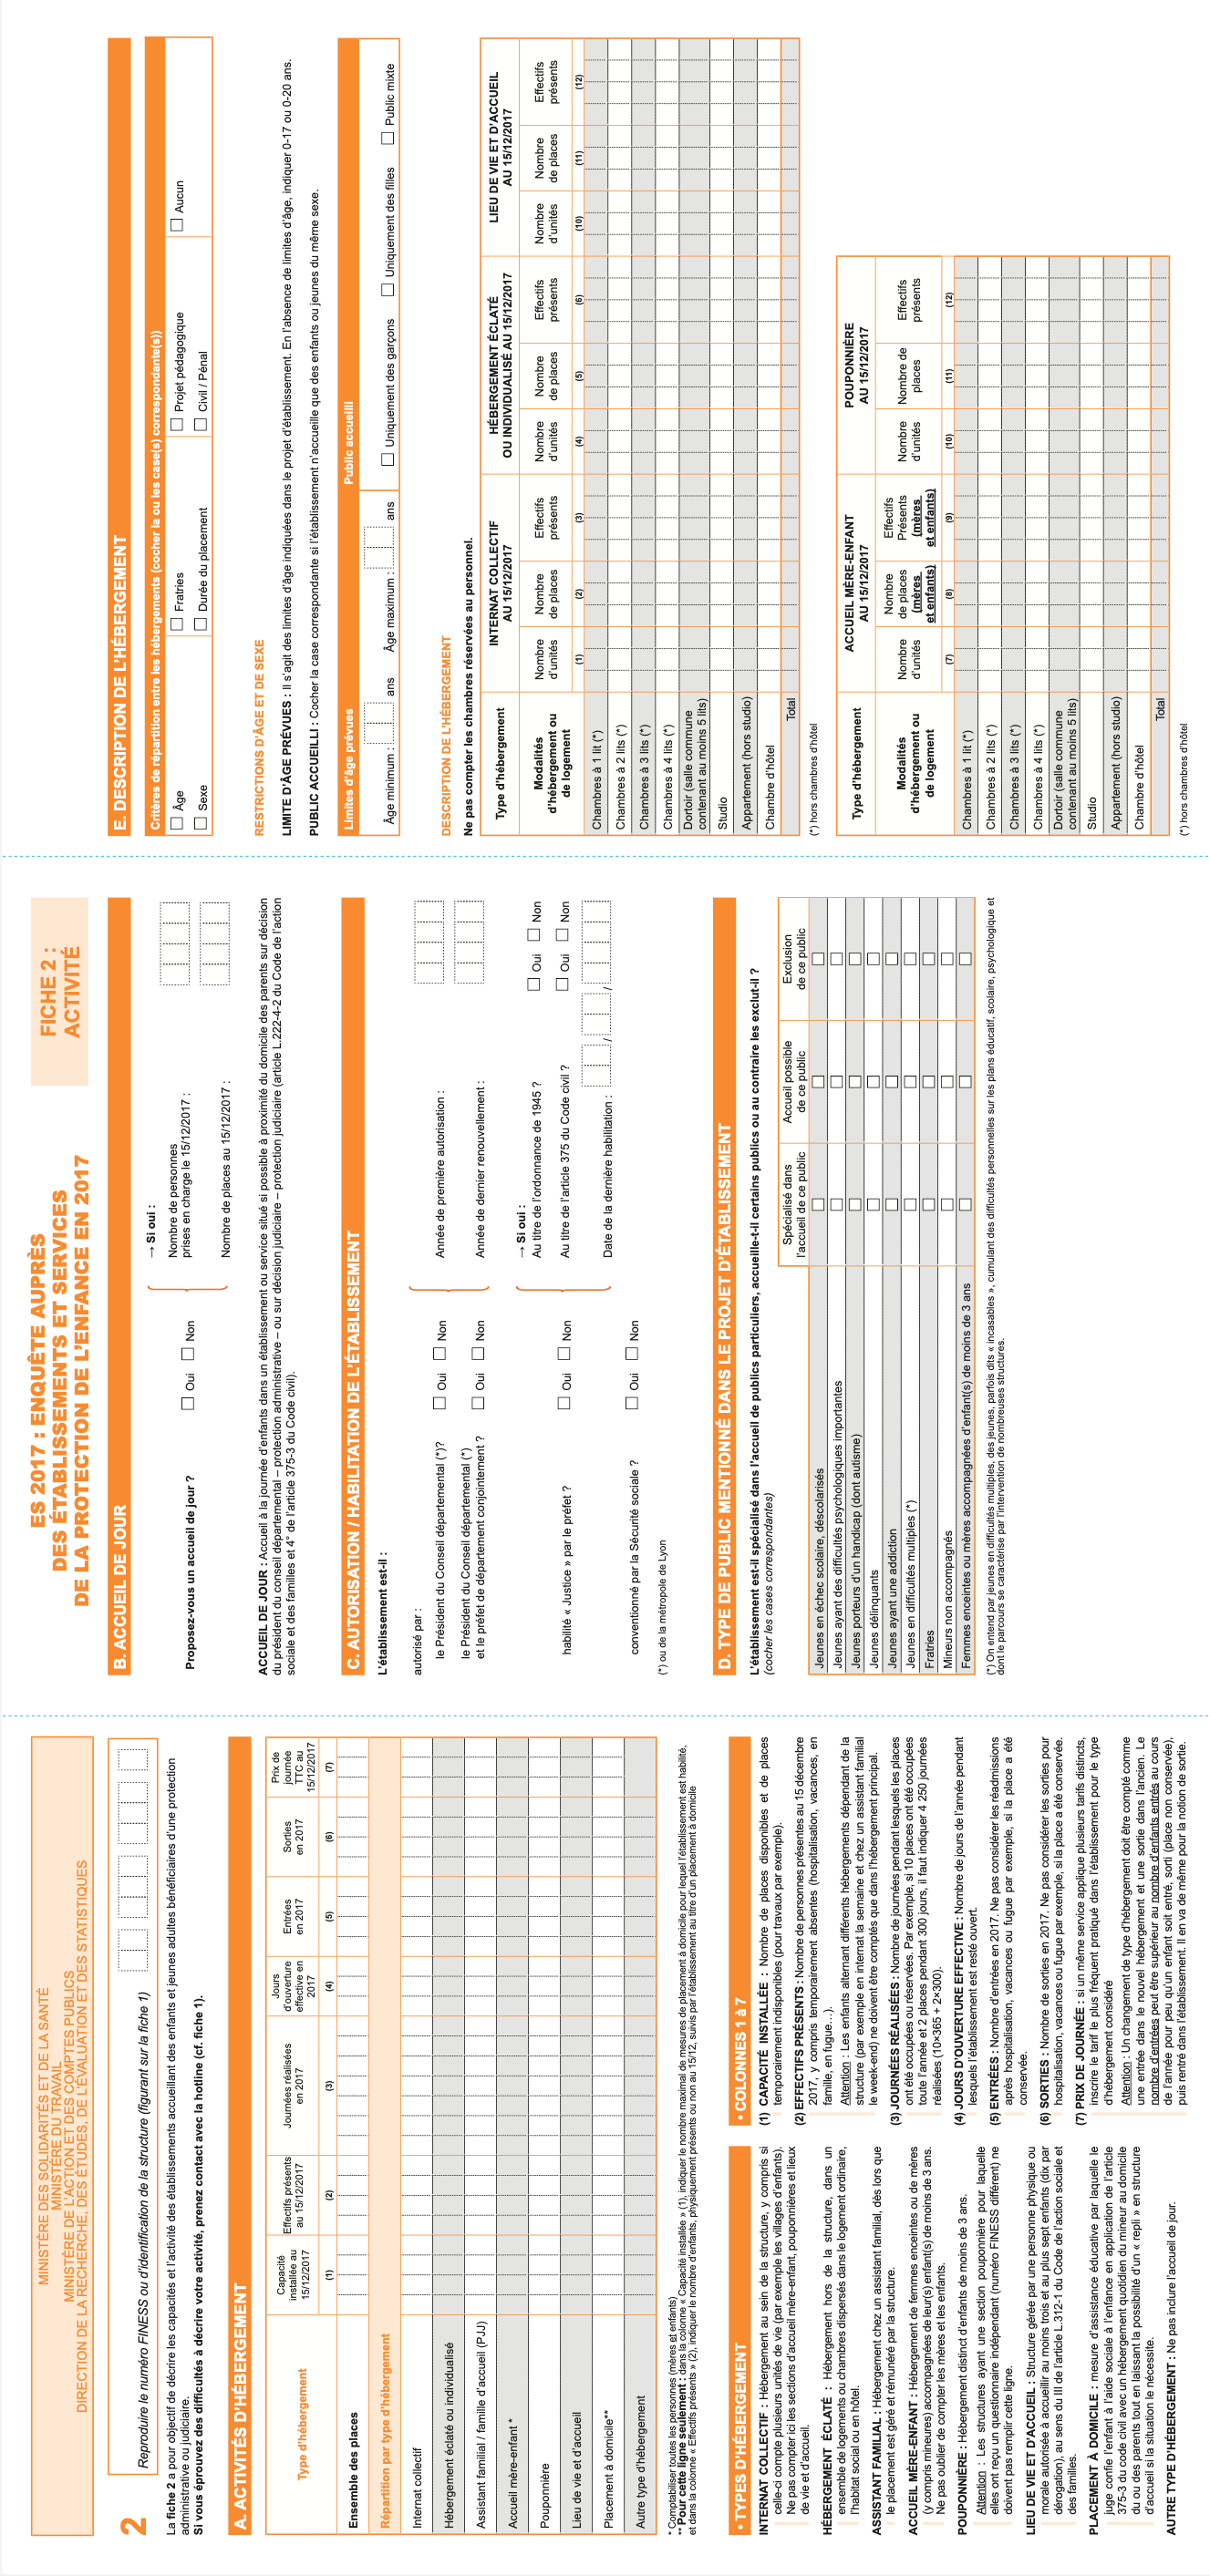
\includegraphics[width=1\linewidth]{Figure/Quest1} 

}

\caption{Exemple d’une fiche du questionnaire de l'enquête ES-PE 2017}\label{fig:unnamed-chunk-12}
\end{figure}

\begin{quote}
\emph{Les limites des données de l'enquête ES-PE 2017}
\end{quote}

Ces données comportent de nombreuses limites qu'il convient d'évoquer
avant de les utiliser dans la suite de cette étude. Avec la refonte de
leur enquête, la DREES cherchait à la fois à recueillir des données
permettant des analyses plus approfondies pour faire avancer l'état de
la connaissance sur la Protection de l'enfance, et à conserver leur
visée initiale qui est gestionnaire. Ainsi, de nombreuses séries de
questions ont été ajoutées. Pour autant, leur formulation, l'absence de
certaines questions ou le retrait d'autres afin de respecter le
règlement général sur la protection des données (RGPD), rend
particulièrement difficile la construction d'une étude. Nous proposons
ici un rapide tour des limites principales qui ont entravé notre
travail, elles sont de deux types : absence de données et données
incomplètes.

La première limite est celle de l'absence de la variable indiquant la
région de l'établissement. Nous l'avons vu avec la départementalisation,
les départements gèrent leur propre service d'aide sociale à l'enfance.
Ils appliquent ainsi des politiques différentes qui ont un effet direct
sur le type d'établissements présents sur leur territoire, leur nombre,
le type de public visé\ldots{} La prise en charge est pourtant
dépendante en partie des moyens d'interventions disponibles dans les
départements\footnote{L. Marquet, Z. Perron et I. Frechon, {«~Les
  Enfants Protégés En {France}. {Différences} Selon Les Politiques
  Départementales de Prise En Charge~»}, art cit.}. Il existe bien une
variable géographique dans les données transmises, mais elle porte sur
le département du domicile du mineur ou jeune majeur. Une information
floue donc puisqu'elle ne permet que de localiser où les parents ou
tuteurs légaux vivent, sans pouvoir retracer le département qui a mis en
place la mesure administrative ou qui doit s'occuper de l'application
d'une mesure judiciaire. Lorsque l'on se reporte sur les données de la
DREES et notamment sur l'enquête concernant les bénéficiaires de l'aide
sociale à l'enfance, on observe pourtant de véritables différences entre
les différents départements en 2017. À titre d'exemple, on voit que
certains départements tels que l'Ain ou les Hautes-Alpes placent les
enfants sous leur protection que dans un type d'établissement, et dans
le cas présent qu'en MECS. L'ONPE s'est elle aussi intéressée récemment
aux disparités départementales en matière de politique sociale de la
protection de l'enfance en liant les données de la DREES sur les
bénéficiaires de l'aide sociale à l'enfance et celles du ministère de la
Justice\footnote{ONPE, \emph{La Population Des Enfants Suivis En
  Protection de l'enfance Au 31/12/2018 : Les Disparités
  Départementales}, s.l., 2020.}. Ils ont particulièrement étudié le
taux de prise en charge par département qui correspond à la part de
mineurs ou jeunes majeurs concernés par une prestation ou mesure de
protection de l'enfance par rapport au nombre total de mineurs ou jeunes
majeurs par département. Ils constatent une importante variation de ce
taux entre les départements qui s'accentue depuis 2009. Ainsi, au 31
décembre 2018, les taux de prise en charge varient selon les
départements de 10,9 ‰\footnote{À noter qu'une version réduite de ce
  modèle est proposée dans les Annexes (voir Annexes - ).} à 44,8 ‰
concernant les mineurs et de 0,1 ‰ à 21 ‰ en ce qui concerne les jeunes
majeurs\footnote{ONPE, \emph{La Population Des Enfants Suivis En
  Protection de l'enfance Au 31/12/2018 }, \emph{op.~cit.}}. Le fait que
cette variable soit non comprise dans nos données produit une ignorance
sur un phénomène qui gagnerait à être pris en compte dans notre étude.

La deuxième limite majeure de ces données est qu'elles sont incomplètes
soit parce que des questions n'ont pas été posées aux structures, soit
parce que les modalités de réponses sont floues. En témoigne le cas
concret qui est au cœur de notre étude des questions posées sur les
types d'hébergements avant et après avoir été placé dans l'établissement
observé en 2017 dans le cas des enfants sortis au cours de l'année 2017.
Ces variables auraient pu permettre de reconstruire des trajectoires de
placement en s'intéressant particulièrement au type d'hébergement.
Néanmoins, une telle analyse est rendue impossible par l'absence de
date. En effet, la date d'entrée dans le type d'hébergement avant
l'arrivée dans l'établissement observée n'est pas demandée dans
l'enquête ES-PE. Nous avons donc l'information sur trois événements,
dont deux seulement sont datés, sachant que la fin du troisième
événement est inconnue.

\begin{longtable}[]{@{}
  >{\raggedright\arraybackslash}p{(\columnwidth - 6\tabcolsep) * \real{0.2222}}
  >{\raggedright\arraybackslash}p{(\columnwidth - 6\tabcolsep) * \real{0.2222}}
  >{\raggedright\arraybackslash}p{(\columnwidth - 6\tabcolsep) * \real{0.2222}}
  >{\raggedright\arraybackslash}p{(\columnwidth - 6\tabcolsep) * \real{0.2222}}@{}}
\caption{Les trois événements du parcours de placement présents dans
l'enquête ES-PE 2017}\tabularnewline
\toprule
\begin{minipage}[b]{\linewidth}\raggedright
\end{minipage} & \begin{minipage}[b]{\linewidth}\raggedright
\textbf{Temps -- 1 :}

juste avant l'entrée dans l ' établissement d'observation
\end{minipage} & \begin{minipage}[b]{\linewidth}\raggedright
\textbf{Temps 0 :}

observation enquête ES-PE 2017
\end{minipage} & \begin{minipage}[b]{\linewidth}\raggedright
\textbf{Temps +1 :}

à la sortie de l ' établissement observé
\end{minipage} \\
\midrule
\endfirsthead
\toprule
\begin{minipage}[b]{\linewidth}\raggedright
\end{minipage} & \begin{minipage}[b]{\linewidth}\raggedright
\textbf{Temps -- 1 :}

juste avant l'entrée dans l ' établissement d'observation
\end{minipage} & \begin{minipage}[b]{\linewidth}\raggedright
\textbf{Temps 0 :}

observation enquête ES-PE 2017
\end{minipage} & \begin{minipage}[b]{\linewidth}\raggedright
\textbf{Temps +1 :}

à la sortie de l ' établissement observé
\end{minipage} \\
\midrule
\endhead
\textbf{Variable sur le type d'héb ergement} & ARES & HEBE & SRES \\
\textbf{Élément manquant} & Sans date d'entrée & Avec date d'entrée &
Avec date de sortie, mais sans date de fin \\
\bottomrule
\end{longtable}

\rightline{\small{~Source : Enquête ES-PE 2017, DREES.}}

À ceci s'ajoute, le fait que nous avons bien la date du premier
placement de l'enfant qui peut donc correspondre ou non au type
d'hébergement avant l'entrée dans l'établissement d'observation (Temps
-1), mais aucune information complémentaire nous permettra de nous en
assurer, ou au type d'hébergement dans l'établissement d'observation
(Temps 0). Même en réduisant l'échantillon aux seuls enfants qui ont la
même date de premier placement et d'entrée dans l'établissement, cela
réduit fortement l'intérêt d'une analyse de trajectoire, puisque seuls
deux événements seront alors utilisés dont le dernier qui est le type
d'hébergement à la sortie de l'établissement d'observation (temps + 1)
qui n'a pas de date de fin\footnote{À noter qu'à titre d'essai, une
  tentative d'analyse de trajectoire a tout de même été réalisée et
  qu'elle est présente dans les annexes. Elle permet ainsi de mettre en
  lumière les difficultés relatées ici.}.

Tout ceci est renforcé par le flou des modalités des variables ARES et
SRES qui invitent à la prudence quant à l'utilisation de ces variables
dans une analyse.

\begin{longtable}[]{@{}
  >{\raggedright\arraybackslash}p{(\columnwidth - 2\tabcolsep) * \real{0.1250}}
  >{\raggedright\arraybackslash}p{(\columnwidth - 2\tabcolsep) * \real{0.8611}}@{}}
\caption{Les modalités des variables sur le type d'hébergement avant et
après le placement dans l'établissement observé (ARES et
SRES)}\tabularnewline
\toprule
\begin{minipage}[b]{\linewidth}\raggedright
\end{minipage} & \begin{minipage}[b]{\linewidth}\raggedright
\textbf{Modalités des variables ARES et SRES}
\end{minipage} \\
\midrule
\endfirsthead
\toprule
\begin{minipage}[b]{\linewidth}\raggedright
\end{minipage} & \begin{minipage}[b]{\linewidth}\raggedright
\textbf{Modalités des variables ARES et SRES}
\end{minipage} \\
\midrule
\endhead
1 & Chez les parents \\
2 & Chez de la famille, des amis, un tiers digne de confiance judiciaire
ou un tiers administratif \\
3 & Dans un logement personnel, hors logement accompagné, En logement
accompagné (FJT, résidence sociale\ldots), En centre d'hébergement
(CHRS, CADA, hébergement d'urgence\ldots), Hébergement de fortune
(baraque, squat\ldots), hébergement mobile (caravane, péniche\ldots), à
la rue \\
4 & En établissement de placement relevant du civil (MECS, foyer de
l'enfance\ldots) \\
5 & En établissement de placement relevant du pénal (centre éducatif
fermé/renforcé, établissement de placement éducatif\ldots), En
établissement pénitentiaire \\
6 & Chez un assistant familial \\
7 & En établissement médico-social (y compris handicap), En
établissement hospitalier \\
8 & Autre, Internat scolaire \\
9 & Inconnu, NA \\
\bottomrule
\end{longtable}

\rightline{\small{~Source : Enquête ES-PE 2017, DREES.}}

Par exemple, les modalités « chez les parents » ou « chez de la famille,
des amis, un tiers digne de confiance judiciaire ou un tiers
administratif » ne permettent pas de savoir si l'enfant est sorti de la
Protection de l'enfance ou s'il bénéficiait ou bénéficie encore d'une
mesure. Mais aussi, la modalité regroupant l'ensemble des types de
logements accompagnés ou non produit de l'incertitude du fait du nombre
important de situations différentes qu'elle regroupe.

Maintenant que l'enquête a été présentée et que ses limites principales
ont été évoquées, nous pouvons plus précisément étudier les populations
auxquelles elle s'intéresse. Nous l'avons dit à plusieurs reprises, le
public concerné par la protection de l'enfance est hétérogène autant
dans les situations qui conduisent au placement qu'en termes de
caractéristiques individuelles. Un autre point a aussi été évoqué, le
fait que notre enquête propose des données sur deux types principaux
d'enfants placés : les enfants présents au 15 décembre 2017 et les
enfants sortis au cours de 2017. Outre l'hétérogénéité de ces publics
qu'il convient de préciser, on peut ainsi se demander également si les
enfants présents et ceux sortis sont les mêmes où s'ils relèvent de
caractéristiques bien particulières.

\hypertarget{le-type-de-public-accueilli-en-mecs-en-2017}{%
\section{Le type de public accueilli en MECS en
2017}\label{le-type-de-public-accueilli-en-mecs-en-2017}}

\hypertarget{les-enfants-pruxe9sents-en-mecs-au-15-duxe9cembre-2017}{%
\subsection{Les enfants présents en MECS au 15 décembre
2017}\label{les-enfants-pruxe9sents-en-mecs-au-15-duxe9cembre-2017}}

Pour présenter le public accueilli en MECS, nous allons nous servir des
données aussi disponibles dans l'enquête ES-PE 2017 sur les autres types
d'établissement de placement de l'aide sociale à l'enfance. Ces derniers
vont nous servir de point de comparaison, afin de spécifier
particulièrement la population présente en MECS.

\begin{quote}
\emph{Une présence importante d'adolescents et jeunes majeurs en MECS}
\end{quote}

Ainsi, la principale caractéristique des enfants présents en MECS en
2017 est l'âge\footnote{L'âge à l'entrée dans l'établissement a été
  recodé en tranche d'âge pour permettre des analyses. Les tranches
  d'âge choisies sont celles déjà employées dans la littérature sur ces
  données et surtout sur l'étude menée par Élisa Abassi : « 61 000
  enfants, adolescents et jeunes majeurs hébergés fin 2017 dans les
  établissements de l'aide sociale à l'enfance », art cit.}. Ce type
d'établissement semble particulièrement tourné vers l'accueil d'un
public à partir de 7 ans et adolescent ou jeune majeurs à partir de 15 à
17 ans et 18 ans à plus. Cette caractéristique de l'âge les distingue
d'autres types d'établissement tels que les villages pour enfants ou les
Pouponnières. À ceci, s'ajoute un public plus masculin en MECS (à 61\%)
que dans ces deux autres types d'établissement (respectivement à 49\% et
54\% de garçons).

\begin{singlespace}
\providecommand{\docline}[3]{\noalign{\global\setlength{\arrayrulewidth}{#1}}\arrayrulecolor[HTML]{#2}\cline{#3}}

\setlength{\tabcolsep}{2pt}

\renewcommand*{\arraystretch}{1.5}

\begin{longtable}[c]{|p{1.00in}|p{1.00in}|p{1.00in}|p{1.00in}|p{1.00in}|p{1.00in}}

\caption{Les caractéristiques individuelles des enfants sortis au cours de 2017 par catégorie d\textquotesingle{}établissement (\% pondérés)
}\\

\hhline{>{\arrayrulecolor[HTML]{000000}\global\arrayrulewidth=1pt}->{\arrayrulecolor[HTML]{000000}\global\arrayrulewidth=1pt}->{\arrayrulecolor[HTML]{000000}\global\arrayrulewidth=1pt}->{\arrayrulecolor[HTML]{000000}\global\arrayrulewidth=1pt}->{\arrayrulecolor[HTML]{000000}\global\arrayrulewidth=1pt}->{\arrayrulecolor[HTML]{000000}\global\arrayrulewidth=1pt}-}

\multicolumn{1}{!{\color[HTML]{000000}\vrule width 0pt}>{\centering}p{\dimexpr 1in+0\tabcolsep+0\arrayrulewidth}}{\fontsize{11}{11}\selectfont{\textcolor[HTML]{000000}{\global\setmainfont{Times}{}}}} & \multicolumn{1}{!{\color[HTML]{000000}\vrule width 0pt}>{\centering}p{\dimexpr 1in+0\tabcolsep+0\arrayrulewidth}}{\fontsize{11}{11}\selectfont{\textcolor[HTML]{000000}{\global\setmainfont{Times}{MECS,\ N\ =\ 25525}}}} & \multicolumn{1}{!{\color[HTML]{000000}\vrule width 0pt}>{\centering}p{\dimexpr 1in+0\tabcolsep+0\arrayrulewidth}}{\fontsize{11}{11}\selectfont{\textcolor[HTML]{000000}{\global\setmainfont{Times}{Foyers,\ N\ =\ 6441}}}} & \multicolumn{1}{!{\color[HTML]{000000}\vrule width 0pt}>{\centering}p{\dimexpr 1in+0\tabcolsep+0\arrayrulewidth}}{\fontsize{11}{11}\selectfont{\textcolor[HTML]{000000}{\global\setmainfont{Times}{Lieux\ de\ vie,\ N\ =\ 1223}}}} & \multicolumn{1}{!{\color[HTML]{000000}\vrule width 0pt}>{\centering}p{\dimexpr 1in+0\tabcolsep+0\arrayrulewidth}}{\fontsize{11}{11}\selectfont{\textcolor[HTML]{000000}{\global\setmainfont{Times}{Villages,\ N\ =\ 1200}}}} & \multicolumn{1}{!{\color[HTML]{000000}\vrule width 0pt}>{\centering}p{\dimexpr 1in+0\tabcolsep+0\arrayrulewidth}!{\color[HTML]{000000}\vrule width 0pt}}{\fontsize{11}{11}\selectfont{\textcolor[HTML]{000000}{\global\setmainfont{Times}{Pouponnières,\ N\ =\ 574}}}} \\

\hhline{>{\arrayrulecolor[HTML]{000000}\global\arrayrulewidth=1pt}->{\arrayrulecolor[HTML]{000000}\global\arrayrulewidth=1pt}->{\arrayrulecolor[HTML]{000000}\global\arrayrulewidth=1pt}->{\arrayrulecolor[HTML]{000000}\global\arrayrulewidth=1pt}->{\arrayrulecolor[HTML]{000000}\global\arrayrulewidth=1pt}->{\arrayrulecolor[HTML]{000000}\global\arrayrulewidth=1pt}-}

\endfirsthead

\hhline{>{\arrayrulecolor[HTML]{000000}\global\arrayrulewidth=1pt}->{\arrayrulecolor[HTML]{000000}\global\arrayrulewidth=1pt}->{\arrayrulecolor[HTML]{000000}\global\arrayrulewidth=1pt}->{\arrayrulecolor[HTML]{000000}\global\arrayrulewidth=1pt}->{\arrayrulecolor[HTML]{000000}\global\arrayrulewidth=1pt}->{\arrayrulecolor[HTML]{000000}\global\arrayrulewidth=1pt}-}

\multicolumn{1}{!{\color[HTML]{000000}\vrule width 0pt}>{\centering}p{\dimexpr 1in+0\tabcolsep+0\arrayrulewidth}}{\fontsize{11}{11}\selectfont{\textcolor[HTML]{000000}{\global\setmainfont{Times}{}}}} & \multicolumn{1}{!{\color[HTML]{000000}\vrule width 0pt}>{\centering}p{\dimexpr 1in+0\tabcolsep+0\arrayrulewidth}}{\fontsize{11}{11}\selectfont{\textcolor[HTML]{000000}{\global\setmainfont{Times}{MECS,\ N\ =\ 25525}}}} & \multicolumn{1}{!{\color[HTML]{000000}\vrule width 0pt}>{\centering}p{\dimexpr 1in+0\tabcolsep+0\arrayrulewidth}}{\fontsize{11}{11}\selectfont{\textcolor[HTML]{000000}{\global\setmainfont{Times}{Foyers,\ N\ =\ 6441}}}} & \multicolumn{1}{!{\color[HTML]{000000}\vrule width 0pt}>{\centering}p{\dimexpr 1in+0\tabcolsep+0\arrayrulewidth}}{\fontsize{11}{11}\selectfont{\textcolor[HTML]{000000}{\global\setmainfont{Times}{Lieux\ de\ vie,\ N\ =\ 1223}}}} & \multicolumn{1}{!{\color[HTML]{000000}\vrule width 0pt}>{\centering}p{\dimexpr 1in+0\tabcolsep+0\arrayrulewidth}}{\fontsize{11}{11}\selectfont{\textcolor[HTML]{000000}{\global\setmainfont{Times}{Villages,\ N\ =\ 1200}}}} & \multicolumn{1}{!{\color[HTML]{000000}\vrule width 0pt}>{\centering}p{\dimexpr 1in+0\tabcolsep+0\arrayrulewidth}!{\color[HTML]{000000}\vrule width 0pt}}{\fontsize{11}{11}\selectfont{\textcolor[HTML]{000000}{\global\setmainfont{Times}{Pouponnières,\ N\ =\ 574}}}} \\

\hhline{>{\arrayrulecolor[HTML]{000000}\global\arrayrulewidth=1pt}->{\arrayrulecolor[HTML]{000000}\global\arrayrulewidth=1pt}->{\arrayrulecolor[HTML]{000000}\global\arrayrulewidth=1pt}->{\arrayrulecolor[HTML]{000000}\global\arrayrulewidth=1pt}->{\arrayrulecolor[HTML]{000000}\global\arrayrulewidth=1pt}->{\arrayrulecolor[HTML]{000000}\global\arrayrulewidth=1pt}-}\endhead



\multicolumn{6}{!{\color[HTML]{FFFFFF}\vrule width 0pt}>{\raggedleft}p{\dimexpr 6in+10\tabcolsep+5\arrayrulewidth}!{\color[HTML]{FFFFFF}\vrule width 0pt}}{\fontsize{9}{9}\selectfont{\textcolor[HTML]{000000}{\global\setmainfont{Times}{Source\ :\ ES-PE\ 2017,\ DREES.\linebreak \ \ \ \ \ \ \ \ \ \ \ \ \ \ \ \ \ \ \ Champ\ :\ France\ entière,\ hors\ Mayotte,\ enfants\ sortis\ de\ l’établissement\ d’observation\ au\ cours\ de\ 2017\ (hors\ sections\ d'accueil\ mère-enfant).\linebreak \ \ \ \ \ \ \ \ \ \ \ \ \ \ \ \ \ \ \ Lecture\ :\ Parmi\ les\ enfants\ sortis\ au\ cours\ de\ 2017\ de\ MECS,\ on\ observe\ que\ 13\%\ d’entre\ eux\ ont\ 18\ ans\ à\ plus,\ contre\ seulement\ 5\%\ des\ enfants\ sortis\ des\ foyers\ de\ l’enfance}}}} \\

\endfoot



\multicolumn{1}{!{\color[HTML]{000000}\vrule width 0pt}>{\centering}p{\dimexpr 1in+0\tabcolsep+0\arrayrulewidth}}{\fontsize{10}{10}\selectfont{\textcolor[HTML]{000000}{\global\setmainfont{Times}{Sexe}}}} & \multicolumn{1}{!{\color[HTML]{000000}\vrule width 0pt}>{\centering}p{\dimexpr 1in+0\tabcolsep+0\arrayrulewidth}}{\fontsize{10}{10}\selectfont{\textcolor[HTML]{000000}{\global\setmainfont{Times}{}}}} & \multicolumn{1}{!{\color[HTML]{000000}\vrule width 0pt}>{\centering}p{\dimexpr 1in+0\tabcolsep+0\arrayrulewidth}}{\fontsize{10}{10}\selectfont{\textcolor[HTML]{000000}{\global\setmainfont{Times}{}}}} & \multicolumn{1}{!{\color[HTML]{000000}\vrule width 0pt}>{\centering}p{\dimexpr 1in+0\tabcolsep+0\arrayrulewidth}}{\fontsize{10}{10}\selectfont{\textcolor[HTML]{000000}{\global\setmainfont{Times}{}}}} & \multicolumn{1}{!{\color[HTML]{000000}\vrule width 0pt}>{\centering}p{\dimexpr 1in+0\tabcolsep+0\arrayrulewidth}}{\fontsize{10}{10}\selectfont{\textcolor[HTML]{000000}{\global\setmainfont{Times}{}}}} & \multicolumn{1}{!{\color[HTML]{000000}\vrule width 0pt}>{\centering}p{\dimexpr 1in+0\tabcolsep+0\arrayrulewidth}!{\color[HTML]{000000}\vrule width 0pt}}{\fontsize{10}{10}\selectfont{\textcolor[HTML]{000000}{\global\setmainfont{Times}{}}}} \\





\multicolumn{1}{!{\color[HTML]{000000}\vrule width 0pt}>{\centering}p{\dimexpr 1in+0\tabcolsep+0\arrayrulewidth}}{\fontsize{10}{10}\selectfont{\textcolor[HTML]{000000}{\global\setmainfont{Times}{Femme}}}} & \multicolumn{1}{!{\color[HTML]{000000}\vrule width 0pt}>{\centering}p{\dimexpr 1in+0\tabcolsep+0\arrayrulewidth}}{\fontsize{10}{10}\selectfont{\textcolor[HTML]{000000}{\global\setmainfont{Times}{39}}}} & \multicolumn{1}{!{\color[HTML]{000000}\vrule width 0pt}>{\centering}p{\dimexpr 1in+0\tabcolsep+0\arrayrulewidth}}{\fontsize{10}{10}\selectfont{\textcolor[HTML]{000000}{\global\setmainfont{Times}{34}}}} & \multicolumn{1}{!{\color[HTML]{000000}\vrule width 0pt}>{\centering}p{\dimexpr 1in+0\tabcolsep+0\arrayrulewidth}}{\fontsize{10}{10}\selectfont{\textcolor[HTML]{000000}{\global\setmainfont{Times}{36}}}} & \multicolumn{1}{!{\color[HTML]{000000}\vrule width 0pt}>{\centering}p{\dimexpr 1in+0\tabcolsep+0\arrayrulewidth}}{\fontsize{10}{10}\selectfont{\textcolor[HTML]{000000}{\global\setmainfont{Times}{51}}}} & \multicolumn{1}{!{\color[HTML]{000000}\vrule width 0pt}>{\centering}p{\dimexpr 1in+0\tabcolsep+0\arrayrulewidth}!{\color[HTML]{000000}\vrule width 0pt}}{\fontsize{10}{10}\selectfont{\textcolor[HTML]{000000}{\global\setmainfont{Times}{46}}}} \\





\multicolumn{1}{!{\color[HTML]{000000}\vrule width 0pt}>{\centering}p{\dimexpr 1in+0\tabcolsep+0\arrayrulewidth}}{\fontsize{10}{10}\selectfont{\textcolor[HTML]{000000}{\global\setmainfont{Times}{Homme}}}} & \multicolumn{1}{!{\color[HTML]{000000}\vrule width 0pt}>{\centering}p{\dimexpr 1in+0\tabcolsep+0\arrayrulewidth}}{\fontsize{10}{10}\selectfont{\textcolor[HTML]{000000}{\global\setmainfont{Times}{61}}}} & \multicolumn{1}{!{\color[HTML]{000000}\vrule width 0pt}>{\centering}p{\dimexpr 1in+0\tabcolsep+0\arrayrulewidth}}{\fontsize{10}{10}\selectfont{\textcolor[HTML]{000000}{\global\setmainfont{Times}{66}}}} & \multicolumn{1}{!{\color[HTML]{000000}\vrule width 0pt}>{\centering}p{\dimexpr 1in+0\tabcolsep+0\arrayrulewidth}}{\fontsize{10}{10}\selectfont{\textcolor[HTML]{000000}{\global\setmainfont{Times}{64}}}} & \multicolumn{1}{!{\color[HTML]{000000}\vrule width 0pt}>{\centering}p{\dimexpr 1in+0\tabcolsep+0\arrayrulewidth}}{\fontsize{10}{10}\selectfont{\textcolor[HTML]{000000}{\global\setmainfont{Times}{49}}}} & \multicolumn{1}{!{\color[HTML]{000000}\vrule width 0pt}>{\centering}p{\dimexpr 1in+0\tabcolsep+0\arrayrulewidth}!{\color[HTML]{000000}\vrule width 0pt}}{\fontsize{10}{10}\selectfont{\textcolor[HTML]{000000}{\global\setmainfont{Times}{54}}}} \\





\multicolumn{1}{!{\color[HTML]{000000}\vrule width 0pt}>{\centering}p{\dimexpr 1in+0\tabcolsep+0\arrayrulewidth}}{\fontsize{10}{10}\selectfont{\textcolor[HTML]{000000}{\global\setmainfont{Times}{Âge\ à\ l'entrée}}}} & \multicolumn{1}{!{\color[HTML]{000000}\vrule width 0pt}>{\centering}p{\dimexpr 1in+0\tabcolsep+0\arrayrulewidth}}{\fontsize{10}{10}\selectfont{\textcolor[HTML]{000000}{\global\setmainfont{Times}{}}}} & \multicolumn{1}{!{\color[HTML]{000000}\vrule width 0pt}>{\centering}p{\dimexpr 1in+0\tabcolsep+0\arrayrulewidth}}{\fontsize{10}{10}\selectfont{\textcolor[HTML]{000000}{\global\setmainfont{Times}{}}}} & \multicolumn{1}{!{\color[HTML]{000000}\vrule width 0pt}>{\centering}p{\dimexpr 1in+0\tabcolsep+0\arrayrulewidth}}{\fontsize{10}{10}\selectfont{\textcolor[HTML]{000000}{\global\setmainfont{Times}{}}}} & \multicolumn{1}{!{\color[HTML]{000000}\vrule width 0pt}>{\centering}p{\dimexpr 1in+0\tabcolsep+0\arrayrulewidth}}{\fontsize{10}{10}\selectfont{\textcolor[HTML]{000000}{\global\setmainfont{Times}{}}}} & \multicolumn{1}{!{\color[HTML]{000000}\vrule width 0pt}>{\centering}p{\dimexpr 1in+0\tabcolsep+0\arrayrulewidth}!{\color[HTML]{000000}\vrule width 0pt}}{\fontsize{10}{10}\selectfont{\textcolor[HTML]{000000}{\global\setmainfont{Times}{}}}} \\





\multicolumn{1}{!{\color[HTML]{000000}\vrule width 0pt}>{\centering}p{\dimexpr 1in+0\tabcolsep+0\arrayrulewidth}}{\fontsize{10}{10}\selectfont{\textcolor[HTML]{000000}{\global\setmainfont{Times}{0\ à\ 3\ ans}}}} & \multicolumn{1}{!{\color[HTML]{000000}\vrule width 0pt}>{\centering}p{\dimexpr 1in+0\tabcolsep+0\arrayrulewidth}}{\fontsize{10}{10}\selectfont{\textcolor[HTML]{000000}{\global\setmainfont{Times}{3,9}}}} & \multicolumn{1}{!{\color[HTML]{000000}\vrule width 0pt}>{\centering}p{\dimexpr 1in+0\tabcolsep+0\arrayrulewidth}}{\fontsize{10}{10}\selectfont{\textcolor[HTML]{000000}{\global\setmainfont{Times}{16}}}} & \multicolumn{1}{!{\color[HTML]{000000}\vrule width 0pt}>{\centering}p{\dimexpr 1in+0\tabcolsep+0\arrayrulewidth}}{\fontsize{10}{10}\selectfont{\textcolor[HTML]{000000}{\global\setmainfont{Times}{2,6}}}} & \multicolumn{1}{!{\color[HTML]{000000}\vrule width 0pt}>{\centering}p{\dimexpr 1in+0\tabcolsep+0\arrayrulewidth}}{\fontsize{10}{10}\selectfont{\textcolor[HTML]{000000}{\global\setmainfont{Times}{22}}}} & \multicolumn{1}{!{\color[HTML]{000000}\vrule width 0pt}>{\centering}p{\dimexpr 1in+0\tabcolsep+0\arrayrulewidth}!{\color[HTML]{000000}\vrule width 0pt}}{\fontsize{10}{10}\selectfont{\textcolor[HTML]{000000}{\global\setmainfont{Times}{86}}}} \\





\multicolumn{1}{!{\color[HTML]{000000}\vrule width 0pt}>{\centering}p{\dimexpr 1in+0\tabcolsep+0\arrayrulewidth}}{\fontsize{10}{10}\selectfont{\textcolor[HTML]{000000}{\global\setmainfont{Times}{4\ à\ 6\ ans}}}} & \multicolumn{1}{!{\color[HTML]{000000}\vrule width 0pt}>{\centering}p{\dimexpr 1in+0\tabcolsep+0\arrayrulewidth}}{\fontsize{10}{10}\selectfont{\textcolor[HTML]{000000}{\global\setmainfont{Times}{9,1}}}} & \multicolumn{1}{!{\color[HTML]{000000}\vrule width 0pt}>{\centering}p{\dimexpr 1in+0\tabcolsep+0\arrayrulewidth}}{\fontsize{10}{10}\selectfont{\textcolor[HTML]{000000}{\global\setmainfont{Times}{10}}}} & \multicolumn{1}{!{\color[HTML]{000000}\vrule width 0pt}>{\centering}p{\dimexpr 1in+0\tabcolsep+0\arrayrulewidth}}{\fontsize{10}{10}\selectfont{\textcolor[HTML]{000000}{\global\setmainfont{Times}{6,9}}}} & \multicolumn{1}{!{\color[HTML]{000000}\vrule width 0pt}>{\centering}p{\dimexpr 1in+0\tabcolsep+0\arrayrulewidth}}{\fontsize{10}{10}\selectfont{\textcolor[HTML]{000000}{\global\setmainfont{Times}{31}}}} & \multicolumn{1}{!{\color[HTML]{000000}\vrule width 0pt}>{\centering}p{\dimexpr 1in+0\tabcolsep+0\arrayrulewidth}!{\color[HTML]{000000}\vrule width 0pt}}{\fontsize{10}{10}\selectfont{\textcolor[HTML]{000000}{\global\setmainfont{Times}{10}}}} \\





\multicolumn{1}{!{\color[HTML]{000000}\vrule width 0pt}>{\centering}p{\dimexpr 1in+0\tabcolsep+0\arrayrulewidth}}{\fontsize{10}{10}\selectfont{\textcolor[HTML]{000000}{\global\setmainfont{Times}{7\ à\ 12\ ans}}}} & \multicolumn{1}{!{\color[HTML]{000000}\vrule width 0pt}>{\centering}p{\dimexpr 1in+0\tabcolsep+0\arrayrulewidth}}{\fontsize{10}{10}\selectfont{\textcolor[HTML]{000000}{\global\setmainfont{Times}{30}}}} & \multicolumn{1}{!{\color[HTML]{000000}\vrule width 0pt}>{\centering}p{\dimexpr 1in+0\tabcolsep+0\arrayrulewidth}}{\fontsize{10}{10}\selectfont{\textcolor[HTML]{000000}{\global\setmainfont{Times}{21}}}} & \multicolumn{1}{!{\color[HTML]{000000}\vrule width 0pt}>{\centering}p{\dimexpr 1in+0\tabcolsep+0\arrayrulewidth}}{\fontsize{10}{10}\selectfont{\textcolor[HTML]{000000}{\global\setmainfont{Times}{32}}}} & \multicolumn{1}{!{\color[HTML]{000000}\vrule width 0pt}>{\centering}p{\dimexpr 1in+0\tabcolsep+0\arrayrulewidth}}{\fontsize{10}{10}\selectfont{\textcolor[HTML]{000000}{\global\setmainfont{Times}{41}}}} & \multicolumn{1}{!{\color[HTML]{000000}\vrule width 0pt}>{\centering}p{\dimexpr 1in+0\tabcolsep+0\arrayrulewidth}!{\color[HTML]{000000}\vrule width 0pt}}{\fontsize{10}{10}\selectfont{\textcolor[HTML]{000000}{\global\setmainfont{Times}{3,0}}}} \\





\multicolumn{1}{!{\color[HTML]{000000}\vrule width 0pt}>{\centering}p{\dimexpr 1in+0\tabcolsep+0\arrayrulewidth}}{\fontsize{10}{10}\selectfont{\textcolor[HTML]{000000}{\global\setmainfont{Times}{13\ à\ 14\ ans}}}} & \multicolumn{1}{!{\color[HTML]{000000}\vrule width 0pt}>{\centering}p{\dimexpr 1in+0\tabcolsep+0\arrayrulewidth}}{\fontsize{10}{10}\selectfont{\textcolor[HTML]{000000}{\global\setmainfont{Times}{14}}}} & \multicolumn{1}{!{\color[HTML]{000000}\vrule width 0pt}>{\centering}p{\dimexpr 1in+0\tabcolsep+0\arrayrulewidth}}{\fontsize{10}{10}\selectfont{\textcolor[HTML]{000000}{\global\setmainfont{Times}{11}}}} & \multicolumn{1}{!{\color[HTML]{000000}\vrule width 0pt}>{\centering}p{\dimexpr 1in+0\tabcolsep+0\arrayrulewidth}}{\fontsize{10}{10}\selectfont{\textcolor[HTML]{000000}{\global\setmainfont{Times}{23}}}} & \multicolumn{1}{!{\color[HTML]{000000}\vrule width 0pt}>{\centering}p{\dimexpr 1in+0\tabcolsep+0\arrayrulewidth}}{\fontsize{10}{10}\selectfont{\textcolor[HTML]{000000}{\global\setmainfont{Times}{4,5}}}} & \multicolumn{1}{!{\color[HTML]{000000}\vrule width 0pt}>{\centering}p{\dimexpr 1in+0\tabcolsep+0\arrayrulewidth}!{\color[HTML]{000000}\vrule width 0pt}}{\fontsize{10}{10}\selectfont{\textcolor[HTML]{000000}{\global\setmainfont{Times}{0,5}}}} \\





\multicolumn{1}{!{\color[HTML]{000000}\vrule width 0pt}>{\centering}p{\dimexpr 1in+0\tabcolsep+0\arrayrulewidth}}{\fontsize{10}{10}\selectfont{\textcolor[HTML]{000000}{\global\setmainfont{Times}{15\ à\ 17\ ans}}}} & \multicolumn{1}{!{\color[HTML]{000000}\vrule width 0pt}>{\centering}p{\dimexpr 1in+0\tabcolsep+0\arrayrulewidth}}{\fontsize{10}{10}\selectfont{\textcolor[HTML]{000000}{\global\setmainfont{Times}{36}}}} & \multicolumn{1}{!{\color[HTML]{000000}\vrule width 0pt}>{\centering}p{\dimexpr 1in+0\tabcolsep+0\arrayrulewidth}}{\fontsize{10}{10}\selectfont{\textcolor[HTML]{000000}{\global\setmainfont{Times}{39}}}} & \multicolumn{1}{!{\color[HTML]{000000}\vrule width 0pt}>{\centering}p{\dimexpr 1in+0\tabcolsep+0\arrayrulewidth}}{\fontsize{10}{10}\selectfont{\textcolor[HTML]{000000}{\global\setmainfont{Times}{33}}}} & \multicolumn{1}{!{\color[HTML]{000000}\vrule width 0pt}>{\centering}p{\dimexpr 1in+0\tabcolsep+0\arrayrulewidth}}{\fontsize{10}{10}\selectfont{\textcolor[HTML]{000000}{\global\setmainfont{Times}{1,7}}}} & \multicolumn{1}{!{\color[HTML]{000000}\vrule width 0pt}>{\centering}p{\dimexpr 1in+0\tabcolsep+0\arrayrulewidth}!{\color[HTML]{000000}\vrule width 0pt}}{\fontsize{10}{10}\selectfont{\textcolor[HTML]{000000}{\global\setmainfont{Times}{0,3}}}} \\





\multicolumn{1}{!{\color[HTML]{000000}\vrule width 0pt}>{\centering}p{\dimexpr 1in+0\tabcolsep+0\arrayrulewidth}}{\fontsize{10}{10}\selectfont{\textcolor[HTML]{000000}{\global\setmainfont{Times}{18\ ans\ à\ plus}}}} & \multicolumn{1}{!{\color[HTML]{000000}\vrule width 0pt}>{\centering}p{\dimexpr 1in+0\tabcolsep+0\arrayrulewidth}}{\fontsize{10}{10}\selectfont{\textcolor[HTML]{000000}{\global\setmainfont{Times}{7,1}}}} & \multicolumn{1}{!{\color[HTML]{000000}\vrule width 0pt}>{\centering}p{\dimexpr 1in+0\tabcolsep+0\arrayrulewidth}}{\fontsize{10}{10}\selectfont{\textcolor[HTML]{000000}{\global\setmainfont{Times}{2,0}}}} & \multicolumn{1}{!{\color[HTML]{000000}\vrule width 0pt}>{\centering}p{\dimexpr 1in+0\tabcolsep+0\arrayrulewidth}}{\fontsize{10}{10}\selectfont{\textcolor[HTML]{000000}{\global\setmainfont{Times}{2,6}}}} & \multicolumn{1}{!{\color[HTML]{000000}\vrule width 0pt}>{\centering}p{\dimexpr 1in+0\tabcolsep+0\arrayrulewidth}}{\fontsize{10}{10}\selectfont{\textcolor[HTML]{000000}{\global\setmainfont{Times}{0}}}} & \multicolumn{1}{!{\color[HTML]{000000}\vrule width 0pt}>{\centering}p{\dimexpr 1in+0\tabcolsep+0\arrayrulewidth}!{\color[HTML]{000000}\vrule width 0pt}}{\fontsize{10}{10}\selectfont{\textcolor[HTML]{000000}{\global\setmainfont{Times}{0}}}} \\





\multicolumn{1}{!{\color[HTML]{000000}\vrule width 0pt}>{\centering}p{\dimexpr 1in+0\tabcolsep+0\arrayrulewidth}}{\fontsize{10}{10}\selectfont{\textcolor[HTML]{000000}{\global\setmainfont{Times}{MNA}}}} & \multicolumn{1}{!{\color[HTML]{000000}\vrule width 0pt}>{\centering}p{\dimexpr 1in+0\tabcolsep+0\arrayrulewidth}}{\fontsize{10}{10}\selectfont{\textcolor[HTML]{000000}{\global\setmainfont{Times}{18}}}} & \multicolumn{1}{!{\color[HTML]{000000}\vrule width 0pt}>{\centering}p{\dimexpr 1in+0\tabcolsep+0\arrayrulewidth}}{\fontsize{10}{10}\selectfont{\textcolor[HTML]{000000}{\global\setmainfont{Times}{28}}}} & \multicolumn{1}{!{\color[HTML]{000000}\vrule width 0pt}>{\centering}p{\dimexpr 1in+0\tabcolsep+0\arrayrulewidth}}{\fontsize{10}{10}\selectfont{\textcolor[HTML]{000000}{\global\setmainfont{Times}{10}}}} & \multicolumn{1}{!{\color[HTML]{000000}\vrule width 0pt}>{\centering}p{\dimexpr 1in+0\tabcolsep+0\arrayrulewidth}}{\fontsize{10}{10}\selectfont{\textcolor[HTML]{000000}{\global\setmainfont{Times}{0,6}}}} & \multicolumn{1}{!{\color[HTML]{000000}\vrule width 0pt}>{\centering}p{\dimexpr 1in+0\tabcolsep+0\arrayrulewidth}!{\color[HTML]{000000}\vrule width 0pt}}{\fontsize{10}{10}\selectfont{\textcolor[HTML]{000000}{\global\setmainfont{Times}{0,3}}}} \\





\multicolumn{1}{!{\color[HTML]{000000}\vrule width 0pt}>{\centering}p{\dimexpr 1in+0\tabcolsep+0\arrayrulewidth}}{\fontsize{10}{10}\selectfont{\textcolor[HTML]{000000}{\global\setmainfont{Times}{Situation\ reconnue\ de\ handicap}}}} & \multicolumn{1}{!{\color[HTML]{000000}\vrule width 0pt}>{\centering}p{\dimexpr 1in+0\tabcolsep+0\arrayrulewidth}}{\fontsize{10}{10}\selectfont{\textcolor[HTML]{000000}{\global\setmainfont{Times}{13}}}} & \multicolumn{1}{!{\color[HTML]{000000}\vrule width 0pt}>{\centering}p{\dimexpr 1in+0\tabcolsep+0\arrayrulewidth}}{\fontsize{10}{10}\selectfont{\textcolor[HTML]{000000}{\global\setmainfont{Times}{12}}}} & \multicolumn{1}{!{\color[HTML]{000000}\vrule width 0pt}>{\centering}p{\dimexpr 1in+0\tabcolsep+0\arrayrulewidth}}{\fontsize{10}{10}\selectfont{\textcolor[HTML]{000000}{\global\setmainfont{Times}{28}}}} & \multicolumn{1}{!{\color[HTML]{000000}\vrule width 0pt}>{\centering}p{\dimexpr 1in+0\tabcolsep+0\arrayrulewidth}}{\fontsize{10}{10}\selectfont{\textcolor[HTML]{000000}{\global\setmainfont{Times}{11}}}} & \multicolumn{1}{!{\color[HTML]{000000}\vrule width 0pt}>{\centering}p{\dimexpr 1in+0\tabcolsep+0\arrayrulewidth}!{\color[HTML]{000000}\vrule width 0pt}}{\fontsize{10}{10}\selectfont{\textcolor[HTML]{000000}{\global\setmainfont{Times}{4,4}}}} \\

\hhline{>{\arrayrulecolor[HTML]{000000}\global\arrayrulewidth=1pt}->{\arrayrulecolor[HTML]{000000}\global\arrayrulewidth=1pt}->{\arrayrulecolor[HTML]{000000}\global\arrayrulewidth=1pt}->{\arrayrulecolor[HTML]{000000}\global\arrayrulewidth=1pt}->{\arrayrulecolor[HTML]{000000}\global\arrayrulewidth=1pt}->{\arrayrulecolor[HTML]{000000}\global\arrayrulewidth=1pt}-}



\end{longtable}
\end{singlespace}

Le fait que le public soit plus âgé en MECS est aussi à mettre en
perspective avec la présence assez importante de mineurs non accompagnés
à 18\% qui ont tendance à demander systématiquement l'accès à un contrat
jeune majeur afin de poursuivre leur protection\footnote{I. Frechon,
  {«~Les mineurs isolés étrangers et les inégalités de prise en charge
  en protection de l'enfance en France~»}, art cit.}. Ces derniers ont
en moyenne en âge d'entrée en MECS 16 ans\footnote{Avec un écart-type de
  1.4, ce qui confirme bien qu'ils sont surtout adolescents à l'entrée
  en MECS.}. Leur présence explique aussi le déséquilibre en termes de
répartition des sexes en MECS, puisque les MNA sont à 90\% des garçons.
Ainsi, on retire les mineurs non accompagnés, la part de filles en MECS
augmente à 46\%, contre 39\% avec les mineurs non accompagnés.

Les enfants protégés ayant un handicap reconnu représentent enfin 13\%
des enfants présents en MECS. Un chiffre similaire avec d'autres types
d'établissements tels que les Foyers de l'enfance (12\%) et les villages
pour enfants (11\%). Du fait du type d'accueil très personnalisé proposé
par les lieux de vie et d'accueil, il est ainsi cohérent de retrouver
particulièrement plus d'enfants en situation de handicap dans ce type
d'accueil (28\%). La population présente en MECS est ainsi plutôt
hétérogène et se caractérise surtout par l'âge avec une présence
particulière d'adolescent et de jeunes majeurs, à expliquer en partie
par la présence de mineurs non accompagnés.

\begin{quote}
\emph{Des mesures principales reflétant cette caractéristique de l'âge}
\end{quote}

Concernant les types de mesures, on observe des différences
significatives entre les différents types d'établissements qui
confirment l'hétérogénéité du public protégé en MECS.

\mdfsetup{%
middlelinewidth=2pt,
backgroundcolor=gray!10,
roundcorner=10pt}
\begin{mdframed}[frametitle=Le recodage de la variable du type de mesures (MES)]

La variable MES proposait à l’origine 19 modalités qui ont été regroupées en 7 : 
-   mesure administrative de mineur comprenant : l’accueil provisoire de mineurs (AP)
-   mesure administrative de jeune majeur comprenant : mesure de jeunes majeures (dont accueil provisoire de jeunes)
-   judiciaire confié comprenant : placement à l’ASE par le juge des enfants
-   judiciaire direct juge comprenant : Placement direct par le juge au sein d'un établissement ou d'un service au titre de l’enfance en danger ou au sein d'un établissement ou d'un service au titre de la protection des jeunes ou auprès d'un tiers digne de confiance et le placement post et pré-sentenciel
-   milieu ouvert comprenant : l’AEMO, l’AED et les mesures pénales de milieu ouvert
-   mesure touchant la responsabilité parentale comprenant : l’accueil d’urgence, la délégation de l’autorité parentale à l’ASE, à un particulier ou à un établissement, la tutelle déférée à l’ASE et enfin le retrait partiel de l’autorité parentale 
-   Autre comprenant : autre mesure et aucune mesure.

\end{mdframed}

\begin{singlespace}
\providecommand{\docline}[3]{\noalign{\global\setlength{\arrayrulewidth}{#1}}\arrayrulecolor[HTML]{#2}\cline{#3}}

\setlength{\tabcolsep}{2pt}

\renewcommand*{\arraystretch}{1.5}

\begin{longtable}[c]{|p{1.00in}|p{1.00in}|p{1.00in}|p{1.00in}|p{1.00in}|p{1.00in}}

\caption{Les types de mesures principales de placement en fonction des types d\textquotesingle{}établissements
}\\

\hhline{>{\arrayrulecolor[HTML]{000000}\global\arrayrulewidth=1pt}->{\arrayrulecolor[HTML]{000000}\global\arrayrulewidth=1pt}->{\arrayrulecolor[HTML]{000000}\global\arrayrulewidth=1pt}->{\arrayrulecolor[HTML]{000000}\global\arrayrulewidth=1pt}->{\arrayrulecolor[HTML]{000000}\global\arrayrulewidth=1pt}->{\arrayrulecolor[HTML]{000000}\global\arrayrulewidth=1pt}-}

\multicolumn{1}{!{\color[HTML]{000000}\vrule width 0pt}>{\centering}p{\dimexpr 1in+0\tabcolsep+0\arrayrulewidth}}{\fontsize{11}{11}\selectfont{\textcolor[HTML]{000000}{\global\setmainfont{Times}{}}}} & \multicolumn{1}{!{\color[HTML]{000000}\vrule width 0pt}>{\centering}p{\dimexpr 1in+0\tabcolsep+0\arrayrulewidth}}{\fontsize{11}{11}\selectfont{\textcolor[HTML]{000000}{\global\setmainfont{Times}{MECS,\ N\ =\ 25525}}}} & \multicolumn{1}{!{\color[HTML]{000000}\vrule width 0pt}>{\centering}p{\dimexpr 1in+0\tabcolsep+0\arrayrulewidth}}{\fontsize{11}{11}\selectfont{\textcolor[HTML]{000000}{\global\setmainfont{Times}{Foyers,\ N\ =\ 6441}}}} & \multicolumn{1}{!{\color[HTML]{000000}\vrule width 0pt}>{\centering}p{\dimexpr 1in+0\tabcolsep+0\arrayrulewidth}}{\fontsize{11}{11}\selectfont{\textcolor[HTML]{000000}{\global\setmainfont{Times}{Lieux\ de\ vie,\ N\ =\ 1223}}}} & \multicolumn{1}{!{\color[HTML]{000000}\vrule width 0pt}>{\centering}p{\dimexpr 1in+0\tabcolsep+0\arrayrulewidth}}{\fontsize{11}{11}\selectfont{\textcolor[HTML]{000000}{\global\setmainfont{Times}{Villages,\ N\ =\ 1200}}}} & \multicolumn{1}{!{\color[HTML]{000000}\vrule width 0pt}>{\centering}p{\dimexpr 1in+0\tabcolsep+0\arrayrulewidth}!{\color[HTML]{000000}\vrule width 0pt}}{\fontsize{11}{11}\selectfont{\textcolor[HTML]{000000}{\global\setmainfont{Times}{Pouponnières,\ N\ =\ 574}}}} \\

\hhline{>{\arrayrulecolor[HTML]{000000}\global\arrayrulewidth=1pt}->{\arrayrulecolor[HTML]{000000}\global\arrayrulewidth=1pt}->{\arrayrulecolor[HTML]{000000}\global\arrayrulewidth=1pt}->{\arrayrulecolor[HTML]{000000}\global\arrayrulewidth=1pt}->{\arrayrulecolor[HTML]{000000}\global\arrayrulewidth=1pt}->{\arrayrulecolor[HTML]{000000}\global\arrayrulewidth=1pt}-}

\endfirsthead

\hhline{>{\arrayrulecolor[HTML]{000000}\global\arrayrulewidth=1pt}->{\arrayrulecolor[HTML]{000000}\global\arrayrulewidth=1pt}->{\arrayrulecolor[HTML]{000000}\global\arrayrulewidth=1pt}->{\arrayrulecolor[HTML]{000000}\global\arrayrulewidth=1pt}->{\arrayrulecolor[HTML]{000000}\global\arrayrulewidth=1pt}->{\arrayrulecolor[HTML]{000000}\global\arrayrulewidth=1pt}-}

\multicolumn{1}{!{\color[HTML]{000000}\vrule width 0pt}>{\centering}p{\dimexpr 1in+0\tabcolsep+0\arrayrulewidth}}{\fontsize{11}{11}\selectfont{\textcolor[HTML]{000000}{\global\setmainfont{Times}{}}}} & \multicolumn{1}{!{\color[HTML]{000000}\vrule width 0pt}>{\centering}p{\dimexpr 1in+0\tabcolsep+0\arrayrulewidth}}{\fontsize{11}{11}\selectfont{\textcolor[HTML]{000000}{\global\setmainfont{Times}{MECS,\ N\ =\ 25525}}}} & \multicolumn{1}{!{\color[HTML]{000000}\vrule width 0pt}>{\centering}p{\dimexpr 1in+0\tabcolsep+0\arrayrulewidth}}{\fontsize{11}{11}\selectfont{\textcolor[HTML]{000000}{\global\setmainfont{Times}{Foyers,\ N\ =\ 6441}}}} & \multicolumn{1}{!{\color[HTML]{000000}\vrule width 0pt}>{\centering}p{\dimexpr 1in+0\tabcolsep+0\arrayrulewidth}}{\fontsize{11}{11}\selectfont{\textcolor[HTML]{000000}{\global\setmainfont{Times}{Lieux\ de\ vie,\ N\ =\ 1223}}}} & \multicolumn{1}{!{\color[HTML]{000000}\vrule width 0pt}>{\centering}p{\dimexpr 1in+0\tabcolsep+0\arrayrulewidth}}{\fontsize{11}{11}\selectfont{\textcolor[HTML]{000000}{\global\setmainfont{Times}{Villages,\ N\ =\ 1200}}}} & \multicolumn{1}{!{\color[HTML]{000000}\vrule width 0pt}>{\centering}p{\dimexpr 1in+0\tabcolsep+0\arrayrulewidth}!{\color[HTML]{000000}\vrule width 0pt}}{\fontsize{11}{11}\selectfont{\textcolor[HTML]{000000}{\global\setmainfont{Times}{Pouponnières,\ N\ =\ 574}}}} \\

\hhline{>{\arrayrulecolor[HTML]{000000}\global\arrayrulewidth=1pt}->{\arrayrulecolor[HTML]{000000}\global\arrayrulewidth=1pt}->{\arrayrulecolor[HTML]{000000}\global\arrayrulewidth=1pt}->{\arrayrulecolor[HTML]{000000}\global\arrayrulewidth=1pt}->{\arrayrulecolor[HTML]{000000}\global\arrayrulewidth=1pt}->{\arrayrulecolor[HTML]{000000}\global\arrayrulewidth=1pt}-}\endhead



\multicolumn{6}{!{\color[HTML]{FFFFFF}\vrule width 0pt}>{\raggedleft}p{\dimexpr 6in+10\tabcolsep+5\arrayrulewidth}!{\color[HTML]{FFFFFF}\vrule width 0pt}}{\fontsize{9}{9}\selectfont{\textcolor[HTML]{000000}{\global\setmainfont{Times}{Source\ :\ ES-PE\ 2017,\ DREES.\linebreak \ \ \ \ \ \ \ \ \ \ \ \ \ \ \ \ \ \ \ Champ\ :\ France\ entière,\ hors\ Mayotte,\ enfants\ présents\ dans\ l’établissement\ d’observation\ au\ 15/12/2017\ (hors\ sections\ d'accueil\ mère-enfant).\linebreak \ \ \ \ \ \ \ \ \ \ \ \ \ \ \ \ \ \ \ Lecture\ :\ Parmi\ les\ enfants\ présents\ au\ 15/12/2017\ en\ MECS,\ on\ observe\ que\ 8,9\%\ d’entre\ eux\ sont\ concernés\ par\ une\ mesure\ administrative\ jeune\ majeur.}}}} \\

\endfoot



\multicolumn{1}{!{\color[HTML]{000000}\vrule width 0pt}>{\centering}p{\dimexpr 1in+0\tabcolsep+0\arrayrulewidth}}{\fontsize{10}{10}\selectfont{\textcolor[HTML]{000000}{\global\setmainfont{Times}{\textbf{Mesure\ principale\ de\ placement}}}}} & \multicolumn{1}{!{\color[HTML]{000000}\vrule width 0pt}>{\centering}p{\dimexpr 1in+0\tabcolsep+0\arrayrulewidth}}{\fontsize{10}{10}\selectfont{\textcolor[HTML]{000000}{\global\setmainfont{Times}{}}}} & \multicolumn{1}{!{\color[HTML]{000000}\vrule width 0pt}>{\centering}p{\dimexpr 1in+0\tabcolsep+0\arrayrulewidth}}{\fontsize{10}{10}\selectfont{\textcolor[HTML]{000000}{\global\setmainfont{Times}{}}}} & \multicolumn{1}{!{\color[HTML]{000000}\vrule width 0pt}>{\centering}p{\dimexpr 1in+0\tabcolsep+0\arrayrulewidth}}{\fontsize{10}{10}\selectfont{\textcolor[HTML]{000000}{\global\setmainfont{Times}{}}}} & \multicolumn{1}{!{\color[HTML]{000000}\vrule width 0pt}>{\centering}p{\dimexpr 1in+0\tabcolsep+0\arrayrulewidth}}{\fontsize{10}{10}\selectfont{\textcolor[HTML]{000000}{\global\setmainfont{Times}{}}}} & \multicolumn{1}{!{\color[HTML]{000000}\vrule width 0pt}>{\centering}p{\dimexpr 1in+0\tabcolsep+0\arrayrulewidth}!{\color[HTML]{000000}\vrule width 0pt}}{\fontsize{10}{10}\selectfont{\textcolor[HTML]{000000}{\global\setmainfont{Times}{}}}} \\





\multicolumn{1}{!{\color[HTML]{000000}\vrule width 0pt}>{\centering}p{\dimexpr 1in+0\tabcolsep+0\arrayrulewidth}}{\fontsize{10}{10}\selectfont{\textcolor[HTML]{000000}{\global\setmainfont{Times}{Mesure\ touchant\ la\ responsabilité\ parentale}}}} & \multicolumn{1}{!{\color[HTML]{000000}\vrule width 0pt}>{\centering}p{\dimexpr 1in+0\tabcolsep+0\arrayrulewidth}}{\fontsize{10}{10}\selectfont{\textcolor[HTML]{000000}{\global\setmainfont{Times}{6,5}}}} & \multicolumn{1}{!{\color[HTML]{000000}\vrule width 0pt}>{\centering}p{\dimexpr 1in+0\tabcolsep+0\arrayrulewidth}}{\fontsize{10}{10}\selectfont{\textcolor[HTML]{000000}{\global\setmainfont{Times}{8,5}}}} & \multicolumn{1}{!{\color[HTML]{000000}\vrule width 0pt}>{\centering}p{\dimexpr 1in+0\tabcolsep+0\arrayrulewidth}}{\fontsize{10}{10}\selectfont{\textcolor[HTML]{000000}{\global\setmainfont{Times}{6,5}}}} & \multicolumn{1}{!{\color[HTML]{000000}\vrule width 0pt}>{\centering}p{\dimexpr 1in+0\tabcolsep+0\arrayrulewidth}}{\fontsize{10}{10}\selectfont{\textcolor[HTML]{000000}{\global\setmainfont{Times}{4,0}}}} & \multicolumn{1}{!{\color[HTML]{000000}\vrule width 0pt}>{\centering}p{\dimexpr 1in+0\tabcolsep+0\arrayrulewidth}!{\color[HTML]{000000}\vrule width 0pt}}{\fontsize{10}{10}\selectfont{\textcolor[HTML]{000000}{\global\setmainfont{Times}{4,7}}}} \\





\multicolumn{1}{!{\color[HTML]{000000}\vrule width 0pt}>{\centering}p{\dimexpr 1in+0\tabcolsep+0\arrayrulewidth}}{\fontsize{10}{10}\selectfont{\textcolor[HTML]{000000}{\global\setmainfont{Times}{Mesure\ administrative\ Mineur}}}} & \multicolumn{1}{!{\color[HTML]{000000}\vrule width 0pt}>{\centering}p{\dimexpr 1in+0\tabcolsep+0\arrayrulewidth}}{\fontsize{10}{10}\selectfont{\textcolor[HTML]{000000}{\global\setmainfont{Times}{8,2}}}} & \multicolumn{1}{!{\color[HTML]{000000}\vrule width 0pt}>{\centering}p{\dimexpr 1in+0\tabcolsep+0\arrayrulewidth}}{\fontsize{10}{10}\selectfont{\textcolor[HTML]{000000}{\global\setmainfont{Times}{5,8}}}} & \multicolumn{1}{!{\color[HTML]{000000}\vrule width 0pt}>{\centering}p{\dimexpr 1in+0\tabcolsep+0\arrayrulewidth}}{\fontsize{10}{10}\selectfont{\textcolor[HTML]{000000}{\global\setmainfont{Times}{13}}}} & \multicolumn{1}{!{\color[HTML]{000000}\vrule width 0pt}>{\centering}p{\dimexpr 1in+0\tabcolsep+0\arrayrulewidth}}{\fontsize{10}{10}\selectfont{\textcolor[HTML]{000000}{\global\setmainfont{Times}{2,6}}}} & \multicolumn{1}{!{\color[HTML]{000000}\vrule width 0pt}>{\centering}p{\dimexpr 1in+0\tabcolsep+0\arrayrulewidth}!{\color[HTML]{000000}\vrule width 0pt}}{\fontsize{10}{10}\selectfont{\textcolor[HTML]{000000}{\global\setmainfont{Times}{7,3}}}} \\





\multicolumn{1}{!{\color[HTML]{000000}\vrule width 0pt}>{\centering}p{\dimexpr 1in+0\tabcolsep+0\arrayrulewidth}}{\fontsize{10}{10}\selectfont{\textcolor[HTML]{000000}{\global\setmainfont{Times}{Mesure\ administrative\ Jeune\ Majeur}}}} & \multicolumn{1}{!{\color[HTML]{000000}\vrule width 0pt}>{\centering}p{\dimexpr 1in+0\tabcolsep+0\arrayrulewidth}}{\fontsize{10}{10}\selectfont{\textcolor[HTML]{000000}{\global\setmainfont{Times}{9,1}}}} & \multicolumn{1}{!{\color[HTML]{000000}\vrule width 0pt}>{\centering}p{\dimexpr 1in+0\tabcolsep+0\arrayrulewidth}}{\fontsize{10}{10}\selectfont{\textcolor[HTML]{000000}{\global\setmainfont{Times}{1,0}}}} & \multicolumn{1}{!{\color[HTML]{000000}\vrule width 0pt}>{\centering}p{\dimexpr 1in+0\tabcolsep+0\arrayrulewidth}}{\fontsize{10}{10}\selectfont{\textcolor[HTML]{000000}{\global\setmainfont{Times}{6,5}}}} & \multicolumn{1}{!{\color[HTML]{000000}\vrule width 0pt}>{\centering}p{\dimexpr 1in+0\tabcolsep+0\arrayrulewidth}}{\fontsize{10}{10}\selectfont{\textcolor[HTML]{000000}{\global\setmainfont{Times}{0,7}}}} & \multicolumn{1}{!{\color[HTML]{000000}\vrule width 0pt}>{\centering}p{\dimexpr 1in+0\tabcolsep+0\arrayrulewidth}!{\color[HTML]{000000}\vrule width 0pt}}{\fontsize{10}{10}\selectfont{\textcolor[HTML]{000000}{\global\setmainfont{Times}{0}}}} \\





\multicolumn{1}{!{\color[HTML]{000000}\vrule width 0pt}>{\centering}p{\dimexpr 1in+0\tabcolsep+0\arrayrulewidth}}{\fontsize{10}{10}\selectfont{\textcolor[HTML]{000000}{\global\setmainfont{Times}{Judiciaire\ confié}}}} & \multicolumn{1}{!{\color[HTML]{000000}\vrule width 0pt}>{\centering}p{\dimexpr 1in+0\tabcolsep+0\arrayrulewidth}}{\fontsize{10}{10}\selectfont{\textcolor[HTML]{000000}{\global\setmainfont{Times}{69}}}} & \multicolumn{1}{!{\color[HTML]{000000}\vrule width 0pt}>{\centering}p{\dimexpr 1in+0\tabcolsep+0\arrayrulewidth}}{\fontsize{10}{10}\selectfont{\textcolor[HTML]{000000}{\global\setmainfont{Times}{64}}}} & \multicolumn{1}{!{\color[HTML]{000000}\vrule width 0pt}>{\centering}p{\dimexpr 1in+0\tabcolsep+0\arrayrulewidth}}{\fontsize{10}{10}\selectfont{\textcolor[HTML]{000000}{\global\setmainfont{Times}{66}}}} & \multicolumn{1}{!{\color[HTML]{000000}\vrule width 0pt}>{\centering}p{\dimexpr 1in+0\tabcolsep+0\arrayrulewidth}}{\fontsize{10}{10}\selectfont{\textcolor[HTML]{000000}{\global\setmainfont{Times}{84}}}} & \multicolumn{1}{!{\color[HTML]{000000}\vrule width 0pt}>{\centering}p{\dimexpr 1in+0\tabcolsep+0\arrayrulewidth}!{\color[HTML]{000000}\vrule width 0pt}}{\fontsize{10}{10}\selectfont{\textcolor[HTML]{000000}{\global\setmainfont{Times}{78}}}} \\





\multicolumn{1}{!{\color[HTML]{000000}\vrule width 0pt}>{\centering}p{\dimexpr 1in+0\tabcolsep+0\arrayrulewidth}}{\fontsize{10}{10}\selectfont{\textcolor[HTML]{000000}{\global\setmainfont{Times}{Judiciaire\ direct\ juge}}}} & \multicolumn{1}{!{\color[HTML]{000000}\vrule width 0pt}>{\centering}p{\dimexpr 1in+0\tabcolsep+0\arrayrulewidth}}{\fontsize{10}{10}\selectfont{\textcolor[HTML]{000000}{\global\setmainfont{Times}{3,6}}}} & \multicolumn{1}{!{\color[HTML]{000000}\vrule width 0pt}>{\centering}p{\dimexpr 1in+0\tabcolsep+0\arrayrulewidth}}{\fontsize{10}{10}\selectfont{\textcolor[HTML]{000000}{\global\setmainfont{Times}{16}}}} & \multicolumn{1}{!{\color[HTML]{000000}\vrule width 0pt}>{\centering}p{\dimexpr 1in+0\tabcolsep+0\arrayrulewidth}}{\fontsize{10}{10}\selectfont{\textcolor[HTML]{000000}{\global\setmainfont{Times}{5,4}}}} & \multicolumn{1}{!{\color[HTML]{000000}\vrule width 0pt}>{\centering}p{\dimexpr 1in+0\tabcolsep+0\arrayrulewidth}}{\fontsize{10}{10}\selectfont{\textcolor[HTML]{000000}{\global\setmainfont{Times}{7,9}}}} & \multicolumn{1}{!{\color[HTML]{000000}\vrule width 0pt}>{\centering}p{\dimexpr 1in+0\tabcolsep+0\arrayrulewidth}!{\color[HTML]{000000}\vrule width 0pt}}{\fontsize{10}{10}\selectfont{\textcolor[HTML]{000000}{\global\setmainfont{Times}{10}}}} \\





\multicolumn{1}{!{\color[HTML]{000000}\vrule width 0pt}>{\centering}p{\dimexpr 1in+0\tabcolsep+0\arrayrulewidth}}{\fontsize{10}{10}\selectfont{\textcolor[HTML]{000000}{\global\setmainfont{Times}{Milieu\ ouvert}}}} & \multicolumn{1}{!{\color[HTML]{000000}\vrule width 0pt}>{\centering}p{\dimexpr 1in+0\tabcolsep+0\arrayrulewidth}}{\fontsize{10}{10}\selectfont{\textcolor[HTML]{000000}{\global\setmainfont{Times}{2,6}}}} & \multicolumn{1}{!{\color[HTML]{000000}\vrule width 0pt}>{\centering}p{\dimexpr 1in+0\tabcolsep+0\arrayrulewidth}}{\fontsize{10}{10}\selectfont{\textcolor[HTML]{000000}{\global\setmainfont{Times}{1,3}}}} & \multicolumn{1}{!{\color[HTML]{000000}\vrule width 0pt}>{\centering}p{\dimexpr 1in+0\tabcolsep+0\arrayrulewidth}}{\fontsize{10}{10}\selectfont{\textcolor[HTML]{000000}{\global\setmainfont{Times}{0,5}}}} & \multicolumn{1}{!{\color[HTML]{000000}\vrule width 0pt}>{\centering}p{\dimexpr 1in+0\tabcolsep+0\arrayrulewidth}}{\fontsize{10}{10}\selectfont{\textcolor[HTML]{000000}{\global\setmainfont{Times}{0,7}}}} & \multicolumn{1}{!{\color[HTML]{000000}\vrule width 0pt}>{\centering}p{\dimexpr 1in+0\tabcolsep+0\arrayrulewidth}!{\color[HTML]{000000}\vrule width 0pt}}{\fontsize{10}{10}\selectfont{\textcolor[HTML]{000000}{\global\setmainfont{Times}{0}}}} \\





\multicolumn{1}{!{\color[HTML]{000000}\vrule width 0pt}>{\centering}p{\dimexpr 1in+0\tabcolsep+0\arrayrulewidth}}{\fontsize{10}{10}\selectfont{\textcolor[HTML]{000000}{\global\setmainfont{Times}{Autre}}}} & \multicolumn{1}{!{\color[HTML]{000000}\vrule width 0pt}>{\centering}p{\dimexpr 1in+0\tabcolsep+0\arrayrulewidth}}{\fontsize{10}{10}\selectfont{\textcolor[HTML]{000000}{\global\setmainfont{Times}{1,1}}}} & \multicolumn{1}{!{\color[HTML]{000000}\vrule width 0pt}>{\centering}p{\dimexpr 1in+0\tabcolsep+0\arrayrulewidth}}{\fontsize{10}{10}\selectfont{\textcolor[HTML]{000000}{\global\setmainfont{Times}{3,9}}}} & \multicolumn{1}{!{\color[HTML]{000000}\vrule width 0pt}>{\centering}p{\dimexpr 1in+0\tabcolsep+0\arrayrulewidth}}{\fontsize{10}{10}\selectfont{\textcolor[HTML]{000000}{\global\setmainfont{Times}{2,5}}}} & \multicolumn{1}{!{\color[HTML]{000000}\vrule width 0pt}>{\centering}p{\dimexpr 1in+0\tabcolsep+0\arrayrulewidth}}{\fontsize{10}{10}\selectfont{\textcolor[HTML]{000000}{\global\setmainfont{Times}{0}}}} & \multicolumn{1}{!{\color[HTML]{000000}\vrule width 0pt}>{\centering}p{\dimexpr 1in+0\tabcolsep+0\arrayrulewidth}!{\color[HTML]{000000}\vrule width 0pt}}{\fontsize{10}{10}\selectfont{\textcolor[HTML]{000000}{\global\setmainfont{Times}{0,2}}}} \\

\hhline{>{\arrayrulecolor[HTML]{000000}\global\arrayrulewidth=1pt}->{\arrayrulecolor[HTML]{000000}\global\arrayrulewidth=1pt}->{\arrayrulecolor[HTML]{000000}\global\arrayrulewidth=1pt}->{\arrayrulecolor[HTML]{000000}\global\arrayrulewidth=1pt}->{\arrayrulecolor[HTML]{000000}\global\arrayrulewidth=1pt}->{\arrayrulecolor[HTML]{000000}\global\arrayrulewidth=1pt}-}



\end{longtable}
\end{singlespace}

En effet, confirmant l'âge plus avancé des enfants présents en MECS du
fait de la présence notamment de mineurs non accompagnés, on retrouve un
fort taux par rapport aux autres types d'établissement de mesures
principales administratives dédiées aux jeunes majeurs (8.9\%). Les MECS
accueillent aussi fortement les mesures administratives dédiées aux
mineurs (ou accueils provisoires de mineurs) à 8\%. La mesure concernant
le plus d'enfants présents en MECS reste le judiciaire confié à 67\% qui
correspond à la décision d'un juge de placer un enfant au titre de
l'enfance en danger. Il ne s'agit pas du taux le plus haut en
comparaison avec les autres types d'établissement, mais il reste
néanmoins conséquent. Ceci est de plus à mettre en lien avec le nombre
de mesures touchant la responsabilité familiale qui délègue la tutelle
partielle ou non de l'enfant à l'ASE ou à un tuteur légal, et comprend
aussi les pupilles d'État\footnote{Les pupilles de l'État représentent
  12.7\% des mesures touchant la responsabilité familiale.}.

Connaître le type de mesures les plus présentes en MECS nous renseignent
néanmoins assez peu sur la population qui y est présente\footnote{I.
  Frechon, {«~L'impossible observation de l'enfance protégée en France
  ?~»}, art cit.}, mais permet de mettre en perspective les enjeux
autour du maintien du lien avec la famille. En effet, les mesures
judiciaires sont imposées à la famille et arrivent même parfois en
dernier recours lorsque cette dernière a refusé la mesure
administrative. Parfois même, le juge décide du retrait partiel ou non
de l'autorité parentale ce qui constitue une étape supplémentaire dans
la protection de l'enfant. Dans ce cadre-là, la question du maintien du
lien avec la famille prend une teneur particulière à la vue du nombre
d'enfants présents en MECS concernés par ce type de mesures. Il s'agit
pourtant d'une préoccupation pour les professionnels en MECS. Leur rôle
devient dès lors incontournable pour tenter de réinvestir le parent dans
la vie de l'enfant ou de maintenir les liens avec la famille tout en
étant eux-mêmes les appliquant d'une mesure imposée.

\begin{quote}
\emph{L'ancienneté des enfants présents en MECS}
\end{quote}

Concernant l'ancienneté des enfants présents au 15/12/2017 dans
l'établissement d'observation, on observe des différences importantes
entre les différents types d'établissements. L'ancienneté moyenne en
MECS est de 20 mois, sachant que 25\% des enfants présents y sont depuis
5 mois ou moins et 25\% depuis 26 mois ou plus. Ces durées se
comprennent en lien avec le type d'accueil proposé par les différents
établissements.

\begin{singlespace}
\providecommand{\docline}[3]{\noalign{\global\setlength{\arrayrulewidth}{#1}}\arrayrulecolor[HTML]{#2}\cline{#3}}

\setlength{\tabcolsep}{2pt}

\renewcommand*{\arraystretch}{1.5}

\begin{longtable}[c]{|p{1.00in}|p{1.00in}|p{1.00in}|p{1.00in}|p{1.00in}|p{1.00in}}

\caption{Ancienneté (en mois) des enfants présents fin 2017 dans l\textquotesingle{}établissement d\textquotesingle{}observation par type d\textquotesingle{}établissement
}\\

\hhline{>{\arrayrulecolor[HTML]{000000}\global\arrayrulewidth=1pt}->{\arrayrulecolor[HTML]{000000}\global\arrayrulewidth=1pt}->{\arrayrulecolor[HTML]{000000}\global\arrayrulewidth=1pt}->{\arrayrulecolor[HTML]{000000}\global\arrayrulewidth=1pt}->{\arrayrulecolor[HTML]{000000}\global\arrayrulewidth=1pt}->{\arrayrulecolor[HTML]{000000}\global\arrayrulewidth=1pt}-}

\multicolumn{1}{!{\color[HTML]{000000}\vrule width 0pt}>{\centering}p{\dimexpr 1in+0\tabcolsep+0\arrayrulewidth}}{\fontsize{11}{11}\selectfont{\textcolor[HTML]{000000}{\global\setmainfont{Times}{}}}} & \multicolumn{1}{!{\color[HTML]{000000}\vrule width 0pt}>{\centering}p{\dimexpr 1in+0\tabcolsep+0\arrayrulewidth}}{\fontsize{11}{11}\selectfont{\textcolor[HTML]{000000}{\global\setmainfont{Times}{MECS,\ N\ =\ 25525}}}} & \multicolumn{1}{!{\color[HTML]{000000}\vrule width 0pt}>{\centering}p{\dimexpr 1in+0\tabcolsep+0\arrayrulewidth}}{\fontsize{11}{11}\selectfont{\textcolor[HTML]{000000}{\global\setmainfont{Times}{Foyers,\ N\ =\ 6441}}}} & \multicolumn{1}{!{\color[HTML]{000000}\vrule width 0pt}>{\centering}p{\dimexpr 1in+0\tabcolsep+0\arrayrulewidth}}{\fontsize{11}{11}\selectfont{\textcolor[HTML]{000000}{\global\setmainfont{Times}{Lieux\ de\ vie,\ N\ =\ 1223}}}} & \multicolumn{1}{!{\color[HTML]{000000}\vrule width 0pt}>{\centering}p{\dimexpr 1in+0\tabcolsep+0\arrayrulewidth}}{\fontsize{11}{11}\selectfont{\textcolor[HTML]{000000}{\global\setmainfont{Times}{Villages,\ N\ =\ 1200}}}} & \multicolumn{1}{!{\color[HTML]{000000}\vrule width 0pt}>{\centering}p{\dimexpr 1in+0\tabcolsep+0\arrayrulewidth}!{\color[HTML]{000000}\vrule width 0pt}}{\fontsize{11}{11}\selectfont{\textcolor[HTML]{000000}{\global\setmainfont{Times}{Pouponnières,\ N\ =\ 574}}}} \\

\hhline{>{\arrayrulecolor[HTML]{000000}\global\arrayrulewidth=1pt}->{\arrayrulecolor[HTML]{000000}\global\arrayrulewidth=1pt}->{\arrayrulecolor[HTML]{000000}\global\arrayrulewidth=1pt}->{\arrayrulecolor[HTML]{000000}\global\arrayrulewidth=1pt}->{\arrayrulecolor[HTML]{000000}\global\arrayrulewidth=1pt}->{\arrayrulecolor[HTML]{000000}\global\arrayrulewidth=1pt}-}

\endfirsthead

\hhline{>{\arrayrulecolor[HTML]{000000}\global\arrayrulewidth=1pt}->{\arrayrulecolor[HTML]{000000}\global\arrayrulewidth=1pt}->{\arrayrulecolor[HTML]{000000}\global\arrayrulewidth=1pt}->{\arrayrulecolor[HTML]{000000}\global\arrayrulewidth=1pt}->{\arrayrulecolor[HTML]{000000}\global\arrayrulewidth=1pt}->{\arrayrulecolor[HTML]{000000}\global\arrayrulewidth=1pt}-}

\multicolumn{1}{!{\color[HTML]{000000}\vrule width 0pt}>{\centering}p{\dimexpr 1in+0\tabcolsep+0\arrayrulewidth}}{\fontsize{11}{11}\selectfont{\textcolor[HTML]{000000}{\global\setmainfont{Times}{}}}} & \multicolumn{1}{!{\color[HTML]{000000}\vrule width 0pt}>{\centering}p{\dimexpr 1in+0\tabcolsep+0\arrayrulewidth}}{\fontsize{11}{11}\selectfont{\textcolor[HTML]{000000}{\global\setmainfont{Times}{MECS,\ N\ =\ 25525}}}} & \multicolumn{1}{!{\color[HTML]{000000}\vrule width 0pt}>{\centering}p{\dimexpr 1in+0\tabcolsep+0\arrayrulewidth}}{\fontsize{11}{11}\selectfont{\textcolor[HTML]{000000}{\global\setmainfont{Times}{Foyers,\ N\ =\ 6441}}}} & \multicolumn{1}{!{\color[HTML]{000000}\vrule width 0pt}>{\centering}p{\dimexpr 1in+0\tabcolsep+0\arrayrulewidth}}{\fontsize{11}{11}\selectfont{\textcolor[HTML]{000000}{\global\setmainfont{Times}{Lieux\ de\ vie,\ N\ =\ 1223}}}} & \multicolumn{1}{!{\color[HTML]{000000}\vrule width 0pt}>{\centering}p{\dimexpr 1in+0\tabcolsep+0\arrayrulewidth}}{\fontsize{11}{11}\selectfont{\textcolor[HTML]{000000}{\global\setmainfont{Times}{Villages,\ N\ =\ 1200}}}} & \multicolumn{1}{!{\color[HTML]{000000}\vrule width 0pt}>{\centering}p{\dimexpr 1in+0\tabcolsep+0\arrayrulewidth}!{\color[HTML]{000000}\vrule width 0pt}}{\fontsize{11}{11}\selectfont{\textcolor[HTML]{000000}{\global\setmainfont{Times}{Pouponnières,\ N\ =\ 574}}}} \\

\hhline{>{\arrayrulecolor[HTML]{000000}\global\arrayrulewidth=1pt}->{\arrayrulecolor[HTML]{000000}\global\arrayrulewidth=1pt}->{\arrayrulecolor[HTML]{000000}\global\arrayrulewidth=1pt}->{\arrayrulecolor[HTML]{000000}\global\arrayrulewidth=1pt}->{\arrayrulecolor[HTML]{000000}\global\arrayrulewidth=1pt}->{\arrayrulecolor[HTML]{000000}\global\arrayrulewidth=1pt}-}\endhead



\multicolumn{6}{!{\color[HTML]{FFFFFF}\vrule width 0pt}>{\raggedleft}p{\dimexpr 6in+10\tabcolsep+5\arrayrulewidth}!{\color[HTML]{FFFFFF}\vrule width 0pt}}{\fontsize{9}{9}\selectfont{\textcolor[HTML]{000000}{\global\setmainfont{Times}{Source\ :\ ES-PE\ 2017,\ DREES.\linebreak \ \ \ \ \ \ \ \ \ \ \ \ \ \ \ \ \ \ \ Champ\ :\ France\ entière,\ hors\ Mayotte,\ enfants\ présents\ dans\ l’établissement\ d’observation\ au\ 15/12/2017\ (hors\ sections\ d'accueil\ mère-enfant).\linebreak \ \ \ \ \ \ \ \ \ \ \ \ \ \ \ \ \ \ \ Lecture\ :\ L’ancienneté\ moyenne\ en\ MECS\ des\ enfants\ présents\ en\ 2017\ est\ de\ 20\ mois,\ sachant\ que\ 25\%\ d’entre\ eux\ y\ sont\ depuis\ 5\ mois\ ou\ moins\ et\ 25\%\ depuis\ 26\ mois\ ou\ plus.}}}} \\

\endfoot



\multicolumn{1}{!{\color[HTML]{000000}\vrule width 0pt}>{\centering}p{\dimexpr 1in+0\tabcolsep+0\arrayrulewidth}}{\fontsize{10}{10}\selectfont{\textcolor[HTML]{000000}{\global\setmainfont{Times}{\textbf{Durée\ de\ placement}}}}} & \multicolumn{1}{!{\color[HTML]{000000}\vrule width 0pt}>{\centering}p{\dimexpr 1in+0\tabcolsep+0\arrayrulewidth}}{\fontsize{10}{10}\selectfont{\textcolor[HTML]{000000}{\global\setmainfont{Times}{Q1\ :\ 5,\ \linebreak Médiane\ :\ 12,\ \linebreak Moyenne\ :\ 20,\ \linebreak Q3\ :\ 26}}}} & \multicolumn{1}{!{\color[HTML]{000000}\vrule width 0pt}>{\centering}p{\dimexpr 1in+0\tabcolsep+0\arrayrulewidth}}{\fontsize{10}{10}\selectfont{\textcolor[HTML]{000000}{\global\setmainfont{Times}{Q1\ :\ 2,\ \linebreak Médiane\ :\ 5,\ \linebreak Moyenne\ :\ 10,\ \linebreak Q3\ :\ 11}}}} & \multicolumn{1}{!{\color[HTML]{000000}\vrule width 0pt}>{\centering}p{\dimexpr 1in+0\tabcolsep+0\arrayrulewidth}}{\fontsize{10}{10}\selectfont{\textcolor[HTML]{000000}{\global\setmainfont{Times}{Q1\ :\ 6,\ \linebreak Médiane\ :\ 17,\ \linebreak Moyenne\ :\ 26,\ \linebreak Q3\ :\ 34}}}} & \multicolumn{1}{!{\color[HTML]{000000}\vrule width 0pt}>{\centering}p{\dimexpr 1in+0\tabcolsep+0\arrayrulewidth}}{\fontsize{10}{10}\selectfont{\textcolor[HTML]{000000}{\global\setmainfont{Times}{Q1\ :\ 15,\ \linebreak Médiane\ :\ 33,\ \linebreak Moyenne\ :\ 47,\ \linebreak Q3\ :\ 72}}}} & \multicolumn{1}{!{\color[HTML]{000000}\vrule width 0pt}>{\centering}p{\dimexpr 1in+0\tabcolsep+0\arrayrulewidth}!{\color[HTML]{000000}\vrule width 0pt}}{\fontsize{10}{10}\selectfont{\textcolor[HTML]{000000}{\global\setmainfont{Times}{Q1\ :\ 2,\ \linebreak Médiane\ :\ 5,\ \linebreak Moyenne\ :\ 8,\ \linebreak Q3\ :\ 11}}}} \\

\hhline{>{\arrayrulecolor[HTML]{000000}\global\arrayrulewidth=1pt}->{\arrayrulecolor[HTML]{000000}\global\arrayrulewidth=1pt}->{\arrayrulecolor[HTML]{000000}\global\arrayrulewidth=1pt}->{\arrayrulecolor[HTML]{000000}\global\arrayrulewidth=1pt}->{\arrayrulecolor[HTML]{000000}\global\arrayrulewidth=1pt}->{\arrayrulecolor[HTML]{000000}\global\arrayrulewidth=1pt}-}



\end{longtable}
\end{singlespace}

En effet, les foyers de l'enfance sont plus destinés à un accueil
d'urgence ou avant réorientation vers un placement plus pérenne dans un
autre type d'hébergement. Ceci peut expliquer pourquoi ils ont une
moyenne basse d'ancienneté avec 10 mois et une dispersion moindre du
temps passé dans ce type d'établissement. Il en va de même pour les
pouponnières à caractère social qui sont destinées à l'accueil d'un
public allant de 0 à 3 ans. Les villages pour enfants quant à eux
accueillent sur le long terme expliquant la moyenne à 33 mois. Les
enfants présents en lieux d'accueil et de vie à l'inverse ont une
ancienneté similaire bien que supérieur à celle des enfants présents en
MECS.

\hypertarget{les-enfants-sortis-de-mecs-au-cours-de-lannuxe9e-2017}{%
\subsection{Les enfants sortis de MECS au cours de l'année
2017}\label{les-enfants-sortis-de-mecs-au-cours-de-lannuxe9e-2017}}

La population des enfants sortis au cours de l'année 2017 est similaire
à celle des enfants présents au 15/12/2017, mais avec de légères
différences qui sont à souligner. En termes d'effectifs totaux dans
l'enquête ES-PE 2017, les enfants sortis sont légèrement moins nombreux
que ceux présents (30 412 contre 34 963 enfants présents sur l'ensemble
des types d'établissements de l'Aide sociale à l'enfance interrogés). Il
est à noter que quand bien même nous parlons d'enfants sortis, cela ne
veut pas dire qu'ils ne sont plus protégés par la protection de
l'enfance, mais seulement qu'ils ont quitté l'établissement
d'observation de l'enquête ES-PE au cours de 2017.

\begin{quote}
\emph{Un effet de l'âge qui joue dans les différences entre enfants
présents et enfants sortis de MECS}
\end{quote}

Les principales différences entre ces deux populations découlent de
l'effet de l'âge : les enfants sortis correspondent à une population
plus âgée (en moyenne à l'entrée dans l'établissement d'observation, les
enfants sortis ont 14 ans, tandis que les enfants présents 13 ans). Cet
effet est logique, puisque généralement les enfants placés quittent
l'établissement une fois leur majorité acquise. Cet effet se retrouve
ainsi si on regarde par tranche d'âge d'entrée dans l'établissement
d'observation en MECS où par rapport aux enfants présents, les enfants
sortis sont plus nombreux dans les tranches d'âges les plus âgées (voir
tableau 8).

\begin{singlespace}
\providecommand{\docline}[3]{\noalign{\global\setlength{\arrayrulewidth}{#1}}\arrayrulecolor[HTML]{#2}\cline{#3}}

\setlength{\tabcolsep}{2pt}

\renewcommand*{\arraystretch}{1.5}

\begin{longtable}[c]{|p{1.00in}|p{1.00in}|p{1.00in}|p{1.00in}|p{1.00in}|p{1.00in}}

\caption{Les caractéristiques individuelles des enfants sortis au cours de 2017 par catégorie d\textquotesingle{}établissement
}\\

\hhline{>{\arrayrulecolor[HTML]{000000}\global\arrayrulewidth=1pt}->{\arrayrulecolor[HTML]{000000}\global\arrayrulewidth=1pt}->{\arrayrulecolor[HTML]{000000}\global\arrayrulewidth=1pt}->{\arrayrulecolor[HTML]{000000}\global\arrayrulewidth=1pt}->{\arrayrulecolor[HTML]{000000}\global\arrayrulewidth=1pt}->{\arrayrulecolor[HTML]{000000}\global\arrayrulewidth=1pt}-}

\multicolumn{1}{!{\color[HTML]{000000}\vrule width 0pt}>{\centering}p{\dimexpr 1in+0\tabcolsep+0\arrayrulewidth}}{\fontsize{11}{11}\selectfont{\textcolor[HTML]{000000}{\global\setmainfont{Times}{}}}} & \multicolumn{1}{!{\color[HTML]{000000}\vrule width 0pt}>{\centering}p{\dimexpr 1in+0\tabcolsep+0\arrayrulewidth}}{\fontsize{11}{11}\selectfont{\textcolor[HTML]{000000}{\global\setmainfont{Times}{MECS,\ N\ =\ 15777}}}} & \multicolumn{1}{!{\color[HTML]{000000}\vrule width 0pt}>{\centering}p{\dimexpr 1in+0\tabcolsep+0\arrayrulewidth}}{\fontsize{11}{11}\selectfont{\textcolor[HTML]{000000}{\global\setmainfont{Times}{Foyers,\ N\ =\ 12941}}}} & \multicolumn{1}{!{\color[HTML]{000000}\vrule width 0pt}>{\centering}p{\dimexpr 1in+0\tabcolsep+0\arrayrulewidth}}{\fontsize{11}{11}\selectfont{\textcolor[HTML]{000000}{\global\setmainfont{Times}{Lieux\ de\ vie,\ N\ =\ 653}}}} & \multicolumn{1}{!{\color[HTML]{000000}\vrule width 0pt}>{\centering}p{\dimexpr 1in+0\tabcolsep+0\arrayrulewidth}}{\fontsize{11}{11}\selectfont{\textcolor[HTML]{000000}{\global\setmainfont{Times}{Villages,\ N\ =\ 241}}}} & \multicolumn{1}{!{\color[HTML]{000000}\vrule width 0pt}>{\centering}p{\dimexpr 1in+0\tabcolsep+0\arrayrulewidth}!{\color[HTML]{000000}\vrule width 0pt}}{\fontsize{11}{11}\selectfont{\textcolor[HTML]{000000}{\global\setmainfont{Times}{Pouponnières,\ N\ =\ 800}}}} \\

\hhline{>{\arrayrulecolor[HTML]{000000}\global\arrayrulewidth=1pt}->{\arrayrulecolor[HTML]{000000}\global\arrayrulewidth=1pt}->{\arrayrulecolor[HTML]{000000}\global\arrayrulewidth=1pt}->{\arrayrulecolor[HTML]{000000}\global\arrayrulewidth=1pt}->{\arrayrulecolor[HTML]{000000}\global\arrayrulewidth=1pt}->{\arrayrulecolor[HTML]{000000}\global\arrayrulewidth=1pt}-}

\endfirsthead

\hhline{>{\arrayrulecolor[HTML]{000000}\global\arrayrulewidth=1pt}->{\arrayrulecolor[HTML]{000000}\global\arrayrulewidth=1pt}->{\arrayrulecolor[HTML]{000000}\global\arrayrulewidth=1pt}->{\arrayrulecolor[HTML]{000000}\global\arrayrulewidth=1pt}->{\arrayrulecolor[HTML]{000000}\global\arrayrulewidth=1pt}->{\arrayrulecolor[HTML]{000000}\global\arrayrulewidth=1pt}-}

\multicolumn{1}{!{\color[HTML]{000000}\vrule width 0pt}>{\centering}p{\dimexpr 1in+0\tabcolsep+0\arrayrulewidth}}{\fontsize{11}{11}\selectfont{\textcolor[HTML]{000000}{\global\setmainfont{Times}{}}}} & \multicolumn{1}{!{\color[HTML]{000000}\vrule width 0pt}>{\centering}p{\dimexpr 1in+0\tabcolsep+0\arrayrulewidth}}{\fontsize{11}{11}\selectfont{\textcolor[HTML]{000000}{\global\setmainfont{Times}{MECS,\ N\ =\ 15777}}}} & \multicolumn{1}{!{\color[HTML]{000000}\vrule width 0pt}>{\centering}p{\dimexpr 1in+0\tabcolsep+0\arrayrulewidth}}{\fontsize{11}{11}\selectfont{\textcolor[HTML]{000000}{\global\setmainfont{Times}{Foyers,\ N\ =\ 12941}}}} & \multicolumn{1}{!{\color[HTML]{000000}\vrule width 0pt}>{\centering}p{\dimexpr 1in+0\tabcolsep+0\arrayrulewidth}}{\fontsize{11}{11}\selectfont{\textcolor[HTML]{000000}{\global\setmainfont{Times}{Lieux\ de\ vie,\ N\ =\ 653}}}} & \multicolumn{1}{!{\color[HTML]{000000}\vrule width 0pt}>{\centering}p{\dimexpr 1in+0\tabcolsep+0\arrayrulewidth}}{\fontsize{11}{11}\selectfont{\textcolor[HTML]{000000}{\global\setmainfont{Times}{Villages,\ N\ =\ 241}}}} & \multicolumn{1}{!{\color[HTML]{000000}\vrule width 0pt}>{\centering}p{\dimexpr 1in+0\tabcolsep+0\arrayrulewidth}!{\color[HTML]{000000}\vrule width 0pt}}{\fontsize{11}{11}\selectfont{\textcolor[HTML]{000000}{\global\setmainfont{Times}{Pouponnières,\ N\ =\ 800}}}} \\

\hhline{>{\arrayrulecolor[HTML]{000000}\global\arrayrulewidth=1pt}->{\arrayrulecolor[HTML]{000000}\global\arrayrulewidth=1pt}->{\arrayrulecolor[HTML]{000000}\global\arrayrulewidth=1pt}->{\arrayrulecolor[HTML]{000000}\global\arrayrulewidth=1pt}->{\arrayrulecolor[HTML]{000000}\global\arrayrulewidth=1pt}->{\arrayrulecolor[HTML]{000000}\global\arrayrulewidth=1pt}-}\endhead



\multicolumn{6}{!{\color[HTML]{FFFFFF}\vrule width 0pt}>{\raggedleft}p{\dimexpr 6in+10\tabcolsep+5\arrayrulewidth}!{\color[HTML]{FFFFFF}\vrule width 0pt}}{\fontsize{9}{9}\selectfont{\textcolor[HTML]{000000}{\global\setmainfont{Times}{Source\ :\ ES-PE\ 2017,\ DREES.\linebreak \ \ \ \ \ \ \ \ \ \ \ \ \ \ \ \ \ \ \ Champ\ :\ France\ entière,\ hors\ Mayotte,\ enfants\ sortis\ de\ l’établissement\ d’observation\ au\ cours\ de\ 2017\ (hors\ sections\ d'accueil\ mère-enfant).\linebreak \ \ \ \ \ \ \ \ \ \ \ \ \ \ \ \ \ \ \ Lecture\ :\ Parmi\ les\ enfants\ sortis\ au\ cours\ de\ 2017\ de\ MECS,\ on\ observe\ que\ 13\%\ d’entre\ eux\ ont\ 18\ ans\ à\ plus,\ contre\ seulement\ 5\%\ des\ enfants\ sortis\ des\ foyers\ de\ l’enfance.}}}} \\

\endfoot



\multicolumn{1}{!{\color[HTML]{000000}\vrule width 0pt}>{\centering}p{\dimexpr 1in+0\tabcolsep+0\arrayrulewidth}}{\fontsize{10}{10}\selectfont{\textcolor[HTML]{000000}{\global\setmainfont{Times}{\textbf{Sexe}}}}} & \multicolumn{1}{!{\color[HTML]{000000}\vrule width 0pt}>{\centering}p{\dimexpr 1in+0\tabcolsep+0\arrayrulewidth}}{\fontsize{10}{10}\selectfont{\textcolor[HTML]{000000}{\global\setmainfont{Times}{}}}} & \multicolumn{1}{!{\color[HTML]{000000}\vrule width 0pt}>{\centering}p{\dimexpr 1in+0\tabcolsep+0\arrayrulewidth}}{\fontsize{10}{10}\selectfont{\textcolor[HTML]{000000}{\global\setmainfont{Times}{}}}} & \multicolumn{1}{!{\color[HTML]{000000}\vrule width 0pt}>{\centering}p{\dimexpr 1in+0\tabcolsep+0\arrayrulewidth}}{\fontsize{10}{10}\selectfont{\textcolor[HTML]{000000}{\global\setmainfont{Times}{}}}} & \multicolumn{1}{!{\color[HTML]{000000}\vrule width 0pt}>{\centering}p{\dimexpr 1in+0\tabcolsep+0\arrayrulewidth}}{\fontsize{10}{10}\selectfont{\textcolor[HTML]{000000}{\global\setmainfont{Times}{}}}} & \multicolumn{1}{!{\color[HTML]{000000}\vrule width 0pt}>{\centering}p{\dimexpr 1in+0\tabcolsep+0\arrayrulewidth}!{\color[HTML]{000000}\vrule width 0pt}}{\fontsize{10}{10}\selectfont{\textcolor[HTML]{000000}{\global\setmainfont{Times}{}}}} \\





\multicolumn{1}{!{\color[HTML]{000000}\vrule width 0pt}>{\centering}p{\dimexpr 1in+0\tabcolsep+0\arrayrulewidth}}{\fontsize{10}{10}\selectfont{\textcolor[HTML]{000000}{\global\setmainfont{Times}{Femme}}}} & \multicolumn{1}{!{\color[HTML]{000000}\vrule width 0pt}>{\centering}p{\dimexpr 1in+0\tabcolsep+0\arrayrulewidth}}{\fontsize{10}{10}\selectfont{\textcolor[HTML]{000000}{\global\setmainfont{Times}{38}}}} & \multicolumn{1}{!{\color[HTML]{000000}\vrule width 0pt}>{\centering}p{\dimexpr 1in+0\tabcolsep+0\arrayrulewidth}}{\fontsize{10}{10}\selectfont{\textcolor[HTML]{000000}{\global\setmainfont{Times}{31}}}} & \multicolumn{1}{!{\color[HTML]{000000}\vrule width 0pt}>{\centering}p{\dimexpr 1in+0\tabcolsep+0\arrayrulewidth}}{\fontsize{10}{10}\selectfont{\textcolor[HTML]{000000}{\global\setmainfont{Times}{28}}}} & \multicolumn{1}{!{\color[HTML]{000000}\vrule width 0pt}>{\centering}p{\dimexpr 1in+0\tabcolsep+0\arrayrulewidth}}{\fontsize{10}{10}\selectfont{\textcolor[HTML]{000000}{\global\setmainfont{Times}{51}}}} & \multicolumn{1}{!{\color[HTML]{000000}\vrule width 0pt}>{\centering}p{\dimexpr 1in+0\tabcolsep+0\arrayrulewidth}!{\color[HTML]{000000}\vrule width 0pt}}{\fontsize{10}{10}\selectfont{\textcolor[HTML]{000000}{\global\setmainfont{Times}{46}}}} \\





\multicolumn{1}{!{\color[HTML]{000000}\vrule width 0pt}>{\centering}p{\dimexpr 1in+0\tabcolsep+0\arrayrulewidth}}{\fontsize{10}{10}\selectfont{\textcolor[HTML]{000000}{\global\setmainfont{Times}{Homme}}}} & \multicolumn{1}{!{\color[HTML]{000000}\vrule width 0pt}>{\centering}p{\dimexpr 1in+0\tabcolsep+0\arrayrulewidth}}{\fontsize{10}{10}\selectfont{\textcolor[HTML]{000000}{\global\setmainfont{Times}{62}}}} & \multicolumn{1}{!{\color[HTML]{000000}\vrule width 0pt}>{\centering}p{\dimexpr 1in+0\tabcolsep+0\arrayrulewidth}}{\fontsize{10}{10}\selectfont{\textcolor[HTML]{000000}{\global\setmainfont{Times}{69}}}} & \multicolumn{1}{!{\color[HTML]{000000}\vrule width 0pt}>{\centering}p{\dimexpr 1in+0\tabcolsep+0\arrayrulewidth}}{\fontsize{10}{10}\selectfont{\textcolor[HTML]{000000}{\global\setmainfont{Times}{72}}}} & \multicolumn{1}{!{\color[HTML]{000000}\vrule width 0pt}>{\centering}p{\dimexpr 1in+0\tabcolsep+0\arrayrulewidth}}{\fontsize{10}{10}\selectfont{\textcolor[HTML]{000000}{\global\setmainfont{Times}{49}}}} & \multicolumn{1}{!{\color[HTML]{000000}\vrule width 0pt}>{\centering}p{\dimexpr 1in+0\tabcolsep+0\arrayrulewidth}!{\color[HTML]{000000}\vrule width 0pt}}{\fontsize{10}{10}\selectfont{\textcolor[HTML]{000000}{\global\setmainfont{Times}{54}}}} \\





\multicolumn{1}{!{\color[HTML]{000000}\vrule width 0pt}>{\centering}p{\dimexpr 1in+0\tabcolsep+0\arrayrulewidth}}{\fontsize{10}{10}\selectfont{\textcolor[HTML]{000000}{\global\setmainfont{Times}{\textbf{Âge\ d'entrée}}}}} & \multicolumn{1}{!{\color[HTML]{000000}\vrule width 0pt}>{\centering}p{\dimexpr 1in+0\tabcolsep+0\arrayrulewidth}}{\fontsize{10}{10}\selectfont{\textcolor[HTML]{000000}{\global\setmainfont{Times}{}}}} & \multicolumn{1}{!{\color[HTML]{000000}\vrule width 0pt}>{\centering}p{\dimexpr 1in+0\tabcolsep+0\arrayrulewidth}}{\fontsize{10}{10}\selectfont{\textcolor[HTML]{000000}{\global\setmainfont{Times}{}}}} & \multicolumn{1}{!{\color[HTML]{000000}\vrule width 0pt}>{\centering}p{\dimexpr 1in+0\tabcolsep+0\arrayrulewidth}}{\fontsize{10}{10}\selectfont{\textcolor[HTML]{000000}{\global\setmainfont{Times}{}}}} & \multicolumn{1}{!{\color[HTML]{000000}\vrule width 0pt}>{\centering}p{\dimexpr 1in+0\tabcolsep+0\arrayrulewidth}}{\fontsize{10}{10}\selectfont{\textcolor[HTML]{000000}{\global\setmainfont{Times}{}}}} & \multicolumn{1}{!{\color[HTML]{000000}\vrule width 0pt}>{\centering}p{\dimexpr 1in+0\tabcolsep+0\arrayrulewidth}!{\color[HTML]{000000}\vrule width 0pt}}{\fontsize{10}{10}\selectfont{\textcolor[HTML]{000000}{\global\setmainfont{Times}{}}}} \\





\multicolumn{1}{!{\color[HTML]{000000}\vrule width 0pt}>{\centering}p{\dimexpr 1in+0\tabcolsep+0\arrayrulewidth}}{\fontsize{10}{10}\selectfont{\textcolor[HTML]{000000}{\global\setmainfont{Times}{0\ à\ 3\ ans}}}} & \multicolumn{1}{!{\color[HTML]{000000}\vrule width 0pt}>{\centering}p{\dimexpr 1in+0\tabcolsep+0\arrayrulewidth}}{\fontsize{10}{10}\selectfont{\textcolor[HTML]{000000}{\global\setmainfont{Times}{2,2}}}} & \multicolumn{1}{!{\color[HTML]{000000}\vrule width 0pt}>{\centering}p{\dimexpr 1in+0\tabcolsep+0\arrayrulewidth}}{\fontsize{10}{10}\selectfont{\textcolor[HTML]{000000}{\global\setmainfont{Times}{9,1}}}} & \multicolumn{1}{!{\color[HTML]{000000}\vrule width 0pt}>{\centering}p{\dimexpr 1in+0\tabcolsep+0\arrayrulewidth}}{\fontsize{10}{10}\selectfont{\textcolor[HTML]{000000}{\global\setmainfont{Times}{1,6}}}} & \multicolumn{1}{!{\color[HTML]{000000}\vrule width 0pt}>{\centering}p{\dimexpr 1in+0\tabcolsep+0\arrayrulewidth}}{\fontsize{10}{10}\selectfont{\textcolor[HTML]{000000}{\global\setmainfont{Times}{13}}}} & \multicolumn{1}{!{\color[HTML]{000000}\vrule width 0pt}>{\centering}p{\dimexpr 1in+0\tabcolsep+0\arrayrulewidth}!{\color[HTML]{000000}\vrule width 0pt}}{\fontsize{10}{10}\selectfont{\textcolor[HTML]{000000}{\global\setmainfont{Times}{83}}}} \\





\multicolumn{1}{!{\color[HTML]{000000}\vrule width 0pt}>{\centering}p{\dimexpr 1in+0\tabcolsep+0\arrayrulewidth}}{\fontsize{10}{10}\selectfont{\textcolor[HTML]{000000}{\global\setmainfont{Times}{4\ à\ 6\ ans}}}} & \multicolumn{1}{!{\color[HTML]{000000}\vrule width 0pt}>{\centering}p{\dimexpr 1in+0\tabcolsep+0\arrayrulewidth}}{\fontsize{10}{10}\selectfont{\textcolor[HTML]{000000}{\global\setmainfont{Times}{5,1}}}} & \multicolumn{1}{!{\color[HTML]{000000}\vrule width 0pt}>{\centering}p{\dimexpr 1in+0\tabcolsep+0\arrayrulewidth}}{\fontsize{10}{10}\selectfont{\textcolor[HTML]{000000}{\global\setmainfont{Times}{5,5}}}} & \multicolumn{1}{!{\color[HTML]{000000}\vrule width 0pt}>{\centering}p{\dimexpr 1in+0\tabcolsep+0\arrayrulewidth}}{\fontsize{10}{10}\selectfont{\textcolor[HTML]{000000}{\global\setmainfont{Times}{2,1}}}} & \multicolumn{1}{!{\color[HTML]{000000}\vrule width 0pt}>{\centering}p{\dimexpr 1in+0\tabcolsep+0\arrayrulewidth}}{\fontsize{10}{10}\selectfont{\textcolor[HTML]{000000}{\global\setmainfont{Times}{25}}}} & \multicolumn{1}{!{\color[HTML]{000000}\vrule width 0pt}>{\centering}p{\dimexpr 1in+0\tabcolsep+0\arrayrulewidth}!{\color[HTML]{000000}\vrule width 0pt}}{\fontsize{10}{10}\selectfont{\textcolor[HTML]{000000}{\global\setmainfont{Times}{11}}}} \\





\multicolumn{1}{!{\color[HTML]{000000}\vrule width 0pt}>{\centering}p{\dimexpr 1in+0\tabcolsep+0\arrayrulewidth}}{\fontsize{10}{10}\selectfont{\textcolor[HTML]{000000}{\global\setmainfont{Times}{7\ à\ 12\ ans}}}} & \multicolumn{1}{!{\color[HTML]{000000}\vrule width 0pt}>{\centering}p{\dimexpr 1in+0\tabcolsep+0\arrayrulewidth}}{\fontsize{10}{10}\selectfont{\textcolor[HTML]{000000}{\global\setmainfont{Times}{18}}}} & \multicolumn{1}{!{\color[HTML]{000000}\vrule width 0pt}>{\centering}p{\dimexpr 1in+0\tabcolsep+0\arrayrulewidth}}{\fontsize{10}{10}\selectfont{\textcolor[HTML]{000000}{\global\setmainfont{Times}{14}}}} & \multicolumn{1}{!{\color[HTML]{000000}\vrule width 0pt}>{\centering}p{\dimexpr 1in+0\tabcolsep+0\arrayrulewidth}}{\fontsize{10}{10}\selectfont{\textcolor[HTML]{000000}{\global\setmainfont{Times}{16}}}} & \multicolumn{1}{!{\color[HTML]{000000}\vrule width 0pt}>{\centering}p{\dimexpr 1in+0\tabcolsep+0\arrayrulewidth}}{\fontsize{10}{10}\selectfont{\textcolor[HTML]{000000}{\global\setmainfont{Times}{52}}}} & \multicolumn{1}{!{\color[HTML]{000000}\vrule width 0pt}>{\centering}p{\dimexpr 1in+0\tabcolsep+0\arrayrulewidth}!{\color[HTML]{000000}\vrule width 0pt}}{\fontsize{10}{10}\selectfont{\textcolor[HTML]{000000}{\global\setmainfont{Times}{3,4}}}} \\





\multicolumn{1}{!{\color[HTML]{000000}\vrule width 0pt}>{\centering}p{\dimexpr 1in+0\tabcolsep+0\arrayrulewidth}}{\fontsize{10}{10}\selectfont{\textcolor[HTML]{000000}{\global\setmainfont{Times}{13\ à\ 14\ ans}}}} & \multicolumn{1}{!{\color[HTML]{000000}\vrule width 0pt}>{\centering}p{\dimexpr 1in+0\tabcolsep+0\arrayrulewidth}}{\fontsize{10}{10}\selectfont{\textcolor[HTML]{000000}{\global\setmainfont{Times}{14}}}} & \multicolumn{1}{!{\color[HTML]{000000}\vrule width 0pt}>{\centering}p{\dimexpr 1in+0\tabcolsep+0\arrayrulewidth}}{\fontsize{10}{10}\selectfont{\textcolor[HTML]{000000}{\global\setmainfont{Times}{12}}}} & \multicolumn{1}{!{\color[HTML]{000000}\vrule width 0pt}>{\centering}p{\dimexpr 1in+0\tabcolsep+0\arrayrulewidth}}{\fontsize{10}{10}\selectfont{\textcolor[HTML]{000000}{\global\setmainfont{Times}{24}}}} & \multicolumn{1}{!{\color[HTML]{000000}\vrule width 0pt}>{\centering}p{\dimexpr 1in+0\tabcolsep+0\arrayrulewidth}}{\fontsize{10}{10}\selectfont{\textcolor[HTML]{000000}{\global\setmainfont{Times}{6,9}}}} & \multicolumn{1}{!{\color[HTML]{000000}\vrule width 0pt}>{\centering}p{\dimexpr 1in+0\tabcolsep+0\arrayrulewidth}!{\color[HTML]{000000}\vrule width 0pt}}{\fontsize{10}{10}\selectfont{\textcolor[HTML]{000000}{\global\setmainfont{Times}{0}}}} \\





\multicolumn{1}{!{\color[HTML]{000000}\vrule width 0pt}>{\centering}p{\dimexpr 1in+0\tabcolsep+0\arrayrulewidth}}{\fontsize{10}{10}\selectfont{\textcolor[HTML]{000000}{\global\setmainfont{Times}{15\ à\ 17\ ans}}}} & \multicolumn{1}{!{\color[HTML]{000000}\vrule width 0pt}>{\centering}p{\dimexpr 1in+0\tabcolsep+0\arrayrulewidth}}{\fontsize{10}{10}\selectfont{\textcolor[HTML]{000000}{\global\setmainfont{Times}{48}}}} & \multicolumn{1}{!{\color[HTML]{000000}\vrule width 0pt}>{\centering}p{\dimexpr 1in+0\tabcolsep+0\arrayrulewidth}}{\fontsize{10}{10}\selectfont{\textcolor[HTML]{000000}{\global\setmainfont{Times}{54}}}} & \multicolumn{1}{!{\color[HTML]{000000}\vrule width 0pt}>{\centering}p{\dimexpr 1in+0\tabcolsep+0\arrayrulewidth}}{\fontsize{10}{10}\selectfont{\textcolor[HTML]{000000}{\global\setmainfont{Times}{52}}}} & \multicolumn{1}{!{\color[HTML]{000000}\vrule width 0pt}>{\centering}p{\dimexpr 1in+0\tabcolsep+0\arrayrulewidth}}{\fontsize{10}{10}\selectfont{\textcolor[HTML]{000000}{\global\setmainfont{Times}{2,7}}}} & \multicolumn{1}{!{\color[HTML]{000000}\vrule width 0pt}>{\centering}p{\dimexpr 1in+0\tabcolsep+0\arrayrulewidth}!{\color[HTML]{000000}\vrule width 0pt}}{\fontsize{10}{10}\selectfont{\textcolor[HTML]{000000}{\global\setmainfont{Times}{2,0}}}} \\





\multicolumn{1}{!{\color[HTML]{000000}\vrule width 0pt}>{\centering}p{\dimexpr 1in+0\tabcolsep+0\arrayrulewidth}}{\fontsize{10}{10}\selectfont{\textcolor[HTML]{000000}{\global\setmainfont{Times}{18\ ans\ à\ plus}}}} & \multicolumn{1}{!{\color[HTML]{000000}\vrule width 0pt}>{\centering}p{\dimexpr 1in+0\tabcolsep+0\arrayrulewidth}}{\fontsize{10}{10}\selectfont{\textcolor[HTML]{000000}{\global\setmainfont{Times}{13}}}} & \multicolumn{1}{!{\color[HTML]{000000}\vrule width 0pt}>{\centering}p{\dimexpr 1in+0\tabcolsep+0\arrayrulewidth}}{\fontsize{10}{10}\selectfont{\textcolor[HTML]{000000}{\global\setmainfont{Times}{5,0}}}} & \multicolumn{1}{!{\color[HTML]{000000}\vrule width 0pt}>{\centering}p{\dimexpr 1in+0\tabcolsep+0\arrayrulewidth}}{\fontsize{10}{10}\selectfont{\textcolor[HTML]{000000}{\global\setmainfont{Times}{4,5}}}} & \multicolumn{1}{!{\color[HTML]{000000}\vrule width 0pt}>{\centering}p{\dimexpr 1in+0\tabcolsep+0\arrayrulewidth}}{\fontsize{10}{10}\selectfont{\textcolor[HTML]{000000}{\global\setmainfont{Times}{1,0}}}} & \multicolumn{1}{!{\color[HTML]{000000}\vrule width 0pt}>{\centering}p{\dimexpr 1in+0\tabcolsep+0\arrayrulewidth}!{\color[HTML]{000000}\vrule width 0pt}}{\fontsize{10}{10}\selectfont{\textcolor[HTML]{000000}{\global\setmainfont{Times}{0,1}}}} \\





\multicolumn{1}{!{\color[HTML]{000000}\vrule width 0pt}>{\centering}p{\dimexpr 1in+0\tabcolsep+0\arrayrulewidth}}{\fontsize{10}{10}\selectfont{\textcolor[HTML]{000000}{\global\setmainfont{Times}{\textbf{MNA}}}}} & \multicolumn{1}{!{\color[HTML]{000000}\vrule width 0pt}>{\centering}p{\dimexpr 1in+0\tabcolsep+0\arrayrulewidth}}{\fontsize{10}{10}\selectfont{\textcolor[HTML]{000000}{\global\setmainfont{Times}{22}}}} & \multicolumn{1}{!{\color[HTML]{000000}\vrule width 0pt}>{\centering}p{\dimexpr 1in+0\tabcolsep+0\arrayrulewidth}}{\fontsize{10}{10}\selectfont{\textcolor[HTML]{000000}{\global\setmainfont{Times}{41}}}} & \multicolumn{1}{!{\color[HTML]{000000}\vrule width 0pt}>{\centering}p{\dimexpr 1in+0\tabcolsep+0\arrayrulewidth}}{\fontsize{10}{10}\selectfont{\textcolor[HTML]{000000}{\global\setmainfont{Times}{9,5}}}} & \multicolumn{1}{!{\color[HTML]{000000}\vrule width 0pt}>{\centering}p{\dimexpr 1in+0\tabcolsep+0\arrayrulewidth}}{\fontsize{10}{10}\selectfont{\textcolor[HTML]{000000}{\global\setmainfont{Times}{0,9}}}} & \multicolumn{1}{!{\color[HTML]{000000}\vrule width 0pt}>{\centering}p{\dimexpr 1in+0\tabcolsep+0\arrayrulewidth}!{\color[HTML]{000000}\vrule width 0pt}}{\fontsize{10}{10}\selectfont{\textcolor[HTML]{000000}{\global\setmainfont{Times}{2,1}}}} \\





\multicolumn{1}{!{\color[HTML]{000000}\vrule width 0pt}>{\centering}p{\dimexpr 1in+0\tabcolsep+0\arrayrulewidth}}{\fontsize{10}{10}\selectfont{\textcolor[HTML]{000000}{\global\setmainfont{Times}{\textbf{Situation\ reconnue\ d'handicap}}}}} & \multicolumn{1}{!{\color[HTML]{000000}\vrule width 0pt}>{\centering}p{\dimexpr 1in+0\tabcolsep+0\arrayrulewidth}}{\fontsize{10}{10}\selectfont{\textcolor[HTML]{000000}{\global\setmainfont{Times}{7,6}}}} & \multicolumn{1}{!{\color[HTML]{000000}\vrule width 0pt}>{\centering}p{\dimexpr 1in+0\tabcolsep+0\arrayrulewidth}}{\fontsize{10}{10}\selectfont{\textcolor[HTML]{000000}{\global\setmainfont{Times}{4,5}}}} & \multicolumn{1}{!{\color[HTML]{000000}\vrule width 0pt}>{\centering}p{\dimexpr 1in+0\tabcolsep+0\arrayrulewidth}}{\fontsize{10}{10}\selectfont{\textcolor[HTML]{000000}{\global\setmainfont{Times}{18}}}} & \multicolumn{1}{!{\color[HTML]{000000}\vrule width 0pt}>{\centering}p{\dimexpr 1in+0\tabcolsep+0\arrayrulewidth}}{\fontsize{10}{10}\selectfont{\textcolor[HTML]{000000}{\global\setmainfont{Times}{9,3}}}} & \multicolumn{1}{!{\color[HTML]{000000}\vrule width 0pt}>{\centering}p{\dimexpr 1in+0\tabcolsep+0\arrayrulewidth}!{\color[HTML]{000000}\vrule width 0pt}}{\fontsize{10}{10}\selectfont{\textcolor[HTML]{000000}{\global\setmainfont{Times}{1,0}}}} \\

\hhline{>{\arrayrulecolor[HTML]{000000}\global\arrayrulewidth=1pt}->{\arrayrulecolor[HTML]{000000}\global\arrayrulewidth=1pt}->{\arrayrulecolor[HTML]{000000}\global\arrayrulewidth=1pt}->{\arrayrulecolor[HTML]{000000}\global\arrayrulewidth=1pt}->{\arrayrulecolor[HTML]{000000}\global\arrayrulewidth=1pt}->{\arrayrulecolor[HTML]{000000}\global\arrayrulewidth=1pt}-}



\end{longtable}
\end{singlespace}

La différence majeure par rapport aux enfants présents est la part de
mineurs non accompagnés, qui est légèrement plus importante chez les
enfants sortis en MECS (22\%) que chez les enfants présents (18\%). Ceci
de nouveau peut s'expliquer par l'âge des mineurs non accompagnés plus
avancés que d'autres types de population.

Logiquement, lorsque l'on porte notre regard sur les mesures de
placement des enfants sortis, on observe peu de différences avec celles
des enfants présents, si ce n'est une plus grande part de mesure
administrative concernant les jeunes majeurs en MECS. Un résultat qui
fait écho à l'âge plus avancé de cette population (voir tableau 9).

\begin{singlespace}
\providecommand{\docline}[3]{\noalign{\global\setlength{\arrayrulewidth}{#1}}\arrayrulecolor[HTML]{#2}\cline{#3}}

\setlength{\tabcolsep}{2pt}

\renewcommand*{\arraystretch}{1.5}

\begin{longtable}[c]{|p{1.00in}|p{1.00in}|p{1.00in}|p{1.00in}|p{1.00in}|p{1.00in}}

\caption{Les types de mesures principales de placement des enfants sortis en 2017 en fonction des types d\textquotesingle{}établissements
}\\

\hhline{>{\arrayrulecolor[HTML]{000000}\global\arrayrulewidth=1pt}->{\arrayrulecolor[HTML]{000000}\global\arrayrulewidth=1pt}->{\arrayrulecolor[HTML]{000000}\global\arrayrulewidth=1pt}->{\arrayrulecolor[HTML]{000000}\global\arrayrulewidth=1pt}->{\arrayrulecolor[HTML]{000000}\global\arrayrulewidth=1pt}->{\arrayrulecolor[HTML]{000000}\global\arrayrulewidth=1pt}-}

\multicolumn{1}{!{\color[HTML]{000000}\vrule width 0pt}>{\centering}p{\dimexpr 1in+0\tabcolsep+0\arrayrulewidth}}{\fontsize{11}{11}\selectfont{\textcolor[HTML]{000000}{\global\setmainfont{Times}{}}}} & \multicolumn{1}{!{\color[HTML]{000000}\vrule width 0pt}>{\centering}p{\dimexpr 1in+0\tabcolsep+0\arrayrulewidth}}{\fontsize{11}{11}\selectfont{\textcolor[HTML]{000000}{\global\setmainfont{Times}{MECS,\ N\ =\ 15777}}}} & \multicolumn{1}{!{\color[HTML]{000000}\vrule width 0pt}>{\centering}p{\dimexpr 1in+0\tabcolsep+0\arrayrulewidth}}{\fontsize{11}{11}\selectfont{\textcolor[HTML]{000000}{\global\setmainfont{Times}{Foyers,\ N\ =\ 12941}}}} & \multicolumn{1}{!{\color[HTML]{000000}\vrule width 0pt}>{\centering}p{\dimexpr 1in+0\tabcolsep+0\arrayrulewidth}}{\fontsize{11}{11}\selectfont{\textcolor[HTML]{000000}{\global\setmainfont{Times}{Lieux\ de\ vie,\ N\ =\ 653}}}} & \multicolumn{1}{!{\color[HTML]{000000}\vrule width 0pt}>{\centering}p{\dimexpr 1in+0\tabcolsep+0\arrayrulewidth}}{\fontsize{11}{11}\selectfont{\textcolor[HTML]{000000}{\global\setmainfont{Times}{Villages,\ N\ =\ 241}}}} & \multicolumn{1}{!{\color[HTML]{000000}\vrule width 0pt}>{\centering}p{\dimexpr 1in+0\tabcolsep+0\arrayrulewidth}!{\color[HTML]{000000}\vrule width 0pt}}{\fontsize{11}{11}\selectfont{\textcolor[HTML]{000000}{\global\setmainfont{Times}{Pouponnières,\ N\ =\ 800}}}} \\

\hhline{>{\arrayrulecolor[HTML]{000000}\global\arrayrulewidth=1pt}->{\arrayrulecolor[HTML]{000000}\global\arrayrulewidth=1pt}->{\arrayrulecolor[HTML]{000000}\global\arrayrulewidth=1pt}->{\arrayrulecolor[HTML]{000000}\global\arrayrulewidth=1pt}->{\arrayrulecolor[HTML]{000000}\global\arrayrulewidth=1pt}->{\arrayrulecolor[HTML]{000000}\global\arrayrulewidth=1pt}-}

\endfirsthead

\hhline{>{\arrayrulecolor[HTML]{000000}\global\arrayrulewidth=1pt}->{\arrayrulecolor[HTML]{000000}\global\arrayrulewidth=1pt}->{\arrayrulecolor[HTML]{000000}\global\arrayrulewidth=1pt}->{\arrayrulecolor[HTML]{000000}\global\arrayrulewidth=1pt}->{\arrayrulecolor[HTML]{000000}\global\arrayrulewidth=1pt}->{\arrayrulecolor[HTML]{000000}\global\arrayrulewidth=1pt}-}

\multicolumn{1}{!{\color[HTML]{000000}\vrule width 0pt}>{\centering}p{\dimexpr 1in+0\tabcolsep+0\arrayrulewidth}}{\fontsize{11}{11}\selectfont{\textcolor[HTML]{000000}{\global\setmainfont{Times}{}}}} & \multicolumn{1}{!{\color[HTML]{000000}\vrule width 0pt}>{\centering}p{\dimexpr 1in+0\tabcolsep+0\arrayrulewidth}}{\fontsize{11}{11}\selectfont{\textcolor[HTML]{000000}{\global\setmainfont{Times}{MECS,\ N\ =\ 15777}}}} & \multicolumn{1}{!{\color[HTML]{000000}\vrule width 0pt}>{\centering}p{\dimexpr 1in+0\tabcolsep+0\arrayrulewidth}}{\fontsize{11}{11}\selectfont{\textcolor[HTML]{000000}{\global\setmainfont{Times}{Foyers,\ N\ =\ 12941}}}} & \multicolumn{1}{!{\color[HTML]{000000}\vrule width 0pt}>{\centering}p{\dimexpr 1in+0\tabcolsep+0\arrayrulewidth}}{\fontsize{11}{11}\selectfont{\textcolor[HTML]{000000}{\global\setmainfont{Times}{Lieux\ de\ vie,\ N\ =\ 653}}}} & \multicolumn{1}{!{\color[HTML]{000000}\vrule width 0pt}>{\centering}p{\dimexpr 1in+0\tabcolsep+0\arrayrulewidth}}{\fontsize{11}{11}\selectfont{\textcolor[HTML]{000000}{\global\setmainfont{Times}{Villages,\ N\ =\ 241}}}} & \multicolumn{1}{!{\color[HTML]{000000}\vrule width 0pt}>{\centering}p{\dimexpr 1in+0\tabcolsep+0\arrayrulewidth}!{\color[HTML]{000000}\vrule width 0pt}}{\fontsize{11}{11}\selectfont{\textcolor[HTML]{000000}{\global\setmainfont{Times}{Pouponnières,\ N\ =\ 800}}}} \\

\hhline{>{\arrayrulecolor[HTML]{000000}\global\arrayrulewidth=1pt}->{\arrayrulecolor[HTML]{000000}\global\arrayrulewidth=1pt}->{\arrayrulecolor[HTML]{000000}\global\arrayrulewidth=1pt}->{\arrayrulecolor[HTML]{000000}\global\arrayrulewidth=1pt}->{\arrayrulecolor[HTML]{000000}\global\arrayrulewidth=1pt}->{\arrayrulecolor[HTML]{000000}\global\arrayrulewidth=1pt}-}\endhead



\multicolumn{6}{!{\color[HTML]{FFFFFF}\vrule width 0pt}>{\raggedleft}p{\dimexpr 6in+10\tabcolsep+5\arrayrulewidth}!{\color[HTML]{FFFFFF}\vrule width 0pt}}{\fontsize{9}{9}\selectfont{\textcolor[HTML]{000000}{\global\setmainfont{Times}{Test\ du\ Chi2\ :\ p-valeur\ =\ <0,001,\ sans\ les\ villages\ pour\ enfants\ et\ les\ pouponnières.\linebreak \ \ Source\ :\ ES-PE\ 2017,\ DREES.\linebreak \ \ \ \ \ \ \ \ \ \ \ \ \ \ \ \ \ \ \ Champ\ :\ France\ entière,\ hors\ Mayotte,\ enfants\ sortis\ de\ l’établissement\ d’observation\ au\ cours\ de\ 2017\ (hors\ sections\ d'accueil\ mère-enfant).\linebreak \ \ \ \ \ \ \ \ \ \ \ \ \ \ \ \ \ \ \ Lecture\ :\ Parmi\ les\ enfants\ sortis\ au\ cours\ de\ 2017\ de\ MECS,\ on\ observe\ que\ 14\%\ d’entre\ eux\ sont\ concernés\ par\ une\ mesure\ administrative\ jeune\ majeur\ contre\ seulement\ 0,8\%\ des\ enfants\ sortis\ de\ Foyers\ de\ l’enfance.}}}} \\

\endfoot



\multicolumn{1}{!{\color[HTML]{000000}\vrule width 0pt}>{\centering}p{\dimexpr 1in+0\tabcolsep+0\arrayrulewidth}}{\fontsize{10}{10}\selectfont{\textcolor[HTML]{000000}{\global\setmainfont{Times}{\textbf{Mesure\ principale\ de\ placement}}}}} & \multicolumn{1}{!{\color[HTML]{000000}\vrule width 0pt}>{\centering}p{\dimexpr 1in+0\tabcolsep+0\arrayrulewidth}}{\fontsize{10}{10}\selectfont{\textcolor[HTML]{000000}{\global\setmainfont{Times}{}}}} & \multicolumn{1}{!{\color[HTML]{000000}\vrule width 0pt}>{\centering}p{\dimexpr 1in+0\tabcolsep+0\arrayrulewidth}}{\fontsize{10}{10}\selectfont{\textcolor[HTML]{000000}{\global\setmainfont{Times}{}}}} & \multicolumn{1}{!{\color[HTML]{000000}\vrule width 0pt}>{\centering}p{\dimexpr 1in+0\tabcolsep+0\arrayrulewidth}}{\fontsize{10}{10}\selectfont{\textcolor[HTML]{000000}{\global\setmainfont{Times}{}}}} & \multicolumn{1}{!{\color[HTML]{000000}\vrule width 0pt}>{\centering}p{\dimexpr 1in+0\tabcolsep+0\arrayrulewidth}}{\fontsize{10}{10}\selectfont{\textcolor[HTML]{000000}{\global\setmainfont{Times}{}}}} & \multicolumn{1}{!{\color[HTML]{000000}\vrule width 0pt}>{\centering}p{\dimexpr 1in+0\tabcolsep+0\arrayrulewidth}!{\color[HTML]{000000}\vrule width 0pt}}{\fontsize{10}{10}\selectfont{\textcolor[HTML]{000000}{\global\setmainfont{Times}{}}}} \\





\multicolumn{1}{!{\color[HTML]{000000}\vrule width 0pt}>{\centering}p{\dimexpr 1in+0\tabcolsep+0\arrayrulewidth}}{\fontsize{10}{10}\selectfont{\textcolor[HTML]{000000}{\global\setmainfont{Times}{Mesure\ touchant\ la\ responsabilité\ parentale}}}} & \multicolumn{1}{!{\color[HTML]{000000}\vrule width 0pt}>{\centering}p{\dimexpr 1in+0\tabcolsep+0\arrayrulewidth}}{\fontsize{10}{10}\selectfont{\textcolor[HTML]{000000}{\global\setmainfont{Times}{7,0}}}} & \multicolumn{1}{!{\color[HTML]{000000}\vrule width 0pt}>{\centering}p{\dimexpr 1in+0\tabcolsep+0\arrayrulewidth}}{\fontsize{10}{10}\selectfont{\textcolor[HTML]{000000}{\global\setmainfont{Times}{17}}}} & \multicolumn{1}{!{\color[HTML]{000000}\vrule width 0pt}>{\centering}p{\dimexpr 1in+0\tabcolsep+0\arrayrulewidth}}{\fontsize{10}{10}\selectfont{\textcolor[HTML]{000000}{\global\setmainfont{Times}{5,3}}}} & \multicolumn{1}{!{\color[HTML]{000000}\vrule width 0pt}>{\centering}p{\dimexpr 1in+0\tabcolsep+0\arrayrulewidth}}{\fontsize{10}{10}\selectfont{\textcolor[HTML]{000000}{\global\setmainfont{Times}{1,3}}}} & \multicolumn{1}{!{\color[HTML]{000000}\vrule width 0pt}>{\centering}p{\dimexpr 1in+0\tabcolsep+0\arrayrulewidth}!{\color[HTML]{000000}\vrule width 0pt}}{\fontsize{10}{10}\selectfont{\textcolor[HTML]{000000}{\global\setmainfont{Times}{15}}}} \\





\multicolumn{1}{!{\color[HTML]{000000}\vrule width 0pt}>{\centering}p{\dimexpr 1in+0\tabcolsep+0\arrayrulewidth}}{\fontsize{10}{10}\selectfont{\textcolor[HTML]{000000}{\global\setmainfont{Times}{Mesure\ administrative\ Mineur}}}} & \multicolumn{1}{!{\color[HTML]{000000}\vrule width 0pt}>{\centering}p{\dimexpr 1in+0\tabcolsep+0\arrayrulewidth}}{\fontsize{10}{10}\selectfont{\textcolor[HTML]{000000}{\global\setmainfont{Times}{9,9}}}} & \multicolumn{1}{!{\color[HTML]{000000}\vrule width 0pt}>{\centering}p{\dimexpr 1in+0\tabcolsep+0\arrayrulewidth}}{\fontsize{10}{10}\selectfont{\textcolor[HTML]{000000}{\global\setmainfont{Times}{6,8}}}} & \multicolumn{1}{!{\color[HTML]{000000}\vrule width 0pt}>{\centering}p{\dimexpr 1in+0\tabcolsep+0\arrayrulewidth}}{\fontsize{10}{10}\selectfont{\textcolor[HTML]{000000}{\global\setmainfont{Times}{12}}}} & \multicolumn{1}{!{\color[HTML]{000000}\vrule width 0pt}>{\centering}p{\dimexpr 1in+0\tabcolsep+0\arrayrulewidth}}{\fontsize{10}{10}\selectfont{\textcolor[HTML]{000000}{\global\setmainfont{Times}{13}}}} & \multicolumn{1}{!{\color[HTML]{000000}\vrule width 0pt}>{\centering}p{\dimexpr 1in+0\tabcolsep+0\arrayrulewidth}!{\color[HTML]{000000}\vrule width 0pt}}{\fontsize{10}{10}\selectfont{\textcolor[HTML]{000000}{\global\setmainfont{Times}{13}}}} \\





\multicolumn{1}{!{\color[HTML]{000000}\vrule width 0pt}>{\centering}p{\dimexpr 1in+0\tabcolsep+0\arrayrulewidth}}{\fontsize{10}{10}\selectfont{\textcolor[HTML]{000000}{\global\setmainfont{Times}{Mesure\ administrative\ Jeune\ Majeur}}}} & \multicolumn{1}{!{\color[HTML]{000000}\vrule width 0pt}>{\centering}p{\dimexpr 1in+0\tabcolsep+0\arrayrulewidth}}{\fontsize{10}{10}\selectfont{\textcolor[HTML]{000000}{\global\setmainfont{Times}{15}}}} & \multicolumn{1}{!{\color[HTML]{000000}\vrule width 0pt}>{\centering}p{\dimexpr 1in+0\tabcolsep+0\arrayrulewidth}}{\fontsize{10}{10}\selectfont{\textcolor[HTML]{000000}{\global\setmainfont{Times}{0,9}}}} & \multicolumn{1}{!{\color[HTML]{000000}\vrule width 0pt}>{\centering}p{\dimexpr 1in+0\tabcolsep+0\arrayrulewidth}}{\fontsize{10}{10}\selectfont{\textcolor[HTML]{000000}{\global\setmainfont{Times}{8,1}}}} & \multicolumn{1}{!{\color[HTML]{000000}\vrule width 0pt}>{\centering}p{\dimexpr 1in+0\tabcolsep+0\arrayrulewidth}}{\fontsize{10}{10}\selectfont{\textcolor[HTML]{000000}{\global\setmainfont{Times}{9,2}}}} & \multicolumn{1}{!{\color[HTML]{000000}\vrule width 0pt}>{\centering}p{\dimexpr 1in+0\tabcolsep+0\arrayrulewidth}!{\color[HTML]{000000}\vrule width 0pt}}{\fontsize{10}{10}\selectfont{\textcolor[HTML]{000000}{\global\setmainfont{Times}{0}}}} \\





\multicolumn{1}{!{\color[HTML]{000000}\vrule width 0pt}>{\centering}p{\dimexpr 1in+0\tabcolsep+0\arrayrulewidth}}{\fontsize{10}{10}\selectfont{\textcolor[HTML]{000000}{\global\setmainfont{Times}{Judiciaire\ confié}}}} & \multicolumn{1}{!{\color[HTML]{000000}\vrule width 0pt}>{\centering}p{\dimexpr 1in+0\tabcolsep+0\arrayrulewidth}}{\fontsize{10}{10}\selectfont{\textcolor[HTML]{000000}{\global\setmainfont{Times}{59}}}} & \multicolumn{1}{!{\color[HTML]{000000}\vrule width 0pt}>{\centering}p{\dimexpr 1in+0\tabcolsep+0\arrayrulewidth}}{\fontsize{10}{10}\selectfont{\textcolor[HTML]{000000}{\global\setmainfont{Times}{52}}}} & \multicolumn{1}{!{\color[HTML]{000000}\vrule width 0pt}>{\centering}p{\dimexpr 1in+0\tabcolsep+0\arrayrulewidth}}{\fontsize{10}{10}\selectfont{\textcolor[HTML]{000000}{\global\setmainfont{Times}{60}}}} & \multicolumn{1}{!{\color[HTML]{000000}\vrule width 0pt}>{\centering}p{\dimexpr 1in+0\tabcolsep+0\arrayrulewidth}}{\fontsize{10}{10}\selectfont{\textcolor[HTML]{000000}{\global\setmainfont{Times}{67}}}} & \multicolumn{1}{!{\color[HTML]{000000}\vrule width 0pt}>{\centering}p{\dimexpr 1in+0\tabcolsep+0\arrayrulewidth}!{\color[HTML]{000000}\vrule width 0pt}}{\fontsize{10}{10}\selectfont{\textcolor[HTML]{000000}{\global\setmainfont{Times}{57}}}} \\





\multicolumn{1}{!{\color[HTML]{000000}\vrule width 0pt}>{\centering}p{\dimexpr 1in+0\tabcolsep+0\arrayrulewidth}}{\fontsize{10}{10}\selectfont{\textcolor[HTML]{000000}{\global\setmainfont{Times}{Judiciaire\ direct\ juge}}}} & \multicolumn{1}{!{\color[HTML]{000000}\vrule width 0pt}>{\centering}p{\dimexpr 1in+0\tabcolsep+0\arrayrulewidth}}{\fontsize{10}{10}\selectfont{\textcolor[HTML]{000000}{\global\setmainfont{Times}{3,7}}}} & \multicolumn{1}{!{\color[HTML]{000000}\vrule width 0pt}>{\centering}p{\dimexpr 1in+0\tabcolsep+0\arrayrulewidth}}{\fontsize{10}{10}\selectfont{\textcolor[HTML]{000000}{\global\setmainfont{Times}{5,4}}}} & \multicolumn{1}{!{\color[HTML]{000000}\vrule width 0pt}>{\centering}p{\dimexpr 1in+0\tabcolsep+0\arrayrulewidth}}{\fontsize{10}{10}\selectfont{\textcolor[HTML]{000000}{\global\setmainfont{Times}{8,2}}}} & \multicolumn{1}{!{\color[HTML]{000000}\vrule width 0pt}>{\centering}p{\dimexpr 1in+0\tabcolsep+0\arrayrulewidth}}{\fontsize{10}{10}\selectfont{\textcolor[HTML]{000000}{\global\setmainfont{Times}{7,5}}}} & \multicolumn{1}{!{\color[HTML]{000000}\vrule width 0pt}>{\centering}p{\dimexpr 1in+0\tabcolsep+0\arrayrulewidth}!{\color[HTML]{000000}\vrule width 0pt}}{\fontsize{10}{10}\selectfont{\textcolor[HTML]{000000}{\global\setmainfont{Times}{14}}}} \\





\multicolumn{1}{!{\color[HTML]{000000}\vrule width 0pt}>{\centering}p{\dimexpr 1in+0\tabcolsep+0\arrayrulewidth}}{\fontsize{10}{10}\selectfont{\textcolor[HTML]{000000}{\global\setmainfont{Times}{Milieu\ ouvert}}}} & \multicolumn{1}{!{\color[HTML]{000000}\vrule width 0pt}>{\centering}p{\dimexpr 1in+0\tabcolsep+0\arrayrulewidth}}{\fontsize{10}{10}\selectfont{\textcolor[HTML]{000000}{\global\setmainfont{Times}{3,0}}}} & \multicolumn{1}{!{\color[HTML]{000000}\vrule width 0pt}>{\centering}p{\dimexpr 1in+0\tabcolsep+0\arrayrulewidth}}{\fontsize{10}{10}\selectfont{\textcolor[HTML]{000000}{\global\setmainfont{Times}{0,8}}}} & \multicolumn{1}{!{\color[HTML]{000000}\vrule width 0pt}>{\centering}p{\dimexpr 1in+0\tabcolsep+0\arrayrulewidth}}{\fontsize{10}{10}\selectfont{\textcolor[HTML]{000000}{\global\setmainfont{Times}{2,6}}}} & \multicolumn{1}{!{\color[HTML]{000000}\vrule width 0pt}>{\centering}p{\dimexpr 1in+0\tabcolsep+0\arrayrulewidth}}{\fontsize{10}{10}\selectfont{\textcolor[HTML]{000000}{\global\setmainfont{Times}{0}}}} & \multicolumn{1}{!{\color[HTML]{000000}\vrule width 0pt}>{\centering}p{\dimexpr 1in+0\tabcolsep+0\arrayrulewidth}!{\color[HTML]{000000}\vrule width 0pt}}{\fontsize{10}{10}\selectfont{\textcolor[HTML]{000000}{\global\setmainfont{Times}{0,3}}}} \\





\multicolumn{1}{!{\color[HTML]{000000}\vrule width 0pt}>{\centering}p{\dimexpr 1in+0\tabcolsep+0\arrayrulewidth}}{\fontsize{10}{10}\selectfont{\textcolor[HTML]{000000}{\global\setmainfont{Times}{Autre}}}} & \multicolumn{1}{!{\color[HTML]{000000}\vrule width 0pt}>{\centering}p{\dimexpr 1in+0\tabcolsep+0\arrayrulewidth}}{\fontsize{10}{10}\selectfont{\textcolor[HTML]{000000}{\global\setmainfont{Times}{1,8}}}} & \multicolumn{1}{!{\color[HTML]{000000}\vrule width 0pt}>{\centering}p{\dimexpr 1in+0\tabcolsep+0\arrayrulewidth}}{\fontsize{10}{10}\selectfont{\textcolor[HTML]{000000}{\global\setmainfont{Times}{17}}}} & \multicolumn{1}{!{\color[HTML]{000000}\vrule width 0pt}>{\centering}p{\dimexpr 1in+0\tabcolsep+0\arrayrulewidth}}{\fontsize{10}{10}\selectfont{\textcolor[HTML]{000000}{\global\setmainfont{Times}{4,6}}}} & \multicolumn{1}{!{\color[HTML]{000000}\vrule width 0pt}>{\centering}p{\dimexpr 1in+0\tabcolsep+0\arrayrulewidth}}{\fontsize{10}{10}\selectfont{\textcolor[HTML]{000000}{\global\setmainfont{Times}{1,7}}}} & \multicolumn{1}{!{\color[HTML]{000000}\vrule width 0pt}>{\centering}p{\dimexpr 1in+0\tabcolsep+0\arrayrulewidth}!{\color[HTML]{000000}\vrule width 0pt}}{\fontsize{10}{10}\selectfont{\textcolor[HTML]{000000}{\global\setmainfont{Times}{0,7}}}} \\

\hhline{>{\arrayrulecolor[HTML]{000000}\global\arrayrulewidth=1pt}->{\arrayrulecolor[HTML]{000000}\global\arrayrulewidth=1pt}->{\arrayrulecolor[HTML]{000000}\global\arrayrulewidth=1pt}->{\arrayrulecolor[HTML]{000000}\global\arrayrulewidth=1pt}->{\arrayrulecolor[HTML]{000000}\global\arrayrulewidth=1pt}->{\arrayrulecolor[HTML]{000000}\global\arrayrulewidth=1pt}-}



\end{longtable}
\end{singlespace}

Enfin, la durée de placement est paradoxalement plus courte chez les
enfants sortis que l'ancienneté moyenne des enfants présents en MECS :
17 mois contre 20 mois. Ainsi, les enfants sortis correspondraient à un
placement de courte durée, tandis que les enfants présents
présenteraient une durée de placement plus longue consécutive peut-être
de plus de difficultés familiales ou individuelles rendant difficile la
sortie de placement et justifiant une présence plus longue en protection
de l'enfance. On aurait pu s'attendre à l'effet inverse : que les
enfants sortis soient restés plus longtemps en moyenne dans
l'établissement, ils arriveraient ainsi à la fin de leur parcours de
placement et quitteraient donc logiquement l'établissement.

\begin{singlespace}
\providecommand{\docline}[3]{\noalign{\global\setlength{\arrayrulewidth}{#1}}\arrayrulecolor[HTML]{#2}\cline{#3}}

\setlength{\tabcolsep}{2pt}

\renewcommand*{\arraystretch}{1.5}

\begin{longtable}[c]{|p{1.00in}|p{1.00in}|p{1.00in}|p{1.00in}|p{1.00in}|p{1.00in}}

\caption{Ancienneté (en mois) des enfants présents fin 2017 dans l\textquotesingle{}établissement d\textquotesingle{}observation par type d\textquotesingle{}établissement
}\\

\hhline{>{\arrayrulecolor[HTML]{000000}\global\arrayrulewidth=1pt}->{\arrayrulecolor[HTML]{000000}\global\arrayrulewidth=1pt}->{\arrayrulecolor[HTML]{000000}\global\arrayrulewidth=1pt}->{\arrayrulecolor[HTML]{000000}\global\arrayrulewidth=1pt}->{\arrayrulecolor[HTML]{000000}\global\arrayrulewidth=1pt}->{\arrayrulecolor[HTML]{000000}\global\arrayrulewidth=1pt}-}

\multicolumn{1}{!{\color[HTML]{000000}\vrule width 0pt}>{\centering}p{\dimexpr 1in+0\tabcolsep+0\arrayrulewidth}}{\fontsize{11}{11}\selectfont{\textcolor[HTML]{000000}{\global\setmainfont{Times}{}}}} & \multicolumn{1}{!{\color[HTML]{000000}\vrule width 0pt}>{\centering}p{\dimexpr 1in+0\tabcolsep+0\arrayrulewidth}}{\fontsize{11}{11}\selectfont{\textcolor[HTML]{000000}{\global\setmainfont{Times}{MECS,\ N\ =\ 15777}}}} & \multicolumn{1}{!{\color[HTML]{000000}\vrule width 0pt}>{\centering}p{\dimexpr 1in+0\tabcolsep+0\arrayrulewidth}}{\fontsize{11}{11}\selectfont{\textcolor[HTML]{000000}{\global\setmainfont{Times}{Foyers,\ N\ =\ 12941}}}} & \multicolumn{1}{!{\color[HTML]{000000}\vrule width 0pt}>{\centering}p{\dimexpr 1in+0\tabcolsep+0\arrayrulewidth}}{\fontsize{11}{11}\selectfont{\textcolor[HTML]{000000}{\global\setmainfont{Times}{Lieux\ de\ vie,\ N\ =\ 653}}}} & \multicolumn{1}{!{\color[HTML]{000000}\vrule width 0pt}>{\centering}p{\dimexpr 1in+0\tabcolsep+0\arrayrulewidth}}{\fontsize{11}{11}\selectfont{\textcolor[HTML]{000000}{\global\setmainfont{Times}{Villages,\ N\ =\ 241}}}} & \multicolumn{1}{!{\color[HTML]{000000}\vrule width 0pt}>{\centering}p{\dimexpr 1in+0\tabcolsep+0\arrayrulewidth}!{\color[HTML]{000000}\vrule width 0pt}}{\fontsize{11}{11}\selectfont{\textcolor[HTML]{000000}{\global\setmainfont{Times}{Pouponnières,\ N\ =\ 800}}}} \\

\hhline{>{\arrayrulecolor[HTML]{000000}\global\arrayrulewidth=1pt}->{\arrayrulecolor[HTML]{000000}\global\arrayrulewidth=1pt}->{\arrayrulecolor[HTML]{000000}\global\arrayrulewidth=1pt}->{\arrayrulecolor[HTML]{000000}\global\arrayrulewidth=1pt}->{\arrayrulecolor[HTML]{000000}\global\arrayrulewidth=1pt}->{\arrayrulecolor[HTML]{000000}\global\arrayrulewidth=1pt}-}

\endfirsthead

\hhline{>{\arrayrulecolor[HTML]{000000}\global\arrayrulewidth=1pt}->{\arrayrulecolor[HTML]{000000}\global\arrayrulewidth=1pt}->{\arrayrulecolor[HTML]{000000}\global\arrayrulewidth=1pt}->{\arrayrulecolor[HTML]{000000}\global\arrayrulewidth=1pt}->{\arrayrulecolor[HTML]{000000}\global\arrayrulewidth=1pt}->{\arrayrulecolor[HTML]{000000}\global\arrayrulewidth=1pt}-}

\multicolumn{1}{!{\color[HTML]{000000}\vrule width 0pt}>{\centering}p{\dimexpr 1in+0\tabcolsep+0\arrayrulewidth}}{\fontsize{11}{11}\selectfont{\textcolor[HTML]{000000}{\global\setmainfont{Times}{}}}} & \multicolumn{1}{!{\color[HTML]{000000}\vrule width 0pt}>{\centering}p{\dimexpr 1in+0\tabcolsep+0\arrayrulewidth}}{\fontsize{11}{11}\selectfont{\textcolor[HTML]{000000}{\global\setmainfont{Times}{MECS,\ N\ =\ 15777}}}} & \multicolumn{1}{!{\color[HTML]{000000}\vrule width 0pt}>{\centering}p{\dimexpr 1in+0\tabcolsep+0\arrayrulewidth}}{\fontsize{11}{11}\selectfont{\textcolor[HTML]{000000}{\global\setmainfont{Times}{Foyers,\ N\ =\ 12941}}}} & \multicolumn{1}{!{\color[HTML]{000000}\vrule width 0pt}>{\centering}p{\dimexpr 1in+0\tabcolsep+0\arrayrulewidth}}{\fontsize{11}{11}\selectfont{\textcolor[HTML]{000000}{\global\setmainfont{Times}{Lieux\ de\ vie,\ N\ =\ 653}}}} & \multicolumn{1}{!{\color[HTML]{000000}\vrule width 0pt}>{\centering}p{\dimexpr 1in+0\tabcolsep+0\arrayrulewidth}}{\fontsize{11}{11}\selectfont{\textcolor[HTML]{000000}{\global\setmainfont{Times}{Villages,\ N\ =\ 241}}}} & \multicolumn{1}{!{\color[HTML]{000000}\vrule width 0pt}>{\centering}p{\dimexpr 1in+0\tabcolsep+0\arrayrulewidth}!{\color[HTML]{000000}\vrule width 0pt}}{\fontsize{11}{11}\selectfont{\textcolor[HTML]{000000}{\global\setmainfont{Times}{Pouponnières,\ N\ =\ 800}}}} \\

\hhline{>{\arrayrulecolor[HTML]{000000}\global\arrayrulewidth=1pt}->{\arrayrulecolor[HTML]{000000}\global\arrayrulewidth=1pt}->{\arrayrulecolor[HTML]{000000}\global\arrayrulewidth=1pt}->{\arrayrulecolor[HTML]{000000}\global\arrayrulewidth=1pt}->{\arrayrulecolor[HTML]{000000}\global\arrayrulewidth=1pt}->{\arrayrulecolor[HTML]{000000}\global\arrayrulewidth=1pt}-}\endhead



\multicolumn{6}{!{\color[HTML]{FFFFFF}\vrule width 0pt}>{\raggedleft}p{\dimexpr 6in+10\tabcolsep+5\arrayrulewidth}!{\color[HTML]{FFFFFF}\vrule width 0pt}}{\fontsize{9}{9}\selectfont{\textcolor[HTML]{000000}{\global\setmainfont{Times}{Source\ :\ ES-PE\ 2017,\ DREES.\linebreak \ \ \ \ \ \ \ \ \ \ \ \ \ \ \ \ \ \ \ Champ\ :\ France\ entière,\ hors\ Mayotte,\ enfants\ sortis\ de\ l’établissement\ d’observation\ au\ cours\ de\ 2017\ (hors\ sections\ d'accueil\ mère-enfant).\linebreak \ \ \ \ \ \ \ \ \ \ \ \ \ \ \ \ \ \ \ Lecture\ :\ La\ durée\ moyenne\ du\ placement\ en\ MECS\ des\ enfants\ sortis\ en\ 2017\ est\ de\ 17\ mois,\ sachant\ que\ 25\%\ d’entre\ eux\ y\ sont\ restés\ 3\ mois\ ou\ moins\ et\ 25\%\ 23\ mois\ ou\ plus.}}}} \\

\endfoot



\multicolumn{1}{!{\color[HTML]{000000}\vrule width 0pt}>{\centering}p{\dimexpr 1in+0\tabcolsep+0\arrayrulewidth}}{\fontsize{10}{10}\selectfont{\textcolor[HTML]{000000}{\global\setmainfont{Times}{\textbf{Durée\ de\ placement}}}}} & \multicolumn{1}{!{\color[HTML]{000000}\vrule width 0pt}>{\centering}p{\dimexpr 1in+0\tabcolsep+0\arrayrulewidth}}{\fontsize{10}{10}\selectfont{\textcolor[HTML]{000000}{\global\setmainfont{Times}{Q1\ :\ 3,\ \linebreak Médiane\ :\ 11,\ \linebreak Moyenne\ :\ 17,\ \linebreak Q3\ :\ 23}}}} & \multicolumn{1}{!{\color[HTML]{000000}\vrule width 0pt}>{\centering}p{\dimexpr 1in+0\tabcolsep+0\arrayrulewidth}}{\fontsize{10}{10}\selectfont{\textcolor[HTML]{000000}{\global\setmainfont{Times}{Q1\ :\ 0,\ \linebreak Médiane\ :\ 1,\ \linebreak Moyenne\ :\ 5,\ \linebreak Q3\ :\ 5}}}} & \multicolumn{1}{!{\color[HTML]{000000}\vrule width 0pt}>{\centering}p{\dimexpr 1in+0\tabcolsep+0\arrayrulewidth}}{\fontsize{10}{10}\selectfont{\textcolor[HTML]{000000}{\global\setmainfont{Times}{Q1\ :\ 1,\ \linebreak Médiane\ :\ 5,\ \linebreak Moyenne\ :\ 16,\ \linebreak Q3\ :\ 21}}}} & \multicolumn{1}{!{\color[HTML]{000000}\vrule width 0pt}>{\centering}p{\dimexpr 1in+0\tabcolsep+0\arrayrulewidth}}{\fontsize{10}{10}\selectfont{\textcolor[HTML]{000000}{\global\setmainfont{Times}{Q1\ :\ 22,\ \linebreak Médiane\ :\ 41,\ \linebreak Moyenne\ :\ 59,\ \linebreak Q3\ :\ 83}}}} & \multicolumn{1}{!{\color[HTML]{000000}\vrule width 0pt}>{\centering}p{\dimexpr 1in+0\tabcolsep+0\arrayrulewidth}!{\color[HTML]{000000}\vrule width 0pt}}{\fontsize{10}{10}\selectfont{\textcolor[HTML]{000000}{\global\setmainfont{Times}{Q1\ :\ 2,\ \linebreak Médiane\ :\ 6,\ \linebreak Moyenne\ :\ 8,\ \linebreak Q3\ :\ 12}}}} \\

\hhline{>{\arrayrulecolor[HTML]{000000}\global\arrayrulewidth=1pt}->{\arrayrulecolor[HTML]{000000}\global\arrayrulewidth=1pt}->{\arrayrulecolor[HTML]{000000}\global\arrayrulewidth=1pt}->{\arrayrulecolor[HTML]{000000}\global\arrayrulewidth=1pt}->{\arrayrulecolor[HTML]{000000}\global\arrayrulewidth=1pt}->{\arrayrulecolor[HTML]{000000}\global\arrayrulewidth=1pt}-}



\end{longtable}
\end{singlespace}

\textbf{Conclusion de chapitre}

Les lois de départementalisation ont ainsi eu pour conséquence la
fragmentation de la production de données sur l'enfance protégée en
France. Aujourd'hui, bien que l'ONPE produise un travail essentiel, le
dispositif de collecte souffre encore de nombreuses limites à
différentes échelle (locale, départementale et nationale) expliquant la
longueur du processus de mise en place qui dure depuis maintenant 18
ans, si on prend pour référence l'année de création de l'ONPE. Dans ce
paysage, l'enquête auprès des établissements sociaux de la Protection de
l'enfance (ES-PE) menée par la DREES s'intéresse à une population
particulière que sont les enfants placés en établissement relevant de
l'Aide sociale à l'enfance. Son questionnaire permet ainsi de répondre
autant à des questions gestionnaires qu'à des questions scientifiques.
L'horizon des possibles en termes d'analyses statistiques a été
considérablement réduit par les limites de ces données alliées à
l'hétérogénéité de la population observée, largement évoquée
précédemment. Malgré ces difficultés, nous proposons dans les deux
chapitres qui vont suivre de présenter les résultats de notre analyse
qui cherche à éclairer sur les logiques de répartition entre hébergement
des professionnels de l'aide sociale à l'enfance.

\newpage

\newpage

\hypertarget{lorientation-en-mecs-au-sein-du-parcours-en-protection-de-lenfance-trois-types-de-placement-aux-objectifs-diffuxe9rents}{%
\chapter{L'orientation en MECS au sein du parcours en Protection de
l'enfance : trois types de placement aux objectifs
différents}\label{lorientation-en-mecs-au-sein-du-parcours-en-protection-de-lenfance-trois-types-de-placement-aux-objectifs-diffuxe9rents}}

~~~~~~~~~~Dans ce chapitre, nous allons tenter de replacer l'orientation
en MECS dans le contexte plus large du parcours de placement en
Protection de l'enfance. Du fait de nos données, cette analyse va être
considérablement contrainte. En effet, il va plus s'agir de replacer
l'orientation en MECS entre hébergement dans un enchaînement très réduit
de : où était l'enfant juste avant l'entrée en MECS et où il était juste
après. Tout en sachant que ne nous connaissons pas la durée qu'ont ou
vont passer ces enfants dans ces hébergements avant ou après le passage
en MECS et que les modalités précisant le type d'hébergement sont
imparfaites dans les informations qu'elles transmettent. Nous avons
choisi en ce sens de réaliser d'abord une classification des différents
parcours avant de mesurer toutes choses égales par ailleurs, les effets
de chaque variable sur l'orientation vers tel ou tel parcours. Ici, nous
reprendrons l'ensemble des critères vus dans le chapitre précédent comme
jouant sur l'orientation entre hébergement en MECS.

\hypertarget{trois-types-de-parcours-passant-en-mecs-ayant-pour-objectif-la-stabilituxe9-de-placement}{%
\section{Trois types de parcours passant en MECS ayant pour objectif la
stabilité de
placement}\label{trois-types-de-parcours-passant-en-mecs-ayant-pour-objectif-la-stabilituxe9-de-placement}}

\hypertarget{construction-de-la-classification}{%
\subsection{Construction de la
classification}\label{construction-de-la-classification}}

Au vu de l'hétérogénéité des enfants placés et des multiples parcours de
placement possibles, le choix a été fait pour poursuivre cette analyse
de bâtir une classification des différents types de placement. Deux
méthodes étaient possibles dans notre cas : réaliser une analyse des
trajectoires avec l'aide de l'Optimal matching ou une classification
ascendante hiérarchique (CAH) à partir des résultats d'une analyse des
correspondances multiples (ACM). L'option de l'analyse des trajectoires
a été tentée\footnote{Vous retrouverez néanmoins dans les annexes un
  exemple d'analyse de trajectoire sur l'ensemble des enfants sortis qui
  met en évidence ce que produit l'absence d'information sur la date du
  type d'hébergement précédent. Mais aussi, une analyse des trajectoires
  réalisée uniquement sur les enfants pour lesquels le premier placement
  est la MECS et l'hébergement précédent correspond à leur famille ou
  tuteur légal, on s'assure ainsi que l'hébergement précédent soit celui
  occupé depuis la naissance de l'enfant ce qui nous donne sa date.},
mais écartée puisque nous n'avons pas la date d'entrée dans
l'hébergement précédant l'entrée en MECS.

Nous avons donc appliqué la deuxième méthode possible, à savoir :
construire un espace des hébergements avant, pendant et à la sortie de
MECS, à partir duquel réaliser une classification ascendante
hiérarchique (CAH). L'ensemble a été calculé sur la population des
enfants sortis au cours de l'année 2017\footnote{De nouveau les
  individus n'ayant pas l'information disponible pour l'ensemble des
  variables actives ont été retirés de l'analyse. On passe ainsi de 15
  777 enfants sortis de MECS en 2017 à 10 522 individus pour le calcul
  de l'ACM. Nous nous sommes assurés que cette réduction n'avait pas
  pour conséquence un déséquilibrage de l'échantillon en le contrôlant
  par la répartition par sexe, par âge et par les variables actives. De
  nouveau l'effet principal est le renforcement des modalités
  d'hébergement les plus fréquentes, tel que l'hébergement collectif.}
et sur les variables actives suivantes :

\begin{itemize}
\tightlist
\item
  Le type d'hébergement une fois en MECS (HEBE) ;
\item
  Le type d'hébergement avant l'entrée en MECS (ARES) ;
\item
  Le type d'hébergement à la sortie de MECS (SRES).
\end{itemize}

La non-réponse partielle était importante dans ces différentes
variables, le choix a alors été fait de retirer de l'échantillon sur
lequel l'ACM a été calculée les enfants n'ayant pas toutes les réponses
aux variables actives. Ceci entraîne une réduction de l'échantillon qui
passe de 15 777 individus à 11 052. Nous nous sommes assurés que cette
réduction n'avait pas pour conséquence un déséquilibrage de
l'échantillon en le contrôlant par la répartition par sexe, par âge et
par les variables actives. Le seul effet notable porte sur la
répartition par sexe, on observe une augmentation de la part des filles
dans l'échantillon (de 37\% à 42\%). Il n'y a sinon pas de changements
notables dans les répartitions des autres variables.

En raison d'un léger décrochage entre le pourcentage d'inertie de l'axe
2 et de l'axe 3, les deux premiers axes de l'ACM ont été retenus, ils
résument à eux deux 27,4\% de l'inertie totale (voir
Annexes)\footnote{Au vu du faible décrochage des pourcentages d'inertie,
  on aurait pu être tenté de prendre en considération en plus des deux
  premiers axes, les axes 3 et 4 dans le calcul de la CAH. Des tests ont
  été réalisés prenant d'abord en compte les 4 premiers axes de l'ACM
  puis les 3 premiers axes, les CAH alors calculées donnaient des
  classes peu pertinentes à l'interprétation en plus d'augmenter
  l'hétérogénéité intra classes.}. Le choix a aussi été motivé par la
volonté de créer des classes de la CAH bien homogènes, des tests ont été
effectués en prenant en compte les axes 3 et 4, mais ils donnaient des
résultats peu concluants. L'ACM ne sera pas particulièrement interprétée
ici, puisqu'elle nous sert uniquement de base à la construction de la
CAH. Nous résumons néanmoins l'interprétation de ses axes dans le
tableau ci-dessous.

\begin{longtable}[]{@{}
  >{\raggedright\arraybackslash}p{(\columnwidth - 4\tabcolsep) * \real{0.1667}}
  >{\raggedright\arraybackslash}p{(\columnwidth - 4\tabcolsep) * \real{0.3889}}
  >{\raggedright\arraybackslash}p{(\columnwidth - 4\tabcolsep) * \real{0.3889}}@{}}
\caption{Interprétation des axes de l'ACM}\tabularnewline
\toprule
\begin{minipage}[b]{\linewidth}\raggedright
\end{minipage} & \begin{minipage}[b]{\linewidth}\raggedright
\textbf{+}
\end{minipage} & \begin{minipage}[b]{\linewidth}\raggedright
\textbf{-}
\end{minipage} \\
\midrule
\endfirsthead
\toprule
\begin{minipage}[b]{\linewidth}\raggedright
\end{minipage} & \begin{minipage}[b]{\linewidth}\raggedright
\textbf{+}
\end{minipage} & \begin{minipage}[b]{\linewidth}\raggedright
\textbf{-}
\end{minipage} \\
\midrule
\endhead
\textbf{Axe 1} & \textbf{L'hébergement familial}

(Hébergement avant, pendant et après le placement en MECS en famille ou
à domicile) & \textbf{L'hébergement autonome}

(Hébergement éclaté ou autonome en MECS et logement accompagné ou hors
avant et après le passage en MECS.) \\
\textbf{Axe 2} & \textbf{L'hébergement hors établissement}

(Alliance de l'hébergement avant, pendant ou après la MECS en domicile
ou en famille et en hébergement éclaté ou logement accompagné et hors.)
& \textbf{L'hébergement en établissement ou assistant familial}

(Hébergement avant, pendant ou après la MECS en assistant familial et en
établissement civil ou pénal ou internat collectif.) \\
\bottomrule
\end{longtable}

\hypertarget{trois-types-de-parcours-passant-par-le-placement-en-mecs}{%
\subsection{Trois types de parcours passant par le placement en
MECS}\label{trois-types-de-parcours-passant-par-le-placement-en-mecs}}

Par la suite, nous devons faire le choix du nombre de classes issues de
la CAH. Il s'agit ici d'un arbitrage qui cherche à minimiser le nombre
des classes afin de résumer au mieux l'information, tout en réduisant la
perte d'inertie induite par cette sélection. Il faut donc trouver un
équilibre entre la quantité d'information et la lisibilité des
résultats.

\begin{figure}

{\centering \includegraphics[width=0.6\linewidth]{Global_files/figure-latex/unnamed-chunk-21-1} 

}

\caption{Arbre des classes issues de la CAH}\label{fig:unnamed-chunk-21}
\end{figure}

\rightline{\small{~Source : Enquête ES-PE 2017, DREES.}}
\rightline{\small{~Champ : France entière, hors Mayotte, enfants sortis de l’établissement d’observation au cours de 2017 (hors sections \\ d’accueil mères-enfants).}}

La CAH donne pour résultat trois classes dont une principale qui englobe
50.4\% des enfants sortis en 2017, les deux autres concernent 28.6\% et
20.9\% de la population étudiée\footnote{Pour réduire la dissimilarité
  intra-classe, le choix a été fait, après avoir choisi la partition, de
  consolider les résultats de la CAH par un algorithme des K-means.
  Cette dernière réaffecte les individus dans la classe dont ils se
  rapprochent le plus. On obtient ainsi des classes plus robustes.}. Les
différentes classes ainsi obtenues rassemblent les individus ayant une
suite de trois types d'hébergement similaires avant, pendant et à la
sortie de MECS. Il faut donc comprendre ces classes comme un
enchaînement de trois types d'hébergement.

\begin{singlespace}
\providecommand{\docline}[3]{\noalign{\global\setlength{\arrayrulewidth}{#1}}\arrayrulecolor[HTML]{#2}\cline{#3}}

\setlength{\tabcolsep}{2pt}

\renewcommand*{\arraystretch}{1.5}

\begin{longtable}[c]{|p{1.00in}|p{1.00in}|p{1.00in}|p{1.00in}|p{1.00in}}

\caption{Les variables actives de l'ACM et les classes issues de la CAH
}\\

\hhline{>{\arrayrulecolor[HTML]{000000}\global\arrayrulewidth=1pt}->{\arrayrulecolor[HTML]{000000}\global\arrayrulewidth=1pt}->{\arrayrulecolor[HTML]{000000}\global\arrayrulewidth=1pt}->{\arrayrulecolor[HTML]{000000}\global\arrayrulewidth=1pt}->{\arrayrulecolor[HTML]{000000}\global\arrayrulewidth=1pt}-}

\multicolumn{2}{!{\color[HTML]{000000}\vrule width 0pt}>{\centering}p{\dimexpr 2in+2\tabcolsep+1\arrayrulewidth}}{\fontsize{11}{11}\selectfont{\textcolor[HTML]{000000}{\global\setmainfont{Times}{\ }}}} & \multicolumn{3}{!{\color[HTML]{000000}\vrule width 0pt}>{\centering}p{\dimexpr 3in+4\tabcolsep+2\arrayrulewidth}!{\color[HTML]{000000}\vrule width 0pt}}{\fontsize{11}{11}\selectfont{\textcolor[HTML]{000000}{\global\setmainfont{Times}{Classes\ de\ la\ CAH}}}} \\

\hhline{>{\arrayrulecolor[HTML]{000000}\global\arrayrulewidth=1pt}->{\arrayrulecolor[HTML]{000000}\global\arrayrulewidth=1pt}->{\arrayrulecolor[HTML]{000000}\global\arrayrulewidth=1pt}->{\arrayrulecolor[HTML]{000000}\global\arrayrulewidth=1pt}->{\arrayrulecolor[HTML]{000000}\global\arrayrulewidth=1pt}-}

\multicolumn{1}{!{\color[HTML]{000000}\vrule width 0pt}>{\centering}p{\dimexpr 1in+0\tabcolsep+0\arrayrulewidth}}{\fontsize{11}{11}\selectfont{\textcolor[HTML]{000000}{\global\setmainfont{Times}{\ }}}} & \multicolumn{1}{!{\color[HTML]{000000}\vrule width 0pt}>{\centering}p{\dimexpr 1in+0\tabcolsep+0\arrayrulewidth}}{\fontsize{11}{11}\selectfont{\textcolor[HTML]{000000}{\global\setmainfont{Times}{Total,\ N\ =\ 11\ 052}}}} & \multicolumn{1}{!{\color[HTML]{000000}\vrule width 0pt}>{\centering}p{\dimexpr 1in+0\tabcolsep+0\arrayrulewidth}}{\fontsize{11}{11}\selectfont{\textcolor[HTML]{000000}{\global\setmainfont{Times}{Placement\ temporaire,\ N\ =\ 5\ 575}}}} & \multicolumn{1}{!{\color[HTML]{000000}\vrule width 0pt}>{\centering}p{\dimexpr 1in+0\tabcolsep+0\arrayrulewidth}}{\fontsize{11}{11}\selectfont{\textcolor[HTML]{000000}{\global\setmainfont{Times}{Placement\ continu\ en\ établissement,\ N\ =\ 3\ 164}}}} & \multicolumn{1}{!{\color[HTML]{000000}\vrule width 0pt}>{\centering}p{\dimexpr 1in+0\tabcolsep+0\arrayrulewidth}!{\color[HTML]{000000}\vrule width 0pt}}{\fontsize{11}{11}\selectfont{\textcolor[HTML]{000000}{\global\setmainfont{Times}{Placement\ autonome,\ N\ =\ 2\ 313}}}} \\

\hhline{>{\arrayrulecolor[HTML]{000000}\global\arrayrulewidth=1pt}->{\arrayrulecolor[HTML]{000000}\global\arrayrulewidth=1pt}->{\arrayrulecolor[HTML]{000000}\global\arrayrulewidth=1pt}->{\arrayrulecolor[HTML]{000000}\global\arrayrulewidth=1pt}->{\arrayrulecolor[HTML]{000000}\global\arrayrulewidth=1pt}-}

\endfirsthead

\hhline{>{\arrayrulecolor[HTML]{000000}\global\arrayrulewidth=1pt}->{\arrayrulecolor[HTML]{000000}\global\arrayrulewidth=1pt}->{\arrayrulecolor[HTML]{000000}\global\arrayrulewidth=1pt}->{\arrayrulecolor[HTML]{000000}\global\arrayrulewidth=1pt}->{\arrayrulecolor[HTML]{000000}\global\arrayrulewidth=1pt}-}

\multicolumn{2}{!{\color[HTML]{000000}\vrule width 0pt}>{\centering}p{\dimexpr 2in+2\tabcolsep+1\arrayrulewidth}}{\fontsize{11}{11}\selectfont{\textcolor[HTML]{000000}{\global\setmainfont{Times}{\ }}}} & \multicolumn{3}{!{\color[HTML]{000000}\vrule width 0pt}>{\centering}p{\dimexpr 3in+4\tabcolsep+2\arrayrulewidth}!{\color[HTML]{000000}\vrule width 0pt}}{\fontsize{11}{11}\selectfont{\textcolor[HTML]{000000}{\global\setmainfont{Times}{Classes\ de\ la\ CAH}}}} \\

\hhline{>{\arrayrulecolor[HTML]{000000}\global\arrayrulewidth=1pt}->{\arrayrulecolor[HTML]{000000}\global\arrayrulewidth=1pt}->{\arrayrulecolor[HTML]{000000}\global\arrayrulewidth=1pt}->{\arrayrulecolor[HTML]{000000}\global\arrayrulewidth=1pt}->{\arrayrulecolor[HTML]{000000}\global\arrayrulewidth=1pt}-}



\multicolumn{1}{!{\color[HTML]{000000}\vrule width 0pt}>{\centering}p{\dimexpr 1in+0\tabcolsep+0\arrayrulewidth}}{\fontsize{11}{11}\selectfont{\textcolor[HTML]{000000}{\global\setmainfont{Times}{\ }}}} & \multicolumn{1}{!{\color[HTML]{000000}\vrule width 0pt}>{\centering}p{\dimexpr 1in+0\tabcolsep+0\arrayrulewidth}}{\fontsize{11}{11}\selectfont{\textcolor[HTML]{000000}{\global\setmainfont{Times}{Total,\ N\ =\ 11\ 052}}}} & \multicolumn{1}{!{\color[HTML]{000000}\vrule width 0pt}>{\centering}p{\dimexpr 1in+0\tabcolsep+0\arrayrulewidth}}{\fontsize{11}{11}\selectfont{\textcolor[HTML]{000000}{\global\setmainfont{Times}{Placement\ temporaire,\ N\ =\ 5\ 575}}}} & \multicolumn{1}{!{\color[HTML]{000000}\vrule width 0pt}>{\centering}p{\dimexpr 1in+0\tabcolsep+0\arrayrulewidth}}{\fontsize{11}{11}\selectfont{\textcolor[HTML]{000000}{\global\setmainfont{Times}{Placement\ continu\ en\ établissement,\ N\ =\ 3\ 164}}}} & \multicolumn{1}{!{\color[HTML]{000000}\vrule width 0pt}>{\centering}p{\dimexpr 1in+0\tabcolsep+0\arrayrulewidth}!{\color[HTML]{000000}\vrule width 0pt}}{\fontsize{11}{11}\selectfont{\textcolor[HTML]{000000}{\global\setmainfont{Times}{Placement\ autonome,\ N\ =\ 2\ 313}}}} \\

\hhline{>{\arrayrulecolor[HTML]{000000}\global\arrayrulewidth=1pt}->{\arrayrulecolor[HTML]{000000}\global\arrayrulewidth=1pt}->{\arrayrulecolor[HTML]{000000}\global\arrayrulewidth=1pt}->{\arrayrulecolor[HTML]{000000}\global\arrayrulewidth=1pt}->{\arrayrulecolor[HTML]{000000}\global\arrayrulewidth=1pt}-}\endhead



\multicolumn{5}{!{\color[HTML]{FFFFFF}\vrule width 0pt}>{\raggedleft}p{\dimexpr 5in+8\tabcolsep+4\arrayrulewidth}!{\color[HTML]{FFFFFF}\vrule width 0pt}}{\fontsize{9}{9}\selectfont{\textcolor[HTML]{000000}{\global\setmainfont{Times}{Source\ :\ ES-PE\ 2017,\ DREES.\linebreak \ \ \ \ \ \ \ \ \ \ \ \ \ \ \ \ \ \ \ Champ\ :\ France\ entière,\ hors\ Mayotte,\ enfants\ sortis\ de\ MECS\ au\ cours\ de\ 2017\ (hors\ sections\ d'accueil\ mère-enfant).\linebreak \ \ \ \ \ \ \ \ \ \ \ \ \ \ \ \ \ \ \ Lecture\ :\ Parmi\ les\ enfants\ sortis\ au\ cours\ de\ 2017,\ 90\%\ de\ ceux\ présents\ dans\ la\ classe\ 2\ du\ «\ placement\ continu\ en\ établissement\ »\ sont\ hébergés\ en\ internat\ collectif\ en\ MECS.}}}} \\

\endfoot



\multicolumn{1}{!{\color[HTML]{000000}\vrule width 0pt}>{\centering}p{\dimexpr 1in+0\tabcolsep+0\arrayrulewidth}}{\fontsize{10}{10}\selectfont{\textcolor[HTML]{000000}{\global\setmainfont{Times}{\textbf{Type\ d'hébergement\ avant\ l'entrée\ en\ MECS}}}}} & \multicolumn{1}{!{\color[HTML]{000000}\vrule width 0pt}>{\centering}p{\dimexpr 1in+0\tabcolsep+0\arrayrulewidth}}{\fontsize{10}{10}\selectfont{\textcolor[HTML]{000000}{\global\setmainfont{Times}{}}}} & \multicolumn{1}{!{\color[HTML]{000000}\vrule width 0pt}>{\centering}p{\dimexpr 1in+0\tabcolsep+0\arrayrulewidth}}{\fontsize{10}{10}\selectfont{\textcolor[HTML]{000000}{\global\setmainfont{Times}{}}}} & \multicolumn{1}{!{\color[HTML]{000000}\vrule width 0pt}>{\centering}p{\dimexpr 1in+0\tabcolsep+0\arrayrulewidth}}{\fontsize{10}{10}\selectfont{\textcolor[HTML]{000000}{\global\setmainfont{Times}{}}}} & \multicolumn{1}{!{\color[HTML]{000000}\vrule width 0pt}>{\centering}p{\dimexpr 1in+0\tabcolsep+0\arrayrulewidth}!{\color[HTML]{000000}\vrule width 0pt}}{\fontsize{10}{10}\selectfont{\textcolor[HTML]{000000}{\global\setmainfont{Times}{}}}} \\





\multicolumn{1}{!{\color[HTML]{000000}\vrule width 0pt}>{\centering}p{\dimexpr 1in+0\tabcolsep+0\arrayrulewidth}}{\fontsize{10}{10}\selectfont{\textcolor[HTML]{000000}{\global\setmainfont{Times}{Établissement\ de\ placement}}}} & \multicolumn{1}{!{\color[HTML]{000000}\vrule width 0pt}>{\centering}p{\dimexpr 1in+0\tabcolsep+0\arrayrulewidth}}{\fontsize{10}{10}\selectfont{\textcolor[HTML]{000000}{\global\setmainfont{Times}{27}}}} & \multicolumn{1}{!{\color[HTML]{000000}\vrule width 0pt}>{\centering}p{\dimexpr 1in+0\tabcolsep+0\arrayrulewidth}}{\fontsize{10}{10}\selectfont{\textcolor[HTML]{000000}{\global\setmainfont{Times}{16}}}} & \multicolumn{1}{!{\color[HTML]{000000}\vrule width 0pt}>{\centering}p{\dimexpr 1in+0\tabcolsep+0\arrayrulewidth}}{\fontsize{10}{10}\selectfont{\textcolor[HTML]{000000}{\global\setmainfont{Times}{28}}}} & \multicolumn{1}{!{\color[HTML]{000000}\vrule width 0pt}>{\centering}p{\dimexpr 1in+0\tabcolsep+0\arrayrulewidth}!{\color[HTML]{000000}\vrule width 0pt}}{\fontsize{10}{10}\selectfont{\textcolor[HTML]{000000}{\global\setmainfont{Times}{51}}}} \\





\multicolumn{1}{!{\color[HTML]{000000}\vrule width 0pt}>{\centering}p{\dimexpr 1in+0\tabcolsep+0\arrayrulewidth}}{\fontsize{10}{10}\selectfont{\textcolor[HTML]{000000}{\global\setmainfont{Times}{Logement\ accompagné}}}} & \multicolumn{1}{!{\color[HTML]{000000}\vrule width 0pt}>{\centering}p{\dimexpr 1in+0\tabcolsep+0\arrayrulewidth}}{\fontsize{10}{10}\selectfont{\textcolor[HTML]{000000}{\global\setmainfont{Times}{4,4}}}} & \multicolumn{1}{!{\color[HTML]{000000}\vrule width 0pt}>{\centering}p{\dimexpr 1in+0\tabcolsep+0\arrayrulewidth}}{\fontsize{10}{10}\selectfont{\textcolor[HTML]{000000}{\global\setmainfont{Times}{<0,1}}}} & \multicolumn{1}{!{\color[HTML]{000000}\vrule width 0pt}>{\centering}p{\dimexpr 1in+0\tabcolsep+0\arrayrulewidth}}{\fontsize{10}{10}\selectfont{\textcolor[HTML]{000000}{\global\setmainfont{Times}{3,8}}}} & \multicolumn{1}{!{\color[HTML]{000000}\vrule width 0pt}>{\centering}p{\dimexpr 1in+0\tabcolsep+0\arrayrulewidth}!{\color[HTML]{000000}\vrule width 0pt}}{\fontsize{10}{10}\selectfont{\textcolor[HTML]{000000}{\global\setmainfont{Times}{16}}}} \\





\multicolumn{1}{!{\color[HTML]{000000}\vrule width 0pt}>{\centering}p{\dimexpr 1in+0\tabcolsep+0\arrayrulewidth}}{\fontsize{10}{10}\selectfont{\textcolor[HTML]{000000}{\global\setmainfont{Times}{Logemenr\ hors}}}} & \multicolumn{1}{!{\color[HTML]{000000}\vrule width 0pt}>{\centering}p{\dimexpr 1in+0\tabcolsep+0\arrayrulewidth}}{\fontsize{10}{10}\selectfont{\textcolor[HTML]{000000}{\global\setmainfont{Times}{5,3}}}} & \multicolumn{1}{!{\color[HTML]{000000}\vrule width 0pt}>{\centering}p{\dimexpr 1in+0\tabcolsep+0\arrayrulewidth}}{\fontsize{10}{10}\selectfont{\textcolor[HTML]{000000}{\global\setmainfont{Times}{1,6}}}} & \multicolumn{1}{!{\color[HTML]{000000}\vrule width 0pt}>{\centering}p{\dimexpr 1in+0\tabcolsep+0\arrayrulewidth}}{\fontsize{10}{10}\selectfont{\textcolor[HTML]{000000}{\global\setmainfont{Times}{4,3}}}} & \multicolumn{1}{!{\color[HTML]{000000}\vrule width 0pt}>{\centering}p{\dimexpr 1in+0\tabcolsep+0\arrayrulewidth}!{\color[HTML]{000000}\vrule width 0pt}}{\fontsize{10}{10}\selectfont{\textcolor[HTML]{000000}{\global\setmainfont{Times}{16}}}} \\





\multicolumn{1}{!{\color[HTML]{000000}\vrule width 0pt}>{\centering}p{\dimexpr 1in+0\tabcolsep+0\arrayrulewidth}}{\fontsize{10}{10}\selectfont{\textcolor[HTML]{000000}{\global\setmainfont{Times}{Assistant\ familial}}}} & \multicolumn{1}{!{\color[HTML]{000000}\vrule width 0pt}>{\centering}p{\dimexpr 1in+0\tabcolsep+0\arrayrulewidth}}{\fontsize{10}{10}\selectfont{\textcolor[HTML]{000000}{\global\setmainfont{Times}{10}}}} & \multicolumn{1}{!{\color[HTML]{000000}\vrule width 0pt}>{\centering}p{\dimexpr 1in+0\tabcolsep+0\arrayrulewidth}}{\fontsize{10}{10}\selectfont{\textcolor[HTML]{000000}{\global\setmainfont{Times}{1,5}}}} & \multicolumn{1}{!{\color[HTML]{000000}\vrule width 0pt}>{\centering}p{\dimexpr 1in+0\tabcolsep+0\arrayrulewidth}}{\fontsize{10}{10}\selectfont{\textcolor[HTML]{000000}{\global\setmainfont{Times}{30}}}} & \multicolumn{1}{!{\color[HTML]{000000}\vrule width 0pt}>{\centering}p{\dimexpr 1in+0\tabcolsep+0\arrayrulewidth}!{\color[HTML]{000000}\vrule width 0pt}}{\fontsize{10}{10}\selectfont{\textcolor[HTML]{000000}{\global\setmainfont{Times}{5,5}}}} \\





\multicolumn{1}{!{\color[HTML]{000000}\vrule width 0pt}>{\centering}p{\dimexpr 1in+0\tabcolsep+0\arrayrulewidth}}{\fontsize{10}{10}\selectfont{\textcolor[HTML]{000000}{\global\setmainfont{Times}{Famille}}}} & \multicolumn{1}{!{\color[HTML]{000000}\vrule width 0pt}>{\centering}p{\dimexpr 1in+0\tabcolsep+0\arrayrulewidth}}{\fontsize{10}{10}\selectfont{\textcolor[HTML]{000000}{\global\setmainfont{Times}{53}}}} & \multicolumn{1}{!{\color[HTML]{000000}\vrule width 0pt}>{\centering}p{\dimexpr 1in+0\tabcolsep+0\arrayrulewidth}}{\fontsize{10}{10}\selectfont{\textcolor[HTML]{000000}{\global\setmainfont{Times}{81}}}} & \multicolumn{1}{!{\color[HTML]{000000}\vrule width 0pt}>{\centering}p{\dimexpr 1in+0\tabcolsep+0\arrayrulewidth}}{\fontsize{10}{10}\selectfont{\textcolor[HTML]{000000}{\global\setmainfont{Times}{34}}}} & \multicolumn{1}{!{\color[HTML]{000000}\vrule width 0pt}>{\centering}p{\dimexpr 1in+0\tabcolsep+0\arrayrulewidth}!{\color[HTML]{000000}\vrule width 0pt}}{\fontsize{10}{10}\selectfont{\textcolor[HTML]{000000}{\global\setmainfont{Times}{12}}}} \\





\multicolumn{1}{!{\color[HTML]{000000}\vrule width 0pt}>{\centering}p{\dimexpr 1in+0\tabcolsep+0\arrayrulewidth}}{\fontsize{10}{10}\selectfont{\textcolor[HTML]{000000}{\global\setmainfont{Times}{\textbf{Type\ d'hébergement\ en\ MECS}}}}} & \multicolumn{1}{!{\color[HTML]{000000}\vrule width 0pt}>{\centering}p{\dimexpr 1in+0\tabcolsep+0\arrayrulewidth}}{\fontsize{10}{10}\selectfont{\textcolor[HTML]{000000}{\global\setmainfont{Times}{}}}} & \multicolumn{1}{!{\color[HTML]{000000}\vrule width 0pt}>{\centering}p{\dimexpr 1in+0\tabcolsep+0\arrayrulewidth}}{\fontsize{10}{10}\selectfont{\textcolor[HTML]{000000}{\global\setmainfont{Times}{}}}} & \multicolumn{1}{!{\color[HTML]{000000}\vrule width 0pt}>{\centering}p{\dimexpr 1in+0\tabcolsep+0\arrayrulewidth}}{\fontsize{10}{10}\selectfont{\textcolor[HTML]{000000}{\global\setmainfont{Times}{}}}} & \multicolumn{1}{!{\color[HTML]{000000}\vrule width 0pt}>{\centering}p{\dimexpr 1in+0\tabcolsep+0\arrayrulewidth}!{\color[HTML]{000000}\vrule width 0pt}}{\fontsize{10}{10}\selectfont{\textcolor[HTML]{000000}{\global\setmainfont{Times}{}}}} \\





\multicolumn{1}{!{\color[HTML]{000000}\vrule width 0pt}>{\centering}p{\dimexpr 1in+0\tabcolsep+0\arrayrulewidth}}{\fontsize{10}{10}\selectfont{\textcolor[HTML]{000000}{\global\setmainfont{Times}{Internat\ collectif}}}} & \multicolumn{1}{!{\color[HTML]{000000}\vrule width 0pt}>{\centering}p{\dimexpr 1in+0\tabcolsep+0\arrayrulewidth}}{\fontsize{10}{10}\selectfont{\textcolor[HTML]{000000}{\global\setmainfont{Times}{65}}}} & \multicolumn{1}{!{\color[HTML]{000000}\vrule width 0pt}>{\centering}p{\dimexpr 1in+0\tabcolsep+0\arrayrulewidth}}{\fontsize{10}{10}\selectfont{\textcolor[HTML]{000000}{\global\setmainfont{Times}{65}}}} & \multicolumn{1}{!{\color[HTML]{000000}\vrule width 0pt}>{\centering}p{\dimexpr 1in+0\tabcolsep+0\arrayrulewidth}}{\fontsize{10}{10}\selectfont{\textcolor[HTML]{000000}{\global\setmainfont{Times}{90}}}} & \multicolumn{1}{!{\color[HTML]{000000}\vrule width 0pt}>{\centering}p{\dimexpr 1in+0\tabcolsep+0\arrayrulewidth}!{\color[HTML]{000000}\vrule width 0pt}}{\fontsize{10}{10}\selectfont{\textcolor[HTML]{000000}{\global\setmainfont{Times}{32}}}} \\





\multicolumn{1}{!{\color[HTML]{000000}\vrule width 0pt}>{\centering}p{\dimexpr 1in+0\tabcolsep+0\arrayrulewidth}}{\fontsize{10}{10}\selectfont{\textcolor[HTML]{000000}{\global\setmainfont{Times}{Autonome\ ou\ éclaté}}}} & \multicolumn{1}{!{\color[HTML]{000000}\vrule width 0pt}>{\centering}p{\dimexpr 1in+0\tabcolsep+0\arrayrulewidth}}{\fontsize{10}{10}\selectfont{\textcolor[HTML]{000000}{\global\setmainfont{Times}{17}}}} & \multicolumn{1}{!{\color[HTML]{000000}\vrule width 0pt}>{\centering}p{\dimexpr 1in+0\tabcolsep+0\arrayrulewidth}}{\fontsize{10}{10}\selectfont{\textcolor[HTML]{000000}{\global\setmainfont{Times}{5,3}}}} & \multicolumn{1}{!{\color[HTML]{000000}\vrule width 0pt}>{\centering}p{\dimexpr 1in+0\tabcolsep+0\arrayrulewidth}}{\fontsize{10}{10}\selectfont{\textcolor[HTML]{000000}{\global\setmainfont{Times}{3,6}}}} & \multicolumn{1}{!{\color[HTML]{000000}\vrule width 0pt}>{\centering}p{\dimexpr 1in+0\tabcolsep+0\arrayrulewidth}!{\color[HTML]{000000}\vrule width 0pt}}{\fontsize{10}{10}\selectfont{\textcolor[HTML]{000000}{\global\setmainfont{Times}{66}}}} \\





\multicolumn{1}{!{\color[HTML]{000000}\vrule width 0pt}>{\centering}p{\dimexpr 1in+0\tabcolsep+0\arrayrulewidth}}{\fontsize{10}{10}\selectfont{\textcolor[HTML]{000000}{\global\setmainfont{Times}{Assistant\ familial}}}} & \multicolumn{1}{!{\color[HTML]{000000}\vrule width 0pt}>{\centering}p{\dimexpr 1in+0\tabcolsep+0\arrayrulewidth}}{\fontsize{10}{10}\selectfont{\textcolor[HTML]{000000}{\global\setmainfont{Times}{2,5}}}} & \multicolumn{1}{!{\color[HTML]{000000}\vrule width 0pt}>{\centering}p{\dimexpr 1in+0\tabcolsep+0\arrayrulewidth}}{\fontsize{10}{10}\selectfont{\textcolor[HTML]{000000}{\global\setmainfont{Times}{1,3}}}} & \multicolumn{1}{!{\color[HTML]{000000}\vrule width 0pt}>{\centering}p{\dimexpr 1in+0\tabcolsep+0\arrayrulewidth}}{\fontsize{10}{10}\selectfont{\textcolor[HTML]{000000}{\global\setmainfont{Times}{5,6}}}} & \multicolumn{1}{!{\color[HTML]{000000}\vrule width 0pt}>{\centering}p{\dimexpr 1in+0\tabcolsep+0\arrayrulewidth}!{\color[HTML]{000000}\vrule width 0pt}}{\fontsize{10}{10}\selectfont{\textcolor[HTML]{000000}{\global\setmainfont{Times}{1,2}}}} \\





\multicolumn{1}{!{\color[HTML]{000000}\vrule width 0pt}>{\centering}p{\dimexpr 1in+0\tabcolsep+0\arrayrulewidth}}{\fontsize{10}{10}\selectfont{\textcolor[HTML]{000000}{\global\setmainfont{Times}{Domicile}}}} & \multicolumn{1}{!{\color[HTML]{000000}\vrule width 0pt}>{\centering}p{\dimexpr 1in+0\tabcolsep+0\arrayrulewidth}}{\fontsize{10}{10}\selectfont{\textcolor[HTML]{000000}{\global\setmainfont{Times}{15}}}} & \multicolumn{1}{!{\color[HTML]{000000}\vrule width 0pt}>{\centering}p{\dimexpr 1in+0\tabcolsep+0\arrayrulewidth}}{\fontsize{10}{10}\selectfont{\textcolor[HTML]{000000}{\global\setmainfont{Times}{29}}}} & \multicolumn{1}{!{\color[HTML]{000000}\vrule width 0pt}>{\centering}p{\dimexpr 1in+0\tabcolsep+0\arrayrulewidth}}{\fontsize{10}{10}\selectfont{\textcolor[HTML]{000000}{\global\setmainfont{Times}{1,1}}}} & \multicolumn{1}{!{\color[HTML]{000000}\vrule width 0pt}>{\centering}p{\dimexpr 1in+0\tabcolsep+0\arrayrulewidth}!{\color[HTML]{000000}\vrule width 0pt}}{\fontsize{10}{10}\selectfont{\textcolor[HTML]{000000}{\global\setmainfont{Times}{0,9}}}} \\





\multicolumn{1}{!{\color[HTML]{000000}\vrule width 0pt}>{\centering}p{\dimexpr 1in+0\tabcolsep+0\arrayrulewidth}}{\fontsize{10}{10}\selectfont{\textcolor[HTML]{000000}{\global\setmainfont{Times}{\textbf{Type\ d'hébergement\ à\ la\ sortie\ de\ MECS}}}}} & \multicolumn{1}{!{\color[HTML]{000000}\vrule width 0pt}>{\centering}p{\dimexpr 1in+0\tabcolsep+0\arrayrulewidth}}{\fontsize{10}{10}\selectfont{\textcolor[HTML]{000000}{\global\setmainfont{Times}{}}}} & \multicolumn{1}{!{\color[HTML]{000000}\vrule width 0pt}>{\centering}p{\dimexpr 1in+0\tabcolsep+0\arrayrulewidth}}{\fontsize{10}{10}\selectfont{\textcolor[HTML]{000000}{\global\setmainfont{Times}{}}}} & \multicolumn{1}{!{\color[HTML]{000000}\vrule width 0pt}>{\centering}p{\dimexpr 1in+0\tabcolsep+0\arrayrulewidth}}{\fontsize{10}{10}\selectfont{\textcolor[HTML]{000000}{\global\setmainfont{Times}{}}}} & \multicolumn{1}{!{\color[HTML]{000000}\vrule width 0pt}>{\centering}p{\dimexpr 1in+0\tabcolsep+0\arrayrulewidth}!{\color[HTML]{000000}\vrule width 0pt}}{\fontsize{10}{10}\selectfont{\textcolor[HTML]{000000}{\global\setmainfont{Times}{}}}} \\





\multicolumn{1}{!{\color[HTML]{000000}\vrule width 0pt}>{\centering}p{\dimexpr 1in+0\tabcolsep+0\arrayrulewidth}}{\fontsize{10}{10}\selectfont{\textcolor[HTML]{000000}{\global\setmainfont{Times}{Établissement\ de\ placement}}}} & \multicolumn{1}{!{\color[HTML]{000000}\vrule width 0pt}>{\centering}p{\dimexpr 1in+0\tabcolsep+0\arrayrulewidth}}{\fontsize{10}{10}\selectfont{\textcolor[HTML]{000000}{\global\setmainfont{Times}{20}}}} & \multicolumn{1}{!{\color[HTML]{000000}\vrule width 0pt}>{\centering}p{\dimexpr 1in+0\tabcolsep+0\arrayrulewidth}}{\fontsize{10}{10}\selectfont{\textcolor[HTML]{000000}{\global\setmainfont{Times}{3,6}}}} & \multicolumn{1}{!{\color[HTML]{000000}\vrule width 0pt}>{\centering}p{\dimexpr 1in+0\tabcolsep+0\arrayrulewidth}}{\fontsize{10}{10}\selectfont{\textcolor[HTML]{000000}{\global\setmainfont{Times}{60}}}} & \multicolumn{1}{!{\color[HTML]{000000}\vrule width 0pt}>{\centering}p{\dimexpr 1in+0\tabcolsep+0\arrayrulewidth}!{\color[HTML]{000000}\vrule width 0pt}}{\fontsize{10}{10}\selectfont{\textcolor[HTML]{000000}{\global\setmainfont{Times}{7,5}}}} \\





\multicolumn{1}{!{\color[HTML]{000000}\vrule width 0pt}>{\centering}p{\dimexpr 1in+0\tabcolsep+0\arrayrulewidth}}{\fontsize{10}{10}\selectfont{\textcolor[HTML]{000000}{\global\setmainfont{Times}{Logement\ accompagné}}}} & \multicolumn{1}{!{\color[HTML]{000000}\vrule width 0pt}>{\centering}p{\dimexpr 1in+0\tabcolsep+0\arrayrulewidth}}{\fontsize{10}{10}\selectfont{\textcolor[HTML]{000000}{\global\setmainfont{Times}{11}}}} & \multicolumn{1}{!{\color[HTML]{000000}\vrule width 0pt}>{\centering}p{\dimexpr 1in+0\tabcolsep+0\arrayrulewidth}}{\fontsize{10}{10}\selectfont{\textcolor[HTML]{000000}{\global\setmainfont{Times}{3,7}}}} & \multicolumn{1}{!{\color[HTML]{000000}\vrule width 0pt}>{\centering}p{\dimexpr 1in+0\tabcolsep+0\arrayrulewidth}}{\fontsize{10}{10}\selectfont{\textcolor[HTML]{000000}{\global\setmainfont{Times}{2,5}}}} & \multicolumn{1}{!{\color[HTML]{000000}\vrule width 0pt}>{\centering}p{\dimexpr 1in+0\tabcolsep+0\arrayrulewidth}!{\color[HTML]{000000}\vrule width 0pt}}{\fontsize{10}{10}\selectfont{\textcolor[HTML]{000000}{\global\setmainfont{Times}{42}}}} \\





\multicolumn{1}{!{\color[HTML]{000000}\vrule width 0pt}>{\centering}p{\dimexpr 1in+0\tabcolsep+0\arrayrulewidth}}{\fontsize{10}{10}\selectfont{\textcolor[HTML]{000000}{\global\setmainfont{Times}{Logemenr\ hors}}}} & \multicolumn{1}{!{\color[HTML]{000000}\vrule width 0pt}>{\centering}p{\dimexpr 1in+0\tabcolsep+0\arrayrulewidth}}{\fontsize{10}{10}\selectfont{\textcolor[HTML]{000000}{\global\setmainfont{Times}{10}}}} & \multicolumn{1}{!{\color[HTML]{000000}\vrule width 0pt}>{\centering}p{\dimexpr 1in+0\tabcolsep+0\arrayrulewidth}}{\fontsize{10}{10}\selectfont{\textcolor[HTML]{000000}{\global\setmainfont{Times}{3,4}}}} & \multicolumn{1}{!{\color[HTML]{000000}\vrule width 0pt}>{\centering}p{\dimexpr 1in+0\tabcolsep+0\arrayrulewidth}}{\fontsize{10}{10}\selectfont{\textcolor[HTML]{000000}{\global\setmainfont{Times}{2,2}}}} & \multicolumn{1}{!{\color[HTML]{000000}\vrule width 0pt}>{\centering}p{\dimexpr 1in+0\tabcolsep+0\arrayrulewidth}!{\color[HTML]{000000}\vrule width 0pt}}{\fontsize{10}{10}\selectfont{\textcolor[HTML]{000000}{\global\setmainfont{Times}{38}}}} \\





\multicolumn{1}{!{\color[HTML]{000000}\vrule width 0pt}>{\centering}p{\dimexpr 1in+0\tabcolsep+0\arrayrulewidth}}{\fontsize{10}{10}\selectfont{\textcolor[HTML]{000000}{\global\setmainfont{Times}{Assistant\ familial}}}} & \multicolumn{1}{!{\color[HTML]{000000}\vrule width 0pt}>{\centering}p{\dimexpr 1in+0\tabcolsep+0\arrayrulewidth}}{\fontsize{10}{10}\selectfont{\textcolor[HTML]{000000}{\global\setmainfont{Times}{7,7}}}} & \multicolumn{1}{!{\color[HTML]{000000}\vrule width 0pt}>{\centering}p{\dimexpr 1in+0\tabcolsep+0\arrayrulewidth}}{\fontsize{10}{10}\selectfont{\textcolor[HTML]{000000}{\global\setmainfont{Times}{1,3}}}} & \multicolumn{1}{!{\color[HTML]{000000}\vrule width 0pt}>{\centering}p{\dimexpr 1in+0\tabcolsep+0\arrayrulewidth}}{\fontsize{10}{10}\selectfont{\textcolor[HTML]{000000}{\global\setmainfont{Times}{25}}}} & \multicolumn{1}{!{\color[HTML]{000000}\vrule width 0pt}>{\centering}p{\dimexpr 1in+0\tabcolsep+0\arrayrulewidth}!{\color[HTML]{000000}\vrule width 0pt}}{\fontsize{10}{10}\selectfont{\textcolor[HTML]{000000}{\global\setmainfont{Times}{0}}}} \\





\multicolumn{1}{!{\color[HTML]{000000}\vrule width 0pt}>{\centering}p{\dimexpr 1in+0\tabcolsep+0\arrayrulewidth}}{\fontsize{10}{10}\selectfont{\textcolor[HTML]{000000}{\global\setmainfont{Times}{Famille}}}} & \multicolumn{1}{!{\color[HTML]{000000}\vrule width 0pt}>{\centering}p{\dimexpr 1in+0\tabcolsep+0\arrayrulewidth}}{\fontsize{10}{10}\selectfont{\textcolor[HTML]{000000}{\global\setmainfont{Times}{50}}}} & \multicolumn{1}{!{\color[HTML]{000000}\vrule width 0pt}>{\centering}p{\dimexpr 1in+0\tabcolsep+0\arrayrulewidth}}{\fontsize{10}{10}\selectfont{\textcolor[HTML]{000000}{\global\setmainfont{Times}{88}}}} & \multicolumn{1}{!{\color[HTML]{000000}\vrule width 0pt}>{\centering}p{\dimexpr 1in+0\tabcolsep+0\arrayrulewidth}}{\fontsize{10}{10}\selectfont{\textcolor[HTML]{000000}{\global\setmainfont{Times}{11}}}} & \multicolumn{1}{!{\color[HTML]{000000}\vrule width 0pt}>{\centering}p{\dimexpr 1in+0\tabcolsep+0\arrayrulewidth}!{\color[HTML]{000000}\vrule width 0pt}}{\fontsize{10}{10}\selectfont{\textcolor[HTML]{000000}{\global\setmainfont{Times}{12}}}} \\

\hhline{>{\arrayrulecolor[HTML]{000000}\global\arrayrulewidth=1pt}->{\arrayrulecolor[HTML]{000000}\global\arrayrulewidth=1pt}->{\arrayrulecolor[HTML]{000000}\global\arrayrulewidth=1pt}->{\arrayrulecolor[HTML]{000000}\global\arrayrulewidth=1pt}->{\arrayrulecolor[HTML]{000000}\global\arrayrulewidth=1pt}-}



\end{longtable}
\end{singlespace}

Ainsi la classe 1 intitulée « le placement temporaire » concerne la
majorité des enfants sortis au cours de l'année 2017 (50.4\%). Les
enfants de cette classe étaient auparavant hébergés en majorité chez
leur famille ou tuteur légal. Par la suite, une fois en MECS, ils sont
surtout orientés en internat collectif (65\%), mais beaucoup d'entre eux
sont aussi maintenus à domicile (29\%). À la sortie de MECS, la grande
majorité est hébergée à nouveau chez leur famille ou leur tuteur légal.
Du fait du retour en famille à la sortie, il semble s'agir d'un
placement temporaire pour ces enfants. En témoigne la durée de placement
en MECS qui est de 18 mois en moyenne contre 17 mois et 20 mois pour les
deux autres classes, et la durée depuis le premier placement qui est la
plus courte de l'ensemble des classes : 33 mois contre 49 et 42 mois
pour les deux autres classes.

La classe 2 intitulée « le placement continu en établissement » concerne
28.6\% des enfants sortis. Elle rassemble des enfants ayant des
situations diverses d'hébergement avant l'entrée en MECS : soit ils
étaient chez leur famille ou tuteurs légaux, soit en établissement de
placement civil ou pénal, ou soit chez un assistant familial. Une fois
en MECS, ils sont en forte majorité orientés en internat collectif. À la
sortie, ils sont à nouveau orientés en établissement de placement pour
la majorité d'entre eux. Une partie d'entre eux sont sinon hébergés chez
un assistant familial (25\%). Ce parcours global peut être interprété
comme un parcours continu et stable en établissement de placement, qui
cherche parfois à se pérenniser au travers du recours à l'assistant
familial.

Enfin, la classe 3 nommée « le placement autonome », rassemble 20.9\%
des enfants sortis au cours de 2017, il s'agit donc de la classe la plus
petite de cette classification. Elle concerne les enfants provenant en
majorité d'un hébergement de placement civil ou pénal, mais aussi dans
une moindre mesure de logement accompagné ou hors accompagnement. Ces
enfants sont par la suite orientés une fois en MECS majoritairement en
hébergement éclaté ou autonome. À la sortie de MECS, ils retournent soit
en logement accompagné (42\%), soit en logement hors accompagnement
(38\%). Cette classe décrit donc un parcours d'accompagnement vers
l'autonomie.

Dans ces trois types de placement, la recherche de la stabilité dans le
type d'hébergement, quand bien même l'établissement de placement change,
semble être le critère principal. En effet, la première classe se
traduit par un retour à la situation d'origine, la deuxième par le
recours systématique à la même forme de placement et la dernière par
l'accompagnement vers l'autonomie dans des hébergements autonomes. Cet
objectif fait écho aux caractéristiques individuelles des enfants
sortis, dans une logique d'adaptation de l'hébergement choisi au profil
de l'enfant.

\hypertarget{les-caractuxe9ristiques-individuelles-des-enfants-concernuxe9s-par-ces-diffuxe9rents-parcours}{%
\subsection{Les caractéristiques individuelles des enfants concernés par
ces différents
parcours}\label{les-caractuxe9ristiques-individuelles-des-enfants-concernuxe9s-par-ces-diffuxe9rents-parcours}}

Lorsque l'on regarde les caractéristiques individuelles des enfants
placés présents dans ces différentes classes, l'âge à l'entrée en MECS
et à la sortie de MECS semble encore être un critère important. La
classe 1 rassemble plus de jeunes enfants à l'entrée et à la sortie de
MECS que les classes 2 et 3. Ceci explique par l'importance dans ce
parcours de l'hébergement familial à toutes les étapes. Les
professionnels cherchent ainsi à maintenir le lien avec la famille pour
ces jeunes enfants. La classe 3, à l'inverse, rassemble beaucoup
d'adolescents et de jeunes majeurs, ce qui fait sens avec l'objectif de
ce parcours qui est un accompagnement à l'autonomie. Les différences
d'âge entre la classe 1 et la classe 2 sont plus fines. On note tout de
même une plus forte part d'adolescents dans la classe 2, ce qui
expliquerait un moindre recours à l'hébergement à domicile et
l'utilisation de l'internat collectif.

Ces résultats font écho pour la classe du placement autonome à la forte
présence des mineurs non accompagnés en son sein (40\%). Ces derniers
bénéficient d'un parcours standardisé caractérisé par un accompagnement
à l'autonomie\footnote{L. Marquet, Z. Perron et I. Frechon, {«~Les
  Enfants Protégés En {France}. {Différences} Selon Les Politiques
  Départementales de Prise En Charge~»}, art cit.}.

\begin{singlespace}
\providecommand{\docline}[3]{\noalign{\global\setlength{\arrayrulewidth}{#1}}\arrayrulecolor[HTML]{#2}\cline{#3}}

\setlength{\tabcolsep}{2pt}

\renewcommand*{\arraystretch}{1.5}

\begin{longtable}[c]{|p{1.00in}|p{1.00in}|p{1.00in}|p{1.00in}|p{1.00in}}

\caption{Les caractéristiques individuelles des enfants sortis en 2017 et les classes issues de la CAH
}\\

\hhline{>{\arrayrulecolor[HTML]{000000}\global\arrayrulewidth=1pt}->{\arrayrulecolor[HTML]{000000}\global\arrayrulewidth=1pt}->{\arrayrulecolor[HTML]{000000}\global\arrayrulewidth=1pt}->{\arrayrulecolor[HTML]{000000}\global\arrayrulewidth=1pt}->{\arrayrulecolor[HTML]{000000}\global\arrayrulewidth=1pt}-}

\multicolumn{2}{!{\color[HTML]{000000}\vrule width 0pt}>{\centering}p{\dimexpr 2in+2\tabcolsep+1\arrayrulewidth}}{\fontsize{11}{11}\selectfont{\textcolor[HTML]{000000}{\global\setmainfont{Times}{\ }}}} & \multicolumn{3}{!{\color[HTML]{000000}\vrule width 0pt}>{\centering}p{\dimexpr 3in+4\tabcolsep+2\arrayrulewidth}!{\color[HTML]{000000}\vrule width 0pt}}{\fontsize{11}{11}\selectfont{\textcolor[HTML]{000000}{\global\setmainfont{Times}{Classes\ de\ la\ CAH}}}} \\

\hhline{>{\arrayrulecolor[HTML]{000000}\global\arrayrulewidth=1pt}->{\arrayrulecolor[HTML]{000000}\global\arrayrulewidth=1pt}->{\arrayrulecolor[HTML]{000000}\global\arrayrulewidth=1pt}->{\arrayrulecolor[HTML]{000000}\global\arrayrulewidth=1pt}->{\arrayrulecolor[HTML]{000000}\global\arrayrulewidth=1pt}-}

\multicolumn{1}{!{\color[HTML]{000000}\vrule width 0pt}>{\centering}p{\dimexpr 1in+0\tabcolsep+0\arrayrulewidth}}{\fontsize{11}{11}\selectfont{\textcolor[HTML]{000000}{\global\setmainfont{Times}{\ }}}} & \multicolumn{1}{!{\color[HTML]{000000}\vrule width 0pt}>{\centering}p{\dimexpr 1in+0\tabcolsep+0\arrayrulewidth}}{\fontsize{11}{11}\selectfont{\textcolor[HTML]{000000}{\global\setmainfont{Times}{Total,\ N\ =\ 11\ 052}}}} & \multicolumn{1}{!{\color[HTML]{000000}\vrule width 0pt}>{\centering}p{\dimexpr 1in+0\tabcolsep+0\arrayrulewidth}}{\fontsize{11}{11}\selectfont{\textcolor[HTML]{000000}{\global\setmainfont{Times}{Placement\ temporaire,\ N\ =\ 5\ 575}}}} & \multicolumn{1}{!{\color[HTML]{000000}\vrule width 0pt}>{\centering}p{\dimexpr 1in+0\tabcolsep+0\arrayrulewidth}}{\fontsize{11}{11}\selectfont{\textcolor[HTML]{000000}{\global\setmainfont{Times}{Placement\ continu\ en\ établissement,\ N\ =\ 3\ 164}}}} & \multicolumn{1}{!{\color[HTML]{000000}\vrule width 0pt}>{\centering}p{\dimexpr 1in+0\tabcolsep+0\arrayrulewidth}!{\color[HTML]{000000}\vrule width 0pt}}{\fontsize{11}{11}\selectfont{\textcolor[HTML]{000000}{\global\setmainfont{Times}{Placement\ autonome,\ N\ =\ 2\ 313}}}} \\

\hhline{>{\arrayrulecolor[HTML]{000000}\global\arrayrulewidth=1pt}->{\arrayrulecolor[HTML]{000000}\global\arrayrulewidth=1pt}->{\arrayrulecolor[HTML]{000000}\global\arrayrulewidth=1pt}->{\arrayrulecolor[HTML]{000000}\global\arrayrulewidth=1pt}->{\arrayrulecolor[HTML]{000000}\global\arrayrulewidth=1pt}-}

\endfirsthead

\hhline{>{\arrayrulecolor[HTML]{000000}\global\arrayrulewidth=1pt}->{\arrayrulecolor[HTML]{000000}\global\arrayrulewidth=1pt}->{\arrayrulecolor[HTML]{000000}\global\arrayrulewidth=1pt}->{\arrayrulecolor[HTML]{000000}\global\arrayrulewidth=1pt}->{\arrayrulecolor[HTML]{000000}\global\arrayrulewidth=1pt}-}

\multicolumn{2}{!{\color[HTML]{000000}\vrule width 0pt}>{\centering}p{\dimexpr 2in+2\tabcolsep+1\arrayrulewidth}}{\fontsize{11}{11}\selectfont{\textcolor[HTML]{000000}{\global\setmainfont{Times}{\ }}}} & \multicolumn{3}{!{\color[HTML]{000000}\vrule width 0pt}>{\centering}p{\dimexpr 3in+4\tabcolsep+2\arrayrulewidth}!{\color[HTML]{000000}\vrule width 0pt}}{\fontsize{11}{11}\selectfont{\textcolor[HTML]{000000}{\global\setmainfont{Times}{Classes\ de\ la\ CAH}}}} \\

\hhline{>{\arrayrulecolor[HTML]{000000}\global\arrayrulewidth=1pt}->{\arrayrulecolor[HTML]{000000}\global\arrayrulewidth=1pt}->{\arrayrulecolor[HTML]{000000}\global\arrayrulewidth=1pt}->{\arrayrulecolor[HTML]{000000}\global\arrayrulewidth=1pt}->{\arrayrulecolor[HTML]{000000}\global\arrayrulewidth=1pt}-}



\multicolumn{1}{!{\color[HTML]{000000}\vrule width 0pt}>{\centering}p{\dimexpr 1in+0\tabcolsep+0\arrayrulewidth}}{\fontsize{11}{11}\selectfont{\textcolor[HTML]{000000}{\global\setmainfont{Times}{\ }}}} & \multicolumn{1}{!{\color[HTML]{000000}\vrule width 0pt}>{\centering}p{\dimexpr 1in+0\tabcolsep+0\arrayrulewidth}}{\fontsize{11}{11}\selectfont{\textcolor[HTML]{000000}{\global\setmainfont{Times}{Total,\ N\ =\ 11\ 052}}}} & \multicolumn{1}{!{\color[HTML]{000000}\vrule width 0pt}>{\centering}p{\dimexpr 1in+0\tabcolsep+0\arrayrulewidth}}{\fontsize{11}{11}\selectfont{\textcolor[HTML]{000000}{\global\setmainfont{Times}{Placement\ temporaire,\ N\ =\ 5\ 575}}}} & \multicolumn{1}{!{\color[HTML]{000000}\vrule width 0pt}>{\centering}p{\dimexpr 1in+0\tabcolsep+0\arrayrulewidth}}{\fontsize{11}{11}\selectfont{\textcolor[HTML]{000000}{\global\setmainfont{Times}{Placement\ continu\ en\ établissement,\ N\ =\ 3\ 164}}}} & \multicolumn{1}{!{\color[HTML]{000000}\vrule width 0pt}>{\centering}p{\dimexpr 1in+0\tabcolsep+0\arrayrulewidth}!{\color[HTML]{000000}\vrule width 0pt}}{\fontsize{11}{11}\selectfont{\textcolor[HTML]{000000}{\global\setmainfont{Times}{Placement\ autonome,\ N\ =\ 2\ 313}}}} \\

\hhline{>{\arrayrulecolor[HTML]{000000}\global\arrayrulewidth=1pt}->{\arrayrulecolor[HTML]{000000}\global\arrayrulewidth=1pt}->{\arrayrulecolor[HTML]{000000}\global\arrayrulewidth=1pt}->{\arrayrulecolor[HTML]{000000}\global\arrayrulewidth=1pt}->{\arrayrulecolor[HTML]{000000}\global\arrayrulewidth=1pt}-}\endhead



\multicolumn{5}{!{\color[HTML]{FFFFFF}\vrule width 0pt}>{\raggedleft}p{\dimexpr 5in+8\tabcolsep+4\arrayrulewidth}!{\color[HTML]{FFFFFF}\vrule width 0pt}}{\fontsize{9}{9}\selectfont{\textcolor[HTML]{000000}{\global\setmainfont{Times}{Source\ :\ ES-PE\ 2017,\ DREES.\linebreak \ \ \ \ \ \ \ \ \ \ \ \ \ \ \ \ \ \ \ Champ\ :\ France\ entière,\ hors\ Mayotte,\ enfants\ sortis\ de\ MECS\ au\ cours\ de\ 2017\ (hors\ sections\ d'accueil\ mère-enfant).\linebreak \ \ \ \ \ \ \ \ \ \ \ \ \ \ \ \ \ \ \ Lecture\ :\ Parmi\ les\ enfants\ sortis\ au\ cours\ de\ 2017,\ 34\%\ de\ ceux\ présents\ dans\ la\ classe\ 3\ du\ «\ placement\ autonome\ »\ sont\ des\ jeunes\ majeurs\ ayant\ 18\ ans\ à\ plus.}}}} \\

\endfoot



\multicolumn{1}{!{\color[HTML]{000000}\vrule width 0pt}>{\centering}p{\dimexpr 1in+0\tabcolsep+0\arrayrulewidth}}{\fontsize{10}{10}\selectfont{\textcolor[HTML]{000000}{\global\setmainfont{Times}{\textbf{Sexe}}}}} & \multicolumn{1}{!{\color[HTML]{000000}\vrule width 0pt}>{\centering}p{\dimexpr 1in+0\tabcolsep+0\arrayrulewidth}}{\fontsize{10}{10}\selectfont{\textcolor[HTML]{000000}{\global\setmainfont{Times}{}}}} & \multicolumn{1}{!{\color[HTML]{000000}\vrule width 0pt}>{\centering}p{\dimexpr 1in+0\tabcolsep+0\arrayrulewidth}}{\fontsize{10}{10}\selectfont{\textcolor[HTML]{000000}{\global\setmainfont{Times}{}}}} & \multicolumn{1}{!{\color[HTML]{000000}\vrule width 0pt}>{\centering}p{\dimexpr 1in+0\tabcolsep+0\arrayrulewidth}}{\fontsize{10}{10}\selectfont{\textcolor[HTML]{000000}{\global\setmainfont{Times}{}}}} & \multicolumn{1}{!{\color[HTML]{000000}\vrule width 0pt}>{\centering}p{\dimexpr 1in+0\tabcolsep+0\arrayrulewidth}!{\color[HTML]{000000}\vrule width 0pt}}{\fontsize{10}{10}\selectfont{\textcolor[HTML]{000000}{\global\setmainfont{Times}{}}}} \\





\multicolumn{1}{!{\color[HTML]{000000}\vrule width 0pt}>{\centering}p{\dimexpr 1in+0\tabcolsep+0\arrayrulewidth}}{\fontsize{10}{10}\selectfont{\textcolor[HTML]{000000}{\global\setmainfont{Times}{Femme}}}} & \multicolumn{1}{!{\color[HTML]{000000}\vrule width 0pt}>{\centering}p{\dimexpr 1in+0\tabcolsep+0\arrayrulewidth}}{\fontsize{10}{10}\selectfont{\textcolor[HTML]{000000}{\global\setmainfont{Times}{42}}}} & \multicolumn{1}{!{\color[HTML]{000000}\vrule width 0pt}>{\centering}p{\dimexpr 1in+0\tabcolsep+0\arrayrulewidth}}{\fontsize{10}{10}\selectfont{\textcolor[HTML]{000000}{\global\setmainfont{Times}{44}}}} & \multicolumn{1}{!{\color[HTML]{000000}\vrule width 0pt}>{\centering}p{\dimexpr 1in+0\tabcolsep+0\arrayrulewidth}}{\fontsize{10}{10}\selectfont{\textcolor[HTML]{000000}{\global\setmainfont{Times}{43}}}} & \multicolumn{1}{!{\color[HTML]{000000}\vrule width 0pt}>{\centering}p{\dimexpr 1in+0\tabcolsep+0\arrayrulewidth}!{\color[HTML]{000000}\vrule width 0pt}}{\fontsize{10}{10}\selectfont{\textcolor[HTML]{000000}{\global\setmainfont{Times}{34}}}} \\





\multicolumn{1}{!{\color[HTML]{000000}\vrule width 0pt}>{\centering}p{\dimexpr 1in+0\tabcolsep+0\arrayrulewidth}}{\fontsize{10}{10}\selectfont{\textcolor[HTML]{000000}{\global\setmainfont{Times}{Homme}}}} & \multicolumn{1}{!{\color[HTML]{000000}\vrule width 0pt}>{\centering}p{\dimexpr 1in+0\tabcolsep+0\arrayrulewidth}}{\fontsize{10}{10}\selectfont{\textcolor[HTML]{000000}{\global\setmainfont{Times}{58}}}} & \multicolumn{1}{!{\color[HTML]{000000}\vrule width 0pt}>{\centering}p{\dimexpr 1in+0\tabcolsep+0\arrayrulewidth}}{\fontsize{10}{10}\selectfont{\textcolor[HTML]{000000}{\global\setmainfont{Times}{56}}}} & \multicolumn{1}{!{\color[HTML]{000000}\vrule width 0pt}>{\centering}p{\dimexpr 1in+0\tabcolsep+0\arrayrulewidth}}{\fontsize{10}{10}\selectfont{\textcolor[HTML]{000000}{\global\setmainfont{Times}{57}}}} & \multicolumn{1}{!{\color[HTML]{000000}\vrule width 0pt}>{\centering}p{\dimexpr 1in+0\tabcolsep+0\arrayrulewidth}!{\color[HTML]{000000}\vrule width 0pt}}{\fontsize{10}{10}\selectfont{\textcolor[HTML]{000000}{\global\setmainfont{Times}{66}}}} \\





\multicolumn{1}{!{\color[HTML]{000000}\vrule width 0pt}>{\centering}p{\dimexpr 1in+0\tabcolsep+0\arrayrulewidth}}{\fontsize{10}{10}\selectfont{\textcolor[HTML]{000000}{\global\setmainfont{Times}{\textbf{Âge\ à\ l'entrée\ en\ MECS}}}}} & \multicolumn{1}{!{\color[HTML]{000000}\vrule width 0pt}>{\centering}p{\dimexpr 1in+0\tabcolsep+0\arrayrulewidth}}{\fontsize{10}{10}\selectfont{\textcolor[HTML]{000000}{\global\setmainfont{Times}{}}}} & \multicolumn{1}{!{\color[HTML]{000000}\vrule width 0pt}>{\centering}p{\dimexpr 1in+0\tabcolsep+0\arrayrulewidth}}{\fontsize{10}{10}\selectfont{\textcolor[HTML]{000000}{\global\setmainfont{Times}{}}}} & \multicolumn{1}{!{\color[HTML]{000000}\vrule width 0pt}>{\centering}p{\dimexpr 1in+0\tabcolsep+0\arrayrulewidth}}{\fontsize{10}{10}\selectfont{\textcolor[HTML]{000000}{\global\setmainfont{Times}{}}}} & \multicolumn{1}{!{\color[HTML]{000000}\vrule width 0pt}>{\centering}p{\dimexpr 1in+0\tabcolsep+0\arrayrulewidth}!{\color[HTML]{000000}\vrule width 0pt}}{\fontsize{10}{10}\selectfont{\textcolor[HTML]{000000}{\global\setmainfont{Times}{}}}} \\





\multicolumn{1}{!{\color[HTML]{000000}\vrule width 0pt}>{\centering}p{\dimexpr 1in+0\tabcolsep+0\arrayrulewidth}}{\fontsize{10}{10}\selectfont{\textcolor[HTML]{000000}{\global\setmainfont{Times}{0\ à\ 3\ ans}}}} & \multicolumn{1}{!{\color[HTML]{000000}\vrule width 0pt}>{\centering}p{\dimexpr 1in+0\tabcolsep+0\arrayrulewidth}}{\fontsize{10}{10}\selectfont{\textcolor[HTML]{000000}{\global\setmainfont{Times}{2,7}}}} & \multicolumn{1}{!{\color[HTML]{000000}\vrule width 0pt}>{\centering}p{\dimexpr 1in+0\tabcolsep+0\arrayrulewidth}}{\fontsize{10}{10}\selectfont{\textcolor[HTML]{000000}{\global\setmainfont{Times}{4,0}}}} & \multicolumn{1}{!{\color[HTML]{000000}\vrule width 0pt}>{\centering}p{\dimexpr 1in+0\tabcolsep+0\arrayrulewidth}}{\fontsize{10}{10}\selectfont{\textcolor[HTML]{000000}{\global\setmainfont{Times}{2,4}}}} & \multicolumn{1}{!{\color[HTML]{000000}\vrule width 0pt}>{\centering}p{\dimexpr 1in+0\tabcolsep+0\arrayrulewidth}!{\color[HTML]{000000}\vrule width 0pt}}{\fontsize{10}{10}\selectfont{\textcolor[HTML]{000000}{\global\setmainfont{Times}{0,2}}}} \\





\multicolumn{1}{!{\color[HTML]{000000}\vrule width 0pt}>{\centering}p{\dimexpr 1in+0\tabcolsep+0\arrayrulewidth}}{\fontsize{10}{10}\selectfont{\textcolor[HTML]{000000}{\global\setmainfont{Times}{4\ à\ 6\ ans}}}} & \multicolumn{1}{!{\color[HTML]{000000}\vrule width 0pt}>{\centering}p{\dimexpr 1in+0\tabcolsep+0\arrayrulewidth}}{\fontsize{10}{10}\selectfont{\textcolor[HTML]{000000}{\global\setmainfont{Times}{6,5}}}} & \multicolumn{1}{!{\color[HTML]{000000}\vrule width 0pt}>{\centering}p{\dimexpr 1in+0\tabcolsep+0\arrayrulewidth}}{\fontsize{10}{10}\selectfont{\textcolor[HTML]{000000}{\global\setmainfont{Times}{8,9}}}} & \multicolumn{1}{!{\color[HTML]{000000}\vrule width 0pt}>{\centering}p{\dimexpr 1in+0\tabcolsep+0\arrayrulewidth}}{\fontsize{10}{10}\selectfont{\textcolor[HTML]{000000}{\global\setmainfont{Times}{6,6}}}} & \multicolumn{1}{!{\color[HTML]{000000}\vrule width 0pt}>{\centering}p{\dimexpr 1in+0\tabcolsep+0\arrayrulewidth}!{\color[HTML]{000000}\vrule width 0pt}}{\fontsize{10}{10}\selectfont{\textcolor[HTML]{000000}{\global\setmainfont{Times}{0,4}}}} \\





\multicolumn{1}{!{\color[HTML]{000000}\vrule width 0pt}>{\centering}p{\dimexpr 1in+0\tabcolsep+0\arrayrulewidth}}{\fontsize{10}{10}\selectfont{\textcolor[HTML]{000000}{\global\setmainfont{Times}{7\ à\ 12\ ans}}}} & \multicolumn{1}{!{\color[HTML]{000000}\vrule width 0pt}>{\centering}p{\dimexpr 1in+0\tabcolsep+0\arrayrulewidth}}{\fontsize{10}{10}\selectfont{\textcolor[HTML]{000000}{\global\setmainfont{Times}{22}}}} & \multicolumn{1}{!{\color[HTML]{000000}\vrule width 0pt}>{\centering}p{\dimexpr 1in+0\tabcolsep+0\arrayrulewidth}}{\fontsize{10}{10}\selectfont{\textcolor[HTML]{000000}{\global\setmainfont{Times}{28}}}} & \multicolumn{1}{!{\color[HTML]{000000}\vrule width 0pt}>{\centering}p{\dimexpr 1in+0\tabcolsep+0\arrayrulewidth}}{\fontsize{10}{10}\selectfont{\textcolor[HTML]{000000}{\global\setmainfont{Times}{26}}}} & \multicolumn{1}{!{\color[HTML]{000000}\vrule width 0pt}>{\centering}p{\dimexpr 1in+0\tabcolsep+0\arrayrulewidth}!{\color[HTML]{000000}\vrule width 0pt}}{\fontsize{10}{10}\selectfont{\textcolor[HTML]{000000}{\global\setmainfont{Times}{2,2}}}} \\





\multicolumn{1}{!{\color[HTML]{000000}\vrule width 0pt}>{\centering}p{\dimexpr 1in+0\tabcolsep+0\arrayrulewidth}}{\fontsize{10}{10}\selectfont{\textcolor[HTML]{000000}{\global\setmainfont{Times}{13\ à\ 14\ ans}}}} & \multicolumn{1}{!{\color[HTML]{000000}\vrule width 0pt}>{\centering}p{\dimexpr 1in+0\tabcolsep+0\arrayrulewidth}}{\fontsize{10}{10}\selectfont{\textcolor[HTML]{000000}{\global\setmainfont{Times}{15}}}} & \multicolumn{1}{!{\color[HTML]{000000}\vrule width 0pt}>{\centering}p{\dimexpr 1in+0\tabcolsep+0\arrayrulewidth}}{\fontsize{10}{10}\selectfont{\textcolor[HTML]{000000}{\global\setmainfont{Times}{17}}}} & \multicolumn{1}{!{\color[HTML]{000000}\vrule width 0pt}>{\centering}p{\dimexpr 1in+0\tabcolsep+0\arrayrulewidth}}{\fontsize{10}{10}\selectfont{\textcolor[HTML]{000000}{\global\setmainfont{Times}{17}}}} & \multicolumn{1}{!{\color[HTML]{000000}\vrule width 0pt}>{\centering}p{\dimexpr 1in+0\tabcolsep+0\arrayrulewidth}!{\color[HTML]{000000}\vrule width 0pt}}{\fontsize{10}{10}\selectfont{\textcolor[HTML]{000000}{\global\setmainfont{Times}{5,0}}}} \\





\multicolumn{1}{!{\color[HTML]{000000}\vrule width 0pt}>{\centering}p{\dimexpr 1in+0\tabcolsep+0\arrayrulewidth}}{\fontsize{10}{10}\selectfont{\textcolor[HTML]{000000}{\global\setmainfont{Times}{15\ à\ 17\ ans}}}} & \multicolumn{1}{!{\color[HTML]{000000}\vrule width 0pt}>{\centering}p{\dimexpr 1in+0\tabcolsep+0\arrayrulewidth}}{\fontsize{10}{10}\selectfont{\textcolor[HTML]{000000}{\global\setmainfont{Times}{43}}}} & \multicolumn{1}{!{\color[HTML]{000000}\vrule width 0pt}>{\centering}p{\dimexpr 1in+0\tabcolsep+0\arrayrulewidth}}{\fontsize{10}{10}\selectfont{\textcolor[HTML]{000000}{\global\setmainfont{Times}{36}}}} & \multicolumn{1}{!{\color[HTML]{000000}\vrule width 0pt}>{\centering}p{\dimexpr 1in+0\tabcolsep+0\arrayrulewidth}}{\fontsize{10}{10}\selectfont{\textcolor[HTML]{000000}{\global\setmainfont{Times}{43}}}} & \multicolumn{1}{!{\color[HTML]{000000}\vrule width 0pt}>{\centering}p{\dimexpr 1in+0\tabcolsep+0\arrayrulewidth}!{\color[HTML]{000000}\vrule width 0pt}}{\fontsize{10}{10}\selectfont{\textcolor[HTML]{000000}{\global\setmainfont{Times}{59}}}} \\





\multicolumn{1}{!{\color[HTML]{000000}\vrule width 0pt}>{\centering}p{\dimexpr 1in+0\tabcolsep+0\arrayrulewidth}}{\fontsize{10}{10}\selectfont{\textcolor[HTML]{000000}{\global\setmainfont{Times}{18\ ans\ à\ plus}}}} & \multicolumn{1}{!{\color[HTML]{000000}\vrule width 0pt}>{\centering}p{\dimexpr 1in+0\tabcolsep+0\arrayrulewidth}}{\fontsize{10}{10}\selectfont{\textcolor[HTML]{000000}{\global\setmainfont{Times}{12}}}} & \multicolumn{1}{!{\color[HTML]{000000}\vrule width 0pt}>{\centering}p{\dimexpr 1in+0\tabcolsep+0\arrayrulewidth}}{\fontsize{10}{10}\selectfont{\textcolor[HTML]{000000}{\global\setmainfont{Times}{5,6}}}} & \multicolumn{1}{!{\color[HTML]{000000}\vrule width 0pt}>{\centering}p{\dimexpr 1in+0\tabcolsep+0\arrayrulewidth}}{\fontsize{10}{10}\selectfont{\textcolor[HTML]{000000}{\global\setmainfont{Times}{5,7}}}} & \multicolumn{1}{!{\color[HTML]{000000}\vrule width 0pt}>{\centering}p{\dimexpr 1in+0\tabcolsep+0\arrayrulewidth}!{\color[HTML]{000000}\vrule width 0pt}}{\fontsize{10}{10}\selectfont{\textcolor[HTML]{000000}{\global\setmainfont{Times}{34}}}} \\





\multicolumn{1}{!{\color[HTML]{000000}\vrule width 0pt}>{\centering}p{\dimexpr 1in+0\tabcolsep+0\arrayrulewidth}}{\fontsize{10}{10}\selectfont{\textcolor[HTML]{000000}{\global\setmainfont{Times}{\textbf{Âge\ à\ la\ sortie\ de\ MECS}}}}} & \multicolumn{1}{!{\color[HTML]{000000}\vrule width 0pt}>{\centering}p{\dimexpr 1in+0\tabcolsep+0\arrayrulewidth}}{\fontsize{10}{10}\selectfont{\textcolor[HTML]{000000}{\global\setmainfont{Times}{}}}} & \multicolumn{1}{!{\color[HTML]{000000}\vrule width 0pt}>{\centering}p{\dimexpr 1in+0\tabcolsep+0\arrayrulewidth}}{\fontsize{10}{10}\selectfont{\textcolor[HTML]{000000}{\global\setmainfont{Times}{}}}} & \multicolumn{1}{!{\color[HTML]{000000}\vrule width 0pt}>{\centering}p{\dimexpr 1in+0\tabcolsep+0\arrayrulewidth}}{\fontsize{10}{10}\selectfont{\textcolor[HTML]{000000}{\global\setmainfont{Times}{}}}} & \multicolumn{1}{!{\color[HTML]{000000}\vrule width 0pt}>{\centering}p{\dimexpr 1in+0\tabcolsep+0\arrayrulewidth}!{\color[HTML]{000000}\vrule width 0pt}}{\fontsize{10}{10}\selectfont{\textcolor[HTML]{000000}{\global\setmainfont{Times}{}}}} \\





\multicolumn{1}{!{\color[HTML]{000000}\vrule width 0pt}>{\centering}p{\dimexpr 1in+0\tabcolsep+0\arrayrulewidth}}{\fontsize{10}{10}\selectfont{\textcolor[HTML]{000000}{\global\setmainfont{Times}{0\ à\ 3\ ans}}}} & \multicolumn{1}{!{\color[HTML]{000000}\vrule width 0pt}>{\centering}p{\dimexpr 1in+0\tabcolsep+0\arrayrulewidth}}{\fontsize{10}{10}\selectfont{\textcolor[HTML]{000000}{\global\setmainfont{Times}{1,3}}}} & \multicolumn{1}{!{\color[HTML]{000000}\vrule width 0pt}>{\centering}p{\dimexpr 1in+0\tabcolsep+0\arrayrulewidth}}{\fontsize{10}{10}\selectfont{\textcolor[HTML]{000000}{\global\setmainfont{Times}{2,0}}}} & \multicolumn{1}{!{\color[HTML]{000000}\vrule width 0pt}>{\centering}p{\dimexpr 1in+0\tabcolsep+0\arrayrulewidth}}{\fontsize{10}{10}\selectfont{\textcolor[HTML]{000000}{\global\setmainfont{Times}{1,1}}}} & \multicolumn{1}{!{\color[HTML]{000000}\vrule width 0pt}>{\centering}p{\dimexpr 1in+0\tabcolsep+0\arrayrulewidth}!{\color[HTML]{000000}\vrule width 0pt}}{\fontsize{10}{10}\selectfont{\textcolor[HTML]{000000}{\global\setmainfont{Times}{<0,1}}}} \\





\multicolumn{1}{!{\color[HTML]{000000}\vrule width 0pt}>{\centering}p{\dimexpr 1in+0\tabcolsep+0\arrayrulewidth}}{\fontsize{10}{10}\selectfont{\textcolor[HTML]{000000}{\global\setmainfont{Times}{4\ à\ 6\ ans}}}} & \multicolumn{1}{!{\color[HTML]{000000}\vrule width 0pt}>{\centering}p{\dimexpr 1in+0\tabcolsep+0\arrayrulewidth}}{\fontsize{10}{10}\selectfont{\textcolor[HTML]{000000}{\global\setmainfont{Times}{3,8}}}} & \multicolumn{1}{!{\color[HTML]{000000}\vrule width 0pt}>{\centering}p{\dimexpr 1in+0\tabcolsep+0\arrayrulewidth}}{\fontsize{10}{10}\selectfont{\textcolor[HTML]{000000}{\global\setmainfont{Times}{5,7}}}} & \multicolumn{1}{!{\color[HTML]{000000}\vrule width 0pt}>{\centering}p{\dimexpr 1in+0\tabcolsep+0\arrayrulewidth}}{\fontsize{10}{10}\selectfont{\textcolor[HTML]{000000}{\global\setmainfont{Times}{3,1}}}} & \multicolumn{1}{!{\color[HTML]{000000}\vrule width 0pt}>{\centering}p{\dimexpr 1in+0\tabcolsep+0\arrayrulewidth}!{\color[HTML]{000000}\vrule width 0pt}}{\fontsize{10}{10}\selectfont{\textcolor[HTML]{000000}{\global\setmainfont{Times}{0,1}}}} \\





\multicolumn{1}{!{\color[HTML]{000000}\vrule width 0pt}>{\centering}p{\dimexpr 1in+0\tabcolsep+0\arrayrulewidth}}{\fontsize{10}{10}\selectfont{\textcolor[HTML]{000000}{\global\setmainfont{Times}{7\ à\ 12\ ans}}}} & \multicolumn{1}{!{\color[HTML]{000000}\vrule width 0pt}>{\centering}p{\dimexpr 1in+0\tabcolsep+0\arrayrulewidth}}{\fontsize{10}{10}\selectfont{\textcolor[HTML]{000000}{\global\setmainfont{Times}{17}}}} & \multicolumn{1}{!{\color[HTML]{000000}\vrule width 0pt}>{\centering}p{\dimexpr 1in+0\tabcolsep+0\arrayrulewidth}}{\fontsize{10}{10}\selectfont{\textcolor[HTML]{000000}{\global\setmainfont{Times}{23}}}} & \multicolumn{1}{!{\color[HTML]{000000}\vrule width 0pt}>{\centering}p{\dimexpr 1in+0\tabcolsep+0\arrayrulewidth}}{\fontsize{10}{10}\selectfont{\textcolor[HTML]{000000}{\global\setmainfont{Times}{19}}}} & \multicolumn{1}{!{\color[HTML]{000000}\vrule width 0pt}>{\centering}p{\dimexpr 1in+0\tabcolsep+0\arrayrulewidth}!{\color[HTML]{000000}\vrule width 0pt}}{\fontsize{10}{10}\selectfont{\textcolor[HTML]{000000}{\global\setmainfont{Times}{1,0}}}} \\





\multicolumn{1}{!{\color[HTML]{000000}\vrule width 0pt}>{\centering}p{\dimexpr 1in+0\tabcolsep+0\arrayrulewidth}}{\fontsize{10}{10}\selectfont{\textcolor[HTML]{000000}{\global\setmainfont{Times}{13\ à\ 14\ ans}}}} & \multicolumn{1}{!{\color[HTML]{000000}\vrule width 0pt}>{\centering}p{\dimexpr 1in+0\tabcolsep+0\arrayrulewidth}}{\fontsize{10}{10}\selectfont{\textcolor[HTML]{000000}{\global\setmainfont{Times}{11}}}} & \multicolumn{1}{!{\color[HTML]{000000}\vrule width 0pt}>{\centering}p{\dimexpr 1in+0\tabcolsep+0\arrayrulewidth}}{\fontsize{10}{10}\selectfont{\textcolor[HTML]{000000}{\global\setmainfont{Times}{13}}}} & \multicolumn{1}{!{\color[HTML]{000000}\vrule width 0pt}>{\centering}p{\dimexpr 1in+0\tabcolsep+0\arrayrulewidth}}{\fontsize{10}{10}\selectfont{\textcolor[HTML]{000000}{\global\setmainfont{Times}{15}}}} & \multicolumn{1}{!{\color[HTML]{000000}\vrule width 0pt}>{\centering}p{\dimexpr 1in+0\tabcolsep+0\arrayrulewidth}!{\color[HTML]{000000}\vrule width 0pt}}{\fontsize{10}{10}\selectfont{\textcolor[HTML]{000000}{\global\setmainfont{Times}{1,9}}}} \\





\multicolumn{1}{!{\color[HTML]{000000}\vrule width 0pt}>{\centering}p{\dimexpr 1in+0\tabcolsep+0\arrayrulewidth}}{\fontsize{10}{10}\selectfont{\textcolor[HTML]{000000}{\global\setmainfont{Times}{15\ à\ 17\ ans}}}} & \multicolumn{1}{!{\color[HTML]{000000}\vrule width 0pt}>{\centering}p{\dimexpr 1in+0\tabcolsep+0\arrayrulewidth}}{\fontsize{10}{10}\selectfont{\textcolor[HTML]{000000}{\global\setmainfont{Times}{34}}}} & \multicolumn{1}{!{\color[HTML]{000000}\vrule width 0pt}>{\centering}p{\dimexpr 1in+0\tabcolsep+0\arrayrulewidth}}{\fontsize{10}{10}\selectfont{\textcolor[HTML]{000000}{\global\setmainfont{Times}{35}}}} & \multicolumn{1}{!{\color[HTML]{000000}\vrule width 0pt}>{\centering}p{\dimexpr 1in+0\tabcolsep+0\arrayrulewidth}}{\fontsize{10}{10}\selectfont{\textcolor[HTML]{000000}{\global\setmainfont{Times}{43}}}} & \multicolumn{1}{!{\color[HTML]{000000}\vrule width 0pt}>{\centering}p{\dimexpr 1in+0\tabcolsep+0\arrayrulewidth}!{\color[HTML]{000000}\vrule width 0pt}}{\fontsize{10}{10}\selectfont{\textcolor[HTML]{000000}{\global\setmainfont{Times}{18}}}} \\





\multicolumn{1}{!{\color[HTML]{000000}\vrule width 0pt}>{\centering}p{\dimexpr 1in+0\tabcolsep+0\arrayrulewidth}}{\fontsize{10}{10}\selectfont{\textcolor[HTML]{000000}{\global\setmainfont{Times}{18\ ans\ à\ plus}}}} & \multicolumn{1}{!{\color[HTML]{000000}\vrule width 0pt}>{\centering}p{\dimexpr 1in+0\tabcolsep+0\arrayrulewidth}}{\fontsize{10}{10}\selectfont{\textcolor[HTML]{000000}{\global\setmainfont{Times}{33}}}} & \multicolumn{1}{!{\color[HTML]{000000}\vrule width 0pt}>{\centering}p{\dimexpr 1in+0\tabcolsep+0\arrayrulewidth}}{\fontsize{10}{10}\selectfont{\textcolor[HTML]{000000}{\global\setmainfont{Times}{22}}}} & \multicolumn{1}{!{\color[HTML]{000000}\vrule width 0pt}>{\centering}p{\dimexpr 1in+0\tabcolsep+0\arrayrulewidth}}{\fontsize{10}{10}\selectfont{\textcolor[HTML]{000000}{\global\setmainfont{Times}{19}}}} & \multicolumn{1}{!{\color[HTML]{000000}\vrule width 0pt}>{\centering}p{\dimexpr 1in+0\tabcolsep+0\arrayrulewidth}!{\color[HTML]{000000}\vrule width 0pt}}{\fontsize{10}{10}\selectfont{\textcolor[HTML]{000000}{\global\setmainfont{Times}{79}}}} \\





\multicolumn{1}{!{\color[HTML]{000000}\vrule width 0pt}>{\centering}p{\dimexpr 1in+0\tabcolsep+0\arrayrulewidth}}{\fontsize{10}{10}\selectfont{\textcolor[HTML]{000000}{\global\setmainfont{Times}{\textbf{MNA}}}}} & \multicolumn{1}{!{\color[HTML]{000000}\vrule width 0pt}>{\centering}p{\dimexpr 1in+0\tabcolsep+0\arrayrulewidth}}{\fontsize{10}{10}\selectfont{\textcolor[HTML]{000000}{\global\setmainfont{Times}{12}}}} & \multicolumn{1}{!{\color[HTML]{000000}\vrule width 0pt}>{\centering}p{\dimexpr 1in+0\tabcolsep+0\arrayrulewidth}}{\fontsize{10}{10}\selectfont{\textcolor[HTML]{000000}{\global\setmainfont{Times}{1,1}}}} & \multicolumn{1}{!{\color[HTML]{000000}\vrule width 0pt}>{\centering}p{\dimexpr 1in+0\tabcolsep+0\arrayrulewidth}}{\fontsize{10}{10}\selectfont{\textcolor[HTML]{000000}{\global\setmainfont{Times}{11}}}} & \multicolumn{1}{!{\color[HTML]{000000}\vrule width 0pt}>{\centering}p{\dimexpr 1in+0\tabcolsep+0\arrayrulewidth}!{\color[HTML]{000000}\vrule width 0pt}}{\fontsize{10}{10}\selectfont{\textcolor[HTML]{000000}{\global\setmainfont{Times}{40}}}} \\





\multicolumn{1}{!{\color[HTML]{000000}\vrule width 0pt}>{\centering}p{\dimexpr 1in+0\tabcolsep+0\arrayrulewidth}}{\fontsize{10}{10}\selectfont{\textcolor[HTML]{000000}{\global\setmainfont{Times}{\textbf{Situation\ reconnue\ de\ handicap}}}}} & \multicolumn{1}{!{\color[HTML]{000000}\vrule width 0pt}>{\centering}p{\dimexpr 1in+0\tabcolsep+0\arrayrulewidth}}{\fontsize{10}{10}\selectfont{\textcolor[HTML]{000000}{\global\setmainfont{Times}{9,4}}}} & \multicolumn{1}{!{\color[HTML]{000000}\vrule width 0pt}>{\centering}p{\dimexpr 1in+0\tabcolsep+0\arrayrulewidth}}{\fontsize{10}{10}\selectfont{\textcolor[HTML]{000000}{\global\setmainfont{Times}{8,9}}}} & \multicolumn{1}{!{\color[HTML]{000000}\vrule width 0pt}>{\centering}p{\dimexpr 1in+0\tabcolsep+0\arrayrulewidth}}{\fontsize{10}{10}\selectfont{\textcolor[HTML]{000000}{\global\setmainfont{Times}{12}}}} & \multicolumn{1}{!{\color[HTML]{000000}\vrule width 0pt}>{\centering}p{\dimexpr 1in+0\tabcolsep+0\arrayrulewidth}!{\color[HTML]{000000}\vrule width 0pt}}{\fontsize{10}{10}\selectfont{\textcolor[HTML]{000000}{\global\setmainfont{Times}{6,3}}}} \\

\hhline{>{\arrayrulecolor[HTML]{000000}\global\arrayrulewidth=1pt}->{\arrayrulecolor[HTML]{000000}\global\arrayrulewidth=1pt}->{\arrayrulecolor[HTML]{000000}\global\arrayrulewidth=1pt}->{\arrayrulecolor[HTML]{000000}\global\arrayrulewidth=1pt}->{\arrayrulecolor[HTML]{000000}\global\arrayrulewidth=1pt}-}



\end{longtable}
\end{singlespace}

Ces résultats sur l'âge sont en cohérence avec les proportions observées
des types de mesure principale de placement. Outre les mesures
judiciaires confiées qui sont importantes dans les classes 1 et 2, on
s'aperçoit que la proportion de mesure administrative mineur est plus
importante dans la classe 1 du placement temporaire, que dans les
autres. On voit aussi que les mesures touchant la responsabilité
parentale sont plus importantes dans la classe 2 que dans la classe 1.
Ceci permet de dresser l'hypothèse que pour les enfants de la classe 2
le retour chez la famille n'est une option que dans très peu de cas. En
effet, les mesures touchant la responsabilité parentale rassemblent les
cas où l'enfant est orphelin ou les cas de retrait total ou partiel de
l'autorité parentale. Enfin, les enfants de la classe 3 du placement
autonome sont surtout concernés par des mesures administratives jeune
majeur, ce qui est en cohérence avec l'objectif recherché dans ce type
de placement, l'âge des enfants sortis et le nombre important de mineurs
non accompagnés présents dans cette catégorie.

\begin{singlespace}
\providecommand{\docline}[3]{\noalign{\global\setlength{\arrayrulewidth}{#1}}\arrayrulecolor[HTML]{#2}\cline{#3}}

\setlength{\tabcolsep}{2pt}

\renewcommand*{\arraystretch}{1.5}

\begin{longtable}[c]{|p{1.00in}|p{1.00in}|p{1.00in}|p{1.00in}}

\caption{Les classes issues de la CAH en fonction du type de mesure principale de placement
}\\

\hhline{>{\arrayrulecolor[HTML]{000000}\global\arrayrulewidth=1pt}->{\arrayrulecolor[HTML]{000000}\global\arrayrulewidth=1pt}->{\arrayrulecolor[HTML]{000000}\global\arrayrulewidth=1pt}->{\arrayrulecolor[HTML]{000000}\global\arrayrulewidth=1pt}-}

\multicolumn{1}{!{\color[HTML]{000000}\vrule width 0pt}>{\centering}p{\dimexpr 1in+0\tabcolsep+0\arrayrulewidth}}{\fontsize{11}{11}\selectfont{\textcolor[HTML]{000000}{\global\setmainfont{Times}{\ }}}} & \multicolumn{3}{!{\color[HTML]{000000}\vrule width 0pt}>{\centering}p{\dimexpr 3in+4\tabcolsep+2\arrayrulewidth}!{\color[HTML]{000000}\vrule width 0pt}}{\fontsize{11}{11}\selectfont{\textcolor[HTML]{000000}{\global\setmainfont{Times}{Classes\ de\ la\ CAH}}}} \\

\hhline{>{\arrayrulecolor[HTML]{000000}\global\arrayrulewidth=1pt}->{\arrayrulecolor[HTML]{000000}\global\arrayrulewidth=1pt}->{\arrayrulecolor[HTML]{000000}\global\arrayrulewidth=1pt}->{\arrayrulecolor[HTML]{000000}\global\arrayrulewidth=1pt}-}

\multicolumn{1}{!{\color[HTML]{000000}\vrule width 0pt}>{\centering}p{\dimexpr 1in+0\tabcolsep+0\arrayrulewidth}}{\fontsize{11}{11}\selectfont{\textcolor[HTML]{000000}{\global\setmainfont{Times}{\ }}}} & \multicolumn{1}{!{\color[HTML]{000000}\vrule width 0pt}>{\centering}p{\dimexpr 1in+0\tabcolsep+0\arrayrulewidth}}{\fontsize{11}{11}\selectfont{\textcolor[HTML]{000000}{\global\setmainfont{Times}{Placement\ temporaire,\ N\ =\ 5\ 575}}}} & \multicolumn{1}{!{\color[HTML]{000000}\vrule width 0pt}>{\centering}p{\dimexpr 1in+0\tabcolsep+0\arrayrulewidth}}{\fontsize{11}{11}\selectfont{\textcolor[HTML]{000000}{\global\setmainfont{Times}{Placement\ continu\ en\ établissement,\ N\ =\ 3\ 164}}}} & \multicolumn{1}{!{\color[HTML]{000000}\vrule width 0pt}>{\centering}p{\dimexpr 1in+0\tabcolsep+0\arrayrulewidth}!{\color[HTML]{000000}\vrule width 0pt}}{\fontsize{11}{11}\selectfont{\textcolor[HTML]{000000}{\global\setmainfont{Times}{Placement\ autonome,\ N\ =\ 2\ 313}}}} \\

\hhline{>{\arrayrulecolor[HTML]{000000}\global\arrayrulewidth=1pt}->{\arrayrulecolor[HTML]{000000}\global\arrayrulewidth=1pt}->{\arrayrulecolor[HTML]{000000}\global\arrayrulewidth=1pt}->{\arrayrulecolor[HTML]{000000}\global\arrayrulewidth=1pt}-}

\endfirsthead

\hhline{>{\arrayrulecolor[HTML]{000000}\global\arrayrulewidth=1pt}->{\arrayrulecolor[HTML]{000000}\global\arrayrulewidth=1pt}->{\arrayrulecolor[HTML]{000000}\global\arrayrulewidth=1pt}->{\arrayrulecolor[HTML]{000000}\global\arrayrulewidth=1pt}-}

\multicolumn{1}{!{\color[HTML]{000000}\vrule width 0pt}>{\centering}p{\dimexpr 1in+0\tabcolsep+0\arrayrulewidth}}{\fontsize{11}{11}\selectfont{\textcolor[HTML]{000000}{\global\setmainfont{Times}{\ }}}} & \multicolumn{3}{!{\color[HTML]{000000}\vrule width 0pt}>{\centering}p{\dimexpr 3in+4\tabcolsep+2\arrayrulewidth}!{\color[HTML]{000000}\vrule width 0pt}}{\fontsize{11}{11}\selectfont{\textcolor[HTML]{000000}{\global\setmainfont{Times}{Classes\ de\ la\ CAH}}}} \\

\hhline{>{\arrayrulecolor[HTML]{000000}\global\arrayrulewidth=1pt}->{\arrayrulecolor[HTML]{000000}\global\arrayrulewidth=1pt}->{\arrayrulecolor[HTML]{000000}\global\arrayrulewidth=1pt}->{\arrayrulecolor[HTML]{000000}\global\arrayrulewidth=1pt}-}



\multicolumn{1}{!{\color[HTML]{000000}\vrule width 0pt}>{\centering}p{\dimexpr 1in+0\tabcolsep+0\arrayrulewidth}}{\fontsize{11}{11}\selectfont{\textcolor[HTML]{000000}{\global\setmainfont{Times}{\ }}}} & \multicolumn{1}{!{\color[HTML]{000000}\vrule width 0pt}>{\centering}p{\dimexpr 1in+0\tabcolsep+0\arrayrulewidth}}{\fontsize{11}{11}\selectfont{\textcolor[HTML]{000000}{\global\setmainfont{Times}{Placement\ temporaire,\ N\ =\ 5\ 575}}}} & \multicolumn{1}{!{\color[HTML]{000000}\vrule width 0pt}>{\centering}p{\dimexpr 1in+0\tabcolsep+0\arrayrulewidth}}{\fontsize{11}{11}\selectfont{\textcolor[HTML]{000000}{\global\setmainfont{Times}{Placement\ continu\ en\ établissement,\ N\ =\ 3\ 164}}}} & \multicolumn{1}{!{\color[HTML]{000000}\vrule width 0pt}>{\centering}p{\dimexpr 1in+0\tabcolsep+0\arrayrulewidth}!{\color[HTML]{000000}\vrule width 0pt}}{\fontsize{11}{11}\selectfont{\textcolor[HTML]{000000}{\global\setmainfont{Times}{Placement\ autonome,\ N\ =\ 2\ 313}}}} \\

\hhline{>{\arrayrulecolor[HTML]{000000}\global\arrayrulewidth=1pt}->{\arrayrulecolor[HTML]{000000}\global\arrayrulewidth=1pt}->{\arrayrulecolor[HTML]{000000}\global\arrayrulewidth=1pt}->{\arrayrulecolor[HTML]{000000}\global\arrayrulewidth=1pt}-}\endhead



\multicolumn{4}{!{\color[HTML]{FFFFFF}\vrule width 0pt}>{\raggedleft}p{\dimexpr 4in+6\tabcolsep+3\arrayrulewidth}!{\color[HTML]{FFFFFF}\vrule width 0pt}}{\fontsize{9}{9}\selectfont{\textcolor[HTML]{000000}{\global\setmainfont{Times}{Source\ :\ ES-PE\ 2017,\ DREES.\linebreak \ \ \ \ \ \ \ \ \ \ \ \ \ \ \ \ \ \ \ Champ\ :\ France\ entière,\ hors\ Mayotte,\ enfants\ sortis\ de\ MECS\ au\ cours\ de\ 2017\ (hors\ sections\ d'accueil\ mère-enfant).\linebreak \ \ \ \ \ \ \ \ \ \ \ \ \ \ \ \ \ \ \ Lecture\ :\ Parmi\ les\ enfants\ sortis\ au\ cours\ de\ 2017,\ 76\%\ de\ ceux\ ayant\ une\ mesure\ principale\ de\ placement\ de\ type\ administrative\ concernant\ les\ mineurs\ sont\ présents\ dans\ la\ classe\ 1\ du\ «\ placement\ temporaire\ ».}}}} \\

\endfoot



\multicolumn{1}{!{\color[HTML]{000000}\vrule width 0pt}>{\centering}p{\dimexpr 1in+0\tabcolsep+0\arrayrulewidth}}{\fontsize{10}{10}\selectfont{\textcolor[HTML]{000000}{\global\setmainfont{Times}{\textbf{Mesure\ principale\ de\ placement}}}}} & \multicolumn{1}{!{\color[HTML]{000000}\vrule width 0pt}>{\centering}p{\dimexpr 1in+0\tabcolsep+0\arrayrulewidth}}{\fontsize{10}{10}\selectfont{\textcolor[HTML]{000000}{\global\setmainfont{Times}{}}}} & \multicolumn{1}{!{\color[HTML]{000000}\vrule width 0pt}>{\centering}p{\dimexpr 1in+0\tabcolsep+0\arrayrulewidth}}{\fontsize{10}{10}\selectfont{\textcolor[HTML]{000000}{\global\setmainfont{Times}{}}}} & \multicolumn{1}{!{\color[HTML]{000000}\vrule width 0pt}>{\centering}p{\dimexpr 1in+0\tabcolsep+0\arrayrulewidth}!{\color[HTML]{000000}\vrule width 0pt}}{\fontsize{10}{10}\selectfont{\textcolor[HTML]{000000}{\global\setmainfont{Times}{}}}} \\





\multicolumn{1}{!{\color[HTML]{000000}\vrule width 0pt}>{\centering}p{\dimexpr 1in+0\tabcolsep+0\arrayrulewidth}}{\fontsize{10}{10}\selectfont{\textcolor[HTML]{000000}{\global\setmainfont{Times}{Mesure\ touchant\ la\ responsabilité\ parentale}}}} & \multicolumn{1}{!{\color[HTML]{000000}\vrule width 0pt}>{\centering}p{\dimexpr 1in+0\tabcolsep+0\arrayrulewidth}}{\fontsize{10}{10}\selectfont{\textcolor[HTML]{000000}{\global\setmainfont{Times}{17}}}} & \multicolumn{1}{!{\color[HTML]{000000}\vrule width 0pt}>{\centering}p{\dimexpr 1in+0\tabcolsep+0\arrayrulewidth}}{\fontsize{10}{10}\selectfont{\textcolor[HTML]{000000}{\global\setmainfont{Times}{44}}}} & \multicolumn{1}{!{\color[HTML]{000000}\vrule width 0pt}>{\centering}p{\dimexpr 1in+0\tabcolsep+0\arrayrulewidth}!{\color[HTML]{000000}\vrule width 0pt}}{\fontsize{10}{10}\selectfont{\textcolor[HTML]{000000}{\global\setmainfont{Times}{39}}}} \\





\multicolumn{1}{!{\color[HTML]{000000}\vrule width 0pt}>{\centering}p{\dimexpr 1in+0\tabcolsep+0\arrayrulewidth}}{\fontsize{10}{10}\selectfont{\textcolor[HTML]{000000}{\global\setmainfont{Times}{Mesure\ administrative\ Mineur}}}} & \multicolumn{1}{!{\color[HTML]{000000}\vrule width 0pt}>{\centering}p{\dimexpr 1in+0\tabcolsep+0\arrayrulewidth}}{\fontsize{10}{10}\selectfont{\textcolor[HTML]{000000}{\global\setmainfont{Times}{76}}}} & \multicolumn{1}{!{\color[HTML]{000000}\vrule width 0pt}>{\centering}p{\dimexpr 1in+0\tabcolsep+0\arrayrulewidth}}{\fontsize{10}{10}\selectfont{\textcolor[HTML]{000000}{\global\setmainfont{Times}{15}}}} & \multicolumn{1}{!{\color[HTML]{000000}\vrule width 0pt}>{\centering}p{\dimexpr 1in+0\tabcolsep+0\arrayrulewidth}!{\color[HTML]{000000}\vrule width 0pt}}{\fontsize{10}{10}\selectfont{\textcolor[HTML]{000000}{\global\setmainfont{Times}{8,4}}}} \\





\multicolumn{1}{!{\color[HTML]{000000}\vrule width 0pt}>{\centering}p{\dimexpr 1in+0\tabcolsep+0\arrayrulewidth}}{\fontsize{10}{10}\selectfont{\textcolor[HTML]{000000}{\global\setmainfont{Times}{Mesure\ administrative\ Jeune\ Majeur}}}} & \multicolumn{1}{!{\color[HTML]{000000}\vrule width 0pt}>{\centering}p{\dimexpr 1in+0\tabcolsep+0\arrayrulewidth}}{\fontsize{10}{10}\selectfont{\textcolor[HTML]{000000}{\global\setmainfont{Times}{19}}}} & \multicolumn{1}{!{\color[HTML]{000000}\vrule width 0pt}>{\centering}p{\dimexpr 1in+0\tabcolsep+0\arrayrulewidth}}{\fontsize{10}{10}\selectfont{\textcolor[HTML]{000000}{\global\setmainfont{Times}{11}}}} & \multicolumn{1}{!{\color[HTML]{000000}\vrule width 0pt}>{\centering}p{\dimexpr 1in+0\tabcolsep+0\arrayrulewidth}!{\color[HTML]{000000}\vrule width 0pt}}{\fontsize{10}{10}\selectfont{\textcolor[HTML]{000000}{\global\setmainfont{Times}{70}}}} \\





\multicolumn{1}{!{\color[HTML]{000000}\vrule width 0pt}>{\centering}p{\dimexpr 1in+0\tabcolsep+0\arrayrulewidth}}{\fontsize{10}{10}\selectfont{\textcolor[HTML]{000000}{\global\setmainfont{Times}{Judiciaire\ confié}}}} & \multicolumn{1}{!{\color[HTML]{000000}\vrule width 0pt}>{\centering}p{\dimexpr 1in+0\tabcolsep+0\arrayrulewidth}}{\fontsize{10}{10}\selectfont{\textcolor[HTML]{000000}{\global\setmainfont{Times}{53}}}} & \multicolumn{1}{!{\color[HTML]{000000}\vrule width 0pt}>{\centering}p{\dimexpr 1in+0\tabcolsep+0\arrayrulewidth}}{\fontsize{10}{10}\selectfont{\textcolor[HTML]{000000}{\global\setmainfont{Times}{36}}}} & \multicolumn{1}{!{\color[HTML]{000000}\vrule width 0pt}>{\centering}p{\dimexpr 1in+0\tabcolsep+0\arrayrulewidth}!{\color[HTML]{000000}\vrule width 0pt}}{\fontsize{10}{10}\selectfont{\textcolor[HTML]{000000}{\global\setmainfont{Times}{11}}}} \\





\multicolumn{1}{!{\color[HTML]{000000}\vrule width 0pt}>{\centering}p{\dimexpr 1in+0\tabcolsep+0\arrayrulewidth}}{\fontsize{10}{10}\selectfont{\textcolor[HTML]{000000}{\global\setmainfont{Times}{Judiciaire\ direct\ juge}}}} & \multicolumn{1}{!{\color[HTML]{000000}\vrule width 0pt}>{\centering}p{\dimexpr 1in+0\tabcolsep+0\arrayrulewidth}}{\fontsize{10}{10}\selectfont{\textcolor[HTML]{000000}{\global\setmainfont{Times}{63}}}} & \multicolumn{1}{!{\color[HTML]{000000}\vrule width 0pt}>{\centering}p{\dimexpr 1in+0\tabcolsep+0\arrayrulewidth}}{\fontsize{10}{10}\selectfont{\textcolor[HTML]{000000}{\global\setmainfont{Times}{23}}}} & \multicolumn{1}{!{\color[HTML]{000000}\vrule width 0pt}>{\centering}p{\dimexpr 1in+0\tabcolsep+0\arrayrulewidth}!{\color[HTML]{000000}\vrule width 0pt}}{\fontsize{10}{10}\selectfont{\textcolor[HTML]{000000}{\global\setmainfont{Times}{14}}}} \\





\multicolumn{1}{!{\color[HTML]{000000}\vrule width 0pt}>{\centering}p{\dimexpr 1in+0\tabcolsep+0\arrayrulewidth}}{\fontsize{10}{10}\selectfont{\textcolor[HTML]{000000}{\global\setmainfont{Times}{Milieu\ ouvert}}}} & \multicolumn{1}{!{\color[HTML]{000000}\vrule width 0pt}>{\centering}p{\dimexpr 1in+0\tabcolsep+0\arrayrulewidth}}{\fontsize{10}{10}\selectfont{\textcolor[HTML]{000000}{\global\setmainfont{Times}{88}}}} & \multicolumn{1}{!{\color[HTML]{000000}\vrule width 0pt}>{\centering}p{\dimexpr 1in+0\tabcolsep+0\arrayrulewidth}}{\fontsize{10}{10}\selectfont{\textcolor[HTML]{000000}{\global\setmainfont{Times}{4,9}}}} & \multicolumn{1}{!{\color[HTML]{000000}\vrule width 0pt}>{\centering}p{\dimexpr 1in+0\tabcolsep+0\arrayrulewidth}!{\color[HTML]{000000}\vrule width 0pt}}{\fontsize{10}{10}\selectfont{\textcolor[HTML]{000000}{\global\setmainfont{Times}{6,9}}}} \\





\multicolumn{1}{!{\color[HTML]{000000}\vrule width 0pt}>{\centering}p{\dimexpr 1in+0\tabcolsep+0\arrayrulewidth}}{\fontsize{10}{10}\selectfont{\textcolor[HTML]{000000}{\global\setmainfont{Times}{Autre}}}} & \multicolumn{1}{!{\color[HTML]{000000}\vrule width 0pt}>{\centering}p{\dimexpr 1in+0\tabcolsep+0\arrayrulewidth}}{\fontsize{10}{10}\selectfont{\textcolor[HTML]{000000}{\global\setmainfont{Times}{64}}}} & \multicolumn{1}{!{\color[HTML]{000000}\vrule width 0pt}>{\centering}p{\dimexpr 1in+0\tabcolsep+0\arrayrulewidth}}{\fontsize{10}{10}\selectfont{\textcolor[HTML]{000000}{\global\setmainfont{Times}{17}}}} & \multicolumn{1}{!{\color[HTML]{000000}\vrule width 0pt}>{\centering}p{\dimexpr 1in+0\tabcolsep+0\arrayrulewidth}!{\color[HTML]{000000}\vrule width 0pt}}{\fontsize{10}{10}\selectfont{\textcolor[HTML]{000000}{\global\setmainfont{Times}{19}}}} \\

\hhline{>{\arrayrulecolor[HTML]{000000}\global\arrayrulewidth=1pt}->{\arrayrulecolor[HTML]{000000}\global\arrayrulewidth=1pt}->{\arrayrulecolor[HTML]{000000}\global\arrayrulewidth=1pt}->{\arrayrulecolor[HTML]{000000}\global\arrayrulewidth=1pt}-}



\end{longtable}
\end{singlespace}

~~~~~~~~~~L'ensemble des caractéristiques individuelles de ces enfants
sont en cohérence avec les différents hébergements que composent ces
parcours de placement. Néanmoins, ces analyses ne permettent pas de
déceler les effets propres de ces différents critères sur l'orientation
vers tel ou tel parcours. C'est pourquoi nous allons maintenant réaliser
un modèle de régression polytomique ayant pour objectif de mesurer les
effets de chacun de ces critères.

\hypertarget{trois-parcours-pour-trois-uxe2ges-les-enfants-les-adolescents-et-les-jeunes-majeurs}{%
\section{Trois parcours pour trois âges : les enfants, les adolescents
et les jeunes
majeurs}\label{trois-parcours-pour-trois-uxe2ges-les-enfants-les-adolescents-et-les-jeunes-majeurs}}

\hypertarget{moduxe9liser-lorientation-entre-ces-diffuxe9rentes-classes-de-placement-des-enfants-sortis-en-2017-premiers-uxe9luxe9ments}{%
\subsection{Modéliser l'orientation entre ces différentes classes de
placement des enfants sortis en 2017 : premiers
éléments}\label{moduxe9liser-lorientation-entre-ces-diffuxe9rentes-classes-de-placement-des-enfants-sortis-en-2017-premiers-uxe9luxe9ments}}

À partir des résultats de cette classification, nous allons donc
réaliser une régression logistique polytomique. Notre variable à
expliquer étant les classes issues de la CAH, elles contiennent
plusieurs modalités ce qu'un modèle polytomique permet de prendre en
compte. Pour le choix de la modalité de référence de ce modèle, nous
avons pris la classe regroupant le plus d'enfants sortis à savoir la
classe 1 dit du « placement temporaire » concernant 50,4\% des enfants
sortis au cours de 2017. Ce choix relève aussi d'un intérêt
scientifique. En effet, on met ainsi en évidence les deux types de
placements les moins fréquents sur lesquels il est particulièrement
intéressant de donner des éléments d'explications quant à l'orientation
des enfants vers ces parcours. On modélise ainsi les deux logit suivant
: et , où P1 est le placement temporaire (classe 1), et P2 et P3, le
placement continu en établissement (classe 2) et le placement autonome
(classe 3). Les variables explicatives du modèle sont les suivantes :

\begin{quote}
o L'âge d'entrée en MECS ; o L'âge de sortie de MECS\footnote{Pour des
  raisons d'effectifs, les tranches d'âge précédemment utilisées dans
  l'ensemble de ce mémoire n'ont pas pu être reprises dans ce modèle. On
  propose donc des tranches d'âge moins nombreuses qui regroupent les 0
  à 10 ans ensemble. Ce choix n'est pas sans conséquence. En effet, nous
  l'avons vu les plus jeunes enfants sont particulièrement présents dans
  la classe 1 de notre CAH et pas dans les classes 2 et 3. Or, ces
  derniers se retrouvent ici englobé dans une catégorie bien plus large.}
;

o Le sexe\footnote{Les effets de la variable portant sur le sexe des
  enfants placés ne sera pas présenté dans les tableaux suivants bien
  que présente en tant que variable de contrôle lors du calcul du
  modèle. Ce choix est motivé par la volonté malgré un nombre important
  de variable explicative incluses dans le modèle de présenter un
  tableau clair, mais aussi par le fait que la variable de sexe n'a
  aucun effet significatif dans ce modèle.} ;

o Le fait d'être mineur non accompagné ;

o Le fait d'être en situation de handicap ;

o Le type de mesure principale ;

o Si le placement en MECS est le premier placement de l'enfant ;

o Le nombre d'hébergement différent proposé la MECS accueillant
l'enfant.
\end{quote}

Compte tenu de la significativité des différentes variables et de
l'importance au vu de nos précédents résultats de prendre toutes ces
dernières en compte dans le même modèle, le choix a été fait de ne
présenter qu'un modèle complet présentant l'ensemble des variables
précédemment évoquées\footnote{À noter qu'une version réduite de ce
  modèle est proposée dans les Annexes (voir Annexes - ).}.

\newpage
\begin{singlespace}
\providecommand{\docline}[3]{\noalign{\global\setlength{\arrayrulewidth}{#1}}\arrayrulecolor[HTML]{#2}\cline{#3}}

\setlength{\tabcolsep}{2pt}

\renewcommand*{\arraystretch}{1.5}

\begin{longtable}[c]{|p{2.00in}|p{2.00in}|p{2.00in}}

\caption{Modèle sur l'orientation entre les différentes classes de la CAH
}\\

\hhline{>{\arrayrulecolor[HTML]{000000}\global\arrayrulewidth=1pt}->{\arrayrulecolor[HTML]{000000}\global\arrayrulewidth=1pt}->{\arrayrulecolor[HTML]{000000}\global\arrayrulewidth=1pt}-}

\multicolumn{1}{!{\color[HTML]{000000}\vrule width 0pt}>{\centering}p{\dimexpr 2in+0\tabcolsep+0\arrayrulewidth}}{\fontsize{10}{10}\selectfont{\textcolor[HTML]{000000}{\global\setmainfont{Times}{\ }}}} & \multicolumn{1}{!{\color[HTML]{000000}\vrule width 0pt}>{\centering}p{\dimexpr 2in+0\tabcolsep+0\arrayrulewidth}}{\fontsize{10}{10}\selectfont{\textcolor[HTML]{000000}{\global\setmainfont{Times}{Placement\ continu\ en\ établissement}}}} & \multicolumn{1}{!{\color[HTML]{000000}\vrule width 0pt}>{\centering}p{\dimexpr 2in+0\tabcolsep+0\arrayrulewidth}!{\color[HTML]{000000}\vrule width 0pt}}{\fontsize{10}{10}\selectfont{\textcolor[HTML]{000000}{\global\setmainfont{Times}{Placement\ autonome}}}} \\

\hhline{>{\arrayrulecolor[HTML]{000000}\global\arrayrulewidth=1pt}->{\arrayrulecolor[HTML]{000000}\global\arrayrulewidth=1pt}->{\arrayrulecolor[HTML]{000000}\global\arrayrulewidth=1pt}-}

\multicolumn{1}{!{\color[HTML]{000000}\vrule width 0pt}>{\centering}p{\dimexpr 2in+0\tabcolsep+0\arrayrulewidth}}{\fontsize{10}{10}\selectfont{\textcolor[HTML]{000000}{\global\setmainfont{Times}{Référence\ :\ Placement\ temporaire}}}} & \multicolumn{1}{!{\color[HTML]{000000}\vrule width 0pt}>{\centering}p{\dimexpr 2in+0\tabcolsep+0\arrayrulewidth}}{\fontsize{10}{10}\selectfont{\textcolor[HTML]{000000}{\global\setmainfont{Times}{OR}}}\fontsize{10}{10}\selectfont{\textsuperscript{\textcolor[HTML]{000000}{\global\setmainfont{Times}{1}}}}} & \multicolumn{1}{!{\color[HTML]{000000}\vrule width 0pt}>{\centering}p{\dimexpr 2in+0\tabcolsep+0\arrayrulewidth}!{\color[HTML]{000000}\vrule width 0pt}}{\fontsize{10}{10}\selectfont{\textcolor[HTML]{000000}{\global\setmainfont{Times}{OR}}}\fontsize{10}{10}\selectfont{\textsuperscript{\textcolor[HTML]{000000}{\global\setmainfont{Times}{1}}}}} \\

\hhline{>{\arrayrulecolor[HTML]{000000}\global\arrayrulewidth=1pt}->{\arrayrulecolor[HTML]{000000}\global\arrayrulewidth=1pt}->{\arrayrulecolor[HTML]{000000}\global\arrayrulewidth=1pt}-}

\endfirsthead

\hhline{>{\arrayrulecolor[HTML]{000000}\global\arrayrulewidth=1pt}->{\arrayrulecolor[HTML]{000000}\global\arrayrulewidth=1pt}->{\arrayrulecolor[HTML]{000000}\global\arrayrulewidth=1pt}-}

\multicolumn{1}{!{\color[HTML]{000000}\vrule width 0pt}>{\centering}p{\dimexpr 2in+0\tabcolsep+0\arrayrulewidth}}{\fontsize{10}{10}\selectfont{\textcolor[HTML]{000000}{\global\setmainfont{Times}{\ }}}} & \multicolumn{1}{!{\color[HTML]{000000}\vrule width 0pt}>{\centering}p{\dimexpr 2in+0\tabcolsep+0\arrayrulewidth}}{\fontsize{10}{10}\selectfont{\textcolor[HTML]{000000}{\global\setmainfont{Times}{Placement\ continu\ en\ établissement}}}} & \multicolumn{1}{!{\color[HTML]{000000}\vrule width 0pt}>{\centering}p{\dimexpr 2in+0\tabcolsep+0\arrayrulewidth}!{\color[HTML]{000000}\vrule width 0pt}}{\fontsize{10}{10}\selectfont{\textcolor[HTML]{000000}{\global\setmainfont{Times}{Placement\ autonome}}}} \\

\hhline{>{\arrayrulecolor[HTML]{000000}\global\arrayrulewidth=1pt}->{\arrayrulecolor[HTML]{000000}\global\arrayrulewidth=1pt}->{\arrayrulecolor[HTML]{000000}\global\arrayrulewidth=1pt}-}



\multicolumn{1}{!{\color[HTML]{000000}\vrule width 0pt}>{\centering}p{\dimexpr 2in+0\tabcolsep+0\arrayrulewidth}}{\fontsize{10}{10}\selectfont{\textcolor[HTML]{000000}{\global\setmainfont{Times}{Référence\ :\ Placement\ temporaire}}}} & \multicolumn{1}{!{\color[HTML]{000000}\vrule width 0pt}>{\centering}p{\dimexpr 2in+0\tabcolsep+0\arrayrulewidth}}{\fontsize{10}{10}\selectfont{\textcolor[HTML]{000000}{\global\setmainfont{Times}{OR}}}\fontsize{10}{10}\selectfont{\textsuperscript{\textcolor[HTML]{000000}{\global\setmainfont{Times}{1}}}}} & \multicolumn{1}{!{\color[HTML]{000000}\vrule width 0pt}>{\centering}p{\dimexpr 2in+0\tabcolsep+0\arrayrulewidth}!{\color[HTML]{000000}\vrule width 0pt}}{\fontsize{10}{10}\selectfont{\textcolor[HTML]{000000}{\global\setmainfont{Times}{OR}}}\fontsize{10}{10}\selectfont{\textsuperscript{\textcolor[HTML]{000000}{\global\setmainfont{Times}{1}}}}} \\

\hhline{>{\arrayrulecolor[HTML]{000000}\global\arrayrulewidth=1pt}->{\arrayrulecolor[HTML]{000000}\global\arrayrulewidth=1pt}->{\arrayrulecolor[HTML]{000000}\global\arrayrulewidth=1pt}-}\endhead



\multicolumn{3}{!{\color[HTML]{FFFFFF}\vrule width 0pt}>{\raggedleft}p{\dimexpr 6in+4\tabcolsep+2\arrayrulewidth}!{\color[HTML]{FFFFFF}\vrule width 0pt}}{\fontsize{8}{8}\selectfont{\textsuperscript{\textcolor[HTML]{000000}{\global\setmainfont{Times}{1}}}}\fontsize{8}{8}\selectfont{\textcolor[HTML]{000000}{\global\setmainfont{Times}{OR\ =\ rapport\ de\ cotes}}}} \\





\multicolumn{3}{!{\color[HTML]{FFFFFF}\vrule width 0pt}>{\raggedleft}p{\dimexpr 6in+4\tabcolsep+2\arrayrulewidth}!{\color[HTML]{FFFFFF}\vrule width 0pt}}{\fontsize{8}{8}\selectfont{\textcolor[HTML]{000000}{\global\setmainfont{Times}{*p<0.05;\ **p<0.01;\ ***p<0.001\linebreak \ \ Source\ :\ ES-PE\ 2017,\ DREES.\linebreak \ \ \ \ \ \ \ \ \ \ \ \ \ \ \ Champ\ :\ France\ entière,\ hors\ Mayotte,\ enfants\ sortis\ de\ MECS\ au\ cours\ de\ 2017\ (hors\ sections\ d'accueil\ mère-enfant).\linebreak \ \ \ \ \ \ \ \ \ \ \ \ \ \ \ \ Lecture\ :\ Toutes\ choses\ égales\ par\ ailleurs,\ les\ chances\ d’être\ dans\ la\ classe\ 3\ du\ «\ placement\ autonome\ »\ augmente\ de\ 33\ fois\ si\ l’enfant\ sortis\ au\ cours\ de\ 2017\ est\ mineur\ non\ accompagné.}}}} \\

\endfoot



\multicolumn{1}{!{\color[HTML]{000000}\vrule width 0pt}>{\centering}p{\dimexpr 2in+0\tabcolsep+0\arrayrulewidth}}{\fontsize{10}{10}\selectfont{\textcolor[HTML]{000000}{\global\setmainfont{Times}{\textbf{Âge\ à\ l'entrée}}}}} & \multicolumn{1}{!{\color[HTML]{000000}\vrule width 0pt}>{\centering}p{\dimexpr 2in+0\tabcolsep+0\arrayrulewidth}}{\fontsize{10}{10}\selectfont{\textcolor[HTML]{000000}{\global\setmainfont{Times}{}}}} & \multicolumn{1}{!{\color[HTML]{000000}\vrule width 0pt}>{\centering}p{\dimexpr 2in+0\tabcolsep+0\arrayrulewidth}!{\color[HTML]{000000}\vrule width 0pt}}{\fontsize{10}{10}\selectfont{\textcolor[HTML]{000000}{\global\setmainfont{Times}{}}}} \\





\multicolumn{1}{!{\color[HTML]{000000}\vrule width 0pt}>{\centering}p{\dimexpr 2in+0\tabcolsep+0\arrayrulewidth}}{\fontsize{10}{10}\selectfont{\textcolor[HTML]{000000}{\global\setmainfont{Times}{0\ à\ 10\ ans}}}} & \multicolumn{1}{!{\color[HTML]{000000}\vrule width 0pt}>{\centering}p{\dimexpr 2in+0\tabcolsep+0\arrayrulewidth}}{\fontsize{10}{10}\selectfont{\textcolor[HTML]{000000}{\global\setmainfont{Times}{—}}}} & \multicolumn{1}{!{\color[HTML]{000000}\vrule width 0pt}>{\centering}p{\dimexpr 2in+0\tabcolsep+0\arrayrulewidth}!{\color[HTML]{000000}\vrule width 0pt}}{\fontsize{10}{10}\selectfont{\textcolor[HTML]{000000}{\global\setmainfont{Times}{—}}}} \\





\multicolumn{1}{!{\color[HTML]{000000}\vrule width 0pt}>{\centering}p{\dimexpr 2in+0\tabcolsep+0\arrayrulewidth}}{\fontsize{10}{10}\selectfont{\textcolor[HTML]{000000}{\global\setmainfont{Times}{11\ à\ 12\ ans}}}} & \multicolumn{1}{!{\color[HTML]{000000}\vrule width 0pt}>{\centering}p{\dimexpr 2in+0\tabcolsep+0\arrayrulewidth}}{\fontsize{10}{10}\selectfont{\textcolor[HTML]{000000}{\global\setmainfont{Times}{0,95}}}} & \multicolumn{1}{!{\color[HTML]{000000}\vrule width 0pt}>{\centering}p{\dimexpr 2in+0\tabcolsep+0\arrayrulewidth}!{\color[HTML]{000000}\vrule width 0pt}}{\fontsize{10}{10}\selectfont{\textcolor[HTML]{000000}{\global\setmainfont{Times}{0,95}}}} \\





\multicolumn{1}{!{\color[HTML]{000000}\vrule width 0pt}>{\centering}p{\dimexpr 2in+0\tabcolsep+0\arrayrulewidth}}{\fontsize{10}{10}\selectfont{\textcolor[HTML]{000000}{\global\setmainfont{Times}{13\ à\ 14\ ans}}}} & \multicolumn{1}{!{\color[HTML]{000000}\vrule width 0pt}>{\centering}p{\dimexpr 2in+0\tabcolsep+0\arrayrulewidth}}{\fontsize{10}{10}\selectfont{\textcolor[HTML]{000000}{\global\setmainfont{Times}{0,93}}}} & \multicolumn{1}{!{\color[HTML]{000000}\vrule width 0pt}>{\centering}p{\dimexpr 2in+0\tabcolsep+0\arrayrulewidth}!{\color[HTML]{000000}\vrule width 0pt}}{\fontsize{10}{10}\selectfont{\textcolor[HTML]{000000}{\global\setmainfont{Times}{2,01*}}}} \\





\multicolumn{1}{!{\color[HTML]{000000}\vrule width 0pt}>{\centering}p{\dimexpr 2in+0\tabcolsep+0\arrayrulewidth}}{\fontsize{10}{10}\selectfont{\textcolor[HTML]{000000}{\global\setmainfont{Times}{15\ à\ 17\ ans}}}} & \multicolumn{1}{!{\color[HTML]{000000}\vrule width 0pt}>{\centering}p{\dimexpr 2in+0\tabcolsep+0\arrayrulewidth}}{\fontsize{10}{10}\selectfont{\textcolor[HTML]{000000}{\global\setmainfont{Times}{1,13}}}} & \multicolumn{1}{!{\color[HTML]{000000}\vrule width 0pt}>{\centering}p{\dimexpr 2in+0\tabcolsep+0\arrayrulewidth}!{\color[HTML]{000000}\vrule width 0pt}}{\fontsize{10}{10}\selectfont{\textcolor[HTML]{000000}{\global\setmainfont{Times}{4,37***}}}} \\





\multicolumn{1}{!{\color[HTML]{000000}\vrule width 0pt}>{\centering}p{\dimexpr 2in+0\tabcolsep+0\arrayrulewidth}}{\fontsize{10}{10}\selectfont{\textcolor[HTML]{000000}{\global\setmainfont{Times}{18\ ans\ à\ plus}}}} & \multicolumn{1}{!{\color[HTML]{000000}\vrule width 0pt}>{\centering}p{\dimexpr 2in+0\tabcolsep+0\arrayrulewidth}}{\fontsize{10}{10}\selectfont{\textcolor[HTML]{000000}{\global\setmainfont{Times}{1,44*}}}} & \multicolumn{1}{!{\color[HTML]{000000}\vrule width 0pt}>{\centering}p{\dimexpr 2in+0\tabcolsep+0\arrayrulewidth}!{\color[HTML]{000000}\vrule width 0pt}}{\fontsize{10}{10}\selectfont{\textcolor[HTML]{000000}{\global\setmainfont{Times}{7,39***}}}} \\





\multicolumn{1}{!{\color[HTML]{000000}\vrule width 0pt}>{\centering}p{\dimexpr 2in+0\tabcolsep+0\arrayrulewidth}}{\fontsize{10}{10}\selectfont{\textcolor[HTML]{000000}{\global\setmainfont{Times}{\textbf{Âge\ à\ la\ sortie}}}}} & \multicolumn{1}{!{\color[HTML]{000000}\vrule width 0pt}>{\centering}p{\dimexpr 2in+0\tabcolsep+0\arrayrulewidth}}{\fontsize{10}{10}\selectfont{\textcolor[HTML]{000000}{\global\setmainfont{Times}{}}}} & \multicolumn{1}{!{\color[HTML]{000000}\vrule width 0pt}>{\centering}p{\dimexpr 2in+0\tabcolsep+0\arrayrulewidth}!{\color[HTML]{000000}\vrule width 0pt}}{\fontsize{10}{10}\selectfont{\textcolor[HTML]{000000}{\global\setmainfont{Times}{}}}} \\





\multicolumn{1}{!{\color[HTML]{000000}\vrule width 0pt}>{\centering}p{\dimexpr 2in+0\tabcolsep+0\arrayrulewidth}}{\fontsize{10}{10}\selectfont{\textcolor[HTML]{000000}{\global\setmainfont{Times}{0\ à\ 10\ ans}}}} & \multicolumn{1}{!{\color[HTML]{000000}\vrule width 0pt}>{\centering}p{\dimexpr 2in+0\tabcolsep+0\arrayrulewidth}}{\fontsize{10}{10}\selectfont{\textcolor[HTML]{000000}{\global\setmainfont{Times}{—}}}} & \multicolumn{1}{!{\color[HTML]{000000}\vrule width 0pt}>{\centering}p{\dimexpr 2in+0\tabcolsep+0\arrayrulewidth}!{\color[HTML]{000000}\vrule width 0pt}}{\fontsize{10}{10}\selectfont{\textcolor[HTML]{000000}{\global\setmainfont{Times}{—}}}} \\





\multicolumn{1}{!{\color[HTML]{000000}\vrule width 0pt}>{\centering}p{\dimexpr 2in+0\tabcolsep+0\arrayrulewidth}}{\fontsize{10}{10}\selectfont{\textcolor[HTML]{000000}{\global\setmainfont{Times}{11\ à\ 12\ ans}}}} & \multicolumn{1}{!{\color[HTML]{000000}\vrule width 0pt}>{\centering}p{\dimexpr 2in+0\tabcolsep+0\arrayrulewidth}}{\fontsize{10}{10}\selectfont{\textcolor[HTML]{000000}{\global\setmainfont{Times}{1,29*}}}} & \multicolumn{1}{!{\color[HTML]{000000}\vrule width 0pt}>{\centering}p{\dimexpr 2in+0\tabcolsep+0\arrayrulewidth}!{\color[HTML]{000000}\vrule width 0pt}}{\fontsize{10}{10}\selectfont{\textcolor[HTML]{000000}{\global\setmainfont{Times}{2,61*}}}} \\





\multicolumn{1}{!{\color[HTML]{000000}\vrule width 0pt}>{\centering}p{\dimexpr 2in+0\tabcolsep+0\arrayrulewidth}}{\fontsize{10}{10}\selectfont{\textcolor[HTML]{000000}{\global\setmainfont{Times}{13\ à\ 14\ ans}}}} & \multicolumn{1}{!{\color[HTML]{000000}\vrule width 0pt}>{\centering}p{\dimexpr 2in+0\tabcolsep+0\arrayrulewidth}}{\fontsize{10}{10}\selectfont{\textcolor[HTML]{000000}{\global\setmainfont{Times}{1,62***}}}} & \multicolumn{1}{!{\color[HTML]{000000}\vrule width 0pt}>{\centering}p{\dimexpr 2in+0\tabcolsep+0\arrayrulewidth}!{\color[HTML]{000000}\vrule width 0pt}}{\fontsize{10}{10}\selectfont{\textcolor[HTML]{000000}{\global\setmainfont{Times}{2,66*}}}} \\





\multicolumn{1}{!{\color[HTML]{000000}\vrule width 0pt}>{\centering}p{\dimexpr 2in+0\tabcolsep+0\arrayrulewidth}}{\fontsize{10}{10}\selectfont{\textcolor[HTML]{000000}{\global\setmainfont{Times}{15\ à\ 17\ ans}}}} & \multicolumn{1}{!{\color[HTML]{000000}\vrule width 0pt}>{\centering}p{\dimexpr 2in+0\tabcolsep+0\arrayrulewidth}}{\fontsize{10}{10}\selectfont{\textcolor[HTML]{000000}{\global\setmainfont{Times}{1,35*}}}} & \multicolumn{1}{!{\color[HTML]{000000}\vrule width 0pt}>{\centering}p{\dimexpr 2in+0\tabcolsep+0\arrayrulewidth}!{\color[HTML]{000000}\vrule width 0pt}}{\fontsize{10}{10}\selectfont{\textcolor[HTML]{000000}{\global\setmainfont{Times}{2,84**}}}} \\





\multicolumn{1}{!{\color[HTML]{000000}\vrule width 0pt}>{\centering}p{\dimexpr 2in+0\tabcolsep+0\arrayrulewidth}}{\fontsize{10}{10}\selectfont{\textcolor[HTML]{000000}{\global\setmainfont{Times}{18\ ans\ à\ plus}}}} & \multicolumn{1}{!{\color[HTML]{000000}\vrule width 0pt}>{\centering}p{\dimexpr 2in+0\tabcolsep+0\arrayrulewidth}}{\fontsize{10}{10}\selectfont{\textcolor[HTML]{000000}{\global\setmainfont{Times}{0,79}}}} & \multicolumn{1}{!{\color[HTML]{000000}\vrule width 0pt}>{\centering}p{\dimexpr 2in+0\tabcolsep+0\arrayrulewidth}!{\color[HTML]{000000}\vrule width 0pt}}{\fontsize{10}{10}\selectfont{\textcolor[HTML]{000000}{\global\setmainfont{Times}{7,34***}}}} \\





\multicolumn{1}{!{\color[HTML]{000000}\vrule width 0pt}>{\centering}p{\dimexpr 2in+0\tabcolsep+0\arrayrulewidth}}{\fontsize{10}{10}\selectfont{\textcolor[HTML]{000000}{\global\setmainfont{Times}{\textbf{Mesure\ principale\ de\ placement}}}}} & \multicolumn{1}{!{\color[HTML]{000000}\vrule width 0pt}>{\centering}p{\dimexpr 2in+0\tabcolsep+0\arrayrulewidth}}{\fontsize{10}{10}\selectfont{\textcolor[HTML]{000000}{\global\setmainfont{Times}{}}}} & \multicolumn{1}{!{\color[HTML]{000000}\vrule width 0pt}>{\centering}p{\dimexpr 2in+0\tabcolsep+0\arrayrulewidth}!{\color[HTML]{000000}\vrule width 0pt}}{\fontsize{10}{10}\selectfont{\textcolor[HTML]{000000}{\global\setmainfont{Times}{}}}} \\





\multicolumn{1}{!{\color[HTML]{000000}\vrule width 0pt}>{\centering}p{\dimexpr 2in+0\tabcolsep+0\arrayrulewidth}}{\fontsize{10}{10}\selectfont{\textcolor[HTML]{000000}{\global\setmainfont{Times}{Autre}}}} & \multicolumn{1}{!{\color[HTML]{000000}\vrule width 0pt}>{\centering}p{\dimexpr 2in+0\tabcolsep+0\arrayrulewidth}}{\fontsize{10}{10}\selectfont{\textcolor[HTML]{000000}{\global\setmainfont{Times}{—}}}} & \multicolumn{1}{!{\color[HTML]{000000}\vrule width 0pt}>{\centering}p{\dimexpr 2in+0\tabcolsep+0\arrayrulewidth}!{\color[HTML]{000000}\vrule width 0pt}}{\fontsize{10}{10}\selectfont{\textcolor[HTML]{000000}{\global\setmainfont{Times}{—}}}} \\





\multicolumn{1}{!{\color[HTML]{000000}\vrule width 0pt}>{\centering}p{\dimexpr 2in+0\tabcolsep+0\arrayrulewidth}}{\fontsize{10}{10}\selectfont{\textcolor[HTML]{000000}{\global\setmainfont{Times}{Mesure\ touchant\ la\ responsabilité\ parentale}}}} & \multicolumn{1}{!{\color[HTML]{000000}\vrule width 0pt}>{\centering}p{\dimexpr 2in+0\tabcolsep+0\arrayrulewidth}}{\fontsize{10}{10}\selectfont{\textcolor[HTML]{000000}{\global\setmainfont{Times}{6,00***}}}} & \multicolumn{1}{!{\color[HTML]{000000}\vrule width 0pt}>{\centering}p{\dimexpr 2in+0\tabcolsep+0\arrayrulewidth}!{\color[HTML]{000000}\vrule width 0pt}}{\fontsize{10}{10}\selectfont{\textcolor[HTML]{000000}{\global\setmainfont{Times}{3,84***}}}} \\





\multicolumn{1}{!{\color[HTML]{000000}\vrule width 0pt}>{\centering}p{\dimexpr 2in+0\tabcolsep+0\arrayrulewidth}}{\fontsize{10}{10}\selectfont{\textcolor[HTML]{000000}{\global\setmainfont{Times}{Mesure\ administrative\ Mineur}}}} & \multicolumn{1}{!{\color[HTML]{000000}\vrule width 0pt}>{\centering}p{\dimexpr 2in+0\tabcolsep+0\arrayrulewidth}}{\fontsize{10}{10}\selectfont{\textcolor[HTML]{000000}{\global\setmainfont{Times}{0,70}}}} & \multicolumn{1}{!{\color[HTML]{000000}\vrule width 0pt}>{\centering}p{\dimexpr 2in+0\tabcolsep+0\arrayrulewidth}!{\color[HTML]{000000}\vrule width 0pt}}{\fontsize{10}{10}\selectfont{\textcolor[HTML]{000000}{\global\setmainfont{Times}{0,65}}}} \\





\multicolumn{1}{!{\color[HTML]{000000}\vrule width 0pt}>{\centering}p{\dimexpr 2in+0\tabcolsep+0\arrayrulewidth}}{\fontsize{10}{10}\selectfont{\textcolor[HTML]{000000}{\global\setmainfont{Times}{Mesure\ administrative\ Jeune\ Majeur}}}} & \multicolumn{1}{!{\color[HTML]{000000}\vrule width 0pt}>{\centering}p{\dimexpr 2in+0\tabcolsep+0\arrayrulewidth}}{\fontsize{10}{10}\selectfont{\textcolor[HTML]{000000}{\global\setmainfont{Times}{2,34***}}}} & \multicolumn{1}{!{\color[HTML]{000000}\vrule width 0pt}>{\centering}p{\dimexpr 2in+0\tabcolsep+0\arrayrulewidth}!{\color[HTML]{000000}\vrule width 0pt}}{\fontsize{10}{10}\selectfont{\textcolor[HTML]{000000}{\global\setmainfont{Times}{5,17***}}}} \\





\multicolumn{1}{!{\color[HTML]{000000}\vrule width 0pt}>{\centering}p{\dimexpr 2in+0\tabcolsep+0\arrayrulewidth}}{\fontsize{10}{10}\selectfont{\textcolor[HTML]{000000}{\global\setmainfont{Times}{Judiciaire\ confié}}}} & \multicolumn{1}{!{\color[HTML]{000000}\vrule width 0pt}>{\centering}p{\dimexpr 2in+0\tabcolsep+0\arrayrulewidth}}{\fontsize{10}{10}\selectfont{\textcolor[HTML]{000000}{\global\setmainfont{Times}{2,34***}}}} & \multicolumn{1}{!{\color[HTML]{000000}\vrule width 0pt}>{\centering}p{\dimexpr 2in+0\tabcolsep+0\arrayrulewidth}!{\color[HTML]{000000}\vrule width 0pt}}{\fontsize{10}{10}\selectfont{\textcolor[HTML]{000000}{\global\setmainfont{Times}{1,07}}}} \\





\multicolumn{1}{!{\color[HTML]{000000}\vrule width 0pt}>{\centering}p{\dimexpr 2in+0\tabcolsep+0\arrayrulewidth}}{\fontsize{10}{10}\selectfont{\textcolor[HTML]{000000}{\global\setmainfont{Times}{Judiciaire\ direct\ juge}}}} & \multicolumn{1}{!{\color[HTML]{000000}\vrule width 0pt}>{\centering}p{\dimexpr 2in+0\tabcolsep+0\arrayrulewidth}}{\fontsize{10}{10}\selectfont{\textcolor[HTML]{000000}{\global\setmainfont{Times}{1,33}}}} & \multicolumn{1}{!{\color[HTML]{000000}\vrule width 0pt}>{\centering}p{\dimexpr 2in+0\tabcolsep+0\arrayrulewidth}!{\color[HTML]{000000}\vrule width 0pt}}{\fontsize{10}{10}\selectfont{\textcolor[HTML]{000000}{\global\setmainfont{Times}{1,31}}}} \\





\multicolumn{1}{!{\color[HTML]{000000}\vrule width 0pt}>{\centering}p{\dimexpr 2in+0\tabcolsep+0\arrayrulewidth}}{\fontsize{10}{10}\selectfont{\textcolor[HTML]{000000}{\global\setmainfont{Times}{Milieu\ ouvert}}}} & \multicolumn{1}{!{\color[HTML]{000000}\vrule width 0pt}>{\centering}p{\dimexpr 2in+0\tabcolsep+0\arrayrulewidth}}{\fontsize{10}{10}\selectfont{\textcolor[HTML]{000000}{\global\setmainfont{Times}{0,24***}}}} & \multicolumn{1}{!{\color[HTML]{000000}\vrule width 0pt}>{\centering}p{\dimexpr 2in+0\tabcolsep+0\arrayrulewidth}!{\color[HTML]{000000}\vrule width 0pt}}{\fontsize{10}{10}\selectfont{\textcolor[HTML]{000000}{\global\setmainfont{Times}{0,67}}}} \\





\multicolumn{1}{!{\color[HTML]{000000}\vrule width 0pt}>{\centering}p{\dimexpr 2in+0\tabcolsep+0\arrayrulewidth}}{\fontsize{10}{10}\selectfont{\textcolor[HTML]{000000}{\global\setmainfont{Times}{\textbf{MNA}}}}} & \multicolumn{1}{!{\color[HTML]{000000}\vrule width 0pt}>{\centering}p{\dimexpr 2in+0\tabcolsep+0\arrayrulewidth}}{\fontsize{10}{10}\selectfont{\textcolor[HTML]{000000}{\global\setmainfont{Times}{9,89***}}}} & \multicolumn{1}{!{\color[HTML]{000000}\vrule width 0pt}>{\centering}p{\dimexpr 2in+0\tabcolsep+0\arrayrulewidth}!{\color[HTML]{000000}\vrule width 0pt}}{\fontsize{10}{10}\selectfont{\textcolor[HTML]{000000}{\global\setmainfont{Times}{33,9***}}}} \\





\multicolumn{1}{!{\color[HTML]{000000}\vrule width 0pt}>{\centering}p{\dimexpr 2in+0\tabcolsep+0\arrayrulewidth}}{\fontsize{10}{10}\selectfont{\textcolor[HTML]{000000}{\global\setmainfont{Times}{\textbf{Situation\ reconnue\ de\ handicap}}}}} & \multicolumn{1}{!{\color[HTML]{000000}\vrule width 0pt}>{\centering}p{\dimexpr 2in+0\tabcolsep+0\arrayrulewidth}}{\fontsize{10}{10}\selectfont{\textcolor[HTML]{000000}{\global\setmainfont{Times}{1,55***}}}} & \multicolumn{1}{!{\color[HTML]{000000}\vrule width 0pt}>{\centering}p{\dimexpr 2in+0\tabcolsep+0\arrayrulewidth}!{\color[HTML]{000000}\vrule width 0pt}}{\fontsize{10}{10}\selectfont{\textcolor[HTML]{000000}{\global\setmainfont{Times}{1,19}}}} \\





\multicolumn{1}{!{\color[HTML]{000000}\vrule width 0pt}>{\centering}p{\dimexpr 2in+0\tabcolsep+0\arrayrulewidth}}{\fontsize{10}{10}\selectfont{\textcolor[HTML]{000000}{\global\setmainfont{Times}{\textbf{Premier\ placement\ en\ MECS}}}}} & \multicolumn{1}{!{\color[HTML]{000000}\vrule width 0pt}>{\centering}p{\dimexpr 2in+0\tabcolsep+0\arrayrulewidth}}{\fontsize{10}{10}\selectfont{\textcolor[HTML]{000000}{\global\setmainfont{Times}{0,64***}}}} & \multicolumn{1}{!{\color[HTML]{000000}\vrule width 0pt}>{\centering}p{\dimexpr 2in+0\tabcolsep+0\arrayrulewidth}!{\color[HTML]{000000}\vrule width 0pt}}{\fontsize{10}{10}\selectfont{\textcolor[HTML]{000000}{\global\setmainfont{Times}{0,58***}}}} \\





\multicolumn{1}{!{\color[HTML]{000000}\vrule width 0pt}>{\centering}p{\dimexpr 2in+0\tabcolsep+0\arrayrulewidth}}{\fontsize{10}{10}\selectfont{\textcolor[HTML]{000000}{\global\setmainfont{Times}{\textbf{Nombre\ d'hébergement\ dans\ la\ MECS}}}}} & \multicolumn{1}{!{\color[HTML]{000000}\vrule width 0pt}>{\centering}p{\dimexpr 2in+0\tabcolsep+0\arrayrulewidth}}{\fontsize{10}{10}\selectfont{\textcolor[HTML]{000000}{\global\setmainfont{Times}{}}}} & \multicolumn{1}{!{\color[HTML]{000000}\vrule width 0pt}>{\centering}p{\dimexpr 2in+0\tabcolsep+0\arrayrulewidth}!{\color[HTML]{000000}\vrule width 0pt}}{\fontsize{10}{10}\selectfont{\textcolor[HTML]{000000}{\global\setmainfont{Times}{}}}} \\





\multicolumn{1}{!{\color[HTML]{000000}\vrule width 0pt}>{\centering}p{\dimexpr 2in+0\tabcolsep+0\arrayrulewidth}}{\fontsize{10}{10}\selectfont{\textcolor[HTML]{000000}{\global\setmainfont{Times}{un}}}} & \multicolumn{1}{!{\color[HTML]{000000}\vrule width 0pt}>{\centering}p{\dimexpr 2in+0\tabcolsep+0\arrayrulewidth}}{\fontsize{10}{10}\selectfont{\textcolor[HTML]{000000}{\global\setmainfont{Times}{—}}}} & \multicolumn{1}{!{\color[HTML]{000000}\vrule width 0pt}>{\centering}p{\dimexpr 2in+0\tabcolsep+0\arrayrulewidth}!{\color[HTML]{000000}\vrule width 0pt}}{\fontsize{10}{10}\selectfont{\textcolor[HTML]{000000}{\global\setmainfont{Times}{—}}}} \\





\multicolumn{1}{!{\color[HTML]{000000}\vrule width 0pt}>{\centering}p{\dimexpr 2in+0\tabcolsep+0\arrayrulewidth}}{\fontsize{10}{10}\selectfont{\textcolor[HTML]{000000}{\global\setmainfont{Times}{deux}}}} & \multicolumn{1}{!{\color[HTML]{000000}\vrule width 0pt}>{\centering}p{\dimexpr 2in+0\tabcolsep+0\arrayrulewidth}}{\fontsize{10}{10}\selectfont{\textcolor[HTML]{000000}{\global\setmainfont{Times}{0,90}}}} & \multicolumn{1}{!{\color[HTML]{000000}\vrule width 0pt}>{\centering}p{\dimexpr 2in+0\tabcolsep+0\arrayrulewidth}!{\color[HTML]{000000}\vrule width 0pt}}{\fontsize{10}{10}\selectfont{\textcolor[HTML]{000000}{\global\setmainfont{Times}{0,95}}}} \\





\multicolumn{1}{!{\color[HTML]{000000}\vrule width 0pt}>{\centering}p{\dimexpr 2in+0\tabcolsep+0\arrayrulewidth}}{\fontsize{10}{10}\selectfont{\textcolor[HTML]{000000}{\global\setmainfont{Times}{trois}}}} & \multicolumn{1}{!{\color[HTML]{000000}\vrule width 0pt}>{\centering}p{\dimexpr 2in+0\tabcolsep+0\arrayrulewidth}}{\fontsize{10}{10}\selectfont{\textcolor[HTML]{000000}{\global\setmainfont{Times}{0,63***}}}} & \multicolumn{1}{!{\color[HTML]{000000}\vrule width 0pt}>{\centering}p{\dimexpr 2in+0\tabcolsep+0\arrayrulewidth}!{\color[HTML]{000000}\vrule width 0pt}}{\fontsize{10}{10}\selectfont{\textcolor[HTML]{000000}{\global\setmainfont{Times}{0,85}}}} \\





\multicolumn{1}{!{\color[HTML]{000000}\vrule width 0pt}>{\centering}p{\dimexpr 2in+0\tabcolsep+0\arrayrulewidth}}{\fontsize{10}{10}\selectfont{\textcolor[HTML]{000000}{\global\setmainfont{Times}{tout}}}} & \multicolumn{1}{!{\color[HTML]{000000}\vrule width 0pt}>{\centering}p{\dimexpr 2in+0\tabcolsep+0\arrayrulewidth}}{\fontsize{10}{10}\selectfont{\textcolor[HTML]{000000}{\global\setmainfont{Times}{0,56***}}}} & \multicolumn{1}{!{\color[HTML]{000000}\vrule width 0pt}>{\centering}p{\dimexpr 2in+0\tabcolsep+0\arrayrulewidth}!{\color[HTML]{000000}\vrule width 0pt}}{\fontsize{10}{10}\selectfont{\textcolor[HTML]{000000}{\global\setmainfont{Times}{0,94}}}} \\

\hhline{>{\arrayrulecolor[HTML]{000000}\global\arrayrulewidth=1pt}->{\arrayrulecolor[HTML]{000000}\global\arrayrulewidth=1pt}->{\arrayrulecolor[HTML]{000000}\global\arrayrulewidth=1pt}-}



\end{longtable}
\end{singlespace}

\hypertarget{les-effets-des-crituxe8res-individuels}{%
\subsection{Les effets des critères
individuels}\label{les-effets-des-crituxe8res-individuels}}

\begin{quote}
\emph{L'âge, un effet stable et concret sur l'orientation entre les
parcours}
\end{quote}

Le premier résultat de ce modèle est de nouveau l'importance de l'âge
dans l'orientation entre les différents types d'hébergement que cela
soit à l'entrée en MECS ou à la sortie. Ainsi, toutes choses égales par
ailleurs, les chances des enfants sortis au cours de 2017, sont plus
importantes d'être en placement autonome plutôt qu'en placement
temporaire, si l'âge d'entrée en MECS est entre 15 et 17 ans (quatre
fois plus de chance) et 18 à plus (sept fois plus de chance) par rapport
qu'entre 0 et 10 ans. Ce point confirme que la classe 3 du placement
autonome s'adresse plutôt à des jeunes majeurs ou à des adolescents. On
retrouve un effet similaire pour l'âge à la sortie.

Nous avions vu qu'entre la classe 1 du « placement temporaire » et la
classe 2 du « placement continu en établissement » les différences en
termes d'âge étaient plus fines. Les résultats de ce modèle permettent
d'affiner cette lecture. On s'aperçoit de la quasi absence d'effet de
l'âge d'entrée en MECS significatif, hormis sur la tranche d'âge de 18
ans à plus. Pour l'âge à la sortie au contraire, nous observons plus
d'effets significatifs. Ainsi, les enfants sortis voient leur chance
augmenter d'une fois et demie d'être en placement continu en
établissement plutôt qu'en placement temporaire s'ils ont entre 13 et 14
ans plutôt qu'entre 0 et 10 ans. Ainsi, on peut interpréter l'existence
d'un effet de l'adolescence dans l'orientation à la sortie de MECS vers
un placement continu en établissement plutôt que temporaire.

\textgreater{} \emph{Le fait d'être mineur non accompagné et l'effet des
mesures de placement sont en cohérences avec les résultats de l'âge}

En lien avec cette question de l'âge, on retrouve de nouveau l'effet
d'être mineur non accompagné ou non. Les enfants sortis ont jusqu'à 34
fois plus de chance d'être en placement autonome plutôt qu'en placement
temporaire s'ils sont mineurs non accompagnés plutôt que s'ils ne le
sont pas. On rappelle que les mineurs non accompagnés ont en moyenne 16
ans à l'entrée en MECS et 17 ans à la sortie, tandis que les enfants ne
l'étant pas ont en moyenne 13 ans à l'entrée en MECS et 14 ans à la
sortie. Il faut aussi remettre ce résultat dans le contexte de la
stratégie de prise en charge adoptée par les professionnels du secteur à
l'encontre des mineurs non accompagnés. I. Frechon y voit des parcours «
fortement standardisé » qui se traduisent par le passage en internat
collectif avant l'arrivée dans un logement autonome. C'est ce que nous
retrouvons dans le type de parcours décrit par la classe 3 du «
placement autonome »{[}I. Frechon\footnote{{«~Les mineurs isolés
  étrangers et les inégalités de prise en charge en protection de
  l'enfance en France~»}, art cit.}{]}\footnote{C. Helfter, {«~La prise
  en charge des mineurs isolés étrangers par l'Aide sociale à
  l'enfance~»}, art cit.}.

Le résultat de l'âge trouve aussi de nouveau un écho dans ceux des
mesures principales de placement. Toutes choses égales par ailleurs, les
chances d'être dans la classe 3 du placement autonome plutôt que dans la
classe 1 du placement temporaire, augmente de 5 fois si l'enfant est
concerné par une mesure administrative jeune majeur plutôt qu'une mesure
appartenant à la modalité autre. Ceci est aussi à lier avec la présence
des mineurs non accompagnés dans la classe 3 qui ont particulièrement
recours aux contrats jeune majeur pour prolonger leur prise en charge
par l'aide sociale à l'enfance\footnote{I. Frechon, {«~Les mineurs
  isolés étrangers et les inégalités de prise en charge en protection de
  l'enfance en France~»}, art cit.}.

Mais aussi, on voit que ces résultats sont en cohérence avec
l'interprétation de la classe 2 du placement continu en établissement.
On émettait l'hypothèse suivante que les enfants orientés dans ce type
de parcours l'étaient en partie par manque d'autres options familiales
ce qui se voyait dans la prépondérance dans cette classe d'enfant
concerné par des mesures touchant la responsabilité parentale. Dans ce
modèle, on observe le même effet. Toutes choses égales par ailleurs, les
chances d'être dans la classe 2 du « placement continu en établissement
» plutôt que dans la classe 1 du « placement temporaire », augmente de 6
fois si l'enfant est concerné par une mesure touchant la responsabilité
parentale plutôt qu'une mesure appartenant à la modalité autre.

\begin{quote}
\emph{Le premier placement}
\end{quote}

Ce modèle prend aussi en compte si le fait que le placement en MECS soit
le premier de l'enfant et donc, d'une certaine façon, où se situe cet
enchaînement d'hébergement dans le parcours de placement en Protection
de l'enfance. On observe que toutes choses égales par ailleurs, les
chances sont moindres s'il s'agit pour l'enfant sorti d'un premier
placement d'être dans la classe 2 plutôt que dans la classe 1. Il en va
de même pour les chances d'être dans la classe 3 plutôt que dans la
classe 1. On peut expliquer ce résultat à l'aide de deux éléments. Tout
d'abord l'âge plus avancé des enfants des classes 2 et 3, faisant que
les chances qu'il s'agisse d'un premier placement s'amoindrissent. Mais
aussi, le fait que les classes 2 et 3 décrivent des parcours de
placement à long terme, alors que la classe 1 est caractérisée par le
retour de l'enfant à sa famille ou tuteur légal. On peut donc émettre
l'hypothèse qu'il s'agit de retrait temporaire de l'enfant à sa famille
et donc de situations très exceptionnelles.

\begin{quote}
\emph{La prise en compte du handicap dans le placement}
\end{quote}

La situation de handicap a globalement peu été commenté dans l'ensemble
de nos résultats, mais il semblerait que les professionnels soient plus
enclins à orienter les enfants concernés par une reconnaissance
administrative du handicap vers un placement en collectif. En effet,
toutes choses égales par ailleurs, les chances d'être dans la classe 2
du placement continu en établissement plutôt que dans la classe 1 du
placement temporaire augmentent de 1 fois et demie si l'enfant est dans
une situation de handicap reconnu plutôt que non.

On pourrait être tenté d'interpréter ce résultat comme la preuve d'une
orientation en cohérence avec le profil de l'enfant qui nécessite
justement une structure d'accueil avec un type d'hébergement en internat
collectif permettant aux professionnels du secteur de lui apporter
l'aide et les infrastructures nécessaires à la prise en charge de son
handicap. Mais le manque de lien entre le corps médical et les maisons
d'enfants à caractère social est un problème régulièrement remonté par
les professionnels du secteur\footnote{N. Touya et F. Batifoulier,
  \emph{Travailler en MECS}, \emph{op.~cit.}}. Il existe d'ailleurs
plusieurs rapports, depuis 2017 en particulier, dénonçant justement une
mauvaise prise en charge des enfants concernés par des situations de
handicap reconnues en Protection de l'enfance\footnote{Jacques Toubon et
  Geneviève Avenard, {«~Handicap et protection de l'enfance~: des droits
  pour des enfants invisibles~»} dans \emph{Jeunes enfants en situation
  de handicap}, {Toulouse}, {Érès}, 2017, p. 81‑98.}. Ces rapports
dénoncent notamment le manque de lien entre les maisons départementales
des personnes handicapées (MDPH) et les établissements de l'Aide sociale
à l'enfance, ainsi que des placements trop fragmentés peu adaptés à des
enfants souffrant de handicap physiques ou mentaux justement en besoin
de stabilité. Ceci se confirme dans nos données si nous regardons les
enfants en situation de handicap présents en MECS au 15 décembre 2017.
Ces derniers sont plus concernés par les types d'accueil séquentiel ou
diversifié.

\begin{quote}
\emph{Les effets des places disponibles ou la prise en compte de
logiques gestionnaires dans notre modèle}
\end{quote}

Enfin, nous avons tenté de mesurer l'effet des critères gestionnaires
sur les différents parcours. Pour ce faire, nous avons construit une
variable à partir des informations recueillies sur le nombre de places
installées dans chaque établissement pour les différents types
d'hébergement existants en MECS. Ainsi, avec ces informations, nous
pouvons détecter si les enfants sortis au cours de 2017 sont dans un
établissement proposant des places installées dans un ou plusieurs types
d'hébergement et donc s'il est concrètement possible que l'enfant soit
placé dans un type d'hébergement autre que l'internat collectif qui est
le principal hébergement proposé par les MECS. On observe donc que dans
notre modèle, toutes choses égales par ailleurs, les chances sont
moindres d'être dans la classe 2 du « placement continu en établissement
» plutôt que dans la classe 1 du « placement temporaire », pour les
enfants placés dans des MECS proposant trois ou quatre types
d'hébergement possibles plutôt que proposant un seul type d'hébergement.
Ici, on peut interpréter que le manque de diversité d'hébergement
proposé conduira à un parcours au sein des établissements de placements,
tandis qu'être dans un établissement proposant plusieurs options
d'hébergement conduit à un type de parcours plus tourné vers la famille
tel celui mis en valeur par la classe 1 de notre CAH.

Pour aller plus loin sur cette question, il aurait été intéressant de
s'intéresser aux disparités départementales en matière de politiques
d'aide sociale à l'enfance. En effet, il est fort probable que ce que
nous effleurons ici appartienne à la question plus large du type de
politique choisies par le département. Dans une étude justement
consacrée à ces disparités, I. Frechon et I. Marquet précise qu'on
observe des différences d'âge des enfants placés entre les départements.
En effet, par tradition de politique sociale envers l'enfance certains
départements tournent plus leurs actions soit vers les jeunes enfants
soit vers les adolescents, ce qui induit des moyens d'intervention
différents en fonction du type de politique adopté\footnote{L. Marquet,
  Z. Perron et I. Frechon, {«~Les Enfants Protégés En {France}.
  {Différences} Selon Les Politiques Départementales de Prise En
  Charge~»}, art cit.}.

\begin{quote}
\textbf{Conclusion de chapitre}
\end{quote}

Durant ce chapitre, nous avons bâti une classification qui nous a
permis, en prenant en compte l'enchaînement des trois types
d'hébergement avant, pendant et la sortie de MECS, de replacer
l'orientation entre hébergement en MECS dans le contexte plus large du
parcours de placement en Protection de l'enfance. Ceci nous a donné
trois classes correspondant à trois types de parcours de placement : le
placement temporaire (classe 1), le placement continu en établissement
(classe 2) et le placement autonome (classe 3). Après avoir donné lieu à
une description des enfants que nous retrouvions au sein de ces
différentes classes, nous avons bâti un modèle de régression logistique
polytomique intégrant comme variables explicatives les différents
critères d'orientation entre les hébergements vus en MECS. Ceci nous a
permis de percevoir les effets de chaque critère sur les chances des
enfants sortis au cours de 2017 de se retrouver dans la classe 2 ou 3
par rapport à la classe 1. Nous souhaiterions, en guise de conclusion de
ce chapitre, résumer brièvement l'ensemble de ces résultats classe par
classe.

La classe 1 du « placement temporaire » rassemble les enfants sortis en
2017 concerné par l'enchaînement suivant : hébergement en MECS en
internat collectif et hébergement avant et après la MECS chez la famille
ou le tuteur légal. Il s'agit de la classe regroupant les enfants avec
le parcours de placement le plus court. Les enfants concernés par la
classe 1 sont plutôt de jeunes enfants concernés par une mesure
administrative de mineur. Il s'agit plus souvent d'enfants pour
lesquelles la MECS est leur premier placement. Et ils ont plus de chance
de se trouver cet enchaînement d'hébergement, c'est-à-dire dans la
classe 1, s'ils sont placés dans une MECS proposant trois à tous les
types d'hébergements existants.

La classe 2 du « placement continu en établissement » se caractérise par
l'enchaînement aux trois temps observés d'hébergement en établissement
de placement et en MECS en internat collectif. Il s'agit plutôt d'enfant
ou d'adolescent, concernés par des mesures touchant la responsabilité
parentale, ce qui leur laisse de fait peu de possibilité de retour chez
leur parent. Les enfants ayant une reconnaissance du handicap ont plus
de chance de se retrouver dans cette classe. Et par rapport à la classe
1, les chances d'être dans cette classe diminuent si la MECS accueillant
l'enfant propose trois ou tous les types d'hébergement.

Enfin, la classe 3 du « placement autonome » regroupe surtout des
adolescents et des jeunes majeurs dans un parcours vers l'autonomie, en
témoigne un enchaînement d'hébergement en logement accompagné et en
hébergement autonome. C'est une classe qui concerne particulièrement les
mineurs non accompagnés. Ces résultats ont permis de mettre en valeur
l'orientation en MECS dans un contexte plus large et dans des objectifs
plus généraux, respectivement pour chaque classe : de préserver le lien
familial dans le cadre d'un placement temporaire, de protéger des
enfants avec peu d'option de repli vers leur famille, et enfin,
d'accompagner vers l'autonomie les adolescents et les jeunes majeurs.

Les résultats de cette analyse sont limités du fait d'un manque
important de données, notamment des informations sur les départements
auxquels les établissements appartiennent, et du flou de certaines
modalités des variables concernant les types d'hébergement avant et à la
sortie de la MECS. On perçoit brièvement les effets de la volonté des
MECS de diversifier les types d'hébergement et de maintenir le lien avec
la famille au travers de la classe 1, qui est aussi la classe concernant
le plus d'enfants, mais sans que cela nous renseigne sur les effets
concrets de cette évolution.

\newpage
\singlespacing
\setlength{\parskip}{0.5em}

\phantomsection
\addcontentsline{toc}{section}{Bibliographie}
\section*{Bibliographie}

\hypertarget{refs}{}
\begin{CSLReferences}{0}{0}
\leavevmode\vadjust pre{\hypertarget{ref-afquirEvolutionPriseCharge2008}{}}%
\textsc{Afquir} Abdel,
{«~\href{https://www.cairn.info/revue-vie-sociale-2008-2-page-37.htm}{Évolution
de la prise en charge des enfants en MECS}~»}, \emph{Vie sociale}, 2008,
N° 2, nᵒ~2, p. 37‑43.

\leavevmode\vadjust pre{\hypertarget{ref-andreSociologieHistoriqueEnfance2013}{}}%
\textsc{André} Turmel,
\emph{\href{https://public.ebookcentral.proquest.com/choice/publicfullrecord.aspx?p=5514502}{Une
Sociologie Historique de L'enfance.}}, {Quebec}, {Les Presses de
l'Université Laval}, 2013.

\leavevmode\vadjust pre{\hypertarget{ref-ariesEnfantVieFamiliale2014}{}}%
\textsc{Ariès} Philippe, \emph{L'enfant et la vie familiale sous
l'Ancien régime}, Nouv. éd., {Paris}, {Éd. du Seuil} (coll.~{«~Points
Histoire~»}), 2014, 316~p.

\leavevmode\vadjust pre{\hypertarget{ref-batifoulierIntroduction2012}{}}%
\textsc{Batifoulier} Francis, \textsc{Jouve} Alain, \textsc{Pagès}
Martine et \textsc{Ranchin} Bruno,
{«~\href{http://www.cairn.info/revue-empan-2012-1-page-10.htm}{Introduction}~»},
\emph{Empan}, 20 mars 2012, vol.~85, nᵒ~1, p. 10‑11.

\leavevmode\vadjust pre{\hypertarget{ref-breugnotInnovationsDansChamp2012}{}}%
\textsc{Breugnot} Pascale,
{«~\href{https://www.cairn.info/revue-la-nouvelle-revue-de-l-adaptation-et-de-la-scolarisation-2012-1-page-259.htm}{Les
innovations dans le champ de la protection de l'enfance}~»}, \emph{La
nouvelle revue de l'adaptation et de la scolarisation}, 2012, N° 57,
nᵒ~1, p. 259‑270.

\leavevmode\vadjust pre{\hypertarget{ref-breugnotInnovationsSocioeducativesDispositifs2011a}{}}%
\textsc{Breugnot} Pascale,
\emph{\href{https://doi.org/10.3917/ehesp.breug.2011.01}{Les innovations
socio-éducatives : dispositifs et pratiques innovants dans le champ de
la protection de l'enfance}}, {Rennes}, {Presses de l'EHESP}, 2011.

\leavevmode\vadjust pre{\hypertarget{ref-chenutMECSAuCoeur2018}{}}%
\textsc{Chenut} Martial,
\emph{\href{http://www.cairn.info/les-mecs-au-coeur-des-evolutions-de-la-protection--9782749257686.htm}{Les
MECS au cœur des évolutions de la protection de l'enfance}}, {Toulouse},
2018.

\leavevmode\vadjust pre{\hypertarget{ref-delfortrieProtectionEnfanceProtection2017}{}}%
\textsc{Delfortrie} Jérôme,
{«~\href{http://www.cairn.info/revue-le-sociographe-2017-5-page-31.htm}{De
la Protection de l'Enfance à la protection de l'enfant}~»}, \emph{Le
Sociographe}, 30 novembre 2017, vol.~10, nᵒ~5, p. 31‑60.

\leavevmode\vadjust pre{\hypertarget{ref-desrosieresPolitiqueGrandsNombres2010}{}}%
\textsc{Desrosières} Alain, \emph{La Politique Des Grands Nombres :
Histoire de La Raison Statistique}, {Paris}, {La Découverte/Poche},
2010, 456~p.

\leavevmode\vadjust pre{\hypertarget{ref-durkheimFamilleConjugale1921}{}}%
\textsc{Durkheim} Émile, {«~La Famille Conjugale~»}, \emph{Revue
philosophique}, 1921, 1892, nᵒ~90, p. 9‑14.

\leavevmode\vadjust pre{\hypertarget{ref-esping-andersenTroisMondesEtatprovidence2007}{}}%
\textsc{Esping-Andersen} Gøsta,
\emph{\href{https://doi.org/10.3917/puf.espin.2007.01}{Les trois mondes
de l'État-providence}}, {Paris}, {Presses Universitaires de France},
2007.

\leavevmode\vadjust pre{\hypertarget{ref-fabletExperimentationsInnovationsProtection2009}{}}%
\textsc{Fablet} Dominique,
\emph{\href{https://books.google.com?id=1sVU7YJiU0wC}{Expérimentations
et innovations en protection de l'enfance : de la séparation au maintien
des liens parents-enfants}}, {Paris}, {L'Harmattan}, 2009, 158~p.

\leavevmode\vadjust pre{\hypertarget{ref-frechonMineursIsolesEtrangers2017}{}}%
\textsc{Frechon} Isabelle, {«~Les mineurs isolés étrangers et les
inégalités de prise en charge en protection de l'enfance en France~»},
\emph{Social Work}, 2017, p. 24.

\leavevmode\vadjust pre{\hypertarget{ref-frechonImpossibleObservationEnfance2002}{}}%
\textsc{Frechon} Isabelle, {«~L'impossible observation de l'enfance
protégée en France ?~»}, 2002, p. 15.

\leavevmode\vadjust pre{\hypertarget{ref-frechonProtectionEnfanceLorsque2017}{}}%
\textsc{Frechon} Isabelle, \textsc{Breugnot} Pascale et \textsc{Marquet}
Lucy, {«~En protection de l'enfance. Lorsque le passé dessine
l'avenir~»}, 2017, p. 27.

\leavevmode\vadjust pre{\hypertarget{ref-goyetteTransitionVersVie2004a}{}}%
\textsc{Goyette} Martin et \textsc{Turcotte} Daniel,
{«~\href{https://doi.org/10.7202/012710ar}{La transition vers la vie
adulte des jeunes qui ont vécu un placement : un défi pour les
organismes de protection de la jeunesse}~»}, \emph{Service social},
2004, vol.~51, nᵒ~1, p. 30‑44.

\leavevmode\vadjust pre{\hypertarget{ref-helfterPriseChargeMineurs2010}{}}%
\textsc{Helfter} Clémence,
{«~\href{http://www.cairn.info/journal-informations-sociales-2010-4-page-124.htm}{La
prise en charge des mineurs isolés étrangers par l'Aide sociale à
l'enfance}~»}, \emph{Informations sociales}, 11 octobre 2010, n° 160,
nᵒ~4, p. 124‑132.

\leavevmode\vadjust pre{\hypertarget{ref-lignierSocialDifferentiationChildren2012}{}}%
\textsc{Lignier} Wilfried, \textsc{Lomba} Cédric et \textsc{Renahy}
Nicolas,
{«~\href{http://www.cairn.info/revue-politix-2012-3-page-9.htm}{The
Social Differentiation of Children}~»}, \emph{Politix}, 23 octobre 2012,
vol.~99, nᵒ~3, p. 9‑21.

\leavevmode\vadjust pre{\hypertarget{ref-marquetEnfantsProtegesFrance2013}{}}%
\textsc{Marquet} Lucy, \textsc{Perron} Zoé et \textsc{Frechon} Isabelle,
{«~\href{https://hal.archives-ouvertes.fr/hal-02383909}{Les Enfants
Protégés En {France}. {Différences} Selon Les Politiques Départementales
de Prise En Charge}~»}, {Aix-en-Provence, France}, 2013.

\leavevmode\vadjust pre{\hypertarget{ref-martin-blachaisStructurationProtectionEnfance2017}{}}%
\textsc{Martin-Blachais} Marie-Paule et \textsc{Vauchez} Jean-Marie,
{«~\href{http://www.cairn.info/revue-vie-sociale-et-traitements-2017-1-page-13.htm}{La
structuration de la protection de l'enfance en France}~»}, \emph{VST -
Vie sociale et traitements}, 28 février 2017, vol.~133, nᵒ~1, p. 13‑18.

\leavevmode\vadjust pre{\hypertarget{ref-onpeDeuxiemeRapportDedie2022}{}}%
\textsc{ONPE}, \emph{Deuxième Rapport Dédié Au Dispositif {Olinpe}},
s.l., 2022.

\leavevmode\vadjust pre{\hypertarget{ref-onpeEtatLieuxMise2021}{}}%
\textsc{ONPE}, \emph{État Des Lieux de La Mise En Place Des
Observatoires Départementaux de La Protection de l'enfance En {France}
En 2020}, s.l., 2021.

\leavevmode\vadjust pre{\hypertarget{ref-onpePopulationEnfantsSuivis2020}{}}%
\textsc{ONPE}, \emph{La Population Des Enfants Suivis En Protection de
l'enfance Au 31/12/2018 : Les Disparités Départementales}, s.l., 2020.

\leavevmode\vadjust pre{\hypertarget{ref-onpeEstimationPopulationEnfants2017}{}}%
\textsc{ONPE}, \emph{Estimation de La Population Des Enfants Suivis En
Protection de l'enfance Au 31/12/2015}, s.l., 2017.

\leavevmode\vadjust pre{\hypertarget{ref-onpeEnfantsRisqueDanger2016}{}}%
\textsc{ONPE}, \emph{Enfants En (Risque de) Danger, Enfants Protégés :
Quelles Données Chiffrées ?}, s.l., 2016.

\leavevmode\vadjust pre{\hypertarget{ref-potinEnfantsDangerEnfants2009}{}}%
\textsc{Potin} Émilie,
\emph{\href{http://www.theses.fr/2009BRES1008}{Enfants En Danger,
Enfants Protégés, Enfants Sécurisés ? : Parcours de (Dé)Placement(s) Des
Enfants Confiés à l'{Aide} Sociale à l'enfance}}, These de doctorat,
{Brest}, s.l., 2009.

\leavevmode\vadjust pre{\hypertarget{ref-renautLiberationEnfantsContribution2002}{}}%
\textsc{Renaut} Alain, \emph{La Libération Des Enfants: Contribution
Philosophique à Une Histoire de l'enfance}, {Paris}, {Calmann-Lévy :
Bayard}, 2002, 396~p.

\leavevmode\vadjust pre{\hypertarget{ref-schultheisAffairesFamilleRaison1997}{}}%
\textsc{Schultheis} Franz,
{«~\href{https://doi.org/10.3917/sr.005.0225}{Affaires de famille et
raison d'État: Les enjeux privés et publics dans l'invention d'un
nouveau type de risque : le « risque familial »}~»}, \emph{Sociétés \&
Représentations}, 1997, vol.~5, nᵒ~2, p. 225.

\leavevmode\vadjust pre{\hypertarget{ref-singlySociologieFamilleContemporaine2017}{}}%
\textsc{Singly} François de, \emph{Sociologie de la famille
contemporaine}, 6e éd., {Malakoff}, {Armand Colin} (coll.~{«~128ᵉ
série~»}), 2017.

\leavevmode\vadjust pre{\hypertarget{ref-theryDemariage1993}{}}%
\textsc{Théry} Irène,
\emph{\href{http://www.cairn.info/le-demariage--9782738102096.htm}{Le
Démariage}}, s.l., {Odile Jacob}, 1993.

\leavevmode\vadjust pre{\hypertarget{ref-toubonHandicapProtectionEnfance2017}{}}%
\textsc{Toubon} Jacques et \textsc{Avenard} Geneviève,
{«~\href{https://doi.org/10.3917/eres.bauby.2017.01.0081}{Handicap et
protection de l'enfance~: des droits pour des enfants invisibles}~»}
dans \emph{Jeunes enfants en situation de handicap}, {Toulouse}, {Érès}
(coll.~{«~1001 et +~»}), 2017, p.~81‑98.

\leavevmode\vadjust pre{\hypertarget{ref-tourretMaisonsEnfantCaractere2014}{}}%
\textsc{Tourret} Martine, {«~Les {Maisons} d'enfant à Caractère Social
Face à l'innovation~»}.

\leavevmode\vadjust pre{\hypertarget{ref-touyaTravaillerMECS2020}{}}%
\textsc{Touya} Noël et \textsc{Batifoulier} Francis,
\emph{\href{https://www.cairn.info/travailler-en-mecs--9782100788330.htm}{Travailler
en MECS}}, s.l., 2020.

\leavevmode\vadjust pre{\hypertarget{ref-veldeSoutenirAutonomieJeunes2012}{}}%
\textsc{Velde} Cécile Van de,
\emph{\href{http://www.cairn.info/politiques-de-jeunesse-le-grand-malentendu--9782353712908-page-53.htm}{Soutenir
l'autonomie des jeunes majeurs : puissance et impuissance du
politique}}, s.l., {Champ social}, 2012.

\leavevmode\vadjust pre{\hypertarget{ref-verdierAideSocialeEnfance2013}{}}%
\textsc{Verdier} Pierre et \textsc{Noé} Fabienne,
\emph{\href{https://doi.org/10.3917/dunod.verdi.2013.01}{L'aide sociale
à l'enfance}}, s.l., {Dunod}, 2013.

\leavevmode\vadjust pre{\hypertarget{ref-vinelEnfantsActeursEnfants2020}{}}%
\textsc{Vinel} Virginie et \textsc{Zaltron} Francesca,
{«~\href{https://doi.org/10.4000/revss.4752}{Enfants acteurs, enfants
agis}~»}, \emph{Revue des sciences sociales}, 15 juin 2020, nᵒ~63, 63,
p. 12‑25.

\end{CSLReferences}

\newpage
\listoftables

\newpage
\listoffigures

\newpage

\phantomsection
\addcontentsline{toc}{section}{Annexes}
\section*{\large Annexes}

\vspace{.5cm}

\mdfsetup{%
middlelinewidth=2pt,
backgroundcolor=gray!10,
roundcorner=10pt}
\begin{mdframed}[frametitle=Liste de sigles]

AED : Action Éducative à Domicile.

AEMO :  Action Éducative en Milieu Ouvert.

ANMECS : Association Nationale des Maisons d’Enfants à Caractère Social.

ASE : Aide Sociale à l’Enfance.

DPJJ : Direction de la protection judiciaire de la jeunesse.

DREES : Direction de la Recherche, des Études, de l’Évaluation et des Statistiques.

ES : Enquête auprès des Établissements Sociaux.

ES-PE : Enquête auprès des Établissements Sociaux de la Protection de l’Enfance.

FINESS : Fichier National des Établissements Sanitaires et Sociaux.

MECS : Maison d’Enfant à Caractère Social.

MNA : Mineur Non Accompagné.

MIE : Mineur Isolé Étranger.

ODAS : Observatoire de l’action sociale décentralisée.

ODEP : Observatoire départemental de la Protection de l’enfance.

ONPE : Observatoire national de la Protection de l’enfance.

PE : Protection de l’enfance.

PJJ : Protection Judiciaire de la Jeunesse.

\end{mdframed}

\begin{singlespace}
\providecommand{\docline}[3]{\noalign{\global\setlength{\arrayrulewidth}{#1}}\arrayrulecolor[HTML]{#2}\cline{#3}}

\setlength{\tabcolsep}{2pt}

\renewcommand*{\arraystretch}{1.5}

\begin{longtable}[c]{|p{1.00in}|p{1.00in}|p{1.00in}|p{1.00in}|p{1.00in}|p{1.00in}}

\caption{La répartition en MECS par sexe entre les types d'hébergement (\% pondérés)
}\\

\hhline{>{\arrayrulecolor[HTML]{000000}\global\arrayrulewidth=1pt}->{\arrayrulecolor[HTML]{000000}\global\arrayrulewidth=1pt}->{\arrayrulecolor[HTML]{000000}\global\arrayrulewidth=1pt}->{\arrayrulecolor[HTML]{000000}\global\arrayrulewidth=1pt}->{\arrayrulecolor[HTML]{000000}\global\arrayrulewidth=1pt}->{\arrayrulecolor[HTML]{000000}\global\arrayrulewidth=1pt}-}

\multicolumn{1}{!{\color[HTML]{000000}\vrule width 0pt}>{\centering}p{\dimexpr 1in+0\tabcolsep+0\arrayrulewidth}}{\fontsize{11}{11}\selectfont{\textcolor[HTML]{000000}{\global\setmainfont{Times}{Group}}}} & \multicolumn{1}{!{\color[HTML]{000000}\vrule width 0pt}>{\centering}p{\dimexpr 1in+0\tabcolsep+0\arrayrulewidth}}{\fontsize{11}{11}\selectfont{\textcolor[HTML]{000000}{\global\setmainfont{Times}{}}}} & \multicolumn{1}{!{\color[HTML]{000000}\vrule width 0pt}>{\centering}p{\dimexpr 1in+0\tabcolsep+0\arrayrulewidth}}{\fontsize{11}{11}\selectfont{\textcolor[HTML]{000000}{\global\setmainfont{Times}{Collect,\ N\ =\ 7\ 971}}}\fontsize{11}{11}\selectfont{\textsuperscript{\textcolor[HTML]{000000}{\global\setmainfont{Times}{1}}}}} & \multicolumn{1}{!{\color[HTML]{000000}\vrule width 0pt}>{\centering}p{\dimexpr 1in+0\tabcolsep+0\arrayrulewidth}}{\fontsize{11}{11}\selectfont{\textcolor[HTML]{000000}{\global\setmainfont{Times}{Autonomautre,\ N\ =\ 1\ 749}}}\fontsize{11}{11}\selectfont{\textsuperscript{\textcolor[HTML]{000000}{\global\setmainfont{Times}{1}}}}} & \multicolumn{1}{!{\color[HTML]{000000}\vrule width 0pt}>{\centering}p{\dimexpr 1in+0\tabcolsep+0\arrayrulewidth}}{\fontsize{11}{11}\selectfont{\textcolor[HTML]{000000}{\global\setmainfont{Times}{Assfam,\ N\ =\ 802}}}\fontsize{11}{11}\selectfont{\textsuperscript{\textcolor[HTML]{000000}{\global\setmainfont{Times}{1}}}}} & \multicolumn{1}{!{\color[HTML]{000000}\vrule width 0pt}>{\centering}p{\dimexpr 1in+0\tabcolsep+0\arrayrulewidth}!{\color[HTML]{000000}\vrule width 0pt}}{\fontsize{11}{11}\selectfont{\textcolor[HTML]{000000}{\global\setmainfont{Times}{Domicile,\ N\ =\ 1\ 029}}}\fontsize{11}{11}\selectfont{\textsuperscript{\textcolor[HTML]{000000}{\global\setmainfont{Times}{1}}}}} \\

\hhline{>{\arrayrulecolor[HTML]{000000}\global\arrayrulewidth=1pt}->{\arrayrulecolor[HTML]{000000}\global\arrayrulewidth=1pt}->{\arrayrulecolor[HTML]{000000}\global\arrayrulewidth=1pt}->{\arrayrulecolor[HTML]{000000}\global\arrayrulewidth=1pt}->{\arrayrulecolor[HTML]{000000}\global\arrayrulewidth=1pt}->{\arrayrulecolor[HTML]{000000}\global\arrayrulewidth=1pt}-}

\endfirsthead

\hhline{>{\arrayrulecolor[HTML]{000000}\global\arrayrulewidth=1pt}->{\arrayrulecolor[HTML]{000000}\global\arrayrulewidth=1pt}->{\arrayrulecolor[HTML]{000000}\global\arrayrulewidth=1pt}->{\arrayrulecolor[HTML]{000000}\global\arrayrulewidth=1pt}->{\arrayrulecolor[HTML]{000000}\global\arrayrulewidth=1pt}->{\arrayrulecolor[HTML]{000000}\global\arrayrulewidth=1pt}-}

\multicolumn{1}{!{\color[HTML]{000000}\vrule width 0pt}>{\centering}p{\dimexpr 1in+0\tabcolsep+0\arrayrulewidth}}{\fontsize{11}{11}\selectfont{\textcolor[HTML]{000000}{\global\setmainfont{Times}{Group}}}} & \multicolumn{1}{!{\color[HTML]{000000}\vrule width 0pt}>{\centering}p{\dimexpr 1in+0\tabcolsep+0\arrayrulewidth}}{\fontsize{11}{11}\selectfont{\textcolor[HTML]{000000}{\global\setmainfont{Times}{}}}} & \multicolumn{1}{!{\color[HTML]{000000}\vrule width 0pt}>{\centering}p{\dimexpr 1in+0\tabcolsep+0\arrayrulewidth}}{\fontsize{11}{11}\selectfont{\textcolor[HTML]{000000}{\global\setmainfont{Times}{Collect,\ N\ =\ 7\ 971}}}\fontsize{11}{11}\selectfont{\textsuperscript{\textcolor[HTML]{000000}{\global\setmainfont{Times}{1}}}}} & \multicolumn{1}{!{\color[HTML]{000000}\vrule width 0pt}>{\centering}p{\dimexpr 1in+0\tabcolsep+0\arrayrulewidth}}{\fontsize{11}{11}\selectfont{\textcolor[HTML]{000000}{\global\setmainfont{Times}{Autonomautre,\ N\ =\ 1\ 749}}}\fontsize{11}{11}\selectfont{\textsuperscript{\textcolor[HTML]{000000}{\global\setmainfont{Times}{1}}}}} & \multicolumn{1}{!{\color[HTML]{000000}\vrule width 0pt}>{\centering}p{\dimexpr 1in+0\tabcolsep+0\arrayrulewidth}}{\fontsize{11}{11}\selectfont{\textcolor[HTML]{000000}{\global\setmainfont{Times}{Assfam,\ N\ =\ 802}}}\fontsize{11}{11}\selectfont{\textsuperscript{\textcolor[HTML]{000000}{\global\setmainfont{Times}{1}}}}} & \multicolumn{1}{!{\color[HTML]{000000}\vrule width 0pt}>{\centering}p{\dimexpr 1in+0\tabcolsep+0\arrayrulewidth}!{\color[HTML]{000000}\vrule width 0pt}}{\fontsize{11}{11}\selectfont{\textcolor[HTML]{000000}{\global\setmainfont{Times}{Domicile,\ N\ =\ 1\ 029}}}\fontsize{11}{11}\selectfont{\textsuperscript{\textcolor[HTML]{000000}{\global\setmainfont{Times}{1}}}}} \\

\hhline{>{\arrayrulecolor[HTML]{000000}\global\arrayrulewidth=1pt}->{\arrayrulecolor[HTML]{000000}\global\arrayrulewidth=1pt}->{\arrayrulecolor[HTML]{000000}\global\arrayrulewidth=1pt}->{\arrayrulecolor[HTML]{000000}\global\arrayrulewidth=1pt}->{\arrayrulecolor[HTML]{000000}\global\arrayrulewidth=1pt}->{\arrayrulecolor[HTML]{000000}\global\arrayrulewidth=1pt}-}\endhead



\multicolumn{6}{!{\color[HTML]{FFFFFF}\vrule width 0pt}>{\raggedleft}p{\dimexpr 6in+10\tabcolsep+5\arrayrulewidth}!{\color[HTML]{FFFFFF}\vrule width 0pt}}{\fontsize{9}{9}\selectfont{\textsuperscript{\textcolor[HTML]{000000}{\global\setmainfont{Times}{1}}}}\fontsize{9}{9}\selectfont{\textcolor[HTML]{000000}{\global\setmainfont{Times}{\%}}}} \\





\multicolumn{6}{!{\color[HTML]{FFFFFF}\vrule width 0pt}>{\raggedleft}p{\dimexpr 6in+10\tabcolsep+5\arrayrulewidth}!{\color[HTML]{FFFFFF}\vrule width 0pt}}{\fontsize{9}{9}\selectfont{\textcolor[HTML]{000000}{\global\setmainfont{Times}{Source\ :\ ES-PE\ 2017,\ DREES.\linebreak \ \ \ \ \ \ \ \ \ \ \ \ \ \ \ \ \ \ \ Champ\ :\ France\ entière,\ hors\ Mayotte,\ enfants\ présents\ au\ 15/12/2017\ en\ MECS\ (hors\ sections\ d'accueil\ mère-enfant).\linebreak \ \ \ \ \ \ \ \ \ \ \ \ \ \ \ \ \ \ \ Lecture\ :\ }}}} \\

\endfoot



\multicolumn{1}{!{\color[HTML]{000000}\vrule width 0pt}>{\centering}p{\dimexpr 1in+0\tabcolsep+0\arrayrulewidth}}{\fontsize{10}{10}\selectfont{\textcolor[HTML]{000000}{\global\setmainfont{Times}{Oui}}}} & \multicolumn{1}{!{\color[HTML]{000000}\vrule width 0pt}>{\centering}p{\dimexpr 1in+0\tabcolsep+0\arrayrulewidth}}{\fontsize{10}{10}\selectfont{\textcolor[HTML]{000000}{\global\setmainfont{Times}{\textbf{\ }}}}} & \multicolumn{1}{!{\color[HTML]{000000}\vrule width 0pt}>{\centering}p{\dimexpr 1in+0\tabcolsep+0\arrayrulewidth}}{\fontsize{10}{10}\selectfont{\textcolor[HTML]{000000}{\global\setmainfont{Times}{}}}} & \multicolumn{1}{!{\color[HTML]{000000}\vrule width 0pt}>{\centering}p{\dimexpr 1in+0\tabcolsep+0\arrayrulewidth}}{\fontsize{10}{10}\selectfont{\textcolor[HTML]{000000}{\global\setmainfont{Times}{}}}} & \multicolumn{1}{!{\color[HTML]{000000}\vrule width 0pt}>{\centering}p{\dimexpr 1in+0\tabcolsep+0\arrayrulewidth}}{\fontsize{10}{10}\selectfont{\textcolor[HTML]{000000}{\global\setmainfont{Times}{}}}} & \multicolumn{1}{!{\color[HTML]{000000}\vrule width 0pt}>{\centering}p{\dimexpr 1in+0\tabcolsep+0\arrayrulewidth}!{\color[HTML]{000000}\vrule width 0pt}}{\fontsize{10}{10}\selectfont{\textcolor[HTML]{000000}{\global\setmainfont{Times}{}}}} \\





\multicolumn{1}{!{\color[HTML]{000000}\vrule width 0pt}>{\centering}p{\dimexpr 1in+0\tabcolsep+0\arrayrulewidth}}{\fontsize{10}{10}\selectfont{\textcolor[HTML]{000000}{\global\setmainfont{Times}{}}}} & \multicolumn{1}{!{\color[HTML]{000000}\vrule width 0pt}>{\centering}p{\dimexpr 1in+0\tabcolsep+0\arrayrulewidth}}{\fontsize{10}{10}\selectfont{\textcolor[HTML]{000000}{\global\setmainfont{Times}{Femme}}}} & \multicolumn{1}{!{\color[HTML]{000000}\vrule width 0pt}>{\centering}p{\dimexpr 1in+0\tabcolsep+0\arrayrulewidth}}{\fontsize{10}{10}\selectfont{\textcolor[HTML]{000000}{\global\setmainfont{Times}{39}}}} & \multicolumn{1}{!{\color[HTML]{000000}\vrule width 0pt}>{\centering}p{\dimexpr 1in+0\tabcolsep+0\arrayrulewidth}}{\fontsize{10}{10}\selectfont{\textcolor[HTML]{000000}{\global\setmainfont{Times}{27}}}} & \multicolumn{1}{!{\color[HTML]{000000}\vrule width 0pt}>{\centering}p{\dimexpr 1in+0\tabcolsep+0\arrayrulewidth}}{\fontsize{10}{10}\selectfont{\textcolor[HTML]{000000}{\global\setmainfont{Times}{38}}}} & \multicolumn{1}{!{\color[HTML]{000000}\vrule width 0pt}>{\centering}p{\dimexpr 1in+0\tabcolsep+0\arrayrulewidth}!{\color[HTML]{000000}\vrule width 0pt}}{\fontsize{10}{10}\selectfont{\textcolor[HTML]{000000}{\global\setmainfont{Times}{42}}}} \\





\multicolumn{1}{!{\color[HTML]{000000}\vrule width 0pt}>{\centering}p{\dimexpr 1in+0\tabcolsep+0\arrayrulewidth}}{\fontsize{10}{10}\selectfont{\textcolor[HTML]{000000}{\global\setmainfont{Times}{}}}} & \multicolumn{1}{!{\color[HTML]{000000}\vrule width 0pt}>{\centering}p{\dimexpr 1in+0\tabcolsep+0\arrayrulewidth}}{\fontsize{10}{10}\selectfont{\textcolor[HTML]{000000}{\global\setmainfont{Times}{Homme}}}} & \multicolumn{1}{!{\color[HTML]{000000}\vrule width 0pt}>{\centering}p{\dimexpr 1in+0\tabcolsep+0\arrayrulewidth}}{\fontsize{10}{10}\selectfont{\textcolor[HTML]{000000}{\global\setmainfont{Times}{61}}}} & \multicolumn{1}{!{\color[HTML]{000000}\vrule width 0pt}>{\centering}p{\dimexpr 1in+0\tabcolsep+0\arrayrulewidth}}{\fontsize{10}{10}\selectfont{\textcolor[HTML]{000000}{\global\setmainfont{Times}{73}}}} & \multicolumn{1}{!{\color[HTML]{000000}\vrule width 0pt}>{\centering}p{\dimexpr 1in+0\tabcolsep+0\arrayrulewidth}}{\fontsize{10}{10}\selectfont{\textcolor[HTML]{000000}{\global\setmainfont{Times}{62}}}} & \multicolumn{1}{!{\color[HTML]{000000}\vrule width 0pt}>{\centering}p{\dimexpr 1in+0\tabcolsep+0\arrayrulewidth}!{\color[HTML]{000000}\vrule width 0pt}}{\fontsize{10}{10}\selectfont{\textcolor[HTML]{000000}{\global\setmainfont{Times}{58}}}} \\





\multicolumn{1}{!{\color[HTML]{000000}\vrule width 0pt}>{\centering}p{\dimexpr 1in+0\tabcolsep+0\arrayrulewidth}}{\fontsize{10}{10}\selectfont{\textcolor[HTML]{000000}{\global\setmainfont{Times}{Non}}}} & \multicolumn{1}{!{\color[HTML]{000000}\vrule width 0pt}>{\centering}p{\dimexpr 1in+0\tabcolsep+0\arrayrulewidth}}{\fontsize{10}{10}\selectfont{\textcolor[HTML]{000000}{\global\setmainfont{Times}{\textbf{\ }}}}} & \multicolumn{1}{!{\color[HTML]{000000}\vrule width 0pt}>{\centering}p{\dimexpr 1in+0\tabcolsep+0\arrayrulewidth}}{\fontsize{10}{10}\selectfont{\textcolor[HTML]{000000}{\global\setmainfont{Times}{}}}} & \multicolumn{1}{!{\color[HTML]{000000}\vrule width 0pt}>{\centering}p{\dimexpr 1in+0\tabcolsep+0\arrayrulewidth}}{\fontsize{10}{10}\selectfont{\textcolor[HTML]{000000}{\global\setmainfont{Times}{}}}} & \multicolumn{1}{!{\color[HTML]{000000}\vrule width 0pt}>{\centering}p{\dimexpr 1in+0\tabcolsep+0\arrayrulewidth}}{\fontsize{10}{10}\selectfont{\textcolor[HTML]{000000}{\global\setmainfont{Times}{}}}} & \multicolumn{1}{!{\color[HTML]{000000}\vrule width 0pt}>{\centering}p{\dimexpr 1in+0\tabcolsep+0\arrayrulewidth}!{\color[HTML]{000000}\vrule width 0pt}}{\fontsize{10}{10}\selectfont{\textcolor[HTML]{000000}{\global\setmainfont{Times}{}}}} \\





\multicolumn{1}{!{\color[HTML]{000000}\vrule width 0pt}>{\centering}p{\dimexpr 1in+0\tabcolsep+0\arrayrulewidth}}{\fontsize{10}{10}\selectfont{\textcolor[HTML]{000000}{\global\setmainfont{Times}{}}}} & \multicolumn{1}{!{\color[HTML]{000000}\vrule width 0pt}>{\centering}p{\dimexpr 1in+0\tabcolsep+0\arrayrulewidth}}{\fontsize{10}{10}\selectfont{\textcolor[HTML]{000000}{\global\setmainfont{Times}{Femme}}}} & \multicolumn{1}{!{\color[HTML]{000000}\vrule width 0pt}>{\centering}p{\dimexpr 1in+0\tabcolsep+0\arrayrulewidth}}{\fontsize{10}{10}\selectfont{\textcolor[HTML]{000000}{\global\setmainfont{Times}{40}}}} & \multicolumn{1}{!{\color[HTML]{000000}\vrule width 0pt}>{\centering}p{\dimexpr 1in+0\tabcolsep+0\arrayrulewidth}}{\fontsize{10}{10}\selectfont{\textcolor[HTML]{000000}{\global\setmainfont{Times}{29}}}} & \multicolumn{1}{!{\color[HTML]{000000}\vrule width 0pt}>{\centering}p{\dimexpr 1in+0\tabcolsep+0\arrayrulewidth}}{\fontsize{10}{10}\selectfont{\textcolor[HTML]{000000}{\global\setmainfont{Times}{37}}}} & \multicolumn{1}{!{\color[HTML]{000000}\vrule width 0pt}>{\centering}p{\dimexpr 1in+0\tabcolsep+0\arrayrulewidth}!{\color[HTML]{000000}\vrule width 0pt}}{\fontsize{10}{10}\selectfont{\textcolor[HTML]{000000}{\global\setmainfont{Times}{43}}}} \\





\multicolumn{1}{!{\color[HTML]{000000}\vrule width 0pt}>{\centering}p{\dimexpr 1in+0\tabcolsep+0\arrayrulewidth}}{\fontsize{10}{10}\selectfont{\textcolor[HTML]{000000}{\global\setmainfont{Times}{}}}} & \multicolumn{1}{!{\color[HTML]{000000}\vrule width 0pt}>{\centering}p{\dimexpr 1in+0\tabcolsep+0\arrayrulewidth}}{\fontsize{10}{10}\selectfont{\textcolor[HTML]{000000}{\global\setmainfont{Times}{Homme}}}} & \multicolumn{1}{!{\color[HTML]{000000}\vrule width 0pt}>{\centering}p{\dimexpr 1in+0\tabcolsep+0\arrayrulewidth}}{\fontsize{10}{10}\selectfont{\textcolor[HTML]{000000}{\global\setmainfont{Times}{60}}}} & \multicolumn{1}{!{\color[HTML]{000000}\vrule width 0pt}>{\centering}p{\dimexpr 1in+0\tabcolsep+0\arrayrulewidth}}{\fontsize{10}{10}\selectfont{\textcolor[HTML]{000000}{\global\setmainfont{Times}{71}}}} & \multicolumn{1}{!{\color[HTML]{000000}\vrule width 0pt}>{\centering}p{\dimexpr 1in+0\tabcolsep+0\arrayrulewidth}}{\fontsize{10}{10}\selectfont{\textcolor[HTML]{000000}{\global\setmainfont{Times}{63}}}} & \multicolumn{1}{!{\color[HTML]{000000}\vrule width 0pt}>{\centering}p{\dimexpr 1in+0\tabcolsep+0\arrayrulewidth}!{\color[HTML]{000000}\vrule width 0pt}}{\fontsize{10}{10}\selectfont{\textcolor[HTML]{000000}{\global\setmainfont{Times}{57}}}} \\

\hhline{>{\arrayrulecolor[HTML]{000000}\global\arrayrulewidth=1pt}->{\arrayrulecolor[HTML]{000000}\global\arrayrulewidth=1pt}->{\arrayrulecolor[HTML]{000000}\global\arrayrulewidth=1pt}->{\arrayrulecolor[HTML]{000000}\global\arrayrulewidth=1pt}->{\arrayrulecolor[HTML]{000000}\global\arrayrulewidth=1pt}->{\arrayrulecolor[HTML]{000000}\global\arrayrulewidth=1pt}-}



\end{longtable}
\end{singlespace}

\begin{singlespace}
\providecommand{\docline}[3]{\noalign{\global\setlength{\arrayrulewidth}{#1}}\arrayrulecolor[HTML]{#2}\cline{#3}}

\setlength{\tabcolsep}{2pt}

\renewcommand*{\arraystretch}{1.5}

\begin{longtable}[c]{|p{1.00in}|p{1.00in}|p{1.00in}|p{1.00in}|p{1.00in}|p{1.00in}}

\caption{La répartition en MECS par âge entre les types d'hébergement (\% pondérés)
}\\

\hhline{>{\arrayrulecolor[HTML]{000000}\global\arrayrulewidth=1pt}->{\arrayrulecolor[HTML]{000000}\global\arrayrulewidth=1pt}->{\arrayrulecolor[HTML]{000000}\global\arrayrulewidth=1pt}->{\arrayrulecolor[HTML]{000000}\global\arrayrulewidth=1pt}->{\arrayrulecolor[HTML]{000000}\global\arrayrulewidth=1pt}->{\arrayrulecolor[HTML]{000000}\global\arrayrulewidth=1pt}-}

\multicolumn{1}{!{\color[HTML]{000000}\vrule width 0pt}>{\centering}p{\dimexpr 1in+0\tabcolsep+0\arrayrulewidth}}{\fontsize{11}{11}\selectfont{\textcolor[HTML]{000000}{\global\setmainfont{Times}{Group}}}} & \multicolumn{1}{!{\color[HTML]{000000}\vrule width 0pt}>{\centering}p{\dimexpr 1in+0\tabcolsep+0\arrayrulewidth}}{\fontsize{11}{11}\selectfont{\textcolor[HTML]{000000}{\global\setmainfont{Times}{}}}} & \multicolumn{1}{!{\color[HTML]{000000}\vrule width 0pt}>{\centering}p{\dimexpr 1in+0\tabcolsep+0\arrayrulewidth}}{\fontsize{11}{11}\selectfont{\textcolor[HTML]{000000}{\global\setmainfont{Times}{Collect,\ N\ =\ 15\ 964}}}\fontsize{11}{11}\selectfont{\textsuperscript{\textcolor[HTML]{000000}{\global\setmainfont{Times}{1}}}}} & \multicolumn{1}{!{\color[HTML]{000000}\vrule width 0pt}>{\centering}p{\dimexpr 1in+0\tabcolsep+0\arrayrulewidth}}{\fontsize{11}{11}\selectfont{\textcolor[HTML]{000000}{\global\setmainfont{Times}{Autonomautre,\ N\ =\ 3\ 780}}}\fontsize{11}{11}\selectfont{\textsuperscript{\textcolor[HTML]{000000}{\global\setmainfont{Times}{1}}}}} & \multicolumn{1}{!{\color[HTML]{000000}\vrule width 0pt}>{\centering}p{\dimexpr 1in+0\tabcolsep+0\arrayrulewidth}}{\fontsize{11}{11}\selectfont{\textcolor[HTML]{000000}{\global\setmainfont{Times}{Assfam,\ N\ =\ 1\ 743}}}\fontsize{11}{11}\selectfont{\textsuperscript{\textcolor[HTML]{000000}{\global\setmainfont{Times}{1}}}}} & \multicolumn{1}{!{\color[HTML]{000000}\vrule width 0pt}>{\centering}p{\dimexpr 1in+0\tabcolsep+0\arrayrulewidth}!{\color[HTML]{000000}\vrule width 0pt}}{\fontsize{11}{11}\selectfont{\textcolor[HTML]{000000}{\global\setmainfont{Times}{Domicile,\ N\ =\ 2\ 675}}}\fontsize{11}{11}\selectfont{\textsuperscript{\textcolor[HTML]{000000}{\global\setmainfont{Times}{1}}}}} \\

\hhline{>{\arrayrulecolor[HTML]{000000}\global\arrayrulewidth=1pt}->{\arrayrulecolor[HTML]{000000}\global\arrayrulewidth=1pt}->{\arrayrulecolor[HTML]{000000}\global\arrayrulewidth=1pt}->{\arrayrulecolor[HTML]{000000}\global\arrayrulewidth=1pt}->{\arrayrulecolor[HTML]{000000}\global\arrayrulewidth=1pt}->{\arrayrulecolor[HTML]{000000}\global\arrayrulewidth=1pt}-}

\endfirsthead

\hhline{>{\arrayrulecolor[HTML]{000000}\global\arrayrulewidth=1pt}->{\arrayrulecolor[HTML]{000000}\global\arrayrulewidth=1pt}->{\arrayrulecolor[HTML]{000000}\global\arrayrulewidth=1pt}->{\arrayrulecolor[HTML]{000000}\global\arrayrulewidth=1pt}->{\arrayrulecolor[HTML]{000000}\global\arrayrulewidth=1pt}->{\arrayrulecolor[HTML]{000000}\global\arrayrulewidth=1pt}-}

\multicolumn{1}{!{\color[HTML]{000000}\vrule width 0pt}>{\centering}p{\dimexpr 1in+0\tabcolsep+0\arrayrulewidth}}{\fontsize{11}{11}\selectfont{\textcolor[HTML]{000000}{\global\setmainfont{Times}{Group}}}} & \multicolumn{1}{!{\color[HTML]{000000}\vrule width 0pt}>{\centering}p{\dimexpr 1in+0\tabcolsep+0\arrayrulewidth}}{\fontsize{11}{11}\selectfont{\textcolor[HTML]{000000}{\global\setmainfont{Times}{}}}} & \multicolumn{1}{!{\color[HTML]{000000}\vrule width 0pt}>{\centering}p{\dimexpr 1in+0\tabcolsep+0\arrayrulewidth}}{\fontsize{11}{11}\selectfont{\textcolor[HTML]{000000}{\global\setmainfont{Times}{Collect,\ N\ =\ 15\ 964}}}\fontsize{11}{11}\selectfont{\textsuperscript{\textcolor[HTML]{000000}{\global\setmainfont{Times}{1}}}}} & \multicolumn{1}{!{\color[HTML]{000000}\vrule width 0pt}>{\centering}p{\dimexpr 1in+0\tabcolsep+0\arrayrulewidth}}{\fontsize{11}{11}\selectfont{\textcolor[HTML]{000000}{\global\setmainfont{Times}{Autonomautre,\ N\ =\ 3\ 780}}}\fontsize{11}{11}\selectfont{\textsuperscript{\textcolor[HTML]{000000}{\global\setmainfont{Times}{1}}}}} & \multicolumn{1}{!{\color[HTML]{000000}\vrule width 0pt}>{\centering}p{\dimexpr 1in+0\tabcolsep+0\arrayrulewidth}}{\fontsize{11}{11}\selectfont{\textcolor[HTML]{000000}{\global\setmainfont{Times}{Assfam,\ N\ =\ 1\ 743}}}\fontsize{11}{11}\selectfont{\textsuperscript{\textcolor[HTML]{000000}{\global\setmainfont{Times}{1}}}}} & \multicolumn{1}{!{\color[HTML]{000000}\vrule width 0pt}>{\centering}p{\dimexpr 1in+0\tabcolsep+0\arrayrulewidth}!{\color[HTML]{000000}\vrule width 0pt}}{\fontsize{11}{11}\selectfont{\textcolor[HTML]{000000}{\global\setmainfont{Times}{Domicile,\ N\ =\ 2\ 675}}}\fontsize{11}{11}\selectfont{\textsuperscript{\textcolor[HTML]{000000}{\global\setmainfont{Times}{1}}}}} \\

\hhline{>{\arrayrulecolor[HTML]{000000}\global\arrayrulewidth=1pt}->{\arrayrulecolor[HTML]{000000}\global\arrayrulewidth=1pt}->{\arrayrulecolor[HTML]{000000}\global\arrayrulewidth=1pt}->{\arrayrulecolor[HTML]{000000}\global\arrayrulewidth=1pt}->{\arrayrulecolor[HTML]{000000}\global\arrayrulewidth=1pt}->{\arrayrulecolor[HTML]{000000}\global\arrayrulewidth=1pt}-}\endhead



\multicolumn{6}{!{\color[HTML]{FFFFFF}\vrule width 0pt}>{\raggedleft}p{\dimexpr 6in+10\tabcolsep+5\arrayrulewidth}!{\color[HTML]{FFFFFF}\vrule width 0pt}}{\fontsize{9}{9}\selectfont{\textsuperscript{\textcolor[HTML]{000000}{\global\setmainfont{Times}{1}}}}\fontsize{9}{9}\selectfont{\textcolor[HTML]{000000}{\global\setmainfont{Times}{\%}}}} \\





\multicolumn{6}{!{\color[HTML]{FFFFFF}\vrule width 0pt}>{\raggedleft}p{\dimexpr 6in+10\tabcolsep+5\arrayrulewidth}!{\color[HTML]{FFFFFF}\vrule width 0pt}}{\fontsize{9}{9}\selectfont{\textcolor[HTML]{000000}{\global\setmainfont{Times}{Source\ :\ ES-PE\ 2017,\ DREES.\linebreak \ \ \ \ \ \ \ \ \ \ \ \ \ \ \ \ \ \ \ Champ\ :\ France\ entière,\ hors\ Mayotte,\ enfants\ présents\ au\ 15/12/2017\ en\ MECS\ (hors\ sections\ d'accueil\ mère-enfant).\linebreak \ \ \ \ \ \ \ \ \ \ \ \ \ \ \ \ \ \ \ Lecture\ :\ }}}} \\

\endfoot



\multicolumn{1}{!{\color[HTML]{000000}\vrule width 0pt}>{\centering}p{\dimexpr 1in+0\tabcolsep+0\arrayrulewidth}}{\fontsize{10}{10}\selectfont{\textcolor[HTML]{000000}{\global\setmainfont{Times}{Oui}}}} & \multicolumn{1}{!{\color[HTML]{000000}\vrule width 0pt}>{\centering}p{\dimexpr 1in+0\tabcolsep+0\arrayrulewidth}}{\fontsize{10}{10}\selectfont{\textcolor[HTML]{000000}{\global\setmainfont{Times}{\textbf{age\_ed}}}}} & \multicolumn{1}{!{\color[HTML]{000000}\vrule width 0pt}>{\centering}p{\dimexpr 1in+0\tabcolsep+0\arrayrulewidth}}{\fontsize{10}{10}\selectfont{\textcolor[HTML]{000000}{\global\setmainfont{Times}{}}}} & \multicolumn{1}{!{\color[HTML]{000000}\vrule width 0pt}>{\centering}p{\dimexpr 1in+0\tabcolsep+0\arrayrulewidth}}{\fontsize{10}{10}\selectfont{\textcolor[HTML]{000000}{\global\setmainfont{Times}{}}}} & \multicolumn{1}{!{\color[HTML]{000000}\vrule width 0pt}>{\centering}p{\dimexpr 1in+0\tabcolsep+0\arrayrulewidth}}{\fontsize{10}{10}\selectfont{\textcolor[HTML]{000000}{\global\setmainfont{Times}{}}}} & \multicolumn{1}{!{\color[HTML]{000000}\vrule width 0pt}>{\centering}p{\dimexpr 1in+0\tabcolsep+0\arrayrulewidth}!{\color[HTML]{000000}\vrule width 0pt}}{\fontsize{10}{10}\selectfont{\textcolor[HTML]{000000}{\global\setmainfont{Times}{}}}} \\





\multicolumn{1}{!{\color[HTML]{000000}\vrule width 0pt}>{\centering}p{\dimexpr 1in+0\tabcolsep+0\arrayrulewidth}}{\fontsize{10}{10}\selectfont{\textcolor[HTML]{000000}{\global\setmainfont{Times}{}}}} & \multicolumn{1}{!{\color[HTML]{000000}\vrule width 0pt}>{\centering}p{\dimexpr 1in+0\tabcolsep+0\arrayrulewidth}}{\fontsize{10}{10}\selectfont{\textcolor[HTML]{000000}{\global\setmainfont{Times}{0\ à\ 3\ ans}}}} & \multicolumn{1}{!{\color[HTML]{000000}\vrule width 0pt}>{\centering}p{\dimexpr 1in+0\tabcolsep+0\arrayrulewidth}}{\fontsize{10}{10}\selectfont{\textcolor[HTML]{000000}{\global\setmainfont{Times}{7,4}}}} & \multicolumn{1}{!{\color[HTML]{000000}\vrule width 0pt}>{\centering}p{\dimexpr 1in+0\tabcolsep+0\arrayrulewidth}}{\fontsize{10}{10}\selectfont{\textcolor[HTML]{000000}{\global\setmainfont{Times}{1,8}}}} & \multicolumn{1}{!{\color[HTML]{000000}\vrule width 0pt}>{\centering}p{\dimexpr 1in+0\tabcolsep+0\arrayrulewidth}}{\fontsize{10}{10}\selectfont{\textcolor[HTML]{000000}{\global\setmainfont{Times}{22}}}} & \multicolumn{1}{!{\color[HTML]{000000}\vrule width 0pt}>{\centering}p{\dimexpr 1in+0\tabcolsep+0\arrayrulewidth}!{\color[HTML]{000000}\vrule width 0pt}}{\fontsize{10}{10}\selectfont{\textcolor[HTML]{000000}{\global\setmainfont{Times}{11}}}} \\





\multicolumn{1}{!{\color[HTML]{000000}\vrule width 0pt}>{\centering}p{\dimexpr 1in+0\tabcolsep+0\arrayrulewidth}}{\fontsize{10}{10}\selectfont{\textcolor[HTML]{000000}{\global\setmainfont{Times}{}}}} & \multicolumn{1}{!{\color[HTML]{000000}\vrule width 0pt}>{\centering}p{\dimexpr 1in+0\tabcolsep+0\arrayrulewidth}}{\fontsize{10}{10}\selectfont{\textcolor[HTML]{000000}{\global\setmainfont{Times}{4\ à\ 6\ ans}}}} & \multicolumn{1}{!{\color[HTML]{000000}\vrule width 0pt}>{\centering}p{\dimexpr 1in+0\tabcolsep+0\arrayrulewidth}}{\fontsize{10}{10}\selectfont{\textcolor[HTML]{000000}{\global\setmainfont{Times}{11}}}} & \multicolumn{1}{!{\color[HTML]{000000}\vrule width 0pt}>{\centering}p{\dimexpr 1in+0\tabcolsep+0\arrayrulewidth}}{\fontsize{10}{10}\selectfont{\textcolor[HTML]{000000}{\global\setmainfont{Times}{1,7}}}} & \multicolumn{1}{!{\color[HTML]{000000}\vrule width 0pt}>{\centering}p{\dimexpr 1in+0\tabcolsep+0\arrayrulewidth}}{\fontsize{10}{10}\selectfont{\textcolor[HTML]{000000}{\global\setmainfont{Times}{14}}}} & \multicolumn{1}{!{\color[HTML]{000000}\vrule width 0pt}>{\centering}p{\dimexpr 1in+0\tabcolsep+0\arrayrulewidth}!{\color[HTML]{000000}\vrule width 0pt}}{\fontsize{10}{10}\selectfont{\textcolor[HTML]{000000}{\global\setmainfont{Times}{14}}}} \\





\multicolumn{1}{!{\color[HTML]{000000}\vrule width 0pt}>{\centering}p{\dimexpr 1in+0\tabcolsep+0\arrayrulewidth}}{\fontsize{10}{10}\selectfont{\textcolor[HTML]{000000}{\global\setmainfont{Times}{}}}} & \multicolumn{1}{!{\color[HTML]{000000}\vrule width 0pt}>{\centering}p{\dimexpr 1in+0\tabcolsep+0\arrayrulewidth}}{\fontsize{10}{10}\selectfont{\textcolor[HTML]{000000}{\global\setmainfont{Times}{7\ à\ 12\ ans}}}} & \multicolumn{1}{!{\color[HTML]{000000}\vrule width 0pt}>{\centering}p{\dimexpr 1in+0\tabcolsep+0\arrayrulewidth}}{\fontsize{10}{10}\selectfont{\textcolor[HTML]{000000}{\global\setmainfont{Times}{34}}}} & \multicolumn{1}{!{\color[HTML]{000000}\vrule width 0pt}>{\centering}p{\dimexpr 1in+0\tabcolsep+0\arrayrulewidth}}{\fontsize{10}{10}\selectfont{\textcolor[HTML]{000000}{\global\setmainfont{Times}{4,9}}}} & \multicolumn{1}{!{\color[HTML]{000000}\vrule width 0pt}>{\centering}p{\dimexpr 1in+0\tabcolsep+0\arrayrulewidth}}{\fontsize{10}{10}\selectfont{\textcolor[HTML]{000000}{\global\setmainfont{Times}{26}}}} & \multicolumn{1}{!{\color[HTML]{000000}\vrule width 0pt}>{\centering}p{\dimexpr 1in+0\tabcolsep+0\arrayrulewidth}!{\color[HTML]{000000}\vrule width 0pt}}{\fontsize{10}{10}\selectfont{\textcolor[HTML]{000000}{\global\setmainfont{Times}{38}}}} \\





\multicolumn{1}{!{\color[HTML]{000000}\vrule width 0pt}>{\centering}p{\dimexpr 1in+0\tabcolsep+0\arrayrulewidth}}{\fontsize{10}{10}\selectfont{\textcolor[HTML]{000000}{\global\setmainfont{Times}{}}}} & \multicolumn{1}{!{\color[HTML]{000000}\vrule width 0pt}>{\centering}p{\dimexpr 1in+0\tabcolsep+0\arrayrulewidth}}{\fontsize{10}{10}\selectfont{\textcolor[HTML]{000000}{\global\setmainfont{Times}{13\ à\ 14\ ans}}}} & \multicolumn{1}{!{\color[HTML]{000000}\vrule width 0pt}>{\centering}p{\dimexpr 1in+0\tabcolsep+0\arrayrulewidth}}{\fontsize{10}{10}\selectfont{\textcolor[HTML]{000000}{\global\setmainfont{Times}{15}}}} & \multicolumn{1}{!{\color[HTML]{000000}\vrule width 0pt}>{\centering}p{\dimexpr 1in+0\tabcolsep+0\arrayrulewidth}}{\fontsize{10}{10}\selectfont{\textcolor[HTML]{000000}{\global\setmainfont{Times}{4,6}}}} & \multicolumn{1}{!{\color[HTML]{000000}\vrule width 0pt}>{\centering}p{\dimexpr 1in+0\tabcolsep+0\arrayrulewidth}}{\fontsize{10}{10}\selectfont{\textcolor[HTML]{000000}{\global\setmainfont{Times}{14}}}} & \multicolumn{1}{!{\color[HTML]{000000}\vrule width 0pt}>{\centering}p{\dimexpr 1in+0\tabcolsep+0\arrayrulewidth}!{\color[HTML]{000000}\vrule width 0pt}}{\fontsize{10}{10}\selectfont{\textcolor[HTML]{000000}{\global\setmainfont{Times}{16}}}} \\





\multicolumn{1}{!{\color[HTML]{000000}\vrule width 0pt}>{\centering}p{\dimexpr 1in+0\tabcolsep+0\arrayrulewidth}}{\fontsize{10}{10}\selectfont{\textcolor[HTML]{000000}{\global\setmainfont{Times}{}}}} & \multicolumn{1}{!{\color[HTML]{000000}\vrule width 0pt}>{\centering}p{\dimexpr 1in+0\tabcolsep+0\arrayrulewidth}}{\fontsize{10}{10}\selectfont{\textcolor[HTML]{000000}{\global\setmainfont{Times}{15\ à\ 17\ ans}}}} & \multicolumn{1}{!{\color[HTML]{000000}\vrule width 0pt}>{\centering}p{\dimexpr 1in+0\tabcolsep+0\arrayrulewidth}}{\fontsize{10}{10}\selectfont{\textcolor[HTML]{000000}{\global\setmainfont{Times}{30}}}} & \multicolumn{1}{!{\color[HTML]{000000}\vrule width 0pt}>{\centering}p{\dimexpr 1in+0\tabcolsep+0\arrayrulewidth}}{\fontsize{10}{10}\selectfont{\textcolor[HTML]{000000}{\global\setmainfont{Times}{62}}}} & \multicolumn{1}{!{\color[HTML]{000000}\vrule width 0pt}>{\centering}p{\dimexpr 1in+0\tabcolsep+0\arrayrulewidth}}{\fontsize{10}{10}\selectfont{\textcolor[HTML]{000000}{\global\setmainfont{Times}{22}}}} & \multicolumn{1}{!{\color[HTML]{000000}\vrule width 0pt}>{\centering}p{\dimexpr 1in+0\tabcolsep+0\arrayrulewidth}!{\color[HTML]{000000}\vrule width 0pt}}{\fontsize{10}{10}\selectfont{\textcolor[HTML]{000000}{\global\setmainfont{Times}{20}}}} \\





\multicolumn{1}{!{\color[HTML]{000000}\vrule width 0pt}>{\centering}p{\dimexpr 1in+0\tabcolsep+0\arrayrulewidth}}{\fontsize{10}{10}\selectfont{\textcolor[HTML]{000000}{\global\setmainfont{Times}{}}}} & \multicolumn{1}{!{\color[HTML]{000000}\vrule width 0pt}>{\centering}p{\dimexpr 1in+0\tabcolsep+0\arrayrulewidth}}{\fontsize{10}{10}\selectfont{\textcolor[HTML]{000000}{\global\setmainfont{Times}{18\ ans\ à\ plus}}}} & \multicolumn{1}{!{\color[HTML]{000000}\vrule width 0pt}>{\centering}p{\dimexpr 1in+0\tabcolsep+0\arrayrulewidth}}{\fontsize{10}{10}\selectfont{\textcolor[HTML]{000000}{\global\setmainfont{Times}{2,0}}}} & \multicolumn{1}{!{\color[HTML]{000000}\vrule width 0pt}>{\centering}p{\dimexpr 1in+0\tabcolsep+0\arrayrulewidth}}{\fontsize{10}{10}\selectfont{\textcolor[HTML]{000000}{\global\setmainfont{Times}{25}}}} & \multicolumn{1}{!{\color[HTML]{000000}\vrule width 0pt}>{\centering}p{\dimexpr 1in+0\tabcolsep+0\arrayrulewidth}}{\fontsize{10}{10}\selectfont{\textcolor[HTML]{000000}{\global\setmainfont{Times}{1,8}}}} & \multicolumn{1}{!{\color[HTML]{000000}\vrule width 0pt}>{\centering}p{\dimexpr 1in+0\tabcolsep+0\arrayrulewidth}!{\color[HTML]{000000}\vrule width 0pt}}{\fontsize{10}{10}\selectfont{\textcolor[HTML]{000000}{\global\setmainfont{Times}{0,6}}}} \\





\multicolumn{1}{!{\color[HTML]{000000}\vrule width 0pt}>{\centering}p{\dimexpr 1in+0\tabcolsep+0\arrayrulewidth}}{\fontsize{10}{10}\selectfont{\textcolor[HTML]{000000}{\global\setmainfont{Times}{Non}}}} & \multicolumn{1}{!{\color[HTML]{000000}\vrule width 0pt}>{\centering}p{\dimexpr 1in+0\tabcolsep+0\arrayrulewidth}}{\fontsize{10}{10}\selectfont{\textcolor[HTML]{000000}{\global\setmainfont{Times}{\textbf{age\_ed}}}}} & \multicolumn{1}{!{\color[HTML]{000000}\vrule width 0pt}>{\centering}p{\dimexpr 1in+0\tabcolsep+0\arrayrulewidth}}{\fontsize{10}{10}\selectfont{\textcolor[HTML]{000000}{\global\setmainfont{Times}{}}}} & \multicolumn{1}{!{\color[HTML]{000000}\vrule width 0pt}>{\centering}p{\dimexpr 1in+0\tabcolsep+0\arrayrulewidth}}{\fontsize{10}{10}\selectfont{\textcolor[HTML]{000000}{\global\setmainfont{Times}{}}}} & \multicolumn{1}{!{\color[HTML]{000000}\vrule width 0pt}>{\centering}p{\dimexpr 1in+0\tabcolsep+0\arrayrulewidth}}{\fontsize{10}{10}\selectfont{\textcolor[HTML]{000000}{\global\setmainfont{Times}{}}}} & \multicolumn{1}{!{\color[HTML]{000000}\vrule width 0pt}>{\centering}p{\dimexpr 1in+0\tabcolsep+0\arrayrulewidth}!{\color[HTML]{000000}\vrule width 0pt}}{\fontsize{10}{10}\selectfont{\textcolor[HTML]{000000}{\global\setmainfont{Times}{}}}} \\





\multicolumn{1}{!{\color[HTML]{000000}\vrule width 0pt}>{\centering}p{\dimexpr 1in+0\tabcolsep+0\arrayrulewidth}}{\fontsize{10}{10}\selectfont{\textcolor[HTML]{000000}{\global\setmainfont{Times}{}}}} & \multicolumn{1}{!{\color[HTML]{000000}\vrule width 0pt}>{\centering}p{\dimexpr 1in+0\tabcolsep+0\arrayrulewidth}}{\fontsize{10}{10}\selectfont{\textcolor[HTML]{000000}{\global\setmainfont{Times}{0\ à\ 3\ ans}}}} & \multicolumn{1}{!{\color[HTML]{000000}\vrule width 0pt}>{\centering}p{\dimexpr 1in+0\tabcolsep+0\arrayrulewidth}}{\fontsize{10}{10}\selectfont{\textcolor[HTML]{000000}{\global\setmainfont{Times}{4,7}}}} & \multicolumn{1}{!{\color[HTML]{000000}\vrule width 0pt}>{\centering}p{\dimexpr 1in+0\tabcolsep+0\arrayrulewidth}}{\fontsize{10}{10}\selectfont{\textcolor[HTML]{000000}{\global\setmainfont{Times}{3,6}}}} & \multicolumn{1}{!{\color[HTML]{000000}\vrule width 0pt}>{\centering}p{\dimexpr 1in+0\tabcolsep+0\arrayrulewidth}}{\fontsize{10}{10}\selectfont{\textcolor[HTML]{000000}{\global\setmainfont{Times}{15}}}} & \multicolumn{1}{!{\color[HTML]{000000}\vrule width 0pt}>{\centering}p{\dimexpr 1in+0\tabcolsep+0\arrayrulewidth}!{\color[HTML]{000000}\vrule width 0pt}}{\fontsize{10}{10}\selectfont{\textcolor[HTML]{000000}{\global\setmainfont{Times}{8,7}}}} \\





\multicolumn{1}{!{\color[HTML]{000000}\vrule width 0pt}>{\centering}p{\dimexpr 1in+0\tabcolsep+0\arrayrulewidth}}{\fontsize{10}{10}\selectfont{\textcolor[HTML]{000000}{\global\setmainfont{Times}{}}}} & \multicolumn{1}{!{\color[HTML]{000000}\vrule width 0pt}>{\centering}p{\dimexpr 1in+0\tabcolsep+0\arrayrulewidth}}{\fontsize{10}{10}\selectfont{\textcolor[HTML]{000000}{\global\setmainfont{Times}{4\ à\ 6\ ans}}}} & \multicolumn{1}{!{\color[HTML]{000000}\vrule width 0pt}>{\centering}p{\dimexpr 1in+0\tabcolsep+0\arrayrulewidth}}{\fontsize{10}{10}\selectfont{\textcolor[HTML]{000000}{\global\setmainfont{Times}{10}}}} & \multicolumn{1}{!{\color[HTML]{000000}\vrule width 0pt}>{\centering}p{\dimexpr 1in+0\tabcolsep+0\arrayrulewidth}}{\fontsize{10}{10}\selectfont{\textcolor[HTML]{000000}{\global\setmainfont{Times}{2,9}}}} & \multicolumn{1}{!{\color[HTML]{000000}\vrule width 0pt}>{\centering}p{\dimexpr 1in+0\tabcolsep+0\arrayrulewidth}}{\fontsize{10}{10}\selectfont{\textcolor[HTML]{000000}{\global\setmainfont{Times}{8,5}}}} & \multicolumn{1}{!{\color[HTML]{000000}\vrule width 0pt}>{\centering}p{\dimexpr 1in+0\tabcolsep+0\arrayrulewidth}!{\color[HTML]{000000}\vrule width 0pt}}{\fontsize{10}{10}\selectfont{\textcolor[HTML]{000000}{\global\setmainfont{Times}{12}}}} \\





\multicolumn{1}{!{\color[HTML]{000000}\vrule width 0pt}>{\centering}p{\dimexpr 1in+0\tabcolsep+0\arrayrulewidth}}{\fontsize{10}{10}\selectfont{\textcolor[HTML]{000000}{\global\setmainfont{Times}{}}}} & \multicolumn{1}{!{\color[HTML]{000000}\vrule width 0pt}>{\centering}p{\dimexpr 1in+0\tabcolsep+0\arrayrulewidth}}{\fontsize{10}{10}\selectfont{\textcolor[HTML]{000000}{\global\setmainfont{Times}{7\ à\ 12\ ans}}}} & \multicolumn{1}{!{\color[HTML]{000000}\vrule width 0pt}>{\centering}p{\dimexpr 1in+0\tabcolsep+0\arrayrulewidth}}{\fontsize{10}{10}\selectfont{\textcolor[HTML]{000000}{\global\setmainfont{Times}{31}}}} & \multicolumn{1}{!{\color[HTML]{000000}\vrule width 0pt}>{\centering}p{\dimexpr 1in+0\tabcolsep+0\arrayrulewidth}}{\fontsize{10}{10}\selectfont{\textcolor[HTML]{000000}{\global\setmainfont{Times}{7,4}}}} & \multicolumn{1}{!{\color[HTML]{000000}\vrule width 0pt}>{\centering}p{\dimexpr 1in+0\tabcolsep+0\arrayrulewidth}}{\fontsize{10}{10}\selectfont{\textcolor[HTML]{000000}{\global\setmainfont{Times}{33}}}} & \multicolumn{1}{!{\color[HTML]{000000}\vrule width 0pt}>{\centering}p{\dimexpr 1in+0\tabcolsep+0\arrayrulewidth}!{\color[HTML]{000000}\vrule width 0pt}}{\fontsize{10}{10}\selectfont{\textcolor[HTML]{000000}{\global\setmainfont{Times}{33}}}} \\





\multicolumn{1}{!{\color[HTML]{000000}\vrule width 0pt}>{\centering}p{\dimexpr 1in+0\tabcolsep+0\arrayrulewidth}}{\fontsize{10}{10}\selectfont{\textcolor[HTML]{000000}{\global\setmainfont{Times}{}}}} & \multicolumn{1}{!{\color[HTML]{000000}\vrule width 0pt}>{\centering}p{\dimexpr 1in+0\tabcolsep+0\arrayrulewidth}}{\fontsize{10}{10}\selectfont{\textcolor[HTML]{000000}{\global\setmainfont{Times}{13\ à\ 14\ ans}}}} & \multicolumn{1}{!{\color[HTML]{000000}\vrule width 0pt}>{\centering}p{\dimexpr 1in+0\tabcolsep+0\arrayrulewidth}}{\fontsize{10}{10}\selectfont{\textcolor[HTML]{000000}{\global\setmainfont{Times}{16}}}} & \multicolumn{1}{!{\color[HTML]{000000}\vrule width 0pt}>{\centering}p{\dimexpr 1in+0\tabcolsep+0\arrayrulewidth}}{\fontsize{10}{10}\selectfont{\textcolor[HTML]{000000}{\global\setmainfont{Times}{7,2}}}} & \multicolumn{1}{!{\color[HTML]{000000}\vrule width 0pt}>{\centering}p{\dimexpr 1in+0\tabcolsep+0\arrayrulewidth}}{\fontsize{10}{10}\selectfont{\textcolor[HTML]{000000}{\global\setmainfont{Times}{19}}}} & \multicolumn{1}{!{\color[HTML]{000000}\vrule width 0pt}>{\centering}p{\dimexpr 1in+0\tabcolsep+0\arrayrulewidth}!{\color[HTML]{000000}\vrule width 0pt}}{\fontsize{10}{10}\selectfont{\textcolor[HTML]{000000}{\global\setmainfont{Times}{19}}}} \\





\multicolumn{1}{!{\color[HTML]{000000}\vrule width 0pt}>{\centering}p{\dimexpr 1in+0\tabcolsep+0\arrayrulewidth}}{\fontsize{10}{10}\selectfont{\textcolor[HTML]{000000}{\global\setmainfont{Times}{}}}} & \multicolumn{1}{!{\color[HTML]{000000}\vrule width 0pt}>{\centering}p{\dimexpr 1in+0\tabcolsep+0\arrayrulewidth}}{\fontsize{10}{10}\selectfont{\textcolor[HTML]{000000}{\global\setmainfont{Times}{15\ à\ 17\ ans}}}} & \multicolumn{1}{!{\color[HTML]{000000}\vrule width 0pt}>{\centering}p{\dimexpr 1in+0\tabcolsep+0\arrayrulewidth}}{\fontsize{10}{10}\selectfont{\textcolor[HTML]{000000}{\global\setmainfont{Times}{36}}}} & \multicolumn{1}{!{\color[HTML]{000000}\vrule width 0pt}>{\centering}p{\dimexpr 1in+0\tabcolsep+0\arrayrulewidth}}{\fontsize{10}{10}\selectfont{\textcolor[HTML]{000000}{\global\setmainfont{Times}{56}}}} & \multicolumn{1}{!{\color[HTML]{000000}\vrule width 0pt}>{\centering}p{\dimexpr 1in+0\tabcolsep+0\arrayrulewidth}}{\fontsize{10}{10}\selectfont{\textcolor[HTML]{000000}{\global\setmainfont{Times}{24}}}} & \multicolumn{1}{!{\color[HTML]{000000}\vrule width 0pt}>{\centering}p{\dimexpr 1in+0\tabcolsep+0\arrayrulewidth}!{\color[HTML]{000000}\vrule width 0pt}}{\fontsize{10}{10}\selectfont{\textcolor[HTML]{000000}{\global\setmainfont{Times}{26}}}} \\





\multicolumn{1}{!{\color[HTML]{000000}\vrule width 0pt}>{\centering}p{\dimexpr 1in+0\tabcolsep+0\arrayrulewidth}}{\fontsize{10}{10}\selectfont{\textcolor[HTML]{000000}{\global\setmainfont{Times}{}}}} & \multicolumn{1}{!{\color[HTML]{000000}\vrule width 0pt}>{\centering}p{\dimexpr 1in+0\tabcolsep+0\arrayrulewidth}}{\fontsize{10}{10}\selectfont{\textcolor[HTML]{000000}{\global\setmainfont{Times}{18\ ans\ à\ plus}}}} & \multicolumn{1}{!{\color[HTML]{000000}\vrule width 0pt}>{\centering}p{\dimexpr 1in+0\tabcolsep+0\arrayrulewidth}}{\fontsize{10}{10}\selectfont{\textcolor[HTML]{000000}{\global\setmainfont{Times}{1,7}}}} & \multicolumn{1}{!{\color[HTML]{000000}\vrule width 0pt}>{\centering}p{\dimexpr 1in+0\tabcolsep+0\arrayrulewidth}}{\fontsize{10}{10}\selectfont{\textcolor[HTML]{000000}{\global\setmainfont{Times}{23}}}} & \multicolumn{1}{!{\color[HTML]{000000}\vrule width 0pt}>{\centering}p{\dimexpr 1in+0\tabcolsep+0\arrayrulewidth}}{\fontsize{10}{10}\selectfont{\textcolor[HTML]{000000}{\global\setmainfont{Times}{1,7}}}} & \multicolumn{1}{!{\color[HTML]{000000}\vrule width 0pt}>{\centering}p{\dimexpr 1in+0\tabcolsep+0\arrayrulewidth}!{\color[HTML]{000000}\vrule width 0pt}}{\fontsize{10}{10}\selectfont{\textcolor[HTML]{000000}{\global\setmainfont{Times}{1,0}}}} \\

\hhline{>{\arrayrulecolor[HTML]{000000}\global\arrayrulewidth=1pt}->{\arrayrulecolor[HTML]{000000}\global\arrayrulewidth=1pt}->{\arrayrulecolor[HTML]{000000}\global\arrayrulewidth=1pt}->{\arrayrulecolor[HTML]{000000}\global\arrayrulewidth=1pt}->{\arrayrulecolor[HTML]{000000}\global\arrayrulewidth=1pt}->{\arrayrulecolor[HTML]{000000}\global\arrayrulewidth=1pt}-}



\end{longtable}
\end{singlespace}

\begin{singlespace}
\providecommand{\docline}[3]{\noalign{\global\setlength{\arrayrulewidth}{#1}}\arrayrulecolor[HTML]{#2}\cline{#3}}

\setlength{\tabcolsep}{2pt}

\renewcommand*{\arraystretch}{1.5}

\begin{longtable}[c]{|p{1.00in}|p{1.00in}|p{1.00in}|p{1.00in}}

\caption{Type de public mentionné dans le projet d'établissement par type d'établissement (\% pondérés)
}\\

\hhline{>{\arrayrulecolor[HTML]{000000}\global\arrayrulewidth=1pt}->{\arrayrulecolor[HTML]{000000}\global\arrayrulewidth=1pt}->{\arrayrulecolor[HTML]{000000}\global\arrayrulewidth=1pt}->{\arrayrulecolor[HTML]{000000}\global\arrayrulewidth=1pt}-}

\multicolumn{1}{!{\color[HTML]{000000}\vrule width 0pt}>{\centering}p{\dimexpr 1in+0\tabcolsep+0\arrayrulewidth}}{\fontsize{11}{11}\selectfont{\textcolor[HTML]{000000}{\global\setmainfont{Times}{}}}} & \multicolumn{1}{!{\color[HTML]{000000}\vrule width 0pt}>{\centering}p{\dimexpr 1in+0\tabcolsep+0\arrayrulewidth}}{\fontsize{11}{11}\selectfont{\textcolor[HTML]{000000}{\global\setmainfont{Times}{MECS,\ N\ =\ 831}}}\fontsize{11}{11}\selectfont{\textsuperscript{\textcolor[HTML]{000000}{\global\setmainfont{Times}{1}}}}} & \multicolumn{1}{!{\color[HTML]{000000}\vrule width 0pt}>{\centering}p{\dimexpr 1in+0\tabcolsep+0\arrayrulewidth}}{\fontsize{11}{11}\selectfont{\textcolor[HTML]{000000}{\global\setmainfont{Times}{Foyers,\ N\ =\ 185}}}\fontsize{11}{11}\selectfont{\textsuperscript{\textcolor[HTML]{000000}{\global\setmainfont{Times}{1}}}}} & \multicolumn{1}{!{\color[HTML]{000000}\vrule width 0pt}>{\centering}p{\dimexpr 1in+0\tabcolsep+0\arrayrulewidth}!{\color[HTML]{000000}\vrule width 0pt}}{\fontsize{11}{11}\selectfont{\textcolor[HTML]{000000}{\global\setmainfont{Times}{Lieux\ de\ vie,\ N\ =\ 249}}}\fontsize{11}{11}\selectfont{\textsuperscript{\textcolor[HTML]{000000}{\global\setmainfont{Times}{1}}}}} \\

\hhline{>{\arrayrulecolor[HTML]{000000}\global\arrayrulewidth=1pt}->{\arrayrulecolor[HTML]{000000}\global\arrayrulewidth=1pt}->{\arrayrulecolor[HTML]{000000}\global\arrayrulewidth=1pt}->{\arrayrulecolor[HTML]{000000}\global\arrayrulewidth=1pt}-}

\endfirsthead

\hhline{>{\arrayrulecolor[HTML]{000000}\global\arrayrulewidth=1pt}->{\arrayrulecolor[HTML]{000000}\global\arrayrulewidth=1pt}->{\arrayrulecolor[HTML]{000000}\global\arrayrulewidth=1pt}->{\arrayrulecolor[HTML]{000000}\global\arrayrulewidth=1pt}-}

\multicolumn{1}{!{\color[HTML]{000000}\vrule width 0pt}>{\centering}p{\dimexpr 1in+0\tabcolsep+0\arrayrulewidth}}{\fontsize{11}{11}\selectfont{\textcolor[HTML]{000000}{\global\setmainfont{Times}{}}}} & \multicolumn{1}{!{\color[HTML]{000000}\vrule width 0pt}>{\centering}p{\dimexpr 1in+0\tabcolsep+0\arrayrulewidth}}{\fontsize{11}{11}\selectfont{\textcolor[HTML]{000000}{\global\setmainfont{Times}{MECS,\ N\ =\ 831}}}\fontsize{11}{11}\selectfont{\textsuperscript{\textcolor[HTML]{000000}{\global\setmainfont{Times}{1}}}}} & \multicolumn{1}{!{\color[HTML]{000000}\vrule width 0pt}>{\centering}p{\dimexpr 1in+0\tabcolsep+0\arrayrulewidth}}{\fontsize{11}{11}\selectfont{\textcolor[HTML]{000000}{\global\setmainfont{Times}{Foyers,\ N\ =\ 185}}}\fontsize{11}{11}\selectfont{\textsuperscript{\textcolor[HTML]{000000}{\global\setmainfont{Times}{1}}}}} & \multicolumn{1}{!{\color[HTML]{000000}\vrule width 0pt}>{\centering}p{\dimexpr 1in+0\tabcolsep+0\arrayrulewidth}!{\color[HTML]{000000}\vrule width 0pt}}{\fontsize{11}{11}\selectfont{\textcolor[HTML]{000000}{\global\setmainfont{Times}{Lieux\ de\ vie,\ N\ =\ 249}}}\fontsize{11}{11}\selectfont{\textsuperscript{\textcolor[HTML]{000000}{\global\setmainfont{Times}{1}}}}} \\

\hhline{>{\arrayrulecolor[HTML]{000000}\global\arrayrulewidth=1pt}->{\arrayrulecolor[HTML]{000000}\global\arrayrulewidth=1pt}->{\arrayrulecolor[HTML]{000000}\global\arrayrulewidth=1pt}->{\arrayrulecolor[HTML]{000000}\global\arrayrulewidth=1pt}-}\endhead



\multicolumn{4}{!{\color[HTML]{FFFFFF}\vrule width 0pt}>{\raggedleft}p{\dimexpr 4in+6\tabcolsep+3\arrayrulewidth}!{\color[HTML]{FFFFFF}\vrule width 0pt}}{\fontsize{9}{9}\selectfont{\textsuperscript{\textcolor[HTML]{000000}{\global\setmainfont{Times}{1}}}}\fontsize{9}{9}\selectfont{\textcolor[HTML]{000000}{\global\setmainfont{Times}{\%}}}} \\





\multicolumn{4}{!{\color[HTML]{FFFFFF}\vrule width 0pt}>{\raggedleft}p{\dimexpr 4in+6\tabcolsep+3\arrayrulewidth}!{\color[HTML]{FFFFFF}\vrule width 0pt}}{\fontsize{9}{9}\selectfont{\textcolor[HTML]{000000}{\global\setmainfont{Times}{Source\ :\ ES-PE\ 2017,\ DREES.\linebreak \ \ \ \ \ \ \ \ \ \ \ \ \ \ \ \ \ \ \ Champ\ :\ France\ entière,\ hors\ Mayotte,\ établissements\ inscrits\ au\ fichier\ FINESS\ en\ 2017.\linebreak \ \ \ \ \ \ \ \ \ \ \ \ \ \ \ \ \ \ \ Lecture\ :\ }}}} \\

\endfoot



\multicolumn{1}{!{\color[HTML]{000000}\vrule width 0pt}>{\centering}p{\dimexpr 1in+0\tabcolsep+0\arrayrulewidth}}{\fontsize{10}{10}\selectfont{\textcolor[HTML]{000000}{\global\setmainfont{Times}{\textbf{Situation\ d’handicap}}}}} & \multicolumn{1}{!{\color[HTML]{000000}\vrule width 0pt}>{\centering}p{\dimexpr 1in+0\tabcolsep+0\arrayrulewidth}}{\fontsize{10}{10}\selectfont{\textcolor[HTML]{000000}{\global\setmainfont{Times}{}}}} & \multicolumn{1}{!{\color[HTML]{000000}\vrule width 0pt}>{\centering}p{\dimexpr 1in+0\tabcolsep+0\arrayrulewidth}}{\fontsize{10}{10}\selectfont{\textcolor[HTML]{000000}{\global\setmainfont{Times}{}}}} & \multicolumn{1}{!{\color[HTML]{000000}\vrule width 0pt}>{\centering}p{\dimexpr 1in+0\tabcolsep+0\arrayrulewidth}!{\color[HTML]{000000}\vrule width 0pt}}{\fontsize{10}{10}\selectfont{\textcolor[HTML]{000000}{\global\setmainfont{Times}{}}}} \\





\multicolumn{1}{!{\color[HTML]{000000}\vrule width 0pt}>{\centering}p{\dimexpr 1in+0\tabcolsep+0\arrayrulewidth}}{\fontsize{10}{10}\selectfont{\textcolor[HTML]{000000}{\global\setmainfont{Times}{Spécialisé\ dans\ l'accueil\ de\ ce\ public}}}} & \multicolumn{1}{!{\color[HTML]{000000}\vrule width 0pt}>{\centering}p{\dimexpr 1in+0\tabcolsep+0\arrayrulewidth}}{\fontsize{10}{10}\selectfont{\textcolor[HTML]{000000}{\global\setmainfont{Times}{1,7}}}} & \multicolumn{1}{!{\color[HTML]{000000}\vrule width 0pt}>{\centering}p{\dimexpr 1in+0\tabcolsep+0\arrayrulewidth}}{\fontsize{10}{10}\selectfont{\textcolor[HTML]{000000}{\global\setmainfont{Times}{4,4}}}} & \multicolumn{1}{!{\color[HTML]{000000}\vrule width 0pt}>{\centering}p{\dimexpr 1in+0\tabcolsep+0\arrayrulewidth}!{\color[HTML]{000000}\vrule width 0pt}}{\fontsize{10}{10}\selectfont{\textcolor[HTML]{000000}{\global\setmainfont{Times}{6,5}}}} \\





\multicolumn{1}{!{\color[HTML]{000000}\vrule width 0pt}>{\centering}p{\dimexpr 1in+0\tabcolsep+0\arrayrulewidth}}{\fontsize{10}{10}\selectfont{\textcolor[HTML]{000000}{\global\setmainfont{Times}{Accueil\ possible}}}} & \multicolumn{1}{!{\color[HTML]{000000}\vrule width 0pt}>{\centering}p{\dimexpr 1in+0\tabcolsep+0\arrayrulewidth}}{\fontsize{10}{10}\selectfont{\textcolor[HTML]{000000}{\global\setmainfont{Times}{41}}}} & \multicolumn{1}{!{\color[HTML]{000000}\vrule width 0pt}>{\centering}p{\dimexpr 1in+0\tabcolsep+0\arrayrulewidth}}{\fontsize{10}{10}\selectfont{\textcolor[HTML]{000000}{\global\setmainfont{Times}{80}}}} & \multicolumn{1}{!{\color[HTML]{000000}\vrule width 0pt}>{\centering}p{\dimexpr 1in+0\tabcolsep+0\arrayrulewidth}!{\color[HTML]{000000}\vrule width 0pt}}{\fontsize{10}{10}\selectfont{\textcolor[HTML]{000000}{\global\setmainfont{Times}{38}}}} \\





\multicolumn{1}{!{\color[HTML]{000000}\vrule width 0pt}>{\centering}p{\dimexpr 1in+0\tabcolsep+0\arrayrulewidth}}{\fontsize{10}{10}\selectfont{\textcolor[HTML]{000000}{\global\setmainfont{Times}{Exclusion\ de\ ce\ public}}}} & \multicolumn{1}{!{\color[HTML]{000000}\vrule width 0pt}>{\centering}p{\dimexpr 1in+0\tabcolsep+0\arrayrulewidth}}{\fontsize{10}{10}\selectfont{\textcolor[HTML]{000000}{\global\setmainfont{Times}{58}}}} & \multicolumn{1}{!{\color[HTML]{000000}\vrule width 0pt}>{\centering}p{\dimexpr 1in+0\tabcolsep+0\arrayrulewidth}}{\fontsize{10}{10}\selectfont{\textcolor[HTML]{000000}{\global\setmainfont{Times}{16}}}} & \multicolumn{1}{!{\color[HTML]{000000}\vrule width 0pt}>{\centering}p{\dimexpr 1in+0\tabcolsep+0\arrayrulewidth}!{\color[HTML]{000000}\vrule width 0pt}}{\fontsize{10}{10}\selectfont{\textcolor[HTML]{000000}{\global\setmainfont{Times}{55}}}} \\





\multicolumn{1}{!{\color[HTML]{000000}\vrule width 0pt}>{\centering}p{\dimexpr 1in+0\tabcolsep+0\arrayrulewidth}}{\fontsize{10}{10}\selectfont{\textcolor[HTML]{000000}{\global\setmainfont{Times}{\textbf{Délinquant}}}}} & \multicolumn{1}{!{\color[HTML]{000000}\vrule width 0pt}>{\centering}p{\dimexpr 1in+0\tabcolsep+0\arrayrulewidth}}{\fontsize{10}{10}\selectfont{\textcolor[HTML]{000000}{\global\setmainfont{Times}{}}}} & \multicolumn{1}{!{\color[HTML]{000000}\vrule width 0pt}>{\centering}p{\dimexpr 1in+0\tabcolsep+0\arrayrulewidth}}{\fontsize{10}{10}\selectfont{\textcolor[HTML]{000000}{\global\setmainfont{Times}{}}}} & \multicolumn{1}{!{\color[HTML]{000000}\vrule width 0pt}>{\centering}p{\dimexpr 1in+0\tabcolsep+0\arrayrulewidth}!{\color[HTML]{000000}\vrule width 0pt}}{\fontsize{10}{10}\selectfont{\textcolor[HTML]{000000}{\global\setmainfont{Times}{}}}} \\





\multicolumn{1}{!{\color[HTML]{000000}\vrule width 0pt}>{\centering}p{\dimexpr 1in+0\tabcolsep+0\arrayrulewidth}}{\fontsize{10}{10}\selectfont{\textcolor[HTML]{000000}{\global\setmainfont{Times}{Spécialisé\ dans\ l'accueil\ de\ ce\ public}}}} & \multicolumn{1}{!{\color[HTML]{000000}\vrule width 0pt}>{\centering}p{\dimexpr 1in+0\tabcolsep+0\arrayrulewidth}}{\fontsize{10}{10}\selectfont{\textcolor[HTML]{000000}{\global\setmainfont{Times}{11}}}} & \multicolumn{1}{!{\color[HTML]{000000}\vrule width 0pt}>{\centering}p{\dimexpr 1in+0\tabcolsep+0\arrayrulewidth}}{\fontsize{10}{10}\selectfont{\textcolor[HTML]{000000}{\global\setmainfont{Times}{7,0}}}} & \multicolumn{1}{!{\color[HTML]{000000}\vrule width 0pt}>{\centering}p{\dimexpr 1in+0\tabcolsep+0\arrayrulewidth}!{\color[HTML]{000000}\vrule width 0pt}}{\fontsize{10}{10}\selectfont{\textcolor[HTML]{000000}{\global\setmainfont{Times}{11}}}} \\





\multicolumn{1}{!{\color[HTML]{000000}\vrule width 0pt}>{\centering}p{\dimexpr 1in+0\tabcolsep+0\arrayrulewidth}}{\fontsize{10}{10}\selectfont{\textcolor[HTML]{000000}{\global\setmainfont{Times}{Accueil\ possible}}}} & \multicolumn{1}{!{\color[HTML]{000000}\vrule width 0pt}>{\centering}p{\dimexpr 1in+0\tabcolsep+0\arrayrulewidth}}{\fontsize{10}{10}\selectfont{\textcolor[HTML]{000000}{\global\setmainfont{Times}{52}}}} & \multicolumn{1}{!{\color[HTML]{000000}\vrule width 0pt}>{\centering}p{\dimexpr 1in+0\tabcolsep+0\arrayrulewidth}}{\fontsize{10}{10}\selectfont{\textcolor[HTML]{000000}{\global\setmainfont{Times}{62}}}} & \multicolumn{1}{!{\color[HTML]{000000}\vrule width 0pt}>{\centering}p{\dimexpr 1in+0\tabcolsep+0\arrayrulewidth}!{\color[HTML]{000000}\vrule width 0pt}}{\fontsize{10}{10}\selectfont{\textcolor[HTML]{000000}{\global\setmainfont{Times}{45}}}} \\





\multicolumn{1}{!{\color[HTML]{000000}\vrule width 0pt}>{\centering}p{\dimexpr 1in+0\tabcolsep+0\arrayrulewidth}}{\fontsize{10}{10}\selectfont{\textcolor[HTML]{000000}{\global\setmainfont{Times}{Exclusion\ de\ ce\ public}}}} & \multicolumn{1}{!{\color[HTML]{000000}\vrule width 0pt}>{\centering}p{\dimexpr 1in+0\tabcolsep+0\arrayrulewidth}}{\fontsize{10}{10}\selectfont{\textcolor[HTML]{000000}{\global\setmainfont{Times}{37}}}} & \multicolumn{1}{!{\color[HTML]{000000}\vrule width 0pt}>{\centering}p{\dimexpr 1in+0\tabcolsep+0\arrayrulewidth}}{\fontsize{10}{10}\selectfont{\textcolor[HTML]{000000}{\global\setmainfont{Times}{31}}}} & \multicolumn{1}{!{\color[HTML]{000000}\vrule width 0pt}>{\centering}p{\dimexpr 1in+0\tabcolsep+0\arrayrulewidth}!{\color[HTML]{000000}\vrule width 0pt}}{\fontsize{10}{10}\selectfont{\textcolor[HTML]{000000}{\global\setmainfont{Times}{44}}}} \\





\multicolumn{1}{!{\color[HTML]{000000}\vrule width 0pt}>{\centering}p{\dimexpr 1in+0\tabcolsep+0\arrayrulewidth}}{\fontsize{10}{10}\selectfont{\textcolor[HTML]{000000}{\global\setmainfont{Times}{\textbf{Difficultés\ multiples}}}}} & \multicolumn{1}{!{\color[HTML]{000000}\vrule width 0pt}>{\centering}p{\dimexpr 1in+0\tabcolsep+0\arrayrulewidth}}{\fontsize{10}{10}\selectfont{\textcolor[HTML]{000000}{\global\setmainfont{Times}{}}}} & \multicolumn{1}{!{\color[HTML]{000000}\vrule width 0pt}>{\centering}p{\dimexpr 1in+0\tabcolsep+0\arrayrulewidth}}{\fontsize{10}{10}\selectfont{\textcolor[HTML]{000000}{\global\setmainfont{Times}{}}}} & \multicolumn{1}{!{\color[HTML]{000000}\vrule width 0pt}>{\centering}p{\dimexpr 1in+0\tabcolsep+0\arrayrulewidth}!{\color[HTML]{000000}\vrule width 0pt}}{\fontsize{10}{10}\selectfont{\textcolor[HTML]{000000}{\global\setmainfont{Times}{}}}} \\





\multicolumn{1}{!{\color[HTML]{000000}\vrule width 0pt}>{\centering}p{\dimexpr 1in+0\tabcolsep+0\arrayrulewidth}}{\fontsize{10}{10}\selectfont{\textcolor[HTML]{000000}{\global\setmainfont{Times}{Spécialisé\ dans\ l'accueil\ de\ ce\ public}}}} & \multicolumn{1}{!{\color[HTML]{000000}\vrule width 0pt}>{\centering}p{\dimexpr 1in+0\tabcolsep+0\arrayrulewidth}}{\fontsize{10}{10}\selectfont{\textcolor[HTML]{000000}{\global\setmainfont{Times}{30}}}} & \multicolumn{1}{!{\color[HTML]{000000}\vrule width 0pt}>{\centering}p{\dimexpr 1in+0\tabcolsep+0\arrayrulewidth}}{\fontsize{10}{10}\selectfont{\textcolor[HTML]{000000}{\global\setmainfont{Times}{34}}}} & \multicolumn{1}{!{\color[HTML]{000000}\vrule width 0pt}>{\centering}p{\dimexpr 1in+0\tabcolsep+0\arrayrulewidth}!{\color[HTML]{000000}\vrule width 0pt}}{\fontsize{10}{10}\selectfont{\textcolor[HTML]{000000}{\global\setmainfont{Times}{36}}}} \\





\multicolumn{1}{!{\color[HTML]{000000}\vrule width 0pt}>{\centering}p{\dimexpr 1in+0\tabcolsep+0\arrayrulewidth}}{\fontsize{10}{10}\selectfont{\textcolor[HTML]{000000}{\global\setmainfont{Times}{Accueil\ possible}}}} & \multicolumn{1}{!{\color[HTML]{000000}\vrule width 0pt}>{\centering}p{\dimexpr 1in+0\tabcolsep+0\arrayrulewidth}}{\fontsize{10}{10}\selectfont{\textcolor[HTML]{000000}{\global\setmainfont{Times}{66}}}} & \multicolumn{1}{!{\color[HTML]{000000}\vrule width 0pt}>{\centering}p{\dimexpr 1in+0\tabcolsep+0\arrayrulewidth}}{\fontsize{10}{10}\selectfont{\textcolor[HTML]{000000}{\global\setmainfont{Times}{63}}}} & \multicolumn{1}{!{\color[HTML]{000000}\vrule width 0pt}>{\centering}p{\dimexpr 1in+0\tabcolsep+0\arrayrulewidth}!{\color[HTML]{000000}\vrule width 0pt}}{\fontsize{10}{10}\selectfont{\textcolor[HTML]{000000}{\global\setmainfont{Times}{57}}}} \\





\multicolumn{1}{!{\color[HTML]{000000}\vrule width 0pt}>{\centering}p{\dimexpr 1in+0\tabcolsep+0\arrayrulewidth}}{\fontsize{10}{10}\selectfont{\textcolor[HTML]{000000}{\global\setmainfont{Times}{Exclusion\ de\ ce\ public}}}} & \multicolumn{1}{!{\color[HTML]{000000}\vrule width 0pt}>{\centering}p{\dimexpr 1in+0\tabcolsep+0\arrayrulewidth}}{\fontsize{10}{10}\selectfont{\textcolor[HTML]{000000}{\global\setmainfont{Times}{4,4}}}} & \multicolumn{1}{!{\color[HTML]{000000}\vrule width 0pt}>{\centering}p{\dimexpr 1in+0\tabcolsep+0\arrayrulewidth}}{\fontsize{10}{10}\selectfont{\textcolor[HTML]{000000}{\global\setmainfont{Times}{2,1}}}} & \multicolumn{1}{!{\color[HTML]{000000}\vrule width 0pt}>{\centering}p{\dimexpr 1in+0\tabcolsep+0\arrayrulewidth}!{\color[HTML]{000000}\vrule width 0pt}}{\fontsize{10}{10}\selectfont{\textcolor[HTML]{000000}{\global\setmainfont{Times}{7,0}}}} \\





\multicolumn{1}{!{\color[HTML]{000000}\vrule width 0pt}>{\centering}p{\dimexpr 1in+0\tabcolsep+0\arrayrulewidth}}{\fontsize{10}{10}\selectfont{\textcolor[HTML]{000000}{\global\setmainfont{Times}{\textbf{Mineurs\ non\ accompagnés\ (MNA)}}}}} & \multicolumn{1}{!{\color[HTML]{000000}\vrule width 0pt}>{\centering}p{\dimexpr 1in+0\tabcolsep+0\arrayrulewidth}}{\fontsize{10}{10}\selectfont{\textcolor[HTML]{000000}{\global\setmainfont{Times}{}}}} & \multicolumn{1}{!{\color[HTML]{000000}\vrule width 0pt}>{\centering}p{\dimexpr 1in+0\tabcolsep+0\arrayrulewidth}}{\fontsize{10}{10}\selectfont{\textcolor[HTML]{000000}{\global\setmainfont{Times}{}}}} & \multicolumn{1}{!{\color[HTML]{000000}\vrule width 0pt}>{\centering}p{\dimexpr 1in+0\tabcolsep+0\arrayrulewidth}!{\color[HTML]{000000}\vrule width 0pt}}{\fontsize{10}{10}\selectfont{\textcolor[HTML]{000000}{\global\setmainfont{Times}{}}}} \\





\multicolumn{1}{!{\color[HTML]{000000}\vrule width 0pt}>{\centering}p{\dimexpr 1in+0\tabcolsep+0\arrayrulewidth}}{\fontsize{10}{10}\selectfont{\textcolor[HTML]{000000}{\global\setmainfont{Times}{Spécialisé\ dans\ l'accueil\ de\ ce\ public}}}} & \multicolumn{1}{!{\color[HTML]{000000}\vrule width 0pt}>{\centering}p{\dimexpr 1in+0\tabcolsep+0\arrayrulewidth}}{\fontsize{10}{10}\selectfont{\textcolor[HTML]{000000}{\global\setmainfont{Times}{22}}}} & \multicolumn{1}{!{\color[HTML]{000000}\vrule width 0pt}>{\centering}p{\dimexpr 1in+0\tabcolsep+0\arrayrulewidth}}{\fontsize{10}{10}\selectfont{\textcolor[HTML]{000000}{\global\setmainfont{Times}{32}}}} & \multicolumn{1}{!{\color[HTML]{000000}\vrule width 0pt}>{\centering}p{\dimexpr 1in+0\tabcolsep+0\arrayrulewidth}!{\color[HTML]{000000}\vrule width 0pt}}{\fontsize{10}{10}\selectfont{\textcolor[HTML]{000000}{\global\setmainfont{Times}{21}}}} \\





\multicolumn{1}{!{\color[HTML]{000000}\vrule width 0pt}>{\centering}p{\dimexpr 1in+0\tabcolsep+0\arrayrulewidth}}{\fontsize{10}{10}\selectfont{\textcolor[HTML]{000000}{\global\setmainfont{Times}{Accueil\ possible}}}} & \multicolumn{1}{!{\color[HTML]{000000}\vrule width 0pt}>{\centering}p{\dimexpr 1in+0\tabcolsep+0\arrayrulewidth}}{\fontsize{10}{10}\selectfont{\textcolor[HTML]{000000}{\global\setmainfont{Times}{65}}}} & \multicolumn{1}{!{\color[HTML]{000000}\vrule width 0pt}>{\centering}p{\dimexpr 1in+0\tabcolsep+0\arrayrulewidth}}{\fontsize{10}{10}\selectfont{\textcolor[HTML]{000000}{\global\setmainfont{Times}{63}}}} & \multicolumn{1}{!{\color[HTML]{000000}\vrule width 0pt}>{\centering}p{\dimexpr 1in+0\tabcolsep+0\arrayrulewidth}!{\color[HTML]{000000}\vrule width 0pt}}{\fontsize{10}{10}\selectfont{\textcolor[HTML]{000000}{\global\setmainfont{Times}{60}}}} \\





\multicolumn{1}{!{\color[HTML]{000000}\vrule width 0pt}>{\centering}p{\dimexpr 1in+0\tabcolsep+0\arrayrulewidth}}{\fontsize{10}{10}\selectfont{\textcolor[HTML]{000000}{\global\setmainfont{Times}{Exclusion\ de\ ce\ public}}}} & \multicolumn{1}{!{\color[HTML]{000000}\vrule width 0pt}>{\centering}p{\dimexpr 1in+0\tabcolsep+0\arrayrulewidth}}{\fontsize{10}{10}\selectfont{\textcolor[HTML]{000000}{\global\setmainfont{Times}{12}}}} & \multicolumn{1}{!{\color[HTML]{000000}\vrule width 0pt}>{\centering}p{\dimexpr 1in+0\tabcolsep+0\arrayrulewidth}}{\fontsize{10}{10}\selectfont{\textcolor[HTML]{000000}{\global\setmainfont{Times}{5,7}}}} & \multicolumn{1}{!{\color[HTML]{000000}\vrule width 0pt}>{\centering}p{\dimexpr 1in+0\tabcolsep+0\arrayrulewidth}!{\color[HTML]{000000}\vrule width 0pt}}{\fontsize{10}{10}\selectfont{\textcolor[HTML]{000000}{\global\setmainfont{Times}{19}}}} \\

\hhline{>{\arrayrulecolor[HTML]{000000}\global\arrayrulewidth=1pt}->{\arrayrulecolor[HTML]{000000}\global\arrayrulewidth=1pt}->{\arrayrulecolor[HTML]{000000}\global\arrayrulewidth=1pt}->{\arrayrulecolor[HTML]{000000}\global\arrayrulewidth=1pt}-}



\end{longtable}
\end{singlespace}

\begin{figure}

{\centering \includegraphics[width=0.8\linewidth]{Global_files/figure-latex/unnamed-chunk-31-1} 

}

\caption{Espace des types d'hébergements en MECS}\label{fig:unnamed-chunk-31}
\end{figure}

\begin{center}\includegraphics[width=0.6\linewidth]{Global_files/figure-latex/unnamed-chunk-32-1} \end{center}

\begin{singlespace}

```
## var
##    0    1    2    3    4    5    6    7    8    9   10   11   12   13   14   15 
##    4   27   52   59   90  131  171  204  244  266  313  351  410  496  679  908 
##   16   17   18   19   20   21   22   23 
## 1264 1389 1984  798  406  241    6    3 
## var_rec
##    0 à 10 ans   11 à 12 ans   13 à 14 ans   15 à 17 ans 18 ans à plus 
##          1561           761          1175          3561          3438
```

```
## var
##    0    1    2    3    4    5    6    7    8    9   10   11   12   13   14   15 
##   32   53   66  134  177  229  272  304  334  395  372  419  485  599  940 1157 
##   16   17   18   19   20   21   22 
## 1595 1739  925  211   53    4    1 
## var_rec
##    0 à 10 ans   11 à 12 ans   13 à 14 ans   15 à 17 ans 18 ans à plus 
##          2368           904          1539          4491          1194
```

\providecommand{\docline}[3]{\noalign{\global\setlength{\arrayrulewidth}{#1}}\arrayrulecolor[HTML]{#2}\cline{#3}}

\setlength{\tabcolsep}{2pt}

\renewcommand*{\arraystretch}{1.5}

\begin{longtable}[c]{|p{2.00in}|p{2.00in}|p{2.00in}|p{2.00in}}

\caption{Réparittion des variables explicatives du modèle de régression logistique polytomique
}\\

\hhline{>{\arrayrulecolor[HTML]{000000}\global\arrayrulewidth=1pt}->{\arrayrulecolor[HTML]{000000}\global\arrayrulewidth=1pt}->{\arrayrulecolor[HTML]{000000}\global\arrayrulewidth=1pt}->{\arrayrulecolor[HTML]{000000}\global\arrayrulewidth=1pt}-}

\multicolumn{1}{!{\color[HTML]{000000}\vrule width 0pt}>{\raggedright}p{\dimexpr 2in+0\tabcolsep+0\arrayrulewidth}}{\fontsize{10}{10}\selectfont{\textcolor[HTML]{000000}{\global\setmainfont{Times}{}}}} & \multicolumn{1}{!{\color[HTML]{000000}\vrule width 0pt}>{\centering}p{\dimexpr 2in+0\tabcolsep+0\arrayrulewidth}}{\fontsize{10}{10}\selectfont{\textcolor[HTML]{000000}{\global\setmainfont{Times}{Placement\ autonome,\ N\ =\ 2\ 187}}}} & \multicolumn{1}{!{\color[HTML]{000000}\vrule width 0pt}>{\centering}p{\dimexpr 2in+0\tabcolsep+0\arrayrulewidth}}{\fontsize{10}{10}\selectfont{\textcolor[HTML]{000000}{\global\setmainfont{Times}{Placement\ continu\ en\ établissement,\ N\ =\ 2\ 987}}}} & \multicolumn{1}{!{\color[HTML]{000000}\vrule width 0pt}>{\centering}p{\dimexpr 2in+0\tabcolsep+0\arrayrulewidth}!{\color[HTML]{000000}\vrule width 0pt}}{\fontsize{10}{10}\selectfont{\textcolor[HTML]{000000}{\global\setmainfont{Times}{Placement\ temporaire,\ N\ =\ 5\ 322}}}} \\

\hhline{>{\arrayrulecolor[HTML]{000000}\global\arrayrulewidth=1pt}->{\arrayrulecolor[HTML]{000000}\global\arrayrulewidth=1pt}->{\arrayrulecolor[HTML]{000000}\global\arrayrulewidth=1pt}->{\arrayrulecolor[HTML]{000000}\global\arrayrulewidth=1pt}-}

\endfirsthead

\hhline{>{\arrayrulecolor[HTML]{000000}\global\arrayrulewidth=1pt}->{\arrayrulecolor[HTML]{000000}\global\arrayrulewidth=1pt}->{\arrayrulecolor[HTML]{000000}\global\arrayrulewidth=1pt}->{\arrayrulecolor[HTML]{000000}\global\arrayrulewidth=1pt}-}

\multicolumn{1}{!{\color[HTML]{000000}\vrule width 0pt}>{\raggedright}p{\dimexpr 2in+0\tabcolsep+0\arrayrulewidth}}{\fontsize{10}{10}\selectfont{\textcolor[HTML]{000000}{\global\setmainfont{Times}{}}}} & \multicolumn{1}{!{\color[HTML]{000000}\vrule width 0pt}>{\centering}p{\dimexpr 2in+0\tabcolsep+0\arrayrulewidth}}{\fontsize{10}{10}\selectfont{\textcolor[HTML]{000000}{\global\setmainfont{Times}{Placement\ autonome,\ N\ =\ 2\ 187}}}} & \multicolumn{1}{!{\color[HTML]{000000}\vrule width 0pt}>{\centering}p{\dimexpr 2in+0\tabcolsep+0\arrayrulewidth}}{\fontsize{10}{10}\selectfont{\textcolor[HTML]{000000}{\global\setmainfont{Times}{Placement\ continu\ en\ établissement,\ N\ =\ 2\ 987}}}} & \multicolumn{1}{!{\color[HTML]{000000}\vrule width 0pt}>{\centering}p{\dimexpr 2in+0\tabcolsep+0\arrayrulewidth}!{\color[HTML]{000000}\vrule width 0pt}}{\fontsize{10}{10}\selectfont{\textcolor[HTML]{000000}{\global\setmainfont{Times}{Placement\ temporaire,\ N\ =\ 5\ 322}}}} \\

\hhline{>{\arrayrulecolor[HTML]{000000}\global\arrayrulewidth=1pt}->{\arrayrulecolor[HTML]{000000}\global\arrayrulewidth=1pt}->{\arrayrulecolor[HTML]{000000}\global\arrayrulewidth=1pt}->{\arrayrulecolor[HTML]{000000}\global\arrayrulewidth=1pt}-}\endhead



\multicolumn{4}{!{\color[HTML]{FFFFFF}\vrule width 0pt}>{\raggedleft}p{\dimexpr 8in+6\tabcolsep+3\arrayrulewidth}!{\color[HTML]{FFFFFF}\vrule width 0pt}}{\fontsize{8}{8}\selectfont{\textcolor[HTML]{000000}{\global\setmainfont{Times}{*p<0.05;\ **p<0.01;\ ***p<0.001\linebreak \ \ Source\ :\ ES-PE\ 2017,\ DREES.\linebreak \ \ Champ\ :\ France\ entière,\ hors\ Mayotte,\ enfants\ sortis\ de\ MECS\ au\ cours\ de\ 2017\ (hors\ sections\ d'accueil\ mère-enfant).}}}} \\

\endfoot



\multicolumn{1}{!{\color[HTML]{000000}\vrule width 0pt}>{\raggedright}p{\dimexpr 2in+0\tabcolsep+0\arrayrulewidth}}{\fontsize{10}{10}\selectfont{\textcolor[HTML]{000000}{\global\setmainfont{Times}{\textbf{SEX}}}}} & \multicolumn{1}{!{\color[HTML]{000000}\vrule width 0pt}>{\centering}p{\dimexpr 2in+0\tabcolsep+0\arrayrulewidth}}{\fontsize{10}{10}\selectfont{\textcolor[HTML]{000000}{\global\setmainfont{Times}{}}}} & \multicolumn{1}{!{\color[HTML]{000000}\vrule width 0pt}>{\centering}p{\dimexpr 2in+0\tabcolsep+0\arrayrulewidth}}{\fontsize{10}{10}\selectfont{\textcolor[HTML]{000000}{\global\setmainfont{Times}{}}}} & \multicolumn{1}{!{\color[HTML]{000000}\vrule width 0pt}>{\centering}p{\dimexpr 2in+0\tabcolsep+0\arrayrulewidth}!{\color[HTML]{000000}\vrule width 0pt}}{\fontsize{10}{10}\selectfont{\textcolor[HTML]{000000}{\global\setmainfont{Times}{}}}} \\





\multicolumn{1}{!{\color[HTML]{000000}\vrule width 0pt}>{\raggedright}p{\dimexpr 2in+0\tabcolsep+0\arrayrulewidth}}{\fontsize{10}{10}\selectfont{\textcolor[HTML]{000000}{\global\setmainfont{Times}{Femme}}}} & \multicolumn{1}{!{\color[HTML]{000000}\vrule width 0pt}>{\centering}p{\dimexpr 2in+0\tabcolsep+0\arrayrulewidth}}{\fontsize{10}{10}\selectfont{\textcolor[HTML]{000000}{\global\setmainfont{Times}{754}}}} & \multicolumn{1}{!{\color[HTML]{000000}\vrule width 0pt}>{\centering}p{\dimexpr 2in+0\tabcolsep+0\arrayrulewidth}}{\fontsize{10}{10}\selectfont{\textcolor[HTML]{000000}{\global\setmainfont{Times}{1\ 299}}}} & \multicolumn{1}{!{\color[HTML]{000000}\vrule width 0pt}>{\centering}p{\dimexpr 2in+0\tabcolsep+0\arrayrulewidth}!{\color[HTML]{000000}\vrule width 0pt}}{\fontsize{10}{10}\selectfont{\textcolor[HTML]{000000}{\global\setmainfont{Times}{2\ 367}}}} \\





\multicolumn{1}{!{\color[HTML]{000000}\vrule width 0pt}>{\raggedright}p{\dimexpr 2in+0\tabcolsep+0\arrayrulewidth}}{\fontsize{10}{10}\selectfont{\textcolor[HTML]{000000}{\global\setmainfont{Times}{Homme}}}} & \multicolumn{1}{!{\color[HTML]{000000}\vrule width 0pt}>{\centering}p{\dimexpr 2in+0\tabcolsep+0\arrayrulewidth}}{\fontsize{10}{10}\selectfont{\textcolor[HTML]{000000}{\global\setmainfont{Times}{1\ 433}}}} & \multicolumn{1}{!{\color[HTML]{000000}\vrule width 0pt}>{\centering}p{\dimexpr 2in+0\tabcolsep+0\arrayrulewidth}}{\fontsize{10}{10}\selectfont{\textcolor[HTML]{000000}{\global\setmainfont{Times}{1\ 688}}}} & \multicolumn{1}{!{\color[HTML]{000000}\vrule width 0pt}>{\centering}p{\dimexpr 2in+0\tabcolsep+0\arrayrulewidth}!{\color[HTML]{000000}\vrule width 0pt}}{\fontsize{10}{10}\selectfont{\textcolor[HTML]{000000}{\global\setmainfont{Times}{2\ 955}}}} \\





\multicolumn{1}{!{\color[HTML]{000000}\vrule width 0pt}>{\raggedright}p{\dimexpr 2in+0\tabcolsep+0\arrayrulewidth}}{\fontsize{10}{10}\selectfont{\textcolor[HTML]{000000}{\global\setmainfont{Times}{\textbf{MNA}}}}} & \multicolumn{1}{!{\color[HTML]{000000}\vrule width 0pt}>{\centering}p{\dimexpr 2in+0\tabcolsep+0\arrayrulewidth}}{\fontsize{10}{10}\selectfont{\textcolor[HTML]{000000}{\global\setmainfont{Times}{894}}}} & \multicolumn{1}{!{\color[HTML]{000000}\vrule width 0pt}>{\centering}p{\dimexpr 2in+0\tabcolsep+0\arrayrulewidth}}{\fontsize{10}{10}\selectfont{\textcolor[HTML]{000000}{\global\setmainfont{Times}{342}}}} & \multicolumn{1}{!{\color[HTML]{000000}\vrule width 0pt}>{\centering}p{\dimexpr 2in+0\tabcolsep+0\arrayrulewidth}!{\color[HTML]{000000}\vrule width 0pt}}{\fontsize{10}{10}\selectfont{\textcolor[HTML]{000000}{\global\setmainfont{Times}{56}}}} \\





\multicolumn{1}{!{\color[HTML]{000000}\vrule width 0pt}>{\raggedright}p{\dimexpr 2in+0\tabcolsep+0\arrayrulewidth}}{\fontsize{10}{10}\selectfont{\textcolor[HTML]{000000}{\global\setmainfont{Times}{\textbf{Situation\ reconnue\ de\ handicap}}}}} & \multicolumn{1}{!{\color[HTML]{000000}\vrule width 0pt}>{\centering}p{\dimexpr 2in+0\tabcolsep+0\arrayrulewidth}}{\fontsize{10}{10}\selectfont{\textcolor[HTML]{000000}{\global\setmainfont{Times}{138}}}} & \multicolumn{1}{!{\color[HTML]{000000}\vrule width 0pt}>{\centering}p{\dimexpr 2in+0\tabcolsep+0\arrayrulewidth}}{\fontsize{10}{10}\selectfont{\textcolor[HTML]{000000}{\global\setmainfont{Times}{371}}}} & \multicolumn{1}{!{\color[HTML]{000000}\vrule width 0pt}>{\centering}p{\dimexpr 2in+0\tabcolsep+0\arrayrulewidth}!{\color[HTML]{000000}\vrule width 0pt}}{\fontsize{10}{10}\selectfont{\textcolor[HTML]{000000}{\global\setmainfont{Times}{475}}}} \\





\multicolumn{1}{!{\color[HTML]{000000}\vrule width 0pt}>{\raggedright}p{\dimexpr 2in+0\tabcolsep+0\arrayrulewidth}}{\fontsize{10}{10}\selectfont{\textcolor[HTML]{000000}{\global\setmainfont{Times}{\textbf{Âge\ à\ l'entrée}}}}} & \multicolumn{1}{!{\color[HTML]{000000}\vrule width 0pt}>{\centering}p{\dimexpr 2in+0\tabcolsep+0\arrayrulewidth}}{\fontsize{10}{10}\selectfont{\textcolor[HTML]{000000}{\global\setmainfont{Times}{}}}} & \multicolumn{1}{!{\color[HTML]{000000}\vrule width 0pt}>{\centering}p{\dimexpr 2in+0\tabcolsep+0\arrayrulewidth}}{\fontsize{10}{10}\selectfont{\textcolor[HTML]{000000}{\global\setmainfont{Times}{}}}} & \multicolumn{1}{!{\color[HTML]{000000}\vrule width 0pt}>{\centering}p{\dimexpr 2in+0\tabcolsep+0\arrayrulewidth}!{\color[HTML]{000000}\vrule width 0pt}}{\fontsize{10}{10}\selectfont{\textcolor[HTML]{000000}{\global\setmainfont{Times}{}}}} \\





\multicolumn{1}{!{\color[HTML]{000000}\vrule width 0pt}>{\raggedright}p{\dimexpr 2in+0\tabcolsep+0\arrayrulewidth}}{\fontsize{10}{10}\selectfont{\textcolor[HTML]{000000}{\global\setmainfont{Times}{0\ à\ 10\ ans}}}} & \multicolumn{1}{!{\color[HTML]{000000}\vrule width 0pt}>{\centering}p{\dimexpr 2in+0\tabcolsep+0\arrayrulewidth}}{\fontsize{10}{10}\selectfont{\textcolor[HTML]{000000}{\global\setmainfont{Times}{36}}}} & \multicolumn{1}{!{\color[HTML]{000000}\vrule width 0pt}>{\centering}p{\dimexpr 2in+0\tabcolsep+0\arrayrulewidth}}{\fontsize{10}{10}\selectfont{\textcolor[HTML]{000000}{\global\setmainfont{Times}{724}}}} & \multicolumn{1}{!{\color[HTML]{000000}\vrule width 0pt}>{\centering}p{\dimexpr 2in+0\tabcolsep+0\arrayrulewidth}!{\color[HTML]{000000}\vrule width 0pt}}{\fontsize{10}{10}\selectfont{\textcolor[HTML]{000000}{\global\setmainfont{Times}{1\ 608}}}} \\





\multicolumn{1}{!{\color[HTML]{000000}\vrule width 0pt}>{\raggedright}p{\dimexpr 2in+0\tabcolsep+0\arrayrulewidth}}{\fontsize{10}{10}\selectfont{\textcolor[HTML]{000000}{\global\setmainfont{Times}{11\ à\ 12\ ans}}}} & \multicolumn{1}{!{\color[HTML]{000000}\vrule width 0pt}>{\centering}p{\dimexpr 2in+0\tabcolsep+0\arrayrulewidth}}{\fontsize{10}{10}\selectfont{\textcolor[HTML]{000000}{\global\setmainfont{Times}{26}}}} & \multicolumn{1}{!{\color[HTML]{000000}\vrule width 0pt}>{\centering}p{\dimexpr 2in+0\tabcolsep+0\arrayrulewidth}}{\fontsize{10}{10}\selectfont{\textcolor[HTML]{000000}{\global\setmainfont{Times}{307}}}} & \multicolumn{1}{!{\color[HTML]{000000}\vrule width 0pt}>{\centering}p{\dimexpr 2in+0\tabcolsep+0\arrayrulewidth}!{\color[HTML]{000000}\vrule width 0pt}}{\fontsize{10}{10}\selectfont{\textcolor[HTML]{000000}{\global\setmainfont{Times}{571}}}} \\





\multicolumn{1}{!{\color[HTML]{000000}\vrule width 0pt}>{\raggedright}p{\dimexpr 2in+0\tabcolsep+0\arrayrulewidth}}{\fontsize{10}{10}\selectfont{\textcolor[HTML]{000000}{\global\setmainfont{Times}{13\ à\ 14\ ans}}}} & \multicolumn{1}{!{\color[HTML]{000000}\vrule width 0pt}>{\centering}p{\dimexpr 2in+0\tabcolsep+0\arrayrulewidth}}{\fontsize{10}{10}\selectfont{\textcolor[HTML]{000000}{\global\setmainfont{Times}{107}}}} & \multicolumn{1}{!{\color[HTML]{000000}\vrule width 0pt}>{\centering}p{\dimexpr 2in+0\tabcolsep+0\arrayrulewidth}}{\fontsize{10}{10}\selectfont{\textcolor[HTML]{000000}{\global\setmainfont{Times}{509}}}} & \multicolumn{1}{!{\color[HTML]{000000}\vrule width 0pt}>{\centering}p{\dimexpr 2in+0\tabcolsep+0\arrayrulewidth}!{\color[HTML]{000000}\vrule width 0pt}}{\fontsize{10}{10}\selectfont{\textcolor[HTML]{000000}{\global\setmainfont{Times}{923}}}} \\





\multicolumn{1}{!{\color[HTML]{000000}\vrule width 0pt}>{\raggedright}p{\dimexpr 2in+0\tabcolsep+0\arrayrulewidth}}{\fontsize{10}{10}\selectfont{\textcolor[HTML]{000000}{\global\setmainfont{Times}{15\ à\ 17\ ans}}}} & \multicolumn{1}{!{\color[HTML]{000000}\vrule width 0pt}>{\centering}p{\dimexpr 2in+0\tabcolsep+0\arrayrulewidth}}{\fontsize{10}{10}\selectfont{\textcolor[HTML]{000000}{\global\setmainfont{Times}{1\ 292}}}} & \multicolumn{1}{!{\color[HTML]{000000}\vrule width 0pt}>{\centering}p{\dimexpr 2in+0\tabcolsep+0\arrayrulewidth}}{\fontsize{10}{10}\selectfont{\textcolor[HTML]{000000}{\global\setmainfont{Times}{1\ 278}}}} & \multicolumn{1}{!{\color[HTML]{000000}\vrule width 0pt}>{\centering}p{\dimexpr 2in+0\tabcolsep+0\arrayrulewidth}!{\color[HTML]{000000}\vrule width 0pt}}{\fontsize{10}{10}\selectfont{\textcolor[HTML]{000000}{\global\setmainfont{Times}{1\ 921}}}} \\





\multicolumn{1}{!{\color[HTML]{000000}\vrule width 0pt}>{\raggedright}p{\dimexpr 2in+0\tabcolsep+0\arrayrulewidth}}{\fontsize{10}{10}\selectfont{\textcolor[HTML]{000000}{\global\setmainfont{Times}{18\ ans\ à\ plus}}}} & \multicolumn{1}{!{\color[HTML]{000000}\vrule width 0pt}>{\centering}p{\dimexpr 2in+0\tabcolsep+0\arrayrulewidth}}{\fontsize{10}{10}\selectfont{\textcolor[HTML]{000000}{\global\setmainfont{Times}{726}}}} & \multicolumn{1}{!{\color[HTML]{000000}\vrule width 0pt}>{\centering}p{\dimexpr 2in+0\tabcolsep+0\arrayrulewidth}}{\fontsize{10}{10}\selectfont{\textcolor[HTML]{000000}{\global\setmainfont{Times}{169}}}} & \multicolumn{1}{!{\color[HTML]{000000}\vrule width 0pt}>{\centering}p{\dimexpr 2in+0\tabcolsep+0\arrayrulewidth}!{\color[HTML]{000000}\vrule width 0pt}}{\fontsize{10}{10}\selectfont{\textcolor[HTML]{000000}{\global\setmainfont{Times}{299}}}} \\





\multicolumn{1}{!{\color[HTML]{000000}\vrule width 0pt}>{\raggedright}p{\dimexpr 2in+0\tabcolsep+0\arrayrulewidth}}{\fontsize{10}{10}\selectfont{\textcolor[HTML]{000000}{\global\setmainfont{Times}{\textbf{Âge\ à\ la\ sortie}}}}} & \multicolumn{1}{!{\color[HTML]{000000}\vrule width 0pt}>{\centering}p{\dimexpr 2in+0\tabcolsep+0\arrayrulewidth}}{\fontsize{10}{10}\selectfont{\textcolor[HTML]{000000}{\global\setmainfont{Times}{}}}} & \multicolumn{1}{!{\color[HTML]{000000}\vrule width 0pt}>{\centering}p{\dimexpr 2in+0\tabcolsep+0\arrayrulewidth}}{\fontsize{10}{10}\selectfont{\textcolor[HTML]{000000}{\global\setmainfont{Times}{}}}} & \multicolumn{1}{!{\color[HTML]{000000}\vrule width 0pt}>{\centering}p{\dimexpr 2in+0\tabcolsep+0\arrayrulewidth}!{\color[HTML]{000000}\vrule width 0pt}}{\fontsize{10}{10}\selectfont{\textcolor[HTML]{000000}{\global\setmainfont{Times}{}}}} \\





\multicolumn{1}{!{\color[HTML]{000000}\vrule width 0pt}>{\raggedright}p{\dimexpr 2in+0\tabcolsep+0\arrayrulewidth}}{\fontsize{10}{10}\selectfont{\textcolor[HTML]{000000}{\global\setmainfont{Times}{0\ à\ 10\ ans}}}} & \multicolumn{1}{!{\color[HTML]{000000}\vrule width 0pt}>{\centering}p{\dimexpr 2in+0\tabcolsep+0\arrayrulewidth}}{\fontsize{10}{10}\selectfont{\textcolor[HTML]{000000}{\global\setmainfont{Times}{13}}}} & \multicolumn{1}{!{\color[HTML]{000000}\vrule width 0pt}>{\centering}p{\dimexpr 2in+0\tabcolsep+0\arrayrulewidth}}{\fontsize{10}{10}\selectfont{\textcolor[HTML]{000000}{\global\setmainfont{Times}{429}}}} & \multicolumn{1}{!{\color[HTML]{000000}\vrule width 0pt}>{\centering}p{\dimexpr 2in+0\tabcolsep+0\arrayrulewidth}!{\color[HTML]{000000}\vrule width 0pt}}{\fontsize{10}{10}\selectfont{\textcolor[HTML]{000000}{\global\setmainfont{Times}{1\ 119}}}} \\





\multicolumn{1}{!{\color[HTML]{000000}\vrule width 0pt}>{\raggedright}p{\dimexpr 2in+0\tabcolsep+0\arrayrulewidth}}{\fontsize{10}{10}\selectfont{\textcolor[HTML]{000000}{\global\setmainfont{Times}{11\ à\ 12\ ans}}}} & \multicolumn{1}{!{\color[HTML]{000000}\vrule width 0pt}>{\centering}p{\dimexpr 2in+0\tabcolsep+0\arrayrulewidth}}{\fontsize{10}{10}\selectfont{\textcolor[HTML]{000000}{\global\setmainfont{Times}{15}}}} & \multicolumn{1}{!{\color[HTML]{000000}\vrule width 0pt}>{\centering}p{\dimexpr 2in+0\tabcolsep+0\arrayrulewidth}}{\fontsize{10}{10}\selectfont{\textcolor[HTML]{000000}{\global\setmainfont{Times}{256}}}} & \multicolumn{1}{!{\color[HTML]{000000}\vrule width 0pt}>{\centering}p{\dimexpr 2in+0\tabcolsep+0\arrayrulewidth}!{\color[HTML]{000000}\vrule width 0pt}}{\fontsize{10}{10}\selectfont{\textcolor[HTML]{000000}{\global\setmainfont{Times}{490}}}} \\





\multicolumn{1}{!{\color[HTML]{000000}\vrule width 0pt}>{\raggedright}p{\dimexpr 2in+0\tabcolsep+0\arrayrulewidth}}{\fontsize{10}{10}\selectfont{\textcolor[HTML]{000000}{\global\setmainfont{Times}{13\ à\ 14\ ans}}}} & \multicolumn{1}{!{\color[HTML]{000000}\vrule width 0pt}>{\centering}p{\dimexpr 2in+0\tabcolsep+0\arrayrulewidth}}{\fontsize{10}{10}\selectfont{\textcolor[HTML]{000000}{\global\setmainfont{Times}{39}}}} & \multicolumn{1}{!{\color[HTML]{000000}\vrule width 0pt}>{\centering}p{\dimexpr 2in+0\tabcolsep+0\arrayrulewidth}}{\fontsize{10}{10}\selectfont{\textcolor[HTML]{000000}{\global\setmainfont{Times}{444}}}} & \multicolumn{1}{!{\color[HTML]{000000}\vrule width 0pt}>{\centering}p{\dimexpr 2in+0\tabcolsep+0\arrayrulewidth}!{\color[HTML]{000000}\vrule width 0pt}}{\fontsize{10}{10}\selectfont{\textcolor[HTML]{000000}{\global\setmainfont{Times}{692}}}} \\





\multicolumn{1}{!{\color[HTML]{000000}\vrule width 0pt}>{\raggedright}p{\dimexpr 2in+0\tabcolsep+0\arrayrulewidth}}{\fontsize{10}{10}\selectfont{\textcolor[HTML]{000000}{\global\setmainfont{Times}{15\ à\ 17\ ans}}}} & \multicolumn{1}{!{\color[HTML]{000000}\vrule width 0pt}>{\centering}p{\dimexpr 2in+0\tabcolsep+0\arrayrulewidth}}{\fontsize{10}{10}\selectfont{\textcolor[HTML]{000000}{\global\setmainfont{Times}{402}}}} & \multicolumn{1}{!{\color[HTML]{000000}\vrule width 0pt}>{\centering}p{\dimexpr 2in+0\tabcolsep+0\arrayrulewidth}}{\fontsize{10}{10}\selectfont{\textcolor[HTML]{000000}{\global\setmainfont{Times}{1\ 293}}}} & \multicolumn{1}{!{\color[HTML]{000000}\vrule width 0pt}>{\centering}p{\dimexpr 2in+0\tabcolsep+0\arrayrulewidth}!{\color[HTML]{000000}\vrule width 0pt}}{\fontsize{10}{10}\selectfont{\textcolor[HTML]{000000}{\global\setmainfont{Times}{1\ 866}}}} \\





\multicolumn{1}{!{\color[HTML]{000000}\vrule width 0pt}>{\raggedright}p{\dimexpr 2in+0\tabcolsep+0\arrayrulewidth}}{\fontsize{10}{10}\selectfont{\textcolor[HTML]{000000}{\global\setmainfont{Times}{18\ ans\ à\ plus}}}} & \multicolumn{1}{!{\color[HTML]{000000}\vrule width 0pt}>{\centering}p{\dimexpr 2in+0\tabcolsep+0\arrayrulewidth}}{\fontsize{10}{10}\selectfont{\textcolor[HTML]{000000}{\global\setmainfont{Times}{1\ 718}}}} & \multicolumn{1}{!{\color[HTML]{000000}\vrule width 0pt}>{\centering}p{\dimexpr 2in+0\tabcolsep+0\arrayrulewidth}}{\fontsize{10}{10}\selectfont{\textcolor[HTML]{000000}{\global\setmainfont{Times}{565}}}} & \multicolumn{1}{!{\color[HTML]{000000}\vrule width 0pt}>{\centering}p{\dimexpr 2in+0\tabcolsep+0\arrayrulewidth}!{\color[HTML]{000000}\vrule width 0pt}}{\fontsize{10}{10}\selectfont{\textcolor[HTML]{000000}{\global\setmainfont{Times}{1\ 155}}}} \\





\multicolumn{1}{!{\color[HTML]{000000}\vrule width 0pt}>{\raggedright}p{\dimexpr 2in+0\tabcolsep+0\arrayrulewidth}}{\fontsize{10}{10}\selectfont{\textcolor[HTML]{000000}{\global\setmainfont{Times}{\textbf{Mesure\ principale\ de\ placement}}}}} & \multicolumn{1}{!{\color[HTML]{000000}\vrule width 0pt}>{\centering}p{\dimexpr 2in+0\tabcolsep+0\arrayrulewidth}}{\fontsize{10}{10}\selectfont{\textcolor[HTML]{000000}{\global\setmainfont{Times}{}}}} & \multicolumn{1}{!{\color[HTML]{000000}\vrule width 0pt}>{\centering}p{\dimexpr 2in+0\tabcolsep+0\arrayrulewidth}}{\fontsize{10}{10}\selectfont{\textcolor[HTML]{000000}{\global\setmainfont{Times}{}}}} & \multicolumn{1}{!{\color[HTML]{000000}\vrule width 0pt}>{\centering}p{\dimexpr 2in+0\tabcolsep+0\arrayrulewidth}!{\color[HTML]{000000}\vrule width 0pt}}{\fontsize{10}{10}\selectfont{\textcolor[HTML]{000000}{\global\setmainfont{Times}{}}}} \\





\multicolumn{1}{!{\color[HTML]{000000}\vrule width 0pt}>{\raggedright}p{\dimexpr 2in+0\tabcolsep+0\arrayrulewidth}}{\fontsize{10}{10}\selectfont{\textcolor[HTML]{000000}{\global\setmainfont{Times}{Autre}}}} & \multicolumn{1}{!{\color[HTML]{000000}\vrule width 0pt}>{\centering}p{\dimexpr 2in+0\tabcolsep+0\arrayrulewidth}}{\fontsize{10}{10}\selectfont{\textcolor[HTML]{000000}{\global\setmainfont{Times}{32}}}} & \multicolumn{1}{!{\color[HTML]{000000}\vrule width 0pt}>{\centering}p{\dimexpr 2in+0\tabcolsep+0\arrayrulewidth}}{\fontsize{10}{10}\selectfont{\textcolor[HTML]{000000}{\global\setmainfont{Times}{28}}}} & \multicolumn{1}{!{\color[HTML]{000000}\vrule width 0pt}>{\centering}p{\dimexpr 2in+0\tabcolsep+0\arrayrulewidth}!{\color[HTML]{000000}\vrule width 0pt}}{\fontsize{10}{10}\selectfont{\textcolor[HTML]{000000}{\global\setmainfont{Times}{109}}}} \\





\multicolumn{1}{!{\color[HTML]{000000}\vrule width 0pt}>{\raggedright}p{\dimexpr 2in+0\tabcolsep+0\arrayrulewidth}}{\fontsize{10}{10}\selectfont{\textcolor[HTML]{000000}{\global\setmainfont{Times}{Milieu\ ouvert}}}} & \multicolumn{1}{!{\color[HTML]{000000}\vrule width 0pt}>{\centering}p{\dimexpr 2in+0\tabcolsep+0\arrayrulewidth}}{\fontsize{10}{10}\selectfont{\textcolor[HTML]{000000}{\global\setmainfont{Times}{28}}}} & \multicolumn{1}{!{\color[HTML]{000000}\vrule width 0pt}>{\centering}p{\dimexpr 2in+0\tabcolsep+0\arrayrulewidth}}{\fontsize{10}{10}\selectfont{\textcolor[HTML]{000000}{\global\setmainfont{Times}{18}}}} & \multicolumn{1}{!{\color[HTML]{000000}\vrule width 0pt}>{\centering}p{\dimexpr 2in+0\tabcolsep+0\arrayrulewidth}!{\color[HTML]{000000}\vrule width 0pt}}{\fontsize{10}{10}\selectfont{\textcolor[HTML]{000000}{\global\setmainfont{Times}{367}}}} \\





\multicolumn{1}{!{\color[HTML]{000000}\vrule width 0pt}>{\raggedright}p{\dimexpr 2in+0\tabcolsep+0\arrayrulewidth}}{\fontsize{10}{10}\selectfont{\textcolor[HTML]{000000}{\global\setmainfont{Times}{Mesure\ touchant\ la\ responsabilité\ parentale}}}} & \multicolumn{1}{!{\color[HTML]{000000}\vrule width 0pt}>{\centering}p{\dimexpr 2in+0\tabcolsep+0\arrayrulewidth}}{\fontsize{10}{10}\selectfont{\textcolor[HTML]{000000}{\global\setmainfont{Times}{192}}}} & \multicolumn{1}{!{\color[HTML]{000000}\vrule width 0pt}>{\centering}p{\dimexpr 2in+0\tabcolsep+0\arrayrulewidth}}{\fontsize{10}{10}\selectfont{\textcolor[HTML]{000000}{\global\setmainfont{Times}{219}}}} & \multicolumn{1}{!{\color[HTML]{000000}\vrule width 0pt}>{\centering}p{\dimexpr 2in+0\tabcolsep+0\arrayrulewidth}!{\color[HTML]{000000}\vrule width 0pt}}{\fontsize{10}{10}\selectfont{\textcolor[HTML]{000000}{\global\setmainfont{Times}{88}}}} \\





\multicolumn{1}{!{\color[HTML]{000000}\vrule width 0pt}>{\raggedright}p{\dimexpr 2in+0\tabcolsep+0\arrayrulewidth}}{\fontsize{10}{10}\selectfont{\textcolor[HTML]{000000}{\global\setmainfont{Times}{Mesure\ administrative\ Mineur}}}} & \multicolumn{1}{!{\color[HTML]{000000}\vrule width 0pt}>{\centering}p{\dimexpr 2in+0\tabcolsep+0\arrayrulewidth}}{\fontsize{10}{10}\selectfont{\textcolor[HTML]{000000}{\global\setmainfont{Times}{80}}}} & \multicolumn{1}{!{\color[HTML]{000000}\vrule width 0pt}>{\centering}p{\dimexpr 2in+0\tabcolsep+0\arrayrulewidth}}{\fontsize{10}{10}\selectfont{\textcolor[HTML]{000000}{\global\setmainfont{Times}{146}}}} & \multicolumn{1}{!{\color[HTML]{000000}\vrule width 0pt}>{\centering}p{\dimexpr 2in+0\tabcolsep+0\arrayrulewidth}!{\color[HTML]{000000}\vrule width 0pt}}{\fontsize{10}{10}\selectfont{\textcolor[HTML]{000000}{\global\setmainfont{Times}{768}}}} \\





\multicolumn{1}{!{\color[HTML]{000000}\vrule width 0pt}>{\raggedright}p{\dimexpr 2in+0\tabcolsep+0\arrayrulewidth}}{\fontsize{10}{10}\selectfont{\textcolor[HTML]{000000}{\global\setmainfont{Times}{Mesure\ administrative\ Jeune\ Majeur}}}} & \multicolumn{1}{!{\color[HTML]{000000}\vrule width 0pt}>{\centering}p{\dimexpr 2in+0\tabcolsep+0\arrayrulewidth}}{\fontsize{10}{10}\selectfont{\textcolor[HTML]{000000}{\global\setmainfont{Times}{1\ 080}}}} & \multicolumn{1}{!{\color[HTML]{000000}\vrule width 0pt}>{\centering}p{\dimexpr 2in+0\tabcolsep+0\arrayrulewidth}}{\fontsize{10}{10}\selectfont{\textcolor[HTML]{000000}{\global\setmainfont{Times}{168}}}} & \multicolumn{1}{!{\color[HTML]{000000}\vrule width 0pt}>{\centering}p{\dimexpr 2in+0\tabcolsep+0\arrayrulewidth}!{\color[HTML]{000000}\vrule width 0pt}}{\fontsize{10}{10}\selectfont{\textcolor[HTML]{000000}{\global\setmainfont{Times}{285}}}} \\





\multicolumn{1}{!{\color[HTML]{000000}\vrule width 0pt}>{\raggedright}p{\dimexpr 2in+0\tabcolsep+0\arrayrulewidth}}{\fontsize{10}{10}\selectfont{\textcolor[HTML]{000000}{\global\setmainfont{Times}{Judiciaire\ confié}}}} & \multicolumn{1}{!{\color[HTML]{000000}\vrule width 0pt}>{\centering}p{\dimexpr 2in+0\tabcolsep+0\arrayrulewidth}}{\fontsize{10}{10}\selectfont{\textcolor[HTML]{000000}{\global\setmainfont{Times}{723}}}} & \multicolumn{1}{!{\color[HTML]{000000}\vrule width 0pt}>{\centering}p{\dimexpr 2in+0\tabcolsep+0\arrayrulewidth}}{\fontsize{10}{10}\selectfont{\textcolor[HTML]{000000}{\global\setmainfont{Times}{2\ 321}}}} & \multicolumn{1}{!{\color[HTML]{000000}\vrule width 0pt}>{\centering}p{\dimexpr 2in+0\tabcolsep+0\arrayrulewidth}!{\color[HTML]{000000}\vrule width 0pt}}{\fontsize{10}{10}\selectfont{\textcolor[HTML]{000000}{\global\setmainfont{Times}{3\ 444}}}} \\





\multicolumn{1}{!{\color[HTML]{000000}\vrule width 0pt}>{\raggedright}p{\dimexpr 2in+0\tabcolsep+0\arrayrulewidth}}{\fontsize{10}{10}\selectfont{\textcolor[HTML]{000000}{\global\setmainfont{Times}{Judiciaire\ direct\ juge}}}} & \multicolumn{1}{!{\color[HTML]{000000}\vrule width 0pt}>{\centering}p{\dimexpr 2in+0\tabcolsep+0\arrayrulewidth}}{\fontsize{10}{10}\selectfont{\textcolor[HTML]{000000}{\global\setmainfont{Times}{52}}}} & \multicolumn{1}{!{\color[HTML]{000000}\vrule width 0pt}>{\centering}p{\dimexpr 2in+0\tabcolsep+0\arrayrulewidth}}{\fontsize{10}{10}\selectfont{\textcolor[HTML]{000000}{\global\setmainfont{Times}{87}}}} & \multicolumn{1}{!{\color[HTML]{000000}\vrule width 0pt}>{\centering}p{\dimexpr 2in+0\tabcolsep+0\arrayrulewidth}!{\color[HTML]{000000}\vrule width 0pt}}{\fontsize{10}{10}\selectfont{\textcolor[HTML]{000000}{\global\setmainfont{Times}{261}}}} \\





\multicolumn{1}{!{\color[HTML]{000000}\vrule width 0pt}>{\raggedright}p{\dimexpr 2in+0\tabcolsep+0\arrayrulewidth}}{\fontsize{10}{10}\selectfont{\textcolor[HTML]{000000}{\global\setmainfont{Times}{\textbf{Nombre\ d'hébergement\ dans\ la\ MECS}}}}} & \multicolumn{1}{!{\color[HTML]{000000}\vrule width 0pt}>{\centering}p{\dimexpr 2in+0\tabcolsep+0\arrayrulewidth}}{\fontsize{10}{10}\selectfont{\textcolor[HTML]{000000}{\global\setmainfont{Times}{}}}} & \multicolumn{1}{!{\color[HTML]{000000}\vrule width 0pt}>{\centering}p{\dimexpr 2in+0\tabcolsep+0\arrayrulewidth}}{\fontsize{10}{10}\selectfont{\textcolor[HTML]{000000}{\global\setmainfont{Times}{}}}} & \multicolumn{1}{!{\color[HTML]{000000}\vrule width 0pt}>{\centering}p{\dimexpr 2in+0\tabcolsep+0\arrayrulewidth}!{\color[HTML]{000000}\vrule width 0pt}}{\fontsize{10}{10}\selectfont{\textcolor[HTML]{000000}{\global\setmainfont{Times}{}}}} \\





\multicolumn{1}{!{\color[HTML]{000000}\vrule width 0pt}>{\raggedright}p{\dimexpr 2in+0\tabcolsep+0\arrayrulewidth}}{\fontsize{10}{10}\selectfont{\textcolor[HTML]{000000}{\global\setmainfont{Times}{deux}}}} & \multicolumn{1}{!{\color[HTML]{000000}\vrule width 0pt}>{\centering}p{\dimexpr 2in+0\tabcolsep+0\arrayrulewidth}}{\fontsize{10}{10}\selectfont{\textcolor[HTML]{000000}{\global\setmainfont{Times}{816}}}} & \multicolumn{1}{!{\color[HTML]{000000}\vrule width 0pt}>{\centering}p{\dimexpr 2in+0\tabcolsep+0\arrayrulewidth}}{\fontsize{10}{10}\selectfont{\textcolor[HTML]{000000}{\global\setmainfont{Times}{1\ 150}}}} & \multicolumn{1}{!{\color[HTML]{000000}\vrule width 0pt}>{\centering}p{\dimexpr 2in+0\tabcolsep+0\arrayrulewidth}!{\color[HTML]{000000}\vrule width 0pt}}{\fontsize{10}{10}\selectfont{\textcolor[HTML]{000000}{\global\setmainfont{Times}{1\ 752}}}} \\





\multicolumn{1}{!{\color[HTML]{000000}\vrule width 0pt}>{\raggedright}p{\dimexpr 2in+0\tabcolsep+0\arrayrulewidth}}{\fontsize{10}{10}\selectfont{\textcolor[HTML]{000000}{\global\setmainfont{Times}{tout}}}} & \multicolumn{1}{!{\color[HTML]{000000}\vrule width 0pt}>{\centering}p{\dimexpr 2in+0\tabcolsep+0\arrayrulewidth}}{\fontsize{10}{10}\selectfont{\textcolor[HTML]{000000}{\global\setmainfont{Times}{419}}}} & \multicolumn{1}{!{\color[HTML]{000000}\vrule width 0pt}>{\centering}p{\dimexpr 2in+0\tabcolsep+0\arrayrulewidth}}{\fontsize{10}{10}\selectfont{\textcolor[HTML]{000000}{\global\setmainfont{Times}{478}}}} & \multicolumn{1}{!{\color[HTML]{000000}\vrule width 0pt}>{\centering}p{\dimexpr 2in+0\tabcolsep+0\arrayrulewidth}!{\color[HTML]{000000}\vrule width 0pt}}{\fontsize{10}{10}\selectfont{\textcolor[HTML]{000000}{\global\setmainfont{Times}{1\ 464}}}} \\





\multicolumn{1}{!{\color[HTML]{000000}\vrule width 0pt}>{\raggedright}p{\dimexpr 2in+0\tabcolsep+0\arrayrulewidth}}{\fontsize{10}{10}\selectfont{\textcolor[HTML]{000000}{\global\setmainfont{Times}{trois}}}} & \multicolumn{1}{!{\color[HTML]{000000}\vrule width 0pt}>{\centering}p{\dimexpr 2in+0\tabcolsep+0\arrayrulewidth}}{\fontsize{10}{10}\selectfont{\textcolor[HTML]{000000}{\global\setmainfont{Times}{120}}}} & \multicolumn{1}{!{\color[HTML]{000000}\vrule width 0pt}>{\centering}p{\dimexpr 2in+0\tabcolsep+0\arrayrulewidth}}{\fontsize{10}{10}\selectfont{\textcolor[HTML]{000000}{\global\setmainfont{Times}{121}}}} & \multicolumn{1}{!{\color[HTML]{000000}\vrule width 0pt}>{\centering}p{\dimexpr 2in+0\tabcolsep+0\arrayrulewidth}!{\color[HTML]{000000}\vrule width 0pt}}{\fontsize{10}{10}\selectfont{\textcolor[HTML]{000000}{\global\setmainfont{Times}{315}}}} \\





\multicolumn{1}{!{\color[HTML]{000000}\vrule width 0pt}>{\raggedright}p{\dimexpr 2in+0\tabcolsep+0\arrayrulewidth}}{\fontsize{10}{10}\selectfont{\textcolor[HTML]{000000}{\global\setmainfont{Times}{un}}}} & \multicolumn{1}{!{\color[HTML]{000000}\vrule width 0pt}>{\centering}p{\dimexpr 2in+0\tabcolsep+0\arrayrulewidth}}{\fontsize{10}{10}\selectfont{\textcolor[HTML]{000000}{\global\setmainfont{Times}{832}}}} & \multicolumn{1}{!{\color[HTML]{000000}\vrule width 0pt}>{\centering}p{\dimexpr 2in+0\tabcolsep+0\arrayrulewidth}}{\fontsize{10}{10}\selectfont{\textcolor[HTML]{000000}{\global\setmainfont{Times}{1\ 238}}}} & \multicolumn{1}{!{\color[HTML]{000000}\vrule width 0pt}>{\centering}p{\dimexpr 2in+0\tabcolsep+0\arrayrulewidth}!{\color[HTML]{000000}\vrule width 0pt}}{\fontsize{10}{10}\selectfont{\textcolor[HTML]{000000}{\global\setmainfont{Times}{1\ 791}}}} \\





\multicolumn{1}{!{\color[HTML]{000000}\vrule width 0pt}>{\raggedright}p{\dimexpr 2in+0\tabcolsep+0\arrayrulewidth}}{\fontsize{10}{10}\selectfont{\textcolor[HTML]{000000}{\global\setmainfont{Times}{\textbf{Premier\ placement\ en\ MECS}}}}} & \multicolumn{1}{!{\color[HTML]{000000}\vrule width 0pt}>{\centering}p{\dimexpr 2in+0\tabcolsep+0\arrayrulewidth}}{\fontsize{10}{10}\selectfont{\textcolor[HTML]{000000}{\global\setmainfont{Times}{428}}}} & \multicolumn{1}{!{\color[HTML]{000000}\vrule width 0pt}>{\centering}p{\dimexpr 2in+0\tabcolsep+0\arrayrulewidth}}{\fontsize{10}{10}\selectfont{\textcolor[HTML]{000000}{\global\setmainfont{Times}{689}}}} & \multicolumn{1}{!{\color[HTML]{000000}\vrule width 0pt}>{\centering}p{\dimexpr 2in+0\tabcolsep+0\arrayrulewidth}!{\color[HTML]{000000}\vrule width 0pt}}{\fontsize{10}{10}\selectfont{\textcolor[HTML]{000000}{\global\setmainfont{Times}{1\ 745}}}} \\

\hhline{>{\arrayrulecolor[HTML]{000000}\global\arrayrulewidth=1pt}->{\arrayrulecolor[HTML]{000000}\global\arrayrulewidth=1pt}->{\arrayrulecolor[HTML]{000000}\global\arrayrulewidth=1pt}->{\arrayrulecolor[HTML]{000000}\global\arrayrulewidth=1pt}-}



\end{longtable}
\end{singlespace}

\begin{singlespace}

```
## # weights:  42 (26 variable)
## initial  value 11531.034582 
## iter  10 value 8680.210668
## iter  20 value 8559.861066
## iter  30 value 8457.993739
## final  value 8457.790333 
## converged
```

\providecommand{\docline}[3]{\noalign{\global\setlength{\arrayrulewidth}{#1}}\arrayrulecolor[HTML]{#2}\cline{#3}}

\setlength{\tabcolsep}{2pt}

\renewcommand*{\arraystretch}{1.5}

\begin{longtable}[c]{|p{2.00in}|p{2.00in}|p{2.00in}}

\caption{Modèle réduit sur l'orientation entre les différentes classes de la CAH
}\\

\hhline{>{\arrayrulecolor[HTML]{000000}\global\arrayrulewidth=1pt}->{\arrayrulecolor[HTML]{000000}\global\arrayrulewidth=1pt}->{\arrayrulecolor[HTML]{000000}\global\arrayrulewidth=1pt}-}

\multicolumn{1}{!{\color[HTML]{000000}\vrule width 0pt}>{\raggedright}p{\dimexpr 2in+0\tabcolsep+0\arrayrulewidth}}{\fontsize{10}{10}\selectfont{\textcolor[HTML]{000000}{\global\setmainfont{Times}{\ }}}} & \multicolumn{1}{!{\color[HTML]{000000}\vrule width 0pt}>{\centering}p{\dimexpr 2in+0\tabcolsep+0\arrayrulewidth}}{\fontsize{10}{10}\selectfont{\textcolor[HTML]{000000}{\global\setmainfont{Times}{Placement\ continu\ en\ établissement}}}} & \multicolumn{1}{!{\color[HTML]{000000}\vrule width 0pt}>{\centering}p{\dimexpr 2in+0\tabcolsep+0\arrayrulewidth}!{\color[HTML]{000000}\vrule width 0pt}}{\fontsize{10}{10}\selectfont{\textcolor[HTML]{000000}{\global\setmainfont{Times}{Placement\ temporaire}}}} \\

\hhline{>{\arrayrulecolor[HTML]{000000}\global\arrayrulewidth=1pt}->{\arrayrulecolor[HTML]{000000}\global\arrayrulewidth=1pt}->{\arrayrulecolor[HTML]{000000}\global\arrayrulewidth=1pt}-}

\multicolumn{1}{!{\color[HTML]{000000}\vrule width 0pt}>{\raggedright}p{\dimexpr 2in+0\tabcolsep+0\arrayrulewidth}}{\fontsize{10}{10}\selectfont{\textcolor[HTML]{000000}{\global\setmainfont{Times}{Référence\ :\ Placement\ temporaire}}}} & \multicolumn{1}{!{\color[HTML]{000000}\vrule width 0pt}>{\centering}p{\dimexpr 2in+0\tabcolsep+0\arrayrulewidth}}{\fontsize{10}{10}\selectfont{\textcolor[HTML]{000000}{\global\setmainfont{Times}{OR}}}\fontsize{10}{10}\selectfont{\textsuperscript{\textcolor[HTML]{000000}{\global\setmainfont{Times}{1}}}}} & \multicolumn{1}{!{\color[HTML]{000000}\vrule width 0pt}>{\centering}p{\dimexpr 2in+0\tabcolsep+0\arrayrulewidth}!{\color[HTML]{000000}\vrule width 0pt}}{\fontsize{10}{10}\selectfont{\textcolor[HTML]{000000}{\global\setmainfont{Times}{OR}}}\fontsize{10}{10}\selectfont{\textsuperscript{\textcolor[HTML]{000000}{\global\setmainfont{Times}{1}}}}} \\

\hhline{>{\arrayrulecolor[HTML]{000000}\global\arrayrulewidth=1pt}->{\arrayrulecolor[HTML]{000000}\global\arrayrulewidth=1pt}->{\arrayrulecolor[HTML]{000000}\global\arrayrulewidth=1pt}-}

\endfirsthead

\hhline{>{\arrayrulecolor[HTML]{000000}\global\arrayrulewidth=1pt}->{\arrayrulecolor[HTML]{000000}\global\arrayrulewidth=1pt}->{\arrayrulecolor[HTML]{000000}\global\arrayrulewidth=1pt}-}

\multicolumn{1}{!{\color[HTML]{000000}\vrule width 0pt}>{\raggedright}p{\dimexpr 2in+0\tabcolsep+0\arrayrulewidth}}{\fontsize{10}{10}\selectfont{\textcolor[HTML]{000000}{\global\setmainfont{Times}{\ }}}} & \multicolumn{1}{!{\color[HTML]{000000}\vrule width 0pt}>{\centering}p{\dimexpr 2in+0\tabcolsep+0\arrayrulewidth}}{\fontsize{10}{10}\selectfont{\textcolor[HTML]{000000}{\global\setmainfont{Times}{Placement\ continu\ en\ établissement}}}} & \multicolumn{1}{!{\color[HTML]{000000}\vrule width 0pt}>{\centering}p{\dimexpr 2in+0\tabcolsep+0\arrayrulewidth}!{\color[HTML]{000000}\vrule width 0pt}}{\fontsize{10}{10}\selectfont{\textcolor[HTML]{000000}{\global\setmainfont{Times}{Placement\ temporaire}}}} \\

\hhline{>{\arrayrulecolor[HTML]{000000}\global\arrayrulewidth=1pt}->{\arrayrulecolor[HTML]{000000}\global\arrayrulewidth=1pt}->{\arrayrulecolor[HTML]{000000}\global\arrayrulewidth=1pt}-}



\multicolumn{1}{!{\color[HTML]{000000}\vrule width 0pt}>{\raggedright}p{\dimexpr 2in+0\tabcolsep+0\arrayrulewidth}}{\fontsize{10}{10}\selectfont{\textcolor[HTML]{000000}{\global\setmainfont{Times}{Référence\ :\ Placement\ temporaire}}}} & \multicolumn{1}{!{\color[HTML]{000000}\vrule width 0pt}>{\centering}p{\dimexpr 2in+0\tabcolsep+0\arrayrulewidth}}{\fontsize{10}{10}\selectfont{\textcolor[HTML]{000000}{\global\setmainfont{Times}{OR}}}\fontsize{10}{10}\selectfont{\textsuperscript{\textcolor[HTML]{000000}{\global\setmainfont{Times}{1}}}}} & \multicolumn{1}{!{\color[HTML]{000000}\vrule width 0pt}>{\centering}p{\dimexpr 2in+0\tabcolsep+0\arrayrulewidth}!{\color[HTML]{000000}\vrule width 0pt}}{\fontsize{10}{10}\selectfont{\textcolor[HTML]{000000}{\global\setmainfont{Times}{OR}}}\fontsize{10}{10}\selectfont{\textsuperscript{\textcolor[HTML]{000000}{\global\setmainfont{Times}{1}}}}} \\

\hhline{>{\arrayrulecolor[HTML]{000000}\global\arrayrulewidth=1pt}->{\arrayrulecolor[HTML]{000000}\global\arrayrulewidth=1pt}->{\arrayrulecolor[HTML]{000000}\global\arrayrulewidth=1pt}-}\endhead



\multicolumn{3}{!{\color[HTML]{FFFFFF}\vrule width 0pt}>{\raggedleft}p{\dimexpr 6in+4\tabcolsep+2\arrayrulewidth}!{\color[HTML]{FFFFFF}\vrule width 0pt}}{\fontsize{8}{8}\selectfont{\textsuperscript{\textcolor[HTML]{000000}{\global\setmainfont{Times}{1}}}}\fontsize{8}{8}\selectfont{\textcolor[HTML]{000000}{\global\setmainfont{Times}{OR\ =\ rapport\ de\ cotes}}}} \\





\multicolumn{3}{!{\color[HTML]{FFFFFF}\vrule width 0pt}>{\raggedleft}p{\dimexpr 6in+4\tabcolsep+2\arrayrulewidth}!{\color[HTML]{FFFFFF}\vrule width 0pt}}{\fontsize{8}{8}\selectfont{\textcolor[HTML]{000000}{\global\setmainfont{Times}{*p<0.05;\ **p<0.01;\ ***p<0.001\linebreak \ \ Source\ :\ ES-PE\ 2017,\ DREES.\linebreak \ \ Champ\ :\ France\ entière,\ hors\ Mayotte,\ enfants\ sortis\ de\ MECS\ au\ cours\ de\ 2017\ (hors\ sections\ d'accueil\ mère-enfant).}}}} \\

\endfoot



\multicolumn{1}{!{\color[HTML]{000000}\vrule width 0pt}>{\raggedright}p{\dimexpr 2in+0\tabcolsep+0\arrayrulewidth}}{\fontsize{10}{10}\selectfont{\textcolor[HTML]{000000}{\global\setmainfont{Times}{\textbf{SEX}}}}} & \multicolumn{1}{!{\color[HTML]{000000}\vrule width 0pt}>{\centering}p{\dimexpr 2in+0\tabcolsep+0\arrayrulewidth}}{\fontsize{10}{10}\selectfont{\textcolor[HTML]{000000}{\global\setmainfont{Times}{}}}} & \multicolumn{1}{!{\color[HTML]{000000}\vrule width 0pt}>{\centering}p{\dimexpr 2in+0\tabcolsep+0\arrayrulewidth}!{\color[HTML]{000000}\vrule width 0pt}}{\fontsize{10}{10}\selectfont{\textcolor[HTML]{000000}{\global\setmainfont{Times}{}}}} \\





\multicolumn{1}{!{\color[HTML]{000000}\vrule width 0pt}>{\raggedright}p{\dimexpr 2in+0\tabcolsep+0\arrayrulewidth}}{\fontsize{10}{10}\selectfont{\textcolor[HTML]{000000}{\global\setmainfont{Times}{Femme}}}} & \multicolumn{1}{!{\color[HTML]{000000}\vrule width 0pt}>{\centering}p{\dimexpr 2in+0\tabcolsep+0\arrayrulewidth}}{\fontsize{10}{10}\selectfont{\textcolor[HTML]{000000}{\global\setmainfont{Times}{—}}}} & \multicolumn{1}{!{\color[HTML]{000000}\vrule width 0pt}>{\centering}p{\dimexpr 2in+0\tabcolsep+0\arrayrulewidth}!{\color[HTML]{000000}\vrule width 0pt}}{\fontsize{10}{10}\selectfont{\textcolor[HTML]{000000}{\global\setmainfont{Times}{—}}}} \\





\multicolumn{1}{!{\color[HTML]{000000}\vrule width 0pt}>{\raggedright}p{\dimexpr 2in+0\tabcolsep+0\arrayrulewidth}}{\fontsize{10}{10}\selectfont{\textcolor[HTML]{000000}{\global\setmainfont{Times}{Homme}}}} & \multicolumn{1}{!{\color[HTML]{000000}\vrule width 0pt}>{\centering}p{\dimexpr 2in+0\tabcolsep+0\arrayrulewidth}}{\fontsize{10}{10}\selectfont{\textcolor[HTML]{000000}{\global\setmainfont{Times}{0,88}}}} & \multicolumn{1}{!{\color[HTML]{000000}\vrule width 0pt}>{\centering}p{\dimexpr 2in+0\tabcolsep+0\arrayrulewidth}!{\color[HTML]{000000}\vrule width 0pt}}{\fontsize{10}{10}\selectfont{\textcolor[HTML]{000000}{\global\setmainfont{Times}{0,98}}}} \\





\multicolumn{1}{!{\color[HTML]{000000}\vrule width 0pt}>{\raggedright}p{\dimexpr 2in+0\tabcolsep+0\arrayrulewidth}}{\fontsize{10}{10}\selectfont{\textcolor[HTML]{000000}{\global\setmainfont{Times}{\textbf{Âge\ à\ l'entrée}}}}} & \multicolumn{1}{!{\color[HTML]{000000}\vrule width 0pt}>{\centering}p{\dimexpr 2in+0\tabcolsep+0\arrayrulewidth}}{\fontsize{10}{10}\selectfont{\textcolor[HTML]{000000}{\global\setmainfont{Times}{}}}} & \multicolumn{1}{!{\color[HTML]{000000}\vrule width 0pt}>{\centering}p{\dimexpr 2in+0\tabcolsep+0\arrayrulewidth}!{\color[HTML]{000000}\vrule width 0pt}}{\fontsize{10}{10}\selectfont{\textcolor[HTML]{000000}{\global\setmainfont{Times}{}}}} \\





\multicolumn{1}{!{\color[HTML]{000000}\vrule width 0pt}>{\raggedright}p{\dimexpr 2in+0\tabcolsep+0\arrayrulewidth}}{\fontsize{10}{10}\selectfont{\textcolor[HTML]{000000}{\global\setmainfont{Times}{0\ à\ 10\ ans}}}} & \multicolumn{1}{!{\color[HTML]{000000}\vrule width 0pt}>{\centering}p{\dimexpr 2in+0\tabcolsep+0\arrayrulewidth}}{\fontsize{10}{10}\selectfont{\textcolor[HTML]{000000}{\global\setmainfont{Times}{—}}}} & \multicolumn{1}{!{\color[HTML]{000000}\vrule width 0pt}>{\centering}p{\dimexpr 2in+0\tabcolsep+0\arrayrulewidth}!{\color[HTML]{000000}\vrule width 0pt}}{\fontsize{10}{10}\selectfont{\textcolor[HTML]{000000}{\global\setmainfont{Times}{—}}}} \\





\multicolumn{1}{!{\color[HTML]{000000}\vrule width 0pt}>{\raggedright}p{\dimexpr 2in+0\tabcolsep+0\arrayrulewidth}}{\fontsize{10}{10}\selectfont{\textcolor[HTML]{000000}{\global\setmainfont{Times}{11\ à\ 12\ ans}}}} & \multicolumn{1}{!{\color[HTML]{000000}\vrule width 0pt}>{\centering}p{\dimexpr 2in+0\tabcolsep+0\arrayrulewidth}}{\fontsize{10}{10}\selectfont{\textcolor[HTML]{000000}{\global\setmainfont{Times}{0,97}}}} & \multicolumn{1}{!{\color[HTML]{000000}\vrule width 0pt}>{\centering}p{\dimexpr 2in+0\tabcolsep+0\arrayrulewidth}!{\color[HTML]{000000}\vrule width 0pt}}{\fontsize{10}{10}\selectfont{\textcolor[HTML]{000000}{\global\setmainfont{Times}{1,12}}}} \\





\multicolumn{1}{!{\color[HTML]{000000}\vrule width 0pt}>{\raggedright}p{\dimexpr 2in+0\tabcolsep+0\arrayrulewidth}}{\fontsize{10}{10}\selectfont{\textcolor[HTML]{000000}{\global\setmainfont{Times}{13\ à\ 14\ ans}}}} & \multicolumn{1}{!{\color[HTML]{000000}\vrule width 0pt}>{\centering}p{\dimexpr 2in+0\tabcolsep+0\arrayrulewidth}}{\fontsize{10}{10}\selectfont{\textcolor[HTML]{000000}{\global\setmainfont{Times}{0,46**}}}} & \multicolumn{1}{!{\color[HTML]{000000}\vrule width 0pt}>{\centering}p{\dimexpr 2in+0\tabcolsep+0\arrayrulewidth}!{\color[HTML]{000000}\vrule width 0pt}}{\fontsize{10}{10}\selectfont{\textcolor[HTML]{000000}{\global\setmainfont{Times}{0,56*}}}} \\





\multicolumn{1}{!{\color[HTML]{000000}\vrule width 0pt}>{\raggedright}p{\dimexpr 2in+0\tabcolsep+0\arrayrulewidth}}{\fontsize{10}{10}\selectfont{\textcolor[HTML]{000000}{\global\setmainfont{Times}{15\ à\ 17\ ans}}}} & \multicolumn{1}{!{\color[HTML]{000000}\vrule width 0pt}>{\centering}p{\dimexpr 2in+0\tabcolsep+0\arrayrulewidth}}{\fontsize{10}{10}\selectfont{\textcolor[HTML]{000000}{\global\setmainfont{Times}{0,28***}}}} & \multicolumn{1}{!{\color[HTML]{000000}\vrule width 0pt}>{\centering}p{\dimexpr 2in+0\tabcolsep+0\arrayrulewidth}!{\color[HTML]{000000}\vrule width 0pt}}{\fontsize{10}{10}\selectfont{\textcolor[HTML]{000000}{\global\setmainfont{Times}{0,28***}}}} \\





\multicolumn{1}{!{\color[HTML]{000000}\vrule width 0pt}>{\raggedright}p{\dimexpr 2in+0\tabcolsep+0\arrayrulewidth}}{\fontsize{10}{10}\selectfont{\textcolor[HTML]{000000}{\global\setmainfont{Times}{18\ ans\ à\ plus}}}} & \multicolumn{1}{!{\color[HTML]{000000}\vrule width 0pt}>{\centering}p{\dimexpr 2in+0\tabcolsep+0\arrayrulewidth}}{\fontsize{10}{10}\selectfont{\textcolor[HTML]{000000}{\global\setmainfont{Times}{0,14***}}}} & \multicolumn{1}{!{\color[HTML]{000000}\vrule width 0pt}>{\centering}p{\dimexpr 2in+0\tabcolsep+0\arrayrulewidth}!{\color[HTML]{000000}\vrule width 0pt}}{\fontsize{10}{10}\selectfont{\textcolor[HTML]{000000}{\global\setmainfont{Times}{0,11***}}}} \\





\multicolumn{1}{!{\color[HTML]{000000}\vrule width 0pt}>{\raggedright}p{\dimexpr 2in+0\tabcolsep+0\arrayrulewidth}}{\fontsize{10}{10}\selectfont{\textcolor[HTML]{000000}{\global\setmainfont{Times}{\textbf{Âge\ à\ la\ sortie}}}}} & \multicolumn{1}{!{\color[HTML]{000000}\vrule width 0pt}>{\centering}p{\dimexpr 2in+0\tabcolsep+0\arrayrulewidth}}{\fontsize{10}{10}\selectfont{\textcolor[HTML]{000000}{\global\setmainfont{Times}{}}}} & \multicolumn{1}{!{\color[HTML]{000000}\vrule width 0pt}>{\centering}p{\dimexpr 2in+0\tabcolsep+0\arrayrulewidth}!{\color[HTML]{000000}\vrule width 0pt}}{\fontsize{10}{10}\selectfont{\textcolor[HTML]{000000}{\global\setmainfont{Times}{}}}} \\





\multicolumn{1}{!{\color[HTML]{000000}\vrule width 0pt}>{\raggedright}p{\dimexpr 2in+0\tabcolsep+0\arrayrulewidth}}{\fontsize{10}{10}\selectfont{\textcolor[HTML]{000000}{\global\setmainfont{Times}{0\ à\ 10\ ans}}}} & \multicolumn{1}{!{\color[HTML]{000000}\vrule width 0pt}>{\centering}p{\dimexpr 2in+0\tabcolsep+0\arrayrulewidth}}{\fontsize{10}{10}\selectfont{\textcolor[HTML]{000000}{\global\setmainfont{Times}{—}}}} & \multicolumn{1}{!{\color[HTML]{000000}\vrule width 0pt}>{\centering}p{\dimexpr 2in+0\tabcolsep+0\arrayrulewidth}!{\color[HTML]{000000}\vrule width 0pt}}{\fontsize{10}{10}\selectfont{\textcolor[HTML]{000000}{\global\setmainfont{Times}{—}}}} \\





\multicolumn{1}{!{\color[HTML]{000000}\vrule width 0pt}>{\raggedright}p{\dimexpr 2in+0\tabcolsep+0\arrayrulewidth}}{\fontsize{10}{10}\selectfont{\textcolor[HTML]{000000}{\global\setmainfont{Times}{11\ à\ 12\ ans}}}} & \multicolumn{1}{!{\color[HTML]{000000}\vrule width 0pt}>{\centering}p{\dimexpr 2in+0\tabcolsep+0\arrayrulewidth}}{\fontsize{10}{10}\selectfont{\textcolor[HTML]{000000}{\global\setmainfont{Times}{0,51}}}} & \multicolumn{1}{!{\color[HTML]{000000}\vrule width 0pt}>{\centering}p{\dimexpr 2in+0\tabcolsep+0\arrayrulewidth}!{\color[HTML]{000000}\vrule width 0pt}}{\fontsize{10}{10}\selectfont{\textcolor[HTML]{000000}{\global\setmainfont{Times}{0,38*}}}} \\





\multicolumn{1}{!{\color[HTML]{000000}\vrule width 0pt}>{\raggedright}p{\dimexpr 2in+0\tabcolsep+0\arrayrulewidth}}{\fontsize{10}{10}\selectfont{\textcolor[HTML]{000000}{\global\setmainfont{Times}{13\ à\ 14\ ans}}}} & \multicolumn{1}{!{\color[HTML]{000000}\vrule width 0pt}>{\centering}p{\dimexpr 2in+0\tabcolsep+0\arrayrulewidth}}{\fontsize{10}{10}\selectfont{\textcolor[HTML]{000000}{\global\setmainfont{Times}{0,62}}}} & \multicolumn{1}{!{\color[HTML]{000000}\vrule width 0pt}>{\centering}p{\dimexpr 2in+0\tabcolsep+0\arrayrulewidth}!{\color[HTML]{000000}\vrule width 0pt}}{\fontsize{10}{10}\selectfont{\textcolor[HTML]{000000}{\global\setmainfont{Times}{0,34**}}}} \\





\multicolumn{1}{!{\color[HTML]{000000}\vrule width 0pt}>{\raggedright}p{\dimexpr 2in+0\tabcolsep+0\arrayrulewidth}}{\fontsize{10}{10}\selectfont{\textcolor[HTML]{000000}{\global\setmainfont{Times}{15\ à\ 17\ ans}}}} & \multicolumn{1}{!{\color[HTML]{000000}\vrule width 0pt}>{\centering}p{\dimexpr 2in+0\tabcolsep+0\arrayrulewidth}}{\fontsize{10}{10}\selectfont{\textcolor[HTML]{000000}{\global\setmainfont{Times}{0,44*}}}} & \multicolumn{1}{!{\color[HTML]{000000}\vrule width 0pt}>{\centering}p{\dimexpr 2in+0\tabcolsep+0\arrayrulewidth}!{\color[HTML]{000000}\vrule width 0pt}}{\fontsize{10}{10}\selectfont{\textcolor[HTML]{000000}{\global\setmainfont{Times}{0,28**}}}} \\





\multicolumn{1}{!{\color[HTML]{000000}\vrule width 0pt}>{\raggedright}p{\dimexpr 2in+0\tabcolsep+0\arrayrulewidth}}{\fontsize{10}{10}\selectfont{\textcolor[HTML]{000000}{\global\setmainfont{Times}{18\ ans\ à\ plus}}}} & \multicolumn{1}{!{\color[HTML]{000000}\vrule width 0pt}>{\centering}p{\dimexpr 2in+0\tabcolsep+0\arrayrulewidth}}{\fontsize{10}{10}\selectfont{\textcolor[HTML]{000000}{\global\setmainfont{Times}{0,06***}}}} & \multicolumn{1}{!{\color[HTML]{000000}\vrule width 0pt}>{\centering}p{\dimexpr 2in+0\tabcolsep+0\arrayrulewidth}!{\color[HTML]{000000}\vrule width 0pt}}{\fontsize{10}{10}\selectfont{\textcolor[HTML]{000000}{\global\setmainfont{Times}{0,07***}}}} \\





\multicolumn{1}{!{\color[HTML]{000000}\vrule width 0pt}>{\raggedright}p{\dimexpr 2in+0\tabcolsep+0\arrayrulewidth}}{\fontsize{10}{10}\selectfont{\textcolor[HTML]{000000}{\global\setmainfont{Times}{\textbf{MNA}}}}} & \multicolumn{1}{!{\color[HTML]{000000}\vrule width 0pt}>{\centering}p{\dimexpr 2in+0\tabcolsep+0\arrayrulewidth}}{\fontsize{10}{10}\selectfont{\textcolor[HTML]{000000}{\global\setmainfont{Times}{0,31***}}}} & \multicolumn{1}{!{\color[HTML]{000000}\vrule width 0pt}>{\centering}p{\dimexpr 2in+0\tabcolsep+0\arrayrulewidth}!{\color[HTML]{000000}\vrule width 0pt}}{\fontsize{10}{10}\selectfont{\textcolor[HTML]{000000}{\global\setmainfont{Times}{0,02***}}}} \\





\multicolumn{1}{!{\color[HTML]{000000}\vrule width 0pt}>{\raggedright}p{\dimexpr 2in+0\tabcolsep+0\arrayrulewidth}}{\fontsize{10}{10}\selectfont{\textcolor[HTML]{000000}{\global\setmainfont{Times}{\textbf{Situation\ reconnue\ de\ handicap}}}}} & \multicolumn{1}{!{\color[HTML]{000000}\vrule width 0pt}>{\centering}p{\dimexpr 2in+0\tabcolsep+0\arrayrulewidth}}{\fontsize{10}{10}\selectfont{\textcolor[HTML]{000000}{\global\setmainfont{Times}{1,35*}}}} & \multicolumn{1}{!{\color[HTML]{000000}\vrule width 0pt}>{\centering}p{\dimexpr 2in+0\tabcolsep+0\arrayrulewidth}!{\color[HTML]{000000}\vrule width 0pt}}{\fontsize{10}{10}\selectfont{\textcolor[HTML]{000000}{\global\setmainfont{Times}{0,81}}}} \\





\multicolumn{1}{!{\color[HTML]{000000}\vrule width 0pt}>{\raggedright}p{\dimexpr 2in+0\tabcolsep+0\arrayrulewidth}}{\fontsize{10}{10}\selectfont{\textcolor[HTML]{000000}{\global\setmainfont{Times}{\textbf{Premier\ placement\ en\ MECS}}}}} & \multicolumn{1}{!{\color[HTML]{000000}\vrule width 0pt}>{\centering}p{\dimexpr 2in+0\tabcolsep+0\arrayrulewidth}}{\fontsize{10}{10}\selectfont{\textcolor[HTML]{000000}{\global\setmainfont{Times}{1,11}}}} & \multicolumn{1}{!{\color[HTML]{000000}\vrule width 0pt}>{\centering}p{\dimexpr 2in+0\tabcolsep+0\arrayrulewidth}!{\color[HTML]{000000}\vrule width 0pt}}{\fontsize{10}{10}\selectfont{\textcolor[HTML]{000000}{\global\setmainfont{Times}{1,88***}}}} \\

\hhline{>{\arrayrulecolor[HTML]{000000}\global\arrayrulewidth=1pt}->{\arrayrulecolor[HTML]{000000}\global\arrayrulewidth=1pt}->{\arrayrulecolor[HTML]{000000}\global\arrayrulewidth=1pt}-}



\end{longtable}
\end{singlespace}

\begin{singlespace}

```
## # weights:  69 (44 variable)
## initial  value 11531.034582 
## iter  10 value 8364.704424
## iter  20 value 8205.686870
## iter  30 value 8068.401836
## iter  40 value 8015.759409
## iter  50 value 7993.253682
## final  value 7993.208154 
## converged
```

\providecommand{\docline}[3]{\noalign{\global\setlength{\arrayrulewidth}{#1}}\arrayrulecolor[HTML]{#2}\cline{#3}}

\setlength{\tabcolsep}{2pt}

\renewcommand*{\arraystretch}{1.5}

\begin{longtable}[c]{|p{2.00in}|p{2.00in}|p{2.00in}}

\caption{Modèle complet sur l'orientation entre les différentes classes de la CAH
}\\

\hhline{>{\arrayrulecolor[HTML]{000000}\global\arrayrulewidth=1pt}->{\arrayrulecolor[HTML]{000000}\global\arrayrulewidth=1pt}->{\arrayrulecolor[HTML]{000000}\global\arrayrulewidth=1pt}-}

\multicolumn{1}{!{\color[HTML]{000000}\vrule width 0pt}>{\raggedright}p{\dimexpr 2in+0\tabcolsep+0\arrayrulewidth}}{\fontsize{10}{10}\selectfont{\textcolor[HTML]{000000}{\global\setmainfont{Times}{\ }}}} & \multicolumn{1}{!{\color[HTML]{000000}\vrule width 0pt}>{\centering}p{\dimexpr 2in+0\tabcolsep+0\arrayrulewidth}}{\fontsize{10}{10}\selectfont{\textcolor[HTML]{000000}{\global\setmainfont{Times}{Placement\ continu\ en\ établissement}}}} & \multicolumn{1}{!{\color[HTML]{000000}\vrule width 0pt}>{\centering}p{\dimexpr 2in+0\tabcolsep+0\arrayrulewidth}!{\color[HTML]{000000}\vrule width 0pt}}{\fontsize{10}{10}\selectfont{\textcolor[HTML]{000000}{\global\setmainfont{Times}{Placement\ temporaire}}}} \\

\hhline{>{\arrayrulecolor[HTML]{000000}\global\arrayrulewidth=1pt}->{\arrayrulecolor[HTML]{000000}\global\arrayrulewidth=1pt}->{\arrayrulecolor[HTML]{000000}\global\arrayrulewidth=1pt}-}

\multicolumn{1}{!{\color[HTML]{000000}\vrule width 0pt}>{\raggedright}p{\dimexpr 2in+0\tabcolsep+0\arrayrulewidth}}{\fontsize{10}{10}\selectfont{\textcolor[HTML]{000000}{\global\setmainfont{Times}{Référence\ :\ Placement\ temporaire}}}} & \multicolumn{1}{!{\color[HTML]{000000}\vrule width 0pt}>{\centering}p{\dimexpr 2in+0\tabcolsep+0\arrayrulewidth}}{\fontsize{10}{10}\selectfont{\textcolor[HTML]{000000}{\global\setmainfont{Times}{OR}}}\fontsize{10}{10}\selectfont{\textsuperscript{\textcolor[HTML]{000000}{\global\setmainfont{Times}{1}}}}} & \multicolumn{1}{!{\color[HTML]{000000}\vrule width 0pt}>{\centering}p{\dimexpr 2in+0\tabcolsep+0\arrayrulewidth}!{\color[HTML]{000000}\vrule width 0pt}}{\fontsize{10}{10}\selectfont{\textcolor[HTML]{000000}{\global\setmainfont{Times}{OR}}}\fontsize{10}{10}\selectfont{\textsuperscript{\textcolor[HTML]{000000}{\global\setmainfont{Times}{1}}}}} \\

\hhline{>{\arrayrulecolor[HTML]{000000}\global\arrayrulewidth=1pt}->{\arrayrulecolor[HTML]{000000}\global\arrayrulewidth=1pt}->{\arrayrulecolor[HTML]{000000}\global\arrayrulewidth=1pt}-}

\endfirsthead

\hhline{>{\arrayrulecolor[HTML]{000000}\global\arrayrulewidth=1pt}->{\arrayrulecolor[HTML]{000000}\global\arrayrulewidth=1pt}->{\arrayrulecolor[HTML]{000000}\global\arrayrulewidth=1pt}-}

\multicolumn{1}{!{\color[HTML]{000000}\vrule width 0pt}>{\raggedright}p{\dimexpr 2in+0\tabcolsep+0\arrayrulewidth}}{\fontsize{10}{10}\selectfont{\textcolor[HTML]{000000}{\global\setmainfont{Times}{\ }}}} & \multicolumn{1}{!{\color[HTML]{000000}\vrule width 0pt}>{\centering}p{\dimexpr 2in+0\tabcolsep+0\arrayrulewidth}}{\fontsize{10}{10}\selectfont{\textcolor[HTML]{000000}{\global\setmainfont{Times}{Placement\ continu\ en\ établissement}}}} & \multicolumn{1}{!{\color[HTML]{000000}\vrule width 0pt}>{\centering}p{\dimexpr 2in+0\tabcolsep+0\arrayrulewidth}!{\color[HTML]{000000}\vrule width 0pt}}{\fontsize{10}{10}\selectfont{\textcolor[HTML]{000000}{\global\setmainfont{Times}{Placement\ temporaire}}}} \\

\hhline{>{\arrayrulecolor[HTML]{000000}\global\arrayrulewidth=1pt}->{\arrayrulecolor[HTML]{000000}\global\arrayrulewidth=1pt}->{\arrayrulecolor[HTML]{000000}\global\arrayrulewidth=1pt}-}



\multicolumn{1}{!{\color[HTML]{000000}\vrule width 0pt}>{\raggedright}p{\dimexpr 2in+0\tabcolsep+0\arrayrulewidth}}{\fontsize{10}{10}\selectfont{\textcolor[HTML]{000000}{\global\setmainfont{Times}{Référence\ :\ Placement\ temporaire}}}} & \multicolumn{1}{!{\color[HTML]{000000}\vrule width 0pt}>{\centering}p{\dimexpr 2in+0\tabcolsep+0\arrayrulewidth}}{\fontsize{10}{10}\selectfont{\textcolor[HTML]{000000}{\global\setmainfont{Times}{OR}}}\fontsize{10}{10}\selectfont{\textsuperscript{\textcolor[HTML]{000000}{\global\setmainfont{Times}{1}}}}} & \multicolumn{1}{!{\color[HTML]{000000}\vrule width 0pt}>{\centering}p{\dimexpr 2in+0\tabcolsep+0\arrayrulewidth}!{\color[HTML]{000000}\vrule width 0pt}}{\fontsize{10}{10}\selectfont{\textcolor[HTML]{000000}{\global\setmainfont{Times}{OR}}}\fontsize{10}{10}\selectfont{\textsuperscript{\textcolor[HTML]{000000}{\global\setmainfont{Times}{1}}}}} \\

\hhline{>{\arrayrulecolor[HTML]{000000}\global\arrayrulewidth=1pt}->{\arrayrulecolor[HTML]{000000}\global\arrayrulewidth=1pt}->{\arrayrulecolor[HTML]{000000}\global\arrayrulewidth=1pt}-}\endhead



\multicolumn{3}{!{\color[HTML]{FFFFFF}\vrule width 0pt}>{\raggedleft}p{\dimexpr 6in+4\tabcolsep+2\arrayrulewidth}!{\color[HTML]{FFFFFF}\vrule width 0pt}}{\fontsize{8}{8}\selectfont{\textsuperscript{\textcolor[HTML]{000000}{\global\setmainfont{Times}{1}}}}\fontsize{8}{8}\selectfont{\textcolor[HTML]{000000}{\global\setmainfont{Times}{OR\ =\ rapport\ de\ cotes}}}} \\





\multicolumn{3}{!{\color[HTML]{FFFFFF}\vrule width 0pt}>{\raggedleft}p{\dimexpr 6in+4\tabcolsep+2\arrayrulewidth}!{\color[HTML]{FFFFFF}\vrule width 0pt}}{\fontsize{8}{8}\selectfont{\textcolor[HTML]{000000}{\global\setmainfont{Times}{*p<0.05;\ **p<0.01;\ ***p<0.001\linebreak \ \ Source\ :\ ES-PE\ 2017,\ DREES.\linebreak \ \ \ \ \ \ \ \ \ \ \ \ \ \ \ Champ\ :\ France\ entière,\ hors\ Mayotte,\ enfants\ sortis\ de\ MECS\ au\ cours\ de\ 2017\ (hors\ sections\ d'accueil\ mère-enfant).}}}} \\

\endfoot



\multicolumn{1}{!{\color[HTML]{000000}\vrule width 0pt}>{\raggedright}p{\dimexpr 2in+0\tabcolsep+0\arrayrulewidth}}{\fontsize{10}{10}\selectfont{\textcolor[HTML]{000000}{\global\setmainfont{Times}{\textbf{SEX}}}}} & \multicolumn{1}{!{\color[HTML]{000000}\vrule width 0pt}>{\centering}p{\dimexpr 2in+0\tabcolsep+0\arrayrulewidth}}{\fontsize{10}{10}\selectfont{\textcolor[HTML]{000000}{\global\setmainfont{Times}{}}}} & \multicolumn{1}{!{\color[HTML]{000000}\vrule width 0pt}>{\centering}p{\dimexpr 2in+0\tabcolsep+0\arrayrulewidth}!{\color[HTML]{000000}\vrule width 0pt}}{\fontsize{10}{10}\selectfont{\textcolor[HTML]{000000}{\global\setmainfont{Times}{}}}} \\





\multicolumn{1}{!{\color[HTML]{000000}\vrule width 0pt}>{\raggedright}p{\dimexpr 2in+0\tabcolsep+0\arrayrulewidth}}{\fontsize{10}{10}\selectfont{\textcolor[HTML]{000000}{\global\setmainfont{Times}{Femme}}}} & \multicolumn{1}{!{\color[HTML]{000000}\vrule width 0pt}>{\centering}p{\dimexpr 2in+0\tabcolsep+0\arrayrulewidth}}{\fontsize{10}{10}\selectfont{\textcolor[HTML]{000000}{\global\setmainfont{Times}{—}}}} & \multicolumn{1}{!{\color[HTML]{000000}\vrule width 0pt}>{\centering}p{\dimexpr 2in+0\tabcolsep+0\arrayrulewidth}!{\color[HTML]{000000}\vrule width 0pt}}{\fontsize{10}{10}\selectfont{\textcolor[HTML]{000000}{\global\setmainfont{Times}{—}}}} \\





\multicolumn{1}{!{\color[HTML]{000000}\vrule width 0pt}>{\raggedright}p{\dimexpr 2in+0\tabcolsep+0\arrayrulewidth}}{\fontsize{10}{10}\selectfont{\textcolor[HTML]{000000}{\global\setmainfont{Times}{Homme}}}} & \multicolumn{1}{!{\color[HTML]{000000}\vrule width 0pt}>{\centering}p{\dimexpr 2in+0\tabcolsep+0\arrayrulewidth}}{\fontsize{10}{10}\selectfont{\textcolor[HTML]{000000}{\global\setmainfont{Times}{0,91}}}} & \multicolumn{1}{!{\color[HTML]{000000}\vrule width 0pt}>{\centering}p{\dimexpr 2in+0\tabcolsep+0\arrayrulewidth}!{\color[HTML]{000000}\vrule width 0pt}}{\fontsize{10}{10}\selectfont{\textcolor[HTML]{000000}{\global\setmainfont{Times}{0,98}}}} \\





\multicolumn{1}{!{\color[HTML]{000000}\vrule width 0pt}>{\raggedright}p{\dimexpr 2in+0\tabcolsep+0\arrayrulewidth}}{\fontsize{10}{10}\selectfont{\textcolor[HTML]{000000}{\global\setmainfont{Times}{\textbf{Âge\ à\ l'entrée}}}}} & \multicolumn{1}{!{\color[HTML]{000000}\vrule width 0pt}>{\centering}p{\dimexpr 2in+0\tabcolsep+0\arrayrulewidth}}{\fontsize{10}{10}\selectfont{\textcolor[HTML]{000000}{\global\setmainfont{Times}{}}}} & \multicolumn{1}{!{\color[HTML]{000000}\vrule width 0pt}>{\centering}p{\dimexpr 2in+0\tabcolsep+0\arrayrulewidth}!{\color[HTML]{000000}\vrule width 0pt}}{\fontsize{10}{10}\selectfont{\textcolor[HTML]{000000}{\global\setmainfont{Times}{}}}} \\





\multicolumn{1}{!{\color[HTML]{000000}\vrule width 0pt}>{\raggedright}p{\dimexpr 2in+0\tabcolsep+0\arrayrulewidth}}{\fontsize{10}{10}\selectfont{\textcolor[HTML]{000000}{\global\setmainfont{Times}{0\ à\ 10\ ans}}}} & \multicolumn{1}{!{\color[HTML]{000000}\vrule width 0pt}>{\centering}p{\dimexpr 2in+0\tabcolsep+0\arrayrulewidth}}{\fontsize{10}{10}\selectfont{\textcolor[HTML]{000000}{\global\setmainfont{Times}{—}}}} & \multicolumn{1}{!{\color[HTML]{000000}\vrule width 0pt}>{\centering}p{\dimexpr 2in+0\tabcolsep+0\arrayrulewidth}!{\color[HTML]{000000}\vrule width 0pt}}{\fontsize{10}{10}\selectfont{\textcolor[HTML]{000000}{\global\setmainfont{Times}{—}}}} \\





\multicolumn{1}{!{\color[HTML]{000000}\vrule width 0pt}>{\raggedright}p{\dimexpr 2in+0\tabcolsep+0\arrayrulewidth}}{\fontsize{10}{10}\selectfont{\textcolor[HTML]{000000}{\global\setmainfont{Times}{11\ à\ 12\ ans}}}} & \multicolumn{1}{!{\color[HTML]{000000}\vrule width 0pt}>{\centering}p{\dimexpr 2in+0\tabcolsep+0\arrayrulewidth}}{\fontsize{10}{10}\selectfont{\textcolor[HTML]{000000}{\global\setmainfont{Times}{1,00}}}} & \multicolumn{1}{!{\color[HTML]{000000}\vrule width 0pt}>{\centering}p{\dimexpr 2in+0\tabcolsep+0\arrayrulewidth}!{\color[HTML]{000000}\vrule width 0pt}}{\fontsize{10}{10}\selectfont{\textcolor[HTML]{000000}{\global\setmainfont{Times}{1,06}}}} \\





\multicolumn{1}{!{\color[HTML]{000000}\vrule width 0pt}>{\raggedright}p{\dimexpr 2in+0\tabcolsep+0\arrayrulewidth}}{\fontsize{10}{10}\selectfont{\textcolor[HTML]{000000}{\global\setmainfont{Times}{13\ à\ 14\ ans}}}} & \multicolumn{1}{!{\color[HTML]{000000}\vrule width 0pt}>{\centering}p{\dimexpr 2in+0\tabcolsep+0\arrayrulewidth}}{\fontsize{10}{10}\selectfont{\textcolor[HTML]{000000}{\global\setmainfont{Times}{0,46**}}}} & \multicolumn{1}{!{\color[HTML]{000000}\vrule width 0pt}>{\centering}p{\dimexpr 2in+0\tabcolsep+0\arrayrulewidth}!{\color[HTML]{000000}\vrule width 0pt}}{\fontsize{10}{10}\selectfont{\textcolor[HTML]{000000}{\global\setmainfont{Times}{0,50*}}}} \\





\multicolumn{1}{!{\color[HTML]{000000}\vrule width 0pt}>{\raggedright}p{\dimexpr 2in+0\tabcolsep+0\arrayrulewidth}}{\fontsize{10}{10}\selectfont{\textcolor[HTML]{000000}{\global\setmainfont{Times}{15\ à\ 17\ ans}}}} & \multicolumn{1}{!{\color[HTML]{000000}\vrule width 0pt}>{\centering}p{\dimexpr 2in+0\tabcolsep+0\arrayrulewidth}}{\fontsize{10}{10}\selectfont{\textcolor[HTML]{000000}{\global\setmainfont{Times}{0,26***}}}} & \multicolumn{1}{!{\color[HTML]{000000}\vrule width 0pt}>{\centering}p{\dimexpr 2in+0\tabcolsep+0\arrayrulewidth}!{\color[HTML]{000000}\vrule width 0pt}}{\fontsize{10}{10}\selectfont{\textcolor[HTML]{000000}{\global\setmainfont{Times}{0,23***}}}} \\





\multicolumn{1}{!{\color[HTML]{000000}\vrule width 0pt}>{\raggedright}p{\dimexpr 2in+0\tabcolsep+0\arrayrulewidth}}{\fontsize{10}{10}\selectfont{\textcolor[HTML]{000000}{\global\setmainfont{Times}{18\ ans\ à\ plus}}}} & \multicolumn{1}{!{\color[HTML]{000000}\vrule width 0pt}>{\centering}p{\dimexpr 2in+0\tabcolsep+0\arrayrulewidth}}{\fontsize{10}{10}\selectfont{\textcolor[HTML]{000000}{\global\setmainfont{Times}{0,20***}}}} & \multicolumn{1}{!{\color[HTML]{000000}\vrule width 0pt}>{\centering}p{\dimexpr 2in+0\tabcolsep+0\arrayrulewidth}!{\color[HTML]{000000}\vrule width 0pt}}{\fontsize{10}{10}\selectfont{\textcolor[HTML]{000000}{\global\setmainfont{Times}{0,14***}}}} \\





\multicolumn{1}{!{\color[HTML]{000000}\vrule width 0pt}>{\raggedright}p{\dimexpr 2in+0\tabcolsep+0\arrayrulewidth}}{\fontsize{10}{10}\selectfont{\textcolor[HTML]{000000}{\global\setmainfont{Times}{\textbf{Âge\ à\ la\ sortie}}}}} & \multicolumn{1}{!{\color[HTML]{000000}\vrule width 0pt}>{\centering}p{\dimexpr 2in+0\tabcolsep+0\arrayrulewidth}}{\fontsize{10}{10}\selectfont{\textcolor[HTML]{000000}{\global\setmainfont{Times}{}}}} & \multicolumn{1}{!{\color[HTML]{000000}\vrule width 0pt}>{\centering}p{\dimexpr 2in+0\tabcolsep+0\arrayrulewidth}!{\color[HTML]{000000}\vrule width 0pt}}{\fontsize{10}{10}\selectfont{\textcolor[HTML]{000000}{\global\setmainfont{Times}{}}}} \\





\multicolumn{1}{!{\color[HTML]{000000}\vrule width 0pt}>{\raggedright}p{\dimexpr 2in+0\tabcolsep+0\arrayrulewidth}}{\fontsize{10}{10}\selectfont{\textcolor[HTML]{000000}{\global\setmainfont{Times}{0\ à\ 10\ ans}}}} & \multicolumn{1}{!{\color[HTML]{000000}\vrule width 0pt}>{\centering}p{\dimexpr 2in+0\tabcolsep+0\arrayrulewidth}}{\fontsize{10}{10}\selectfont{\textcolor[HTML]{000000}{\global\setmainfont{Times}{—}}}} & \multicolumn{1}{!{\color[HTML]{000000}\vrule width 0pt}>{\centering}p{\dimexpr 2in+0\tabcolsep+0\arrayrulewidth}!{\color[HTML]{000000}\vrule width 0pt}}{\fontsize{10}{10}\selectfont{\textcolor[HTML]{000000}{\global\setmainfont{Times}{—}}}} \\





\multicolumn{1}{!{\color[HTML]{000000}\vrule width 0pt}>{\raggedright}p{\dimexpr 2in+0\tabcolsep+0\arrayrulewidth}}{\fontsize{10}{10}\selectfont{\textcolor[HTML]{000000}{\global\setmainfont{Times}{11\ à\ 12\ ans}}}} & \multicolumn{1}{!{\color[HTML]{000000}\vrule width 0pt}>{\centering}p{\dimexpr 2in+0\tabcolsep+0\arrayrulewidth}}{\fontsize{10}{10}\selectfont{\textcolor[HTML]{000000}{\global\setmainfont{Times}{0,49}}}} & \multicolumn{1}{!{\color[HTML]{000000}\vrule width 0pt}>{\centering}p{\dimexpr 2in+0\tabcolsep+0\arrayrulewidth}!{\color[HTML]{000000}\vrule width 0pt}}{\fontsize{10}{10}\selectfont{\textcolor[HTML]{000000}{\global\setmainfont{Times}{0,38*}}}} \\





\multicolumn{1}{!{\color[HTML]{000000}\vrule width 0pt}>{\raggedright}p{\dimexpr 2in+0\tabcolsep+0\arrayrulewidth}}{\fontsize{10}{10}\selectfont{\textcolor[HTML]{000000}{\global\setmainfont{Times}{13\ à\ 14\ ans}}}} & \multicolumn{1}{!{\color[HTML]{000000}\vrule width 0pt}>{\centering}p{\dimexpr 2in+0\tabcolsep+0\arrayrulewidth}}{\fontsize{10}{10}\selectfont{\textcolor[HTML]{000000}{\global\setmainfont{Times}{0,61}}}} & \multicolumn{1}{!{\color[HTML]{000000}\vrule width 0pt}>{\centering}p{\dimexpr 2in+0\tabcolsep+0\arrayrulewidth}!{\color[HTML]{000000}\vrule width 0pt}}{\fontsize{10}{10}\selectfont{\textcolor[HTML]{000000}{\global\setmainfont{Times}{0,38*}}}} \\





\multicolumn{1}{!{\color[HTML]{000000}\vrule width 0pt}>{\raggedright}p{\dimexpr 2in+0\tabcolsep+0\arrayrulewidth}}{\fontsize{10}{10}\selectfont{\textcolor[HTML]{000000}{\global\setmainfont{Times}{15\ à\ 17\ ans}}}} & \multicolumn{1}{!{\color[HTML]{000000}\vrule width 0pt}>{\centering}p{\dimexpr 2in+0\tabcolsep+0\arrayrulewidth}}{\fontsize{10}{10}\selectfont{\textcolor[HTML]{000000}{\global\setmainfont{Times}{0,48}}}} & \multicolumn{1}{!{\color[HTML]{000000}\vrule width 0pt}>{\centering}p{\dimexpr 2in+0\tabcolsep+0\arrayrulewidth}!{\color[HTML]{000000}\vrule width 0pt}}{\fontsize{10}{10}\selectfont{\textcolor[HTML]{000000}{\global\setmainfont{Times}{0,35**}}}} \\





\multicolumn{1}{!{\color[HTML]{000000}\vrule width 0pt}>{\raggedright}p{\dimexpr 2in+0\tabcolsep+0\arrayrulewidth}}{\fontsize{10}{10}\selectfont{\textcolor[HTML]{000000}{\global\setmainfont{Times}{18\ ans\ à\ plus}}}} & \multicolumn{1}{!{\color[HTML]{000000}\vrule width 0pt}>{\centering}p{\dimexpr 2in+0\tabcolsep+0\arrayrulewidth}}{\fontsize{10}{10}\selectfont{\textcolor[HTML]{000000}{\global\setmainfont{Times}{0,11***}}}} & \multicolumn{1}{!{\color[HTML]{000000}\vrule width 0pt}>{\centering}p{\dimexpr 2in+0\tabcolsep+0\arrayrulewidth}!{\color[HTML]{000000}\vrule width 0pt}}{\fontsize{10}{10}\selectfont{\textcolor[HTML]{000000}{\global\setmainfont{Times}{0,14***}}}} \\





\multicolumn{1}{!{\color[HTML]{000000}\vrule width 0pt}>{\raggedright}p{\dimexpr 2in+0\tabcolsep+0\arrayrulewidth}}{\fontsize{10}{10}\selectfont{\textcolor[HTML]{000000}{\global\setmainfont{Times}{\textbf{Mesure\ principale\ de\ placement}}}}} & \multicolumn{1}{!{\color[HTML]{000000}\vrule width 0pt}>{\centering}p{\dimexpr 2in+0\tabcolsep+0\arrayrulewidth}}{\fontsize{10}{10}\selectfont{\textcolor[HTML]{000000}{\global\setmainfont{Times}{}}}} & \multicolumn{1}{!{\color[HTML]{000000}\vrule width 0pt}>{\centering}p{\dimexpr 2in+0\tabcolsep+0\arrayrulewidth}!{\color[HTML]{000000}\vrule width 0pt}}{\fontsize{10}{10}\selectfont{\textcolor[HTML]{000000}{\global\setmainfont{Times}{}}}} \\





\multicolumn{1}{!{\color[HTML]{000000}\vrule width 0pt}>{\raggedright}p{\dimexpr 2in+0\tabcolsep+0\arrayrulewidth}}{\fontsize{10}{10}\selectfont{\textcolor[HTML]{000000}{\global\setmainfont{Times}{Autre}}}} & \multicolumn{1}{!{\color[HTML]{000000}\vrule width 0pt}>{\centering}p{\dimexpr 2in+0\tabcolsep+0\arrayrulewidth}}{\fontsize{10}{10}\selectfont{\textcolor[HTML]{000000}{\global\setmainfont{Times}{—}}}} & \multicolumn{1}{!{\color[HTML]{000000}\vrule width 0pt}>{\centering}p{\dimexpr 2in+0\tabcolsep+0\arrayrulewidth}!{\color[HTML]{000000}\vrule width 0pt}}{\fontsize{10}{10}\selectfont{\textcolor[HTML]{000000}{\global\setmainfont{Times}{—}}}} \\





\multicolumn{1}{!{\color[HTML]{000000}\vrule width 0pt}>{\raggedright}p{\dimexpr 2in+0\tabcolsep+0\arrayrulewidth}}{\fontsize{10}{10}\selectfont{\textcolor[HTML]{000000}{\global\setmainfont{Times}{Milieu\ ouvert}}}} & \multicolumn{1}{!{\color[HTML]{000000}\vrule width 0pt}>{\centering}p{\dimexpr 2in+0\tabcolsep+0\arrayrulewidth}}{\fontsize{10}{10}\selectfont{\textcolor[HTML]{000000}{\global\setmainfont{Times}{0,37*}}}} & \multicolumn{1}{!{\color[HTML]{000000}\vrule width 0pt}>{\centering}p{\dimexpr 2in+0\tabcolsep+0\arrayrulewidth}!{\color[HTML]{000000}\vrule width 0pt}}{\fontsize{10}{10}\selectfont{\textcolor[HTML]{000000}{\global\setmainfont{Times}{1,50}}}} \\





\multicolumn{1}{!{\color[HTML]{000000}\vrule width 0pt}>{\raggedright}p{\dimexpr 2in+0\tabcolsep+0\arrayrulewidth}}{\fontsize{10}{10}\selectfont{\textcolor[HTML]{000000}{\global\setmainfont{Times}{Mesure\ touchant\ la\ responsabilité\ parentale}}}} & \multicolumn{1}{!{\color[HTML]{000000}\vrule width 0pt}>{\centering}p{\dimexpr 2in+0\tabcolsep+0\arrayrulewidth}}{\fontsize{10}{10}\selectfont{\textcolor[HTML]{000000}{\global\setmainfont{Times}{1,56}}}} & \multicolumn{1}{!{\color[HTML]{000000}\vrule width 0pt}>{\centering}p{\dimexpr 2in+0\tabcolsep+0\arrayrulewidth}!{\color[HTML]{000000}\vrule width 0pt}}{\fontsize{10}{10}\selectfont{\textcolor[HTML]{000000}{\global\setmainfont{Times}{0,26***}}}} \\





\multicolumn{1}{!{\color[HTML]{000000}\vrule width 0pt}>{\raggedright}p{\dimexpr 2in+0\tabcolsep+0\arrayrulewidth}}{\fontsize{10}{10}\selectfont{\textcolor[HTML]{000000}{\global\setmainfont{Times}{Mesure\ administrative\ Mineur}}}} & \multicolumn{1}{!{\color[HTML]{000000}\vrule width 0pt}>{\centering}p{\dimexpr 2in+0\tabcolsep+0\arrayrulewidth}}{\fontsize{10}{10}\selectfont{\textcolor[HTML]{000000}{\global\setmainfont{Times}{1,09}}}} & \multicolumn{1}{!{\color[HTML]{000000}\vrule width 0pt}>{\centering}p{\dimexpr 2in+0\tabcolsep+0\arrayrulewidth}!{\color[HTML]{000000}\vrule width 0pt}}{\fontsize{10}{10}\selectfont{\textcolor[HTML]{000000}{\global\setmainfont{Times}{1,55}}}} \\





\multicolumn{1}{!{\color[HTML]{000000}\vrule width 0pt}>{\raggedright}p{\dimexpr 2in+0\tabcolsep+0\arrayrulewidth}}{\fontsize{10}{10}\selectfont{\textcolor[HTML]{000000}{\global\setmainfont{Times}{Mesure\ administrative\ Jeune\ Majeur}}}} & \multicolumn{1}{!{\color[HTML]{000000}\vrule width 0pt}>{\centering}p{\dimexpr 2in+0\tabcolsep+0\arrayrulewidth}}{\fontsize{10}{10}\selectfont{\textcolor[HTML]{000000}{\global\setmainfont{Times}{0,45*}}}} & \multicolumn{1}{!{\color[HTML]{000000}\vrule width 0pt}>{\centering}p{\dimexpr 2in+0\tabcolsep+0\arrayrulewidth}!{\color[HTML]{000000}\vrule width 0pt}}{\fontsize{10}{10}\selectfont{\textcolor[HTML]{000000}{\global\setmainfont{Times}{0,19***}}}} \\





\multicolumn{1}{!{\color[HTML]{000000}\vrule width 0pt}>{\raggedright}p{\dimexpr 2in+0\tabcolsep+0\arrayrulewidth}}{\fontsize{10}{10}\selectfont{\textcolor[HTML]{000000}{\global\setmainfont{Times}{Judiciaire\ confié}}}} & \multicolumn{1}{!{\color[HTML]{000000}\vrule width 0pt}>{\centering}p{\dimexpr 2in+0\tabcolsep+0\arrayrulewidth}}{\fontsize{10}{10}\selectfont{\textcolor[HTML]{000000}{\global\setmainfont{Times}{2,17**}}}} & \multicolumn{1}{!{\color[HTML]{000000}\vrule width 0pt}>{\centering}p{\dimexpr 2in+0\tabcolsep+0\arrayrulewidth}!{\color[HTML]{000000}\vrule width 0pt}}{\fontsize{10}{10}\selectfont{\textcolor[HTML]{000000}{\global\setmainfont{Times}{0,93}}}} \\





\multicolumn{1}{!{\color[HTML]{000000}\vrule width 0pt}>{\raggedright}p{\dimexpr 2in+0\tabcolsep+0\arrayrulewidth}}{\fontsize{10}{10}\selectfont{\textcolor[HTML]{000000}{\global\setmainfont{Times}{Judiciaire\ direct\ juge}}}} & \multicolumn{1}{!{\color[HTML]{000000}\vrule width 0pt}>{\centering}p{\dimexpr 2in+0\tabcolsep+0\arrayrulewidth}}{\fontsize{10}{10}\selectfont{\textcolor[HTML]{000000}{\global\setmainfont{Times}{1,02}}}} & \multicolumn{1}{!{\color[HTML]{000000}\vrule width 0pt}>{\centering}p{\dimexpr 2in+0\tabcolsep+0\arrayrulewidth}!{\color[HTML]{000000}\vrule width 0pt}}{\fontsize{10}{10}\selectfont{\textcolor[HTML]{000000}{\global\setmainfont{Times}{0,76}}}} \\





\multicolumn{1}{!{\color[HTML]{000000}\vrule width 0pt}>{\raggedright}p{\dimexpr 2in+0\tabcolsep+0\arrayrulewidth}}{\fontsize{10}{10}\selectfont{\textcolor[HTML]{000000}{\global\setmainfont{Times}{\textbf{MNA}}}}} & \multicolumn{1}{!{\color[HTML]{000000}\vrule width 0pt}>{\centering}p{\dimexpr 2in+0\tabcolsep+0\arrayrulewidth}}{\fontsize{10}{10}\selectfont{\textcolor[HTML]{000000}{\global\setmainfont{Times}{0,29***}}}} & \multicolumn{1}{!{\color[HTML]{000000}\vrule width 0pt}>{\centering}p{\dimexpr 2in+0\tabcolsep+0\arrayrulewidth}!{\color[HTML]{000000}\vrule width 0pt}}{\fontsize{10}{10}\selectfont{\textcolor[HTML]{000000}{\global\setmainfont{Times}{0,03***}}}} \\





\multicolumn{1}{!{\color[HTML]{000000}\vrule width 0pt}>{\raggedright}p{\dimexpr 2in+0\tabcolsep+0\arrayrulewidth}}{\fontsize{10}{10}\selectfont{\textcolor[HTML]{000000}{\global\setmainfont{Times}{\textbf{Situation\ reconnue\ de\ handicap}}}}} & \multicolumn{1}{!{\color[HTML]{000000}\vrule width 0pt}>{\centering}p{\dimexpr 2in+0\tabcolsep+0\arrayrulewidth}}{\fontsize{10}{10}\selectfont{\textcolor[HTML]{000000}{\global\setmainfont{Times}{1,31*}}}} & \multicolumn{1}{!{\color[HTML]{000000}\vrule width 0pt}>{\centering}p{\dimexpr 2in+0\tabcolsep+0\arrayrulewidth}!{\color[HTML]{000000}\vrule width 0pt}}{\fontsize{10}{10}\selectfont{\textcolor[HTML]{000000}{\global\setmainfont{Times}{0,84}}}} \\





\multicolumn{1}{!{\color[HTML]{000000}\vrule width 0pt}>{\raggedright}p{\dimexpr 2in+0\tabcolsep+0\arrayrulewidth}}{\fontsize{10}{10}\selectfont{\textcolor[HTML]{000000}{\global\setmainfont{Times}{\textbf{Premier\ placement\ en\ MECS}}}}} & \multicolumn{1}{!{\color[HTML]{000000}\vrule width 0pt}>{\centering}p{\dimexpr 2in+0\tabcolsep+0\arrayrulewidth}}{\fontsize{10}{10}\selectfont{\textcolor[HTML]{000000}{\global\setmainfont{Times}{1,10}}}} & \multicolumn{1}{!{\color[HTML]{000000}\vrule width 0pt}>{\centering}p{\dimexpr 2in+0\tabcolsep+0\arrayrulewidth}!{\color[HTML]{000000}\vrule width 0pt}}{\fontsize{10}{10}\selectfont{\textcolor[HTML]{000000}{\global\setmainfont{Times}{1,71***}}}} \\





\multicolumn{1}{!{\color[HTML]{000000}\vrule width 0pt}>{\raggedright}p{\dimexpr 2in+0\tabcolsep+0\arrayrulewidth}}{\fontsize{10}{10}\selectfont{\textcolor[HTML]{000000}{\global\setmainfont{Times}{\textbf{Nombre\ d'hébergement\ dans\ la\ MECS}}}}} & \multicolumn{1}{!{\color[HTML]{000000}\vrule width 0pt}>{\centering}p{\dimexpr 2in+0\tabcolsep+0\arrayrulewidth}}{\fontsize{10}{10}\selectfont{\textcolor[HTML]{000000}{\global\setmainfont{Times}{}}}} & \multicolumn{1}{!{\color[HTML]{000000}\vrule width 0pt}>{\centering}p{\dimexpr 2in+0\tabcolsep+0\arrayrulewidth}!{\color[HTML]{000000}\vrule width 0pt}}{\fontsize{10}{10}\selectfont{\textcolor[HTML]{000000}{\global\setmainfont{Times}{}}}} \\





\multicolumn{1}{!{\color[HTML]{000000}\vrule width 0pt}>{\raggedright}p{\dimexpr 2in+0\tabcolsep+0\arrayrulewidth}}{\fontsize{10}{10}\selectfont{\textcolor[HTML]{000000}{\global\setmainfont{Times}{deux}}}} & \multicolumn{1}{!{\color[HTML]{000000}\vrule width 0pt}>{\centering}p{\dimexpr 2in+0\tabcolsep+0\arrayrulewidth}}{\fontsize{10}{10}\selectfont{\textcolor[HTML]{000000}{\global\setmainfont{Times}{—}}}} & \multicolumn{1}{!{\color[HTML]{000000}\vrule width 0pt}>{\centering}p{\dimexpr 2in+0\tabcolsep+0\arrayrulewidth}!{\color[HTML]{000000}\vrule width 0pt}}{\fontsize{10}{10}\selectfont{\textcolor[HTML]{000000}{\global\setmainfont{Times}{—}}}} \\





\multicolumn{1}{!{\color[HTML]{000000}\vrule width 0pt}>{\raggedright}p{\dimexpr 2in+0\tabcolsep+0\arrayrulewidth}}{\fontsize{10}{10}\selectfont{\textcolor[HTML]{000000}{\global\setmainfont{Times}{tout}}}} & \multicolumn{1}{!{\color[HTML]{000000}\vrule width 0pt}>{\centering}p{\dimexpr 2in+0\tabcolsep+0\arrayrulewidth}}{\fontsize{10}{10}\selectfont{\textcolor[HTML]{000000}{\global\setmainfont{Times}{0,64***}}}} & \multicolumn{1}{!{\color[HTML]{000000}\vrule width 0pt}>{\centering}p{\dimexpr 2in+0\tabcolsep+0\arrayrulewidth}!{\color[HTML]{000000}\vrule width 0pt}}{\fontsize{10}{10}\selectfont{\textcolor[HTML]{000000}{\global\setmainfont{Times}{1,02}}}} \\





\multicolumn{1}{!{\color[HTML]{000000}\vrule width 0pt}>{\raggedright}p{\dimexpr 2in+0\tabcolsep+0\arrayrulewidth}}{\fontsize{10}{10}\selectfont{\textcolor[HTML]{000000}{\global\setmainfont{Times}{trois}}}} & \multicolumn{1}{!{\color[HTML]{000000}\vrule width 0pt}>{\centering}p{\dimexpr 2in+0\tabcolsep+0\arrayrulewidth}}{\fontsize{10}{10}\selectfont{\textcolor[HTML]{000000}{\global\setmainfont{Times}{0,79}}}} & \multicolumn{1}{!{\color[HTML]{000000}\vrule width 0pt}>{\centering}p{\dimexpr 2in+0\tabcolsep+0\arrayrulewidth}!{\color[HTML]{000000}\vrule width 0pt}}{\fontsize{10}{10}\selectfont{\textcolor[HTML]{000000}{\global\setmainfont{Times}{1,12}}}} \\





\multicolumn{1}{!{\color[HTML]{000000}\vrule width 0pt}>{\raggedright}p{\dimexpr 2in+0\tabcolsep+0\arrayrulewidth}}{\fontsize{10}{10}\selectfont{\textcolor[HTML]{000000}{\global\setmainfont{Times}{un}}}} & \multicolumn{1}{!{\color[HTML]{000000}\vrule width 0pt}>{\centering}p{\dimexpr 2in+0\tabcolsep+0\arrayrulewidth}}{\fontsize{10}{10}\selectfont{\textcolor[HTML]{000000}{\global\setmainfont{Times}{1,06}}}} & \multicolumn{1}{!{\color[HTML]{000000}\vrule width 0pt}>{\centering}p{\dimexpr 2in+0\tabcolsep+0\arrayrulewidth}!{\color[HTML]{000000}\vrule width 0pt}}{\fontsize{10}{10}\selectfont{\textcolor[HTML]{000000}{\global\setmainfont{Times}{0,95}}}} \\

\hhline{>{\arrayrulecolor[HTML]{000000}\global\arrayrulewidth=1pt}->{\arrayrulecolor[HTML]{000000}\global\arrayrulewidth=1pt}->{\arrayrulecolor[HTML]{000000}\global\arrayrulewidth=1pt}-}



\end{longtable}
\end{singlespace}

\vspace{.5cm}

\begin{center}

\bf Analyse de trajectoires sur les enfants sortis au cours de 2017

\end{center}

~~~~~~Au cours du chapitre 4 de ce mémoire, nous souhaitions replacer
l'orientation en MECS dans le cadre plus large du parcours de placement
au sein de la Protection de l'enfance. Pour ce faire, nous disposions de
deux options techniques : réaliser une analyse des trajectoires à l'aide
de l'Optimal matching à partir de laquelle construire une classification
ascendante hiérarchique, ou réaliser une analyse des correspondances
multiples sur laquelle la classification ascendante hiérarchique se
serait bâtie. Ces deux méthodes auraient employé les mêmes variables :
le type d'héberger avant, une fois en MECS et à la sortie de MECS.
L'analyse des trajectoires aurait eu comme avantage la prise en compte
de l'âge auquel les différents placements ont lieu et la durée de ces
derniers. Ce que ne peut faire une ACM. Mais pour ce faire, l'analyse de
trajectoires aurait eu besoin de date précise pour chaque événement (qui
ici aurait été les hébergements à ces trois moments : avant l'entrée en
MECS, une fois en MECS et à la sortie de MECS), or, nous n'avons ni la
date de fin du temps passé dans le type d'hébergement à la sortie, ni la
date de d'entrée dans le type d'hébergement précédent le passage en
MECS. Nous avons donc présenté dans ce mémoire les résultats issus de la
deuxième technique.

Néanmoins, nous tenions à présenter ici les résultats de deux analyses
de trajectoires. La première propose à partir d'une population réduite
de contourner cette limite des dates des événements. En effet, si nous
réduisons la population des enfants sortis au cours de 2017 à ceux pour
lequel le premier placement en Protection de l'enfance était leur entrée
en MECS, nous réglons la question de la date de l'entrée dans
l'hébergement précédent. Cette dernière est de fait censée être celle de
la naissance, puisque l'enfant était alors sous la garde de ses parents
ou tuteurs légaux. Pour nous en assurer, nous avons aussi réduit la
population à seulement les enfants étant hébergés avant l'entrée en MECS
chez leur famille ou tuteur légal. Nous n'avons pour autant pas présenté
ces résultats dans notre mémoire, puisqu'ils ne règlent pas la question
de la date de fin de l'hébergement à la sortie, ni le flou des modalités
des variables d'hébergement avant et à la sortie de MECS.

Nous présentons aussi à la suite de ces résultats, les graphiques de
l'analyse de trajectoires sur l'ensemble de la population sortie au
cours de 2017. Ceci nous permet de présenter visuellement la limite du
manque des dates d'entrée dans le type d'hébergement précédant la MECS
et ses conséquences sur les résultats produits.

Pour mener ces analyses, nous avons réduit la population aux moins de 18
ans et nous avons construit 6 catégories de placement :

\begin{longtable}[]{@{}
  >{\raggedright\arraybackslash}p{(\columnwidth - 4\tabcolsep) * \real{0.1690}}
  >{\raggedright\arraybackslash}p{(\columnwidth - 4\tabcolsep) * \real{0.3521}}
  >{\raggedright\arraybackslash}p{(\columnwidth - 4\tabcolsep) * \real{0.4789}}@{}}
\caption{Les étiquettes retenues pour l'Optimal matching et leurs
correspondances avec les modalités des variables
d'hébergement}\tabularnewline
\toprule
\begin{minipage}[b]{\linewidth}\raggedright
\textbf{Étiquettes}
\end{minipage} & \begin{minipage}[b]{\linewidth}\raggedright
\textbf{Modalités variable HEBE}
\end{minipage} & \begin{minipage}[b]{\linewidth}\raggedright
\textbf{Modalités variables ARES et SRES}
\end{minipage} \\
\midrule
\endfirsthead
\toprule
\begin{minipage}[b]{\linewidth}\raggedright
\textbf{Étiquettes}
\end{minipage} & \begin{minipage}[b]{\linewidth}\raggedright
\textbf{Modalités variable HEBE}
\end{minipage} & \begin{minipage}[b]{\linewidth}\raggedright
\textbf{Modalités variables ARES et SRES}
\end{minipage} \\
\midrule
\endhead
ASE & Collect & EtabASEPJJ \\
Assfam & Assfam & Assfam \\
Fam & Domicile & Famille \\
Logt & Autonom & Logt hors \\
Logtacc & Autonom & Logt acc \\
\bottomrule
\end{longtable}

\mdfsetup{%
middlelinewidth=2pt,
backgroundcolor=gray!10,
roundcorner=10pt}
\begin{mdframed}[frametitle=Paramètres de l'Optimal Matching :]

Coût substitution = 2, coût indel = 1.1. Repris de l'article de I. Frechon et N. Robette sur les trajectoires des enfants placés \footnote{Frechon Isabelle et Robette Nicolas, « Les trajectoires de prise en charge par l’Aide sociale à l’enfance de jeunes ayant vécu un placement », Revue francaise des affaires sociales, 31 juillet 2013, no 1, p. 122‑143.}. Ce choix permet de mettre en valeur les événements importants de la trajectoire en donnant plus de poids aux opérations d'insertion et suppression.

\end{mdframed}

\begin{quote}
\textbf{Analyse des trajectoires sur les enfants sortis en 2017 dont le
premier placement était en MECS}
\end{quote}

\begin{figure}[H]

{\centering \includegraphics[width=0.7\linewidth]{Global_files/figure-latex/graphique-1} 

}

\caption{Chronogramme des différents parcours de placements à l'ASE}\label{fig:graphique}
\end{figure}

Le choix a été de retenir quatre classes de la classification qui
permettent de distinguer quatre groupe de trajectoires de placement en
Protection de l'enfance.

\begin{figure}[H]

{\centering 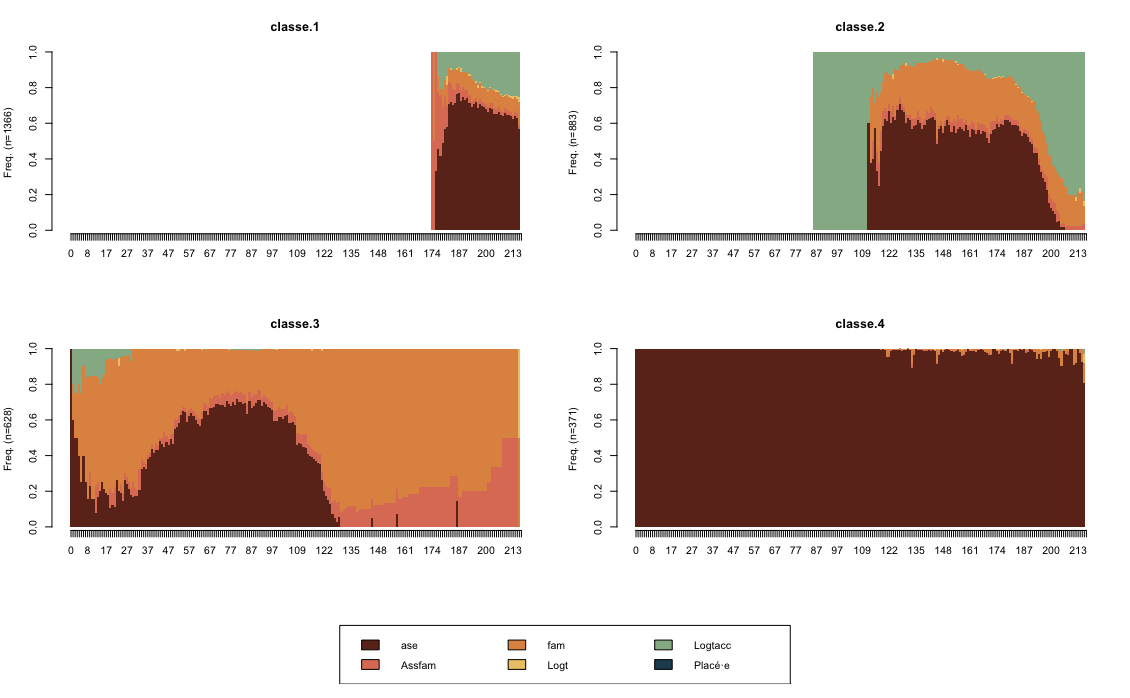
\includegraphics[width=0.8\linewidth]{Figure/Traj1} 

}

\caption{Chronogramme des différents parcours de placements à l'ASE}\label{fig:unnamed-chunk-38}
\end{figure}
\begin{flushright}
\small{Source : Enquête ES-PE 2017, DREES.
Champ : France entière, hors Mayotte, enfants sortis de l’établissement d’observation au cours de 2017 (hors sections d’accueil mères-enfants).}
\end{flushright}

Ainsi, quatre classes se détachent de la CAH qui est réalisée à l'aide
des résultats de l'Optimal Matching. La première concerne les
adolescents est est celle d'un placement temporaire avant la majorité,
caractérisée par un fort recours à l'internat collectif, et dans une
moindre mesure au logement autonome ou accompagné. La deuxième classe
semble s'apparenter à celle du placement autonome détecté dans notre
chapitre 4. Avec un recours au logement accompagné ou autonome au début
et à la fin de prise en charge. Avec une fois en MECS, une forte
importance de l'orientation en internat collectif. Les deux dernières
classes rassemblent des enfants connaissant un long parcours en
protection de l'enfance. La troisième classe est celle du maintien du
lien familial sous le contrôle des professionnels de la protection de
l'enfance avec le recours important au placement à domicile. La
quatrième classe est celle d'un long parcours en établissement de
placement et internat collectif.

\begin{quote}
\textbf{Optimal matching sur tous les enfants sortis en 2017}
\end{quote}

Voici maintenant les résultats de l'analyse des trajectoires réalisée
sur l'ensemble des enfants sortis en 2017 avant ou à leurs 18 ans. On
observe la forte part de l'étiquette ``placé·e'' correspondant à la
situation où nous savons que ces enfants sont placés, mais pas dans quel
type d'hébergement. On observe que la classe 3 obtenue par la CAH est
complètement occupée par les enfants sur lesquels nous n'avons pas
d'informations sur les types de placement précédents.

\begin{figure}[H]

{\centering \includegraphics[width=0.7\linewidth]{Global_files/figure-latex/unnamed-chunk-44-1} 

}

\caption{Chronogramme des différents parcours de placements à l'ASE}\label{fig:unnamed-chunk-44}
\end{figure}

\begin{figure}[H]

{\centering 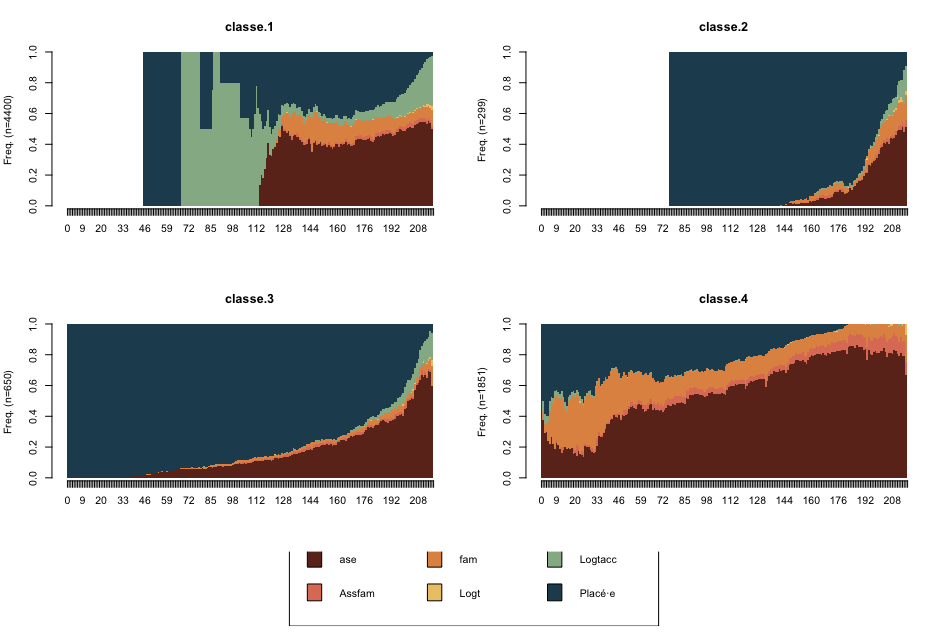
\includegraphics[width=0.8\linewidth]{Figure/Traj2} 

}

\caption{Chronogramme des différents parcours de placements à l'ASE}\label{fig:unnamed-chunk-48}
\end{figure}
\begin{flushright}
\small{Source : Enquête ES-PE 2017, DREES.
Champ : France entière, hors Mayotte, enfants sortis de l’établissement d’observation au cours de 2017 (hors sections d’accueil mères-enfants).}
\end{flushright}

\end{document}
